%&preformat-disser
\RequirePackage[l2tabu,orthodox]{nag} % Раскомментировав, можно в логе получать рекомендации относительно правильного использования пакетов и предупреждения об устаревших и нерекомендуемых пакетах
% Формат А4, 14pt (ГОСТ Р 7.0.11-2011, 5.3.6)
\documentclass[a4paper,14pt,oneside,openany]{memoir}

%%%%%%%%%%%%%%%%%%%%%%%%%%%%%%%%%%%%%%%%%%%%%%%%%%%%%%%%%%%%%%%%%%%%%%%%%%%%%%%%
%%%% Файл упрощённых настроек шаблона, общих для диссертации и автореферата %%%%
%%%%%%%%%%%%%%%%%%%%%%%%%%%%%%%%%%%%%%%%%%%%%%%%%%%%%%%%%%%%%%%%%%%%%%%%%%%%%%%%

%%% Режим черновика %%%
\makeatletter
\@ifundefined{c@draft}{
  \newcounter{draft}
  \setcounter{draft}{0}  % 0 --- чистовик (максимальное соблюдение ГОСТ)
                         % 1 --- черновик (отклонения от ГОСТ, но быстрая
                         %       сборка итоговых PDF)
}{}
\@ifundefined{myspec}{
  \newcounter{myspec}
  \setcounter{myspec}{1}  % 0 --- 05.13.18
                         % 1 --- 27.03.03
}{}
\makeatother

%%% Пометки в тексте %%%
\makeatletter
\@ifundefined{c@showmarkup}{
  \newcounter{showmarkup}
  \setcounter{showmarkup}{0}  % 0 --- скрыть пометки
                              % 1 --- показывать пометки
}{}
\makeatother

%%% Использование в pdflatex шрифтов не по-умолчанию %%%
\makeatletter
\@ifundefined{c@usealtfont}{
  \newcounter{usealtfont}
  \setcounter{usealtfont}{1}    % 0 --- шрифты на базе Computer Modern
                                % 1 --- использовать пакет pscyr, при его
                                %       наличии
                                % 2 --- использовать пакет XCharter, при наличии
                                %       подходящей версии
}{}
\makeatother

%%% Использование в xelatex и lualatex семейств шрифтов %%%
\makeatletter
\@ifundefined{c@fontfamily}{
  \newcounter{fontfamily}
  \setcounter{fontfamily}{1}  % 0 --- CMU семейство. Используется как fallback;
                              % 1 --- Шрифты от MS (Times New Roman и компания)
                              % 2 --- Семейство Liberation
}{}
\makeatother

%%% Библиография %%%
\makeatletter
\@ifundefined{c@bibliosel}{
  \newcounter{bibliosel}
  \setcounter{bibliosel}{1}   % 0 --- встроенная реализация с загрузкой файла
                              %       через движок bibtex8;
                              % 1 --- реализация пакетом biblatex через движок
                              %       biber
}{}
\makeatother

%%% Вывод типов ссылок в библиографии %%%
\makeatletter
\@ifundefined{c@mediadisplay}{
  \newcounter{mediadisplay}
  \setcounter{mediadisplay}{1}   % 0 --- не делать ничего; надписи [Текст] и
                                 %       [Эл. ресурс] будут выводиться только в ссылках с
                                 %       заполненным полем `media`;
                                 % 1 --- автоматически добавлять надпись [Текст] к ссылкам с
                                 %       незаполненным полем `media`; таким образом, у всех
                                 %       источников будет указан тип, что соответствует
                                 %       требованиям ГОСТ
                                 % 2 --- автоматически удалять надписи [Текст], [Эл. Ресурс] и др.;
                                 %       не соответствует ГОСТ
                                 % 3 --- автоматически удалять надпись [Текст];
                                 %       не соответствует ГОСТ
                                 % 4 --- автоматически удалять надпись [Эл. Ресурс];
                                 %       не соответствует ГОСТ
}{}
\makeatother

%%% Предкомпиляция tikz рисунков для ускорения работы %%%
\makeatletter
\@ifundefined{c@imgprecompile}{
  \newcounter{imgprecompile}
  \setcounter{imgprecompile}{0}   % 0 --- без предкомпиляции;
                                  % 1 --- пользоваться предварительно
                                  %       скомпилированными pdf вместо генерации
                                  %       заново из tikz
}{}
\makeatother
            % общие настройки шаблона

%%% Поля и разметка страницы %%%
\usepackage{pdflscape}  % Для включения альбомных страниц
\usepackage{geometry}   % Для последующего задания полей
\usepackage{listings}

%%% Проверка используемого TeX-движка %%%
\newif\ifxetexorluatex   % определяем новый условный оператор (http://tex.stackexchange.com/a/47579)
\ifxetex
    \xetexorluatextrue
\else
    \ifluatex
        \xetexorluatextrue
    \else
        \xetexorluatexfalse
    \fi
\fi

\newif\ifsynopsis           % Условие, проверяющее, что документ --- автореферат

\providebool{presentation}

\usepackage{comment}    % Позволяет убирать блоки текста (добавляет
                        % окружение comment и команду \excludecomment)

%%% Математические пакеты %%%
\usepackage{amsthm,amsmath,amscd}   % Математические дополнения от AMS
\usepackage{amsfonts,amssymb}       % Математические дополнения от AMS
\usepackage{mathtools}              % Добавляет окружение multlined
\usepackage{xfrac}                  % Красивые дроби
\usepackage[
    locale = DE,
    list-separator       = {;\,},
    list-final-separator = {;\,},
    list-pair-separator  = {;\,},
    list-units           = single,
    range-units          = single,
    range-phrase={\text{\ensuremath{-}}},
    % quotient-mode        = fraction, % красивые дроби могут не соответствовать ГОСТ
    fraction-function    = \sfrac,
    separate-uncertainty,
    ]{siunitx}[=v2]                 % Размерности SI
\sisetup{inter-unit-product = \ensuremath{{}\cdot{}}}

% Кириллица в нумерации subequations
% Для правильной работы требуется выполнение сразу после загрузки пакетов
\patchcmd{\subequations}{\def\theequation{\theparentequation\alph{equation}}}
{\def\theequation{\theparentequation\asbuk{equation}}}
{\typeout{subequations patched}}{\typeout{subequations not patched}}

%%%% Установки для размера шрифта 14 pt %%%%
%% Формирование переменных и констант для сравнения (один раз для всех подключаемых файлов)%%
%% должно располагаться до вызова пакета fontspec или polyglossia, потому что они сбивают его работу
\newlength{\curtextsize}
\newlength{\bigtextsize}
\setlength{\bigtextsize}{13.9pt}

\makeatletter
%\show\f@size    % неплохо для отслеживания, но вызывает стопорение процесса,
                 % если документ компилируется без команды  -interaction=nonstopmode
\setlength{\curtextsize}{\f@size pt}
\makeatother

%%% Кодировки и шрифты %%%
\ifxetexorluatex
    \ifpresentation
        \providecommand*\autodot{} % quick fix for polyglossia 1.50
    \fi
    \PassOptionsToPackage{no-math}{fontspec}    % https://tex.stackexchange.com/a/26295/104425
    \usepackage{polyglossia}[2014/05/21]        % Поддержка многоязычности
                                        % (fontspec подгружается автоматически)
\else
   %%% Решение проблемы копирования текста в буфер кракозябрами
    \ifnumequal{\value{usealtfont}}{0}{}{
        \input glyphtounicode.tex
        \input glyphtounicode-cmr.tex %from pdfx package
        \pdfgentounicode=1
    }
    \usepackage{cmap}   % Улучшенный поиск русских слов в полученном pdf-файле
    \ifnumequal{\value{usealtfont}}{2}{}{
        \defaulthyphenchar=127  % Если стоит до fontenc, то переносы
                                % не впишутся в выделяемый текст при
                                % копировании его в буфер обмена
    }
    \usepackage{textcomp}
    \usepackage[T1,T2A]{fontenc}                    % Поддержка русских букв
    \ifnumequal{\value{usealtfont}}{1}{% Используется pscyr, при наличии
        \IfFileExists{pscyr.sty}{\usepackage{pscyr}}{}  % Подключение pscyr
    }{}
    \usepackage[utf8]{inputenc}[2014/04/30]         % Кодировка utf8
    \usepackage[english, russian]{babel}[2014/03/24]% Языки: русский, английский
    \makeatletter\AtBeginDocument{\let\@elt\relax}\makeatother % babel 3.40 fix
    \ifnumequal{\value{usealtfont}}{2}{
        % http://dxdy.ru/post1238763.html#p1238763
        \usepackage[scaled=0.914]{XCharter}[2017/12/19] % Подключение русифицированных шрифтов XCharter
        \usepackage[charter, vvarbb, scaled=1.048]{newtxmath}[2017/12/14]
        \ifpresentation
        \else
            \setDisplayskipStretch{-0.078}
        \fi
    }{}
\fi

%%% Оформление абзацев %%%
\ifpresentation
\else
    \indentafterchapter     % Красная строка после заголовков типа chapter
    \usepackage{indentfirst}
\fi

%%% Цвета %%%
\ifpresentation
\else
    \usepackage[dvipsnames, table, hyperref]{xcolor} % Совместимо с tikz
\fi

%%% Таблицы %%%
\usepackage{longtable,ltcaption} % Длинные таблицы
\usepackage{multirow,makecell}   % Улучшенное форматирование таблиц
\usepackage{tabu, tabulary}      % таблицы с автоматически подбирающейся
                                 % шириной столбцов (tabu обязательно
                                 % до hyperref вызывать)
\makeatletter
%https://github.com/tabu-issues-for-future-maintainer/tabu/issues/26
\@ifpackagelater{longtable}{2020/02/07}{
\def\tabuendlongtrial{%
    \LT@echunk  \global\setbox\LT@gbox \hbox{\unhbox\LT@gbox}\kern\wd\LT@gbox
                \LT@get@widths
}%
}{}
\makeatother

\usepackage{threeparttable}      % автоматический подгон ширины подписи таблицы

%%% Общее форматирование
\usepackage{soulutf8}% Поддержка переносоустойчивых подчёркиваний и зачёркиваний
\usepackage{icomma}  % Запятая в десятичных дробях

%%% Оптимизация расстановки переносов и длины последней строки абзаца
\IfFileExists{impnattypo.sty}{% проверка установленности пакета impnattypo
    \ifluatex
        \ifnumequal{\value{draft}}{1}{% Черновик
            \usepackage[hyphenation, lastparline, nosingleletter, homeoarchy,
            rivers, draft]{impnattypo}
        }{% Чистовик
            \usepackage[hyphenation, lastparline, nosingleletter]{impnattypo}
        }
    \else
        \usepackage[hyphenation, lastparline]{impnattypo}
    \fi
}{}

%% Векторная графика

\usepackage{tikz}                   % Продвинутый пакет векторной графики
\usetikzlibrary{chains}             % Для примера tikz рисунка
\usetikzlibrary{shapes.geometric}   % Для примера tikz рисунка
\usetikzlibrary{shapes.symbols}     % Для примера tikz рисунка
\usetikzlibrary{arrows}             % Для примера tikz рисунка

%%% Гиперссылки %%%
\ifxetexorluatex
    \let\CYRDZE\relax
\fi
\usepackage{hyperref}[2012/11/06]

%%% Изображения %%%
\usepackage{graphicx}[2014/04/25]   % Подключаем пакет работы с графикой
\usepackage{caption}                % Подписи рисунков и таблиц
\usepackage{subcaption}             % Подписи подрисунков и подтаблиц
\usepackage{pdfpages}               % Добавление внешних pdf файлов

%%% Счётчики %%%
\usepackage{aliascnt}
\usepackage[figure,table]{totalcount}   % Счётчик рисунков и таблиц
\usepackage{totcount}   % Пакет создания счётчиков на основе последнего номера
                        % подсчитываемого элемента (может требовать дважды
                        % компилировать документ)
\usepackage{totpages}   % Счётчик страниц, совместимый с hyperref (ссылается
                        % на номер последней страницы). Желательно ставить
                        % последним пакетом в преамбуле

%%% Продвинутое управление групповыми ссылками (пока только формулами) %%%
\ifpresentation
\else
    \usepackage[russian]{cleveref} % cleveref имеет сложности со считыванием
    % языка из babel. Такое решение русификации вывода выбрано вместо
    % определения в documentclass из опасности что-то лишнее передать во все
    % остальные пакеты, включая библиографию.

    % Добавление возможности использования пробелов в \labelcref
    % https://tex.stackexchange.com/a/340502/104425
    \usepackage{kvsetkeys}
    \makeatletter
    \let\org@@cref\@cref
    \renewcommand*{\@cref}[2]{%
        \edef\process@me{%
            \noexpand\org@@cref{#1}{\zap@space#2 \@empty}%
        }\process@me
    }
    \makeatother
\fi

\usepackage{placeins} % для \FloatBarrier

\ifnumequal{\value{draft}}{1}{% Черновик
    \usepackage[firstpage]{draftwatermark}
    \SetWatermarkText{DRAFT}
    \SetWatermarkFontSize{14pt}
    \SetWatermarkScale{15}
    \SetWatermarkAngle{45}
}{}

%%% Цитата, не приводимая в автореферате:
% возможно, актуальна только для biblatex
%\newcommand{\citeinsynopsis}[1]{\ifsynopsis\else ~\cite{#1} \fi}

% если текущий процесс запущен библиотекой tikz-external, то прекомпиляция должна быть включена
\ifdefined\tikzexternalrealjob
    \setcounter{imgprecompile}{1}
\fi

\ifnumequal{\value{imgprecompile}}{1}{% Только если у нас включена предкомпиляция
    \usetikzlibrary{external}   % подключение возможности предкомпиляции
    \tikzexternalize[prefix=images/cache/,optimize command away=\includepdf] % activate! % здесь можно указать отдельную папку для скомпилированных файлов
    \ifxetex
        \tikzset{external/up to date check={diff}}
    \fi
}{}
         % Пакеты общие для диссертации и автореферата
\synopsisfalse                      % Этот документ --- не автореферат
%%% Прикладные пакеты %%%
%\usepackage{calc}               % Пакет для расчётов параметров, например длины

%%% Для добавления Стр. над номерами страниц в оглавлении
%%% http://tex.stackexchange.com/a/306950
\usepackage{afterpage}

%%% Списки %%%
\usepackage{enumitem}

%%% Оформление списка обозначений
\usepackage[intoc]{nomencl}
\makenomenclature
\setlength{\nomitemsep}{-.8\parsep}
    % Пакеты для диссертации
\usepackage{fr-longtable}    %ради \endlasthead

% Листинги с исходным кодом программ
\usepackage{fancyvrb}
\usepackage{listings}
\lccode`\~=0\relax %Без этого хака из-за особенностей пакета listings перестают работать конструкции с \MakeLowercase и т. п. в (xe|lua)latex

% Русская традиция начертания греческих букв
\usepackage{upgreek} % прямые греческие ради русской традиции

%%% Микротипографика
%\ifnumequal{\value{draft}}{0}{% Только если у нас режим чистовика
%    \usepackage[final, babel, shrink=45]{microtype}[2016/05/14] % улучшает представление букв и слов в строках, может помочь при наличии отдельно висящих слов
%}{}

% Отметка о версии черновика на каждой странице
% Чтобы работало надо в своей локальной копии по инструкции
% https://www.ctan.org/pkg/gitinfo2 создать небходимые файлы в папке
% ./git/hooks
% If you’re familiar with tweaking git, you can probably work it out for
% yourself. If not, I suggest you follow these steps:
% 1. First, you need a git repository and working tree. For this example,
% let’s suppose that the root of the working tree is in ~/compsci
% 2. Copy the file post-xxx-sample.txt (which is in the same folder of
% your TEX distribution as this pdf) into the git hooks directory in your
% working copy. In our example case, you should end up with a file called
% ~/compsci/.git/hooks/post-checkout
% 3. If you’re using a unix-like system, don’t forget to make the file executable.
% Just how you do this is outside the scope of this manual, but one
% possible way is with commands such as this:
% chmod g+x post-checkout.
% 4. Test your setup with “git checkout master” (or another suitable branch
% name). This should generate copies of gitHeadInfo.gin in the directories
% you intended.
% 5. Now make two more copies of this file in the same directory (hooks),
% calling them post-commit and post-merge, and you’re done. As before,
% users of unix-like systems should ensure these files are marked as
% executable.
\ifnumequal{\value{draft}}{1}{% Черновик
   \IfFileExists{.git/gitHeadInfo.gin}{
      \usepackage[mark,pcount]{gitinfo2}
      \renewcommand{\gitMark}{rev.\gitAbbrevHash\quad\gitCommitterEmail\quad\gitAuthorIsoDate}
      \renewcommand{\gitMarkFormat}{\rmfamily\color{Gray}\small\bfseries}
   }{}
}{}   % Пакеты для специфических пользовательских задач

%%%%%%%%%%%%%%%%%%%%%%%%%%%%%%%%%%%%%%%%%%%%%%%%%%%%%%
%%%% Файл упрощённых настроек шаблона диссертации %%%%
%%%%%%%%%%%%%%%%%%%%%%%%%%%%%%%%%%%%%%%%%%%%%%%%%%%%%%

%%% Инициализирование переменных, не трогать!  %%%
\newcounter{intvl}
\newcounter{otstup}
\newcounter{contnumeq}
\newcounter{contnumfig}
\newcounter{contnumtab}
\newcounter{pgnum}
\newcounter{chapstyle}
\newcounter{headingdelim}
\newcounter{headingalign}
\newcounter{headingsize}
%%%%%%%%%%%%%%%%%%%%%%%%%%%%%%%%%%%%%%%%%%%%%%%%%%%%%%

\newcommand{\mycite}[2]{~\autocite{#1}}
\newcommand{\ifdisser}[2]{#1}

%%% Область упрощённого управления оформлением %%%

%% Интервал между заголовками и между заголовком и текстом %%
% Заголовки отделяют от текста сверху и снизу
% тремя интервалами (ГОСТ Р 7.0.11-2011, 5.3.5)
\setcounter{intvl}{3}               % Коэффициент кратности к размеру шрифта

%% Отступы у заголовков в тексте %%
\setcounter{otstup}{0}              % 0 --- без отступа; 1 --- абзацный отступ

%% Нумерация формул, таблиц и рисунков %%
% Нумерация формул
\setcounter{contnumeq}{0}   % 0 --- пораздельно (во введении подряд,
                            %       без номера раздела);
                            % 1 --- сквозная нумерация по всей диссертации
% Нумерация рисунков
\setcounter{contnumfig}{0}  % 0 --- пораздельно (во введении подряд,
                            %       без номера раздела);
                            % 1 --- сквозная нумерация по всей диссертации
% Нумерация таблиц
\setcounter{contnumtab}{1}  % 0 --- пораздельно (во введении подряд,
                            %       без номера раздела);
                            % 1 --- сквозная нумерация по всей диссертации

%% Оглавление %%
\setcounter{pgnum}{1}       % 0 --- номера страниц никак не обозначены;
                            % 1 --- Стр. над номерами страниц (дважды
                            %       компилировать после изменения настройки)
\settocdepth{subsection}    % до какого уровня подразделов выносить в оглавление
\setsecnumdepth{subsection} % до какого уровня нумеровать подразделы


%% Текст и форматирование заголовков %%
\setcounter{chapstyle}{1}     % 0 --- разделы только под номером;
                              % 1 --- разделы с названием "Глава" перед номером
\setcounter{headingdelim}{1}  % 0 --- номер отделен пропуском в 1em или \quad;
                              % 1 --- номера разделов и приложений отделены
                              %       точкой с пробелом, подразделы пропуском
                              %       без точки;
                              % 2 --- номера разделов, подразделов и приложений
                              %       отделены точкой с пробелом.

%% Выравнивание заголовков в тексте %%
\setcounter{headingalign}{0}  % 0 --- по центру;
                              % 1 --- по левому краю

%% Размеры заголовков в тексте %%
\setcounter{headingsize}{0}   % 0 --- по ГОСТ, все всегда 14 пт;
                              % 1 --- пропорционально изменяющийся размер
                              %       в зависимости от базового шрифта

%% Подпись таблиц %%

% Смещение строк подписи после первой строки
\newcommand{\tabindent}{0cm}

% Тип форматирования заголовка таблицы:
% plain --- название и текст в одной строке
% split --- название и текст в разных строках
\newcommand{\tabformat}{plain}

%%% Настройки форматирования таблицы `plain`

% Выравнивание по центру подписи, состоящей из одной строки:
% true  --- выравнивать
% false --- не выравнивать
\newcommand{\tabsinglecenter}{false}

% Выравнивание подписи таблиц:
% justified   --- выравнивать как обычный текст («по ширине»)
% centering   --- выравнивать по центру
% centerlast  --- выравнивать по центру только последнюю строку
% centerfirst --- выравнивать по центру только первую строку (не рекомендуется)
% raggedleft  --- выравнивать по правому краю
% raggedright --- выравнивать по левому краю
\newcommand{\tabjust}{justified}

% Разделитель записи «Таблица #» и названия таблицы
\newcommand{\tablabelsep}{~\cyrdash\ }

%%% Настройки форматирования таблицы `split`

% Положение названия таблицы:
% \centering   --- выравнивать по центру
% \raggedleft  --- выравнивать по правому краю
% \raggedright --- выравнивать по левому краю
\newcommand{\splitformatlabel}{\raggedleft}

% Положение текста подписи:
% \centering   --- выравнивать по центру
% \raggedleft  --- выравнивать по правому краю
% \raggedright --- выравнивать по левому краю
\newcommand{\splitformattext}{\raggedright}

%% Подпись рисунков %%
%Разделитель записи «Рисунок #» и названия рисунка
\newcommand{\figlabelsep}{~\cyrdash\ }  % (ГОСТ 2.105, 4.3.1)
                                        % "--- здесь не работает

%%% Цвета гиперссылок %%%
% Latex color definitions: http://latexcolor.com/
\definecolor{linkcolor}{rgb}{0.9,0,0}
\definecolor{citecolor}{rgb}{0,0.6,0}
\definecolor{urlcolor}{rgb}{0,0,1}
%\definecolor{linkcolor}{rgb}{0,0,0} %black
%\definecolor{citecolor}{rgb}{0,0,0} %black
%\definecolor{urlcolor}{rgb}{0,0,0} %black
      % Упрощённые настройки шаблона

% Новые переменные, которые могут использоваться во всём проекте
% ГОСТ 7.0.11-2011
% 9.2 Оформление текста автореферата диссертации
% 9.2.1 Общая характеристика работы включает в себя следующие основные структурные
% элементы:
% актуальность темы исследования;
\newcommand{\actualityTXT}{Актуальность темы.}
% степень ее разработанности;
\newcommand{\progressTXT}{Степень разработанности темы.}
% цели и задачи;
\newcommand{\aimTXT}{Целью}
\newcommand{\tasksTXT}{задачи}
% научную новизну;
\newcommand{\noveltyTXT}{Научная новизна:}
% теоретическую и практическую значимость работы;
%\newcommand{\influenceTXT}{Теоретическая и практическая значимость}
% или чаще используют просто
\newcommand{\influenceTXT}{Практическая значимость}
% методологию и методы исследования;
\newcommand{\methodsTXT}{Методология и методы исследования.}
% положения, выносимые на защиту;
\newcommand{\defpositionsTXT}{Основные положения, выносимые на~защиту:}
% степень достоверности и апробацию результатов.
\newcommand{\reliabilityTXT}{Достоверность}
\newcommand{\probationTXT}{Апробация работы.}

\newcommand{\contributionTXT}{Личный вклад.}
\newcommand{\publicationsTXT}{Публикации.}


%%% Заголовки библиографии:

% для автореферата:
\newcommand{\bibtitleauthor}{Публикации автора по теме диссертации}

% для стиля библиографии `\insertbiblioauthorgrouped`
\newcommand{\bibtitleauthorvak}{В изданиях из списка ВАК РФ}
\newcommand{\bibtitleauthorscopus}{В изданиях, входящих в международную базу цитирования Scopus}
\newcommand{\bibtitleauthorwos}{В изданиях, входящих в международную базу цитирования Web of Science}
\newcommand{\bibtitleauthorother}{В прочих изданиях}
\newcommand{\bibtitleauthorconf}{В сборниках трудов конференций}
\newcommand{\bibtitleauthorpatent}{Зарегистрированные патенты}
\newcommand{\bibtitleauthorprogram}{Зарегистрированные программы для ЭВМ}

% для стиля библиографии `\insertbiblioauthorimportant`:
\newcommand{\bibtitleauthorimportant}{Наиболее значимые \protect\MakeLowercase\bibtitleauthor}

% для списка литературы в диссертации и списка чужих работ в автореферате:
\newcommand{\bibtitlefull}{Список литературы} % (ГОСТ Р 7.0.11-2011, 4)
         % Новые переменные, для всего проекта

%%% Основные сведения %%%
\newcommand{\thesisAuthorLastName}{Тюнин}
\newcommand{\thesisAuthorOtherNames}{Николай Николаевич}
\newcommand{\thesisAuthorInitials}{Н.\,Н.}
\newcommand{\thesisAuthor}             % Диссертация, ФИО автора
{%
    \texorpdfstring{% \texorpdfstring takes two arguments and uses the first for (La)TeX and the second for pdf
        \thesisAuthorLastName~\thesisAuthorOtherNames% так будет отображаться на титульном листе или в тексте, где будет использоваться переменная
    }{%
        \thesisAuthorLastName, \thesisAuthorOtherNames% эта запись для свойств pdf-файла. В таком виде, если pdf будет обработан программами для сбора библиографических сведений, будет правильно представлена фамилия.
    }
}
\newcommand{\thesisAuthorShort}        % Диссертация, ФИО автора инициалами
{\thesisAuthorInitials~\thesisAuthorLastName}
%\newcommand{\thesisUdk}                % Диссертация, УДК
%{\fixme{xxx.xxx}}
\newcommand{\thesisTitle}              % Диссертация, название
{Анализ и решение задач оптимизации направленности фазированных антенных решеток коротковолнового диапазона}

\ifnumequal{\value{myspec}}{0}{
    \newcommand{\thesisSpecialtyNumber}    % Диссертация, специальность, номер
    {05.13.18}
    \newcommand{\thesisSpecialtyTitle}     % Диссертация, специальность, название (название взято с сайта ВАК для примера)
    {Математическое моделирование, численные методы и~комплексы программ}
}{
    \newcommand{\thesisSpecialtyNumber}    % Диссертация, специальность, номер
    {2.3.1}
    \newcommand{\thesisSpecialtyTitle}     % Диссертация, специальность, название (название взято с сайта ВАК для примера)
    {Системный анализ, управление и обработка информации}
}

%% \newcommand{\thesisSpecialtyTwoNumber} % Диссертация, вторая специальность, номер
%% {\fixme{XX.XX.XX}}
%% \newcommand{\thesisSpecialtyTwoTitle}  % Диссертация, вторая специальность, название
%% {\fixme{Теория и~методика физического воспитания, спортивной тренировки,
%% оздоровительной и~адаптивной физической культуры}}
\newcommand{\thesisDegree}             % Диссертация, ученая степень
{кандидата технических наук}
\newcommand{\thesisDegreeShort}        % Диссертация, ученая степень, краткая запись
{канд. тех. наук}
\newcommand{\thesisCity}               % Диссертация, город написания диссертации
{Омск}
\newcommand{\thesisYear}               % Диссертация, год написания диссертации
{\the\year}
\newcommand{\thesisOrganization}       % Диссертация, организация
{Омский филиал Федерального государственного бюджетного учреждения науки Института математики им. С.Л. Соболева Сибирского отделения Российской академии наук (ОФ ИМ СО РАН)}
\newcommand{\thesisOrganizationShort}  % Диссертация, краткое название организации для доклада
{Оптимизация направленности}

\newcommand{\thesisInOrganization}     % Диссертация, организация в предложном падеже: Работа выполнена в ...
{Омском филиале Федерального государственного бюджетного учреждения науки Института математики им. С.Л. Соболева Сибирского отделения Российской академии наук (ОФ ИМ СО РАН)}

%% \newcommand{\supervisorDead}{}           % Рисовать рамку вокруг фамилии
\newcommand{\supervisorFio}              % Научный руководитель, ФИО
{Еремеев Антон Валентинович}
\newcommand{\supervisorRegalia}          % Научный руководитель, регалии
{доктор~физико-математических~наук,~доцент}
\newcommand{\supervisorFioShort}         % Научный руководитель, ФИО
{А.\,В.~Евемеев}
\newcommand{\supervisorRegaliaShort}     % Научный руководитель, регалии
{д.ф.-м.н.,~доц.}

%% \newcommand{\supervisorTwoDead}{}        % Рисовать рамку вокруг фамилии
%% \newcommand{\supervisorTwoFio}           % Второй научный руководитель, ФИО
%% {\fixme{Фамилия Имя Отчество}}
%% \newcommand{\supervisorTwoRegalia}       % Второй научный руководитель, регалии
%% {\fixme{уч. степень, уч. звание}}
%% \newcommand{\supervisorTwoFioShort}      % Второй научный руководитель, ФИО
%% {\fixme{И.\,О.~Фамилия}}
%% \newcommand{\supervisorTwoRegaliaShort}  % Второй научный руководитель, регалии
%% {\fixme{уч.~ст.,~уч.~зв.}}

\newcommand{\opponentOneFio}           % Оппонент 1, ФИО
{Картак Вадим Михайлович}
\newcommand{\opponentOneRegalia}       % Оппонент 1, регалии
{доктор физико-математических наук, профессор}
\newcommand{\opponentOneJobPlace}      % Оппонент 1, место работы
{Уфимский государственный авиационный технический университет}
\newcommand{\opponentOneJobPost}       % Оппонент 1, должность
{заведующий кафедрой}

\newcommand{\opponentTwoFio}           % Оппонент 2, ФИО
{Груздева Татьяна Владимировна}
\newcommand{\opponentTwoRegalia}       % Оппонент 2, регалии
{кандидат физико-математических наук}
\newcommand{\opponentTwoJobPlace}      % Оппонент 2, место работы
{Институт динамики систем и теории управления имени В.М. Матросова Сибирского отделения Российской академии наук}
\newcommand{\opponentTwoJobPost}       % Оппонент 2, должность
{старший научный сотрудник}

%% \newcommand{\opponentThreeFio}         % Оппонент 3, ФИО
%% {\fixme{Фамилия Имя Отчество}}
%% \newcommand{\opponentThreeRegalia}     % Оппонент 3, регалии
%% {\fixme{кандидат физико-математических наук}}
%% \newcommand{\opponentThreeJobPlace}    % Оппонент 3, место работы
%% {\fixme{Основное место работы c длинным длинным длинным длинным названием}}
%% \newcommand{\opponentThreeJobPost}     % Оппонент 3, должность
%% {\fixme{старший научный сотрудник}}

\newcommand{\leadingOrganizationTitle} % Ведущая организация, дополнительные строки. Удалить, чтобы не отображать в автореферате
{Федеральное государственное автономное образовательное учреждение высшего образования <<Омский государственный технический университет>>}

\newcommand{\defenseDate}              % Защита, дата
{"\underline{\phantom{0111}}"~~"\underline{\phantom{сентябрясент}}~\the\year~г.~в~\underline{\phantom{0111}}~часов}
\newcommand{\defenseCouncilNumber}     % Защита, номер диссертационного совета
{Д\,24.2.403.01}
\newcommand{\defenseCouncilTitle}      % Защита, учреждение диссертационного совета
{Сибирский государственный университет науки и технологий имени академика М.Ф. Решетнева}
\newcommand{\defenseCouncilAddress}    % Защита, адрес учреждение диссертационного совета
{660037 г. Красноярск, проспект имени газеты «Красноярский рабочий», 31}
\newcommand{\defenseCouncilPhone}      % Телефон для справок
{\fixme{+7~(0000)~00-00-00}}

\newcommand{\defenseSecretaryFio}      % Секретарь диссертационного совета, ФИО
{Панфилов Илья Александрович}
\newcommand{\defenseSecretaryRegalia}  % Секретарь диссертационного совета, регалии
{кандидат технических наук, доцент}            % Для сокращений есть ГОСТы, например: ГОСТ Р 7.0.12-2011 + http://base.garant.ru/179724/#block_30000

\newcommand{\synopsisLibrary}          % Автореферат, название библиотеки
{ФГБОУ ВО <<Сибирский государственный университет науки и технологий имени академика М.Ф. Решетнева>> и на сайте https://www.sibsau.ru}
\newcommand{\synopsisDate}             % Автореферат, дата рассылки
{"\underline{\phantom{0111}}"~~"\underline{\phantom{сентябрясент}}"~\the\year~года}

% To avoid conflict with beamer class use \providecommand
\providecommand{\keywords}%            % Ключевые слова для метаданных PDF диссертации и автореферата
{}
             % Основные сведения
%%% Кодировки и шрифты %%%
\ifxetexorluatex
    % Язык по-умолчанию русский с поддержкой приятных команд пакета babel
    \setmainlanguage[babelshorthands=true]{russian}
    % Дополнительный язык = английский (в американской вариации по-умолчанию)
    \setotherlanguage{english}

    % Проверка существования шрифтов. Недоступна в pdflatex
    \ifnumequal{\value{fontfamily}}{1}{
        \IfFontExistsTF{Times New Roman}{}{\setcounter{fontfamily}{0}}
    }{}
    \ifnumequal{\value{fontfamily}}{2}{
        \IfFontExistsTF{LiberationSerif}{}{\setcounter{fontfamily}{0}}
    }{}

    \ifnumequal{\value{fontfamily}}{0}{                    % Семейство шрифтов CMU. Используется как fallback
        \setmonofont{CMU Typewriter Text}                  % моноширинный шрифт
        \newfontfamily\cyrillicfonttt{CMU Typewriter Text} % моноширинный шрифт для кириллицы
        \defaultfontfeatures{Ligatures=TeX}                % стандартные лигатуры TeX, замены нескольких дефисов на тире и т. п. Настройки моноширинного шрифта должны идти до этой строки, чтобы при врезках кода программ в коде не применялись лигатуры и замены дефисов
        \setmainfont{CMU Serif}                            % Шрифт с засечками
        \newfontfamily\cyrillicfont{CMU Serif}             % Шрифт с засечками для кириллицы
        \setsansfont{CMU Sans Serif}                       % Шрифт без засечек
        \newfontfamily\cyrillicfontsf{CMU Sans Serif}      % Шрифт без засечек для кириллицы
    }

    \ifnumequal{\value{fontfamily}}{1}{                    % Семейство MS шрифтов
        \setmonofont{Courier New}                          % моноширинный шрифт
        \newfontfamily\cyrillicfonttt{Courier New}         % моноширинный шрифт для кириллицы
        \defaultfontfeatures{Ligatures=TeX}                % стандартные лигатуры TeX, замены нескольких дефисов на тире и т. п. Настройки моноширинного шрифта должны идти до этой строки, чтобы при врезках кода программ в коде не применялись лигатуры и замены дефисов
        \setmainfont{Times New Roman}                      % Шрифт с засечками
        \newfontfamily\cyrillicfont{Times New Roman}       % Шрифт с засечками для кириллицы
        \setsansfont{Arial}                                % Шрифт без засечек
        \newfontfamily\cyrillicfontsf{Arial}               % Шрифт без засечек для кириллицы
    }

    \ifnumequal{\value{fontfamily}}{2}{                    % Семейство шрифтов Liberation (https://pagure.io/liberation-fonts)
        \setmonofont{LiberationMono}[Scale=0.87] % моноширинный шрифт
        \newfontfamily\cyrillicfonttt{LiberationMono}[     % моноширинный шрифт для кириллицы
            Scale=0.87]
        \defaultfontfeatures{Ligatures=TeX}                % стандартные лигатуры TeX, замены нескольких дефисов на тире и т. п. Настройки моноширинного шрифта должны идти до этой строки, чтобы при врезках кода программ в коде не применялись лигатуры и замены дефисов
        \setmainfont{LiberationSerif}                      % Шрифт с засечками
        \newfontfamily\cyrillicfont{LiberationSerif}       % Шрифт с засечками для кириллицы
        \setsansfont{LiberationSans}                       % Шрифт без засечек
        \newfontfamily\cyrillicfontsf{LiberationSans}      % Шрифт без засечек для кириллицы
    }

\else
    \ifnumequal{\value{usealtfont}}{1}{% Используется pscyr, при наличии
        \IfFileExists{pscyr.sty}{\renewcommand{\rmdefault}{ftm}}{}
    }{}
\fi
            % Определение шрифтов (частичное)
%%% Шаблон %%%
\DeclareRobustCommand{\fixme}{\textcolor{red}}  % решаем проблему превращения
                                % названия цвета в результате \MakeUppercase,
                                % http://tex.stackexchange.com/a/187930,
                                % \DeclareRobustCommand protects \fixme
                                % from expanding inside \MakeUppercase
\AtBeginDocument{%
    \setlength{\parindent}{2.5em}                   % Абзацный отступ. Должен быть одинаковым по всему тексту и равен пяти знакам (ГОСТ Р 7.0.11-2011, 5.3.7).
}

%%% Таблицы %%%
\DeclareCaptionLabelSeparator{tabsep}{\tablabelsep} % нумерация таблиц
\DeclareCaptionFormat{split}{\splitformatlabel#1\par\splitformattext#3}

\captionsetup[table]{
        format=\tabformat,                % формат подписи (plain|hang)
        font=normal,                      % нормальные размер, цвет, стиль шрифта
        skip=.0pt,                        % отбивка под подписью
        parskip=.0pt,                     % отбивка между параграфами подписи
        position=above,                   % положение подписи
        justification=\tabjust,           % центровка
        indent=\tabindent,                % смещение строк после первой
        labelsep=tabsep,                  % разделитель
        singlelinecheck=\tabsinglecenter, % не выравнивать по центру, если умещается в одну строку
}

%%% Рисунки %%%
\DeclareCaptionLabelSeparator{figsep}{\figlabelsep} % нумерация рисунков

\captionsetup[figure]{
        format=plain,                     % формат подписи (plain|hang)
        font=normal,                      % нормальные размер, цвет, стиль шрифта
        skip=.0pt,                        % отбивка под подписью
        parskip=.0pt,                     % отбивка между параграфами подписи
        position=below,                   % положение подписи
        singlelinecheck=true,             % выравнивание по центру, если умещается в одну строку
        justification=centerlast,         % центровка
        labelsep=figsep,                  % разделитель
}

%%% Подписи подрисунков %%%
\DeclareCaptionSubType{figure}
\renewcommand\thesubfigure{\asbuk{subfigure}} % нумерация подрисунков
\ifsynopsis
\DeclareCaptionFont{norm}{\fontsize{10pt}{11pt}\selectfont}
\newcommand{\subfigureskip}{2.pt}
\else
\DeclareCaptionFont{norm}{\fontsize{14pt}{16pt}\selectfont}
\newcommand{\subfigureskip}{0.pt}
\fi

\captionsetup[subfloat]{
        labelfont=norm,                 % нормальный размер подписей подрисунков
        textfont=norm,                  % нормальный размер подписей подрисунков
        labelsep=space,                 % разделитель
        labelformat=brace,              % одна скобка справа от номера
        justification=centering,        % центровка
        singlelinecheck=true,           % выравнивание по центру, если умещается в одну строку
        skip=\subfigureskip,            % отбивка над подписью
        parskip=.0pt,                   % отбивка между параграфами подписи
        position=below,                 % положение подписи
}

%%% Настройки ссылок на рисунки, таблицы и др. %%%
% команды \cref...format отвечают за форматирование при помощи команды \cref
% команды \labelcref...format отвечают за форматирование при помощи команды \labelcref

\ifpresentation
\else
    \crefdefaultlabelformat{#2#1#3}

    % Уравнение
    \crefformat{equation}{(#2#1#3)} % одиночная ссылка с приставкой
    \labelcrefformat{equation}{(#2#1#3)} % одиночная ссылка без приставки
    \crefrangeformat{equation}{(#3#1#4) \cyrdash~(#5#2#6)} % диапазон ссылок с приставкой
    \labelcrefrangeformat{equation}{(#3#1#4) \cyrdash~(#5#2#6)} % диапазон ссылок без приставки
    \crefmultiformat{equation}{(#2#1#3)}{ и~(#2#1#3)}{, (#2#1#3)}{ и~(#2#1#3)} % перечисление ссылок с приставкой
    \labelcrefmultiformat{equation}{(#2#1#3)}{ и~(#2#1#3)}{, (#2#1#3)}{ и~(#2#1#3)} % перечисление без приставки

    % Подуравнение
    \crefformat{subequation}{(#2#1#3)} % одиночная ссылка с приставкой
    \labelcrefformat{subequation}{(#2#1#3)} % одиночная ссылка без приставки
    \crefrangeformat{subequation}{(#3#1#4) \cyrdash~(#5#2#6)} % диапазон ссылок с приставкой
    \labelcrefrangeformat{subequation}{(#3#1#4) \cyrdash~(#5#2#6)} % диапазон ссылок без приставки
    \crefmultiformat{subequation}{(#2#1#3)}{ и~(#2#1#3)}{, (#2#1#3)}{ и~(#2#1#3)} % перечисление ссылок с приставкой
    \labelcrefmultiformat{subequation}{(#2#1#3)}{ и~(#2#1#3)}{, (#2#1#3)}{ и~(#2#1#3)} % перечисление без приставки

    % Глава
    \crefformat{chapter}{#2#1#3} % одиночная ссылка с приставкой
    \labelcrefformat{chapter}{#2#1#3} % одиночная ссылка без приставки
    \crefrangeformat{chapter}{#3#1#4 \cyrdash~#5#2#6} % диапазон ссылок с приставкой
    \labelcrefrangeformat{chapter}{#3#1#4 \cyrdash~#5#2#6} % диапазон ссылок без приставки
    \crefmultiformat{chapter}{#2#1#3}{ и~#2#1#3}{, #2#1#3}{ и~#2#1#3} % перечисление ссылок с приставкой
    \labelcrefmultiformat{chapter}{#2#1#3}{ и~#2#1#3}{, #2#1#3}{ и~#2#1#3} % перечисление без приставки

    % Параграф
    \crefformat{section}{#2#1#3} % одиночная ссылка с приставкой
    \labelcrefformat{section}{#2#1#3} % одиночная ссылка без приставки
    \crefrangeformat{section}{#3#1#4 \cyrdash~#5#2#6} % диапазон ссылок с приставкой
    \labelcrefrangeformat{section}{#3#1#4 \cyrdash~#5#2#6} % диапазон ссылок без приставки
    \crefmultiformat{section}{#2#1#3}{ и~#2#1#3}{, #2#1#3}{ и~#2#1#3} % перечисление ссылок с приставкой
    \labelcrefmultiformat{section}{#2#1#3}{ и~#2#1#3}{, #2#1#3}{ и~#2#1#3} % перечисление без приставки

    % Приложение
    \crefformat{appendix}{#2#1#3} % одиночная ссылка с приставкой
    \labelcrefformat{appendix}{#2#1#3} % одиночная ссылка без приставки
    \crefrangeformat{appendix}{#3#1#4 \cyrdash~#5#2#6} % диапазон ссылок с приставкой
    \labelcrefrangeformat{appendix}{#3#1#4 \cyrdash~#5#2#6} % диапазон ссылок без приставки
    \crefmultiformat{appendix}{#2#1#3}{ и~#2#1#3}{, #2#1#3}{ и~#2#1#3} % перечисление ссылок с приставкой
    \labelcrefmultiformat{appendix}{#2#1#3}{ и~#2#1#3}{, #2#1#3}{ и~#2#1#3} % перечисление без приставки

    % Рисунок
    \crefformat{figure}{#2#1#3} % одиночная ссылка с приставкой
    \labelcrefformat{figure}{#2#1#3} % одиночная ссылка без приставки
    \crefrangeformat{figure}{#3#1#4 \cyrdash~#5#2#6} % диапазон ссылок с приставкой
    \labelcrefrangeformat{figure}{#3#1#4 \cyrdash~#5#2#6} % диапазон ссылок без приставки
    \crefmultiformat{figure}{#2#1#3}{ и~#2#1#3}{, #2#1#3}{ и~#2#1#3} % перечисление ссылок с приставкой
    \labelcrefmultiformat{figure}{#2#1#3}{ и~#2#1#3}{, #2#1#3}{ и~#2#1#3} % перечисление без приставки

    % Таблица
    \crefformat{table}{#2#1#3} % одиночная ссылка с приставкой
    \labelcrefformat{table}{#2#1#3} % одиночная ссылка без приставки
    \crefrangeformat{table}{#3#1#4 \cyrdash~#5#2#6} % диапазон ссылок с приставкой
    \labelcrefrangeformat{table}{#3#1#4 \cyrdash~#5#2#6} % диапазон ссылок без приставки
    \crefmultiformat{table}{#2#1#3}{ и~#2#1#3}{, #2#1#3}{ и~#2#1#3} % перечисление ссылок с приставкой
    \labelcrefmultiformat{table}{#2#1#3}{ и~#2#1#3}{, #2#1#3}{ и~#2#1#3} % перечисление без приставки

    % Листинг
    \crefformat{lstlisting}{#2#1#3} % одиночная ссылка с приставкой
    \labelcrefformat{lstlisting}{#2#1#3} % одиночная ссылка без приставки
    \crefrangeformat{lstlisting}{#3#1#4 \cyrdash~#5#2#6} % диапазон ссылок с приставкой
    \labelcrefrangeformat{lstlisting}{#3#1#4 \cyrdash~#5#2#6} % диапазон ссылок без приставки
    \crefmultiformat{lstlisting}{#2#1#3}{ и~#2#1#3}{, #2#1#3}{ и~#2#1#3} % перечисление ссылок с приставкой
    \labelcrefmultiformat{lstlisting}{#2#1#3}{ и~#2#1#3}{, #2#1#3}{ и~#2#1#3} % перечисление без приставки

    % Листинг
    \crefformat{ListingEnv}{#2#1#3} % одиночная ссылка с приставкой
    \labelcrefformat{ListingEnv}{#2#1#3} % одиночная ссылка без приставки
    \crefrangeformat{ListingEnv}{#3#1#4 \cyrdash~#5#2#6} % диапазон ссылок с приставкой
    \labelcrefrangeformat{ListingEnv}{#3#1#4 \cyrdash~#5#2#6} % диапазон ссылок без приставки
    \crefmultiformat{ListingEnv}{#2#1#3}{ и~#2#1#3}{, #2#1#3}{ и~#2#1#3} % перечисление ссылок с приставкой
    \labelcrefmultiformat{ListingEnv}{#2#1#3}{ и~#2#1#3}{, #2#1#3}{ и~#2#1#3} % перечисление без приставки
\fi

%%% Настройки гиперссылок %%%
\ifluatex
    \hypersetup{
        unicode,                % Unicode encoded PDF strings
    }
\fi

\hypersetup{
    linktocpage=true,           % ссылки с номера страницы в оглавлении, списке таблиц и списке рисунков
%    linktoc=all,                % both the section and page part are links
%    pdfpagelabels=false,        % set PDF page labels (true|false)
    plainpages=false,           % Forces page anchors to be named by the Arabic form  of the page number, rather than the formatted form
    colorlinks,                 % ссылки отображаются раскрашенным текстом, а не раскрашенным прямоугольником, вокруг текста
    linkcolor={linkcolor},      % цвет ссылок типа ref, eqref и подобных
    citecolor={citecolor},      % цвет ссылок-цитат
    urlcolor={urlcolor},        % цвет гиперссылок
%    hidelinks,                  % Hide links (removing color and border)
    pdftitle={\thesisTitle},    % Заголовок
    pdfauthor={\thesisAuthor},  % Автор
    pdfsubject={\thesisSpecialtyNumber\ \thesisSpecialtyTitle},      % Тема
%    pdfcreator={Создатель},     % Создатель, Приложение
%    pdfproducer={Производитель},% Производитель, Производитель PDF
    pdfkeywords={\keywords},    % Ключевые слова
    pdflang={ru},
}
\ifnumequal{\value{draft}}{1}{% Черновик
    \hypersetup{
        draft,
    }
}{}

%%% Списки %%%
% Используем короткое тире (endash) для ненумерованных списков (ГОСТ 2.105-95, пункт 4.1.7, требует дефиса, но так лучше смотрится)
\renewcommand{\labelitemi}{\normalfont\bfseries{--}}

% Перечисление строчными буквами латинского алфавита (ГОСТ 2.105-95, 4.1.7)
%\renewcommand{\theenumi}{\alph{enumi}}
%\renewcommand{\labelenumi}{\theenumi)}

% Перечисление строчными буквами русского алфавита (ГОСТ 2.105-95, 4.1.7)
\makeatletter
\AddEnumerateCounter{\asbuk}{\russian@alph}{щ}      % Управляем списками/перечислениями через пакет enumitem, а он 'не знает' про asbuk, потому 'учим' его
\makeatother
%\renewcommand{\theenumi}{\asbuk{enumi}} %первый уровень нумерации
%\renewcommand{\labelenumi}{\theenumi)} %первый уровень нумерации
\renewcommand{\theenumii}{\asbuk{enumii}} %второй уровень нумерации
\renewcommand{\labelenumii}{\theenumii)} %второй уровень нумерации
\renewcommand{\theenumiii}{\arabic{enumiii}} %третий уровень нумерации
\renewcommand{\labelenumiii}{\theenumiii)} %третий уровень нумерации

\setlist{nosep,%                                    % Единый стиль для всех списков (пакет enumitem), без дополнительных интервалов.
    labelindent=\parindent,leftmargin=*%            % Каждый пункт, подпункт и перечисление записывают с абзацного отступа (ГОСТ 2.105-95, 4.1.8)
}

%%% Правильная нумерация приложений, рисунков и формул %%%
%% По ГОСТ 2.105, п. 4.3.8 Приложения обозначают заглавными буквами русского алфавита,
%% начиная с А, за исключением букв Ё, З, Й, О, Ч, Ь, Ы, Ъ.
%% Здесь также переделаны все нумерации русскими буквами.
\ifxetexorluatex
    \makeatletter
    \def\russian@Alph#1{\ifcase#1\or
       А\or Б\or В\or Г\or Д\or Е\or Ж\or
       И\or К\or Л\or М\or Н\or
       П\or Р\or С\or Т\or У\or Ф\or Х\or
       Ц\or Ш\or Щ\or Э\or Ю\or Я\else\xpg@ill@value{#1}{russian@Alph}\fi}
    \def\russian@alph#1{\ifcase#1\or
       а\or б\or в\or г\or д\or е\or ж\or
       и\or к\or л\or м\or н\or
       п\or р\or с\or т\or у\or ф\or х\or
       ц\or ш\or щ\or э\or ю\or я\else\xpg@ill@value{#1}{russian@alph}\fi}
    \def\cyr@Alph#1{\ifcase#1\or
        А\or Б\or В\or Г\or Д\or Е\or Ж\or
        И\or К\or Л\or М\or Н\or
        П\or Р\or С\or Т\or У\or Ф\or Х\or
        Ц\or Ш\or Щ\or Э\or Ю\or Я\else\xpg@ill@value{#1}{cyr@Alph}\fi}
    \def\cyr@alph#1{\ifcase#1\or
        а\or б\or в\or г\or д\or е\or ж\or
        и\or к\or л\or м\or н\or
        п\or р\or с\or т\or у\or ф\or х\or
        ц\or ш\or щ\or э\or ю\or я\else\xpg@ill@value{#1}{cyr@alph}\fi}
    \makeatother
\else
    \makeatletter
    \if@uni@ode
      \def\russian@Alph#1{\ifcase#1\or
        А\or Б\or В\or Г\or Д\or Е\or Ж\or
        И\or К\or Л\or М\or Н\or
        П\or Р\or С\or Т\or У\or Ф\or Х\or
        Ц\or Ш\or Щ\or Э\or Ю\or Я\else\@ctrerr\fi}
    \else
      \def\russian@Alph#1{\ifcase#1\or
        \CYRA\or\CYRB\or\CYRV\or\CYRG\or\CYRD\or\CYRE\or\CYRZH\or
        \CYRI\or\CYRK\or\CYRL\or\CYRM\or\CYRN\or
        \CYRP\or\CYRR\or\CYRS\or\CYRT\or\CYRU\or\CYRF\or\CYRH\or
        \CYRC\or\CYRSH\or\CYRSHCH\or\CYREREV\or\CYRYU\or
        \CYRYA\else\@ctrerr\fi}
    \fi
    \if@uni@ode
      \def\russian@alph#1{\ifcase#1\or
        а\or б\or в\or г\or д\or е\or ж\or
        и\or к\or л\or м\or н\or
        п\or р\or с\or т\or у\or ф\or х\or
        ц\or ш\or щ\or э\or ю\or я\else\@ctrerr\fi}
    \else
      \def\russian@alph#1{\ifcase#1\or
        \cyra\or\cyrb\or\cyrv\or\cyrg\or\cyrd\or\cyre\or\cyrzh\or
        \cyri\or\cyrk\or\cyrl\or\cyrm\or\cyrn\or
        \cyrp\or\cyrr\or\cyrs\or\cyrt\or\cyru\or\cyrf\or\cyrh\or
        \cyrc\or\cyrsh\or\cyrshch\or\cyrerev\or\cyryu\or
        \cyrya\else\@ctrerr\fi}
    \fi
    \makeatother
\fi


%%http://www.linux.org.ru/forum/general/6993203#comment-6994589 (используется totcount)
\makeatletter
\def\formtotal#1#2#3#4#5{%
    \newcount\@c
    \@c\totvalue{#1}\relax
    \newcount\@last
    \newcount\@pnul
    \@last\@c\relax
    \divide\@last 10
    \@pnul\@last\relax
    \divide\@pnul 10
    \multiply\@pnul-10
    \advance\@pnul\@last
    \multiply\@last-10
    \advance\@last\@c
    #2%
    \ifnum\@pnul=1#5\else%
    \ifcase\@last#5\or#3\or#4\or#4\or#4\else#5\fi
    \fi
}
\makeatother

\newcommand{\formbytotal}[5]{\total{#1}~\formtotal{#1}{#2}{#3}{#4}{#5}}

%%% Команды рецензирования %%%
\ifboolexpr{ (test {\ifnumequal{\value{draft}}{1}}) or (test {\ifnumequal{\value{showmarkup}}{1}})}{
        \newrobustcmd{\todo}[1]{\textcolor{red}{#1}}
        \newrobustcmd{\note}[2][]{\ifstrempty{#1}{#2}{\textcolor{#1}{#2}}}
        \newenvironment{commentbox}[1][]%
        {\ifstrempty{#1}{}{\color{#1}}}%
        {}
}{
        \newrobustcmd{\todo}[1]{}
        \newrobustcmd{\note}[2][]{}
        \excludecomment{commentbox}
}
           % Стили общие для диссертации и автореферата
%%% Переопределение именований, если иначе не сработает %%%
%\gappto\captionsrussian{
%    \renewcommand{\chaptername}{Глава}
%    \renewcommand{\appendixname}{Приложение} % (ГОСТ Р 7.0.11-2011, 5.7)
%}

%%% Изображения %%%
\graphicspath{{images/}{Dissertation/images/}}         % Пути к изображениям

%%% Интервалы %%%
%% По ГОСТ Р 7.0.11-2011, пункту 5.3.6 требуется полуторный интервал
%% Реализация средствами класса (на основе setspace) ближе к типографской классике.
%% И правит сразу и в таблицах (если со звёздочкой)
%\DoubleSpacing*     % Двойной интервал
\OnehalfSpacing*    % Полуторный интервал
%\setSpacing{1.42}   % Полуторный интервал, подобный Ворду (возможно, стоит включать вместе с предыдущей строкой)

%%% Макет страницы %%%
% Выставляем значения полей (ГОСТ 7.0.11-2011, 5.3.7)
\geometry{a4paper, top=2cm, bottom=2cm, left=2.5cm, right=1cm, nofoot, nomarginpar} %, heightrounded, showframe
\setlength{\topskip}{0pt}   %размер дополнительного верхнего поля
\setlength{\footskip}{12.3pt} % снимет warning, согласно https://tex.stackexchange.com/a/334346

%%% Выравнивание и переносы %%%
%% http://tex.stackexchange.com/questions/241343/what-is-the-meaning-of-fussy-sloppy-emergencystretch-tolerance-hbadness
%% http://www.latex-community.org/forum/viewtopic.php?p=70342#p70342
\tolerance 1414
\hbadness 1414
\emergencystretch 1.5em % В случае проблем регулировать в первую очередь
\hfuzz 0.3pt
\vfuzz \hfuzz
%\raggedbottom
%\sloppy                 % Избавляемся от переполнений
\clubpenalty=10000      % Запрещаем разрыв страницы после первой строки абзаца
\widowpenalty=10000     % Запрещаем разрыв страницы после последней строки абзаца
\brokenpenalty=4991     % Ограничение на разрыв страницы, если строка заканчивается переносом

%%% Блок управления параметрами для выравнивания заголовков в тексте %%%
\newlength{\otstuplen}
\setlength{\otstuplen}{\theotstup\parindent}
\ifnumequal{\value{headingalign}}{0}{% выравнивание заголовков в тексте
    \newcommand{\hdngalign}{\centering}                % по центру
    \newcommand{\hdngaligni}{}% по центру
    \setlength{\otstuplen}{0pt}
}{%
    \newcommand{\hdngalign}{}                 % по левому краю
    \newcommand{\hdngaligni}{\hspace{\otstuplen}}      % по левому краю
} % В обоих случаях вроде бы без переноса, как и надо (ГОСТ Р 7.0.11-2011, 5.3.5)

%%% Оглавление %%%
\renewcommand{\cftchapterdotsep}{\cftdotsep}                % отбивка точками до номера страницы начала главы/раздела

%% Переносить слова в заголовке не допускается (ГОСТ Р 7.0.11-2011, 5.3.5). Заголовки в оглавлении должны точно повторять заголовки в тексте (ГОСТ Р 7.0.11-2011, 5.2.3). Прямого указания на запрет переносов в оглавлении нет, но по той же логике невнесения искажений в смысл, лучше в оглавлении не переносить:
\setrmarg{2.55em plus1fil}                             %To have the (sectional) titles in the ToC, etc., typeset ragged right with no hyphenation
\renewcommand{\cftchapterpagefont}{\normalfont}        % нежирные номера страниц у глав в оглавлении
\renewcommand{\cftchapterleader}{\cftdotfill{\cftchapterdotsep}}% нежирные точки до номеров страниц у глав в оглавлении
%\renewcommand{\cftchapterfont}{}                       % нежирные названия глав в оглавлении

\ifnumgreater{\value{headingdelim}}{0}{%
    \renewcommand\cftchapteraftersnum{.\space}       % добавляет точку с пробелом после номера раздела в оглавлении
}{}
\ifnumgreater{\value{headingdelim}}{1}{%
    \renewcommand\cftsectionaftersnum{.\space}       % добавляет точку с пробелом после номера подраздела в оглавлении
    \renewcommand\cftsubsectionaftersnum{.\space}    % добавляет точку с пробелом после номера подподраздела в оглавлении
    \renewcommand\cftsubsubsectionaftersnum{.\space} % добавляет точку с пробелом после номера подподподраздела в оглавлении
    \AfterEndPreamble{% без этого polyglossia сама всё переопределяет
        \setsecnumformat{\csname the#1\endcsname.\space}
    }
}{%
    \AfterEndPreamble{% без этого polyglossia сама всё переопределяет
        \setsecnumformat{\csname the#1\endcsname\quad}
    }
}

\renewcommand*{\cftappendixname}{\appendixname\space} % Слово Приложение в оглавлении

%%% Колонтитулы %%%
% Порядковый номер страницы печатают на середине верхнего поля страницы (ГОСТ Р 7.0.11-2011, 5.3.8)
\makeevenhead{plain}{}{\rmfamily\thepage}{}
\makeoddhead{plain}{}{\rmfamily\thepage}{}
\makeevenfoot{plain}{}{}{}
\makeoddfoot{plain}{}{}{}
\pagestyle{plain}

%%% добавить Стр. над номерами страниц в оглавлении
%%% http://tex.stackexchange.com/a/306950
\newif\ifendTOC

\newcommand*{\tocheader}{
\ifnumequal{\value{pgnum}}{1}{%
    \ifendTOC\else\hbox to \linewidth%
      {\noindent{}~\hfill{Стр.}}\par%
      \ifnumless{\value{page}}{3}{}{%
        \vspace{0.5\onelineskip}
      }
      \afterpage{\tocheader}
    \fi%
}{}%
}%

%%% Оформление заголовков глав, разделов, подразделов %%%
%% Работа должна быть выполнена ... размером шрифта 12-14 пунктов (ГОСТ Р 7.0.11-2011, 5.3.8). То есть не должно быть надписей шрифтом более 14. Так и поставим.
%% Эти установки будут давать одинаковый результат независимо от выбора базовым шрифтом 12 пт или 14 пт
\newcommand{\basegostsectionfont}{\fontsize{14pt}{16pt}\selectfont\bfseries}

\makechapterstyle{thesisgost}{%
    \chapterstyle{default}
    \setlength{\beforechapskip}{0pt}
    \setlength{\midchapskip}{0pt}
    \setlength{\afterchapskip}{\theintvl\curtextsize}
    \renewcommand*{\chapnamefont}{\basegostsectionfont}
    \renewcommand*{\chapnumfont}{\basegostsectionfont}
    \renewcommand*{\chaptitlefont}{\basegostsectionfont}
    \renewcommand*{\chapterheadstart}{}
    \ifnumgreater{\value{headingdelim}}{0}{%
        \renewcommand*{\afterchapternum}{.\space}   % добавляет точку с пробелом после номера раздела
    }{%
        \renewcommand*{\afterchapternum}{\quad}     % добавляет \quad после номера раздела
    }
    \renewcommand*{\printchapternum}{\hdngaligni\hdngalign\chapnumfont \thechapter}
    \renewcommand*{\printchaptername}{}
    \renewcommand*{\printchapternonum}{\hdngaligni\hdngalign}
}

\makeatletter
\makechapterstyle{thesisgostchapname}{%
    \chapterstyle{thesisgost}
    \renewcommand*{\printchapternum}{\chapnumfont \thechapter}
    \renewcommand*{\printchaptername}{\hdngaligni\hdngalign\chapnamefont \@chapapp} %
}
\makeatother

\chapterstyle{thesisgost}

\setsecheadstyle{\basegostsectionfont\hdngalign}
\setsecindent{\otstuplen}

\setsubsecheadstyle{\basegostsectionfont\hdngalign}
\setsubsecindent{\otstuplen}

\setsubsubsecheadstyle{\basegostsectionfont\hdngalign}
\setsubsubsecindent{\otstuplen}

\sethangfrom{\noindent #1} %все заголовки подразделов центрируются с учетом номера, как block

\ifnumequal{\value{chapstyle}}{1}{%
    \chapterstyle{thesisgostchapname}
    \renewcommand*{\cftchaptername}{\chaptername\space} % будет вписано слово Глава перед каждым номером раздела в оглавлении
}{}%

%%% Интервалы между заголовками
\setbeforesecskip{\theintvl\curtextsize}% Заголовки отделяют от текста сверху и снизу тремя интервалами (ГОСТ Р 7.0.11-2011, 5.3.5).
\setaftersecskip{\theintvl\curtextsize}
\setbeforesubsecskip{\theintvl\curtextsize}
\setaftersubsecskip{\theintvl\curtextsize}
\setbeforesubsubsecskip{\theintvl\curtextsize}
\setaftersubsubsecskip{\theintvl\curtextsize}

%%% Вертикальные интервалы глав (\chapter) в оглавлении как и у заголовков
% раскомментировать следующие 2
% \setlength{\cftbeforechapterskip}{0pt plus 0pt}   % ИЛИ эти 2 строки из учебника
% \renewcommand*{\insertchapterspace}{}
% или эту
% \renewcommand*{\cftbeforechapterskip}{0em}


%%% Блок дополнительного управления размерами заголовков
\ifnumequal{\value{headingsize}}{1}{% Пропорциональные заголовки и базовый шрифт 14 пт
    \renewcommand{\basegostsectionfont}{\large\bfseries}
    \renewcommand*{\chapnamefont}{\Large\bfseries}
    \renewcommand*{\chapnumfont}{\Large\bfseries}
    \renewcommand*{\chaptitlefont}{\Large\bfseries}
}{}

%%% Счётчики %%%

%% Упрощённые настройки шаблона диссертации: нумерация формул, таблиц, рисунков
\ifnumequal{\value{contnumeq}}{1}{%
    \counterwithout{equation}{chapter} % Убираем связанность номера формулы с номером главы/раздела
}{}
\ifnumequal{\value{contnumfig}}{1}{%
    \counterwithout{figure}{chapter}   % Убираем связанность номера рисунка с номером главы/раздела
}{}
\ifnumequal{\value{contnumtab}}{1}{%
    \counterwithout{table}{chapter}    % Убираем связанность номера таблицы с номером главы/раздела
}{}

\AfterEndPreamble{
%% регистрируем счётчики в системе totcounter
    \regtotcounter{totalcount@figure}
    \regtotcounter{totalcount@table}       % Если иным способом поставить в преамбуле то ошибка в числе таблиц
    \regtotcounter{TotPages}               % Если иным способом поставить в преамбуле то ошибка в числе страниц
    \newtotcounter{totalappendix}
    \newtotcounter{totalchapter}
}
  % Стили для диссертации
% для вертикального центрирования ячеек в tabulary
\def\zz{\ifx\[$\else\aftergroup\zzz\fi}
%$ \] % <-- чиним подсветку синтаксиса в некоторых редакторах
\def\zzz{\setbox0\lastbox
\dimen0\dimexpr\extrarowheight + \ht0-\dp0\relax
\setbox0\hbox{\raise-.5\dimen0\box0}%
\ht0=\dimexpr\ht0+\extrarowheight\relax
\dp0=\dimexpr\dp0+\extrarowheight\relax
\box0
}

\lstdefinelanguage{Renhanced}%
{keywords={abbreviate,abline,abs,acos,acosh,action,add1,add,%
        aggregate,alias,Alias,alist,all,anova,any,aov,aperm,append,apply,%
        approx,approxfun,apropos,Arg,args,array,arrows,as,asin,asinh,%
        atan,atan2,atanh,attach,attr,attributes,autoload,autoloader,ave,%
        axis,backsolve,barplot,basename,besselI,besselJ,besselK,besselY,%
        beta,binomial,body,box,boxplot,break,browser,bug,builtins,bxp,by,%
        c,C,call,Call,case,cat,category,cbind,ceiling,character,char,%
        charmatch,check,chol,chol2inv,choose,chull,class,close,cm,codes,%
        coef,coefficients,co,col,colnames,colors,colours,commandArgs,%
        comment,complete,complex,conflicts,Conj,contents,contour,%
        contrasts,contr,control,helmert,contrib,convolve,cooks,coords,%
        distance,coplot,cor,cos,cosh,count,fields,cov,covratio,wt,CRAN,%
        create,crossprod,cummax,cummin,cumprod,cumsum,curve,cut,cycle,D,%
        data,dataentry,date,dbeta,dbinom,dcauchy,dchisq,de,debug,%
        debugger,Defunct,default,delay,delete,deltat,demo,de,density,%
        deparse,dependencies,Deprecated,deriv,description,detach,%
        dev2bitmap,dev,cur,deviance,off,prev,,dexp,df,dfbetas,dffits,%
        dgamma,dgeom,dget,dhyper,diag,diff,digamma,dim,dimnames,dir,%
        dirname,dlnorm,dlogis,dnbinom,dnchisq,dnorm,do,dotplot,double,%
        download,dpois,dput,drop,drop1,dsignrank,dt,dummy,dump,dunif,%
        duplicated,dweibull,dwilcox,dyn,edit,eff,effects,eigen,else,%
        emacs,end,environment,env,erase,eval,equal,evalq,example,exists,%
        exit,exp,expand,expression,External,extract,extractAIC,factor,%
        fail,family,fft,file,filled,find,fitted,fivenum,fix,floor,for,%
        For,formals,format,formatC,formula,Fortran,forwardsolve,frame,%
        frequency,ftable,ftable2table,function,gamma,Gamma,gammaCody,%
        gaussian,gc,gcinfo,gctorture,get,getenv,geterrmessage,getOption,%
        getwd,gl,glm,globalenv,gnome,GNOME,graphics,gray,grep,grey,grid,%
        gsub,hasTsp,hat,heat,help,hist,home,hsv,httpclient,I,identify,if,%
        ifelse,Im,image,\%in\%,index,influence,measures,inherits,install,%
        installed,integer,interaction,interactive,Internal,intersect,%
        inverse,invisible,IQR,is,jitter,kappa,kronecker,labels,lapply,%
        layout,lbeta,lchoose,lcm,legend,length,levels,lgamma,library,%
        licence,license,lines,list,lm,load,local,locator,log,log10,log1p,%
        log2,logical,loglin,lower,lowess,ls,lsfit,lsf,ls,machine,Machine,%
        mad,mahalanobis,make,link,margin,match,Math,matlines,mat,matplot,%
        matpoints,matrix,max,mean,median,memory,menu,merge,methods,min,%
        missing,Mod,mode,model,response,mosaicplot,mtext,mvfft,na,nan,%
        names,omit,nargs,nchar,ncol,NCOL,new,next,NextMethod,nextn,%
        nlevels,nlm,noquote,NotYetImplemented,NotYetUsed,nrow,NROW,null,%
        numeric,\%o\%,objects,offset,old,on,Ops,optim,optimise,optimize,%
        options,or,order,ordered,outer,package,packages,page,pairlist,%
        pairs,palette,panel,par,parent,parse,paste,path,pbeta,pbinom,%
        pcauchy,pchisq,pentagamma,persp,pexp,pf,pgamma,pgeom,phyper,pico,%
        pictex,piechart,Platform,plnorm,plogis,plot,pmatch,pmax,pmin,%
        pnbinom,pnchisq,pnorm,points,poisson,poly,polygon,polyroot,pos,%
        postscript,power,ppoints,ppois,predict,preplot,pretty,Primitive,%
        print,prmatrix,proc,prod,profile,proj,prompt,prop,provide,%
        psignrank,ps,pt,ptukey,punif,pweibull,pwilcox,q,qbeta,qbinom,%
        qcauchy,qchisq,qexp,qf,qgamma,qgeom,qhyper,qlnorm,qlogis,qnbinom,%
        qnchisq,qnorm,qpois,qqline,qqnorm,qqplot,qr,Q,qty,qy,qsignrank,%
        qt,qtukey,quantile,quasi,quit,qunif,quote,qweibull,qwilcox,%
        rainbow,range,rank,rbeta,rbind,rbinom,rcauchy,rchisq,Re,read,csv,%
        csv2,fwf,readline,socket,real,Recall,rect,reformulate,regexpr,%
        relevel,remove,rep,repeat,replace,replications,report,require,%
        resid,residuals,restart,return,rev,rexp,rf,rgamma,rgb,rgeom,R,%
        rhyper,rle,rlnorm,rlogis,rm,rnbinom,RNGkind,rnorm,round,row,%
        rownames,rowsum,rpois,rsignrank,rstandard,rstudent,rt,rug,runif,%
        rweibull,rwilcox,sample,sapply,save,scale,scan,scan,screen,sd,se,%
        search,searchpaths,segments,seq,sequence,setdiff,setequal,set,%
        setwd,show,sign,signif,sin,single,sinh,sink,solve,sort,source,%
        spline,splinefun,split,sqrt,stars,start,stat,stem,step,stop,%
        storage,strstrheight,stripplot,strsplit,structure,strwidth,sub,%
        subset,substitute,substr,substring,sum,summary,sunflowerplot,svd,%
        sweep,switch,symbol,symbols,symnum,sys,status,system,t,table,%
        tabulate,tan,tanh,tapply,tempfile,terms,terrain,tetragamma,text,%
        time,title,topo,trace,traceback,transform,tri,trigamma,trunc,try,%
        ts,tsp,typeof,unclass,undebug,undoc,union,unique,uniroot,unix,%
        unlink,unlist,unname,untrace,update,upper,url,UseMethod,var,%
        variable,vector,Version,vi,warning,warnings,weighted,weights,%
        which,while,window,write,\%x\%,x11,X11,xedit,xemacs,xinch,xor,%
        xpdrows,xy,xyinch,yinch,zapsmall,zip},%
    otherkeywords={!,!=,~,$,*,\%,\&,\%/\%,\%*\%,\%\%,<-,<<-},%$
    alsoother={._$},%$
    sensitive,%
    morecomment=[l]\#,%
    morestring=[d]",%
    morestring=[d]'% 2001 Robert Denham
}%

%решаем проблему с кириллицей в комментариях (в pdflatex) https://tex.stackexchange.com/a/103712
\lstset{extendedchars=true,keepspaces=true,literate={Ö}{{\"O}}1
    {Ä}{{\"A}}1
    {Ü}{{\"U}}1
    {ß}{{\ss}}1
    {ü}{{\"u}}1
    {ä}{{\"a}}1
    {ö}{{\"o}}1
    {~}{{\textasciitilde}}1
    {а}{{\selectfont\char224}}1
    {б}{{\selectfont\char225}}1
    {в}{{\selectfont\char226}}1
    {г}{{\selectfont\char227}}1
    {д}{{\selectfont\char228}}1
    {е}{{\selectfont\char229}}1
    {ё}{{\"e}}1
    {ж}{{\selectfont\char230}}1
    {з}{{\selectfont\char231}}1
    {и}{{\selectfont\char232}}1
    {й}{{\selectfont\char233}}1
    {к}{{\selectfont\char234}}1
    {л}{{\selectfont\char235}}1
    {м}{{\selectfont\char236}}1
    {н}{{\selectfont\char237}}1
    {о}{{\selectfont\char238}}1
    {п}{{\selectfont\char239}}1
    {р}{{\selectfont\char240}}1
    {с}{{\selectfont\char241}}1
    {т}{{\selectfont\char242}}1
    {у}{{\selectfont\char243}}1
    {ф}{{\selectfont\char244}}1
    {х}{{\selectfont\char245}}1
    {ц}{{\selectfont\char246}}1
    {ч}{{\selectfont\char247}}1
    {ш}{{\selectfont\char248}}1
    {щ}{{\selectfont\char249}}1
    {ъ}{{\selectfont\char250}}1
    {ы}{{\selectfont\char251}}1
    {ь}{{\selectfont\char252}}1
    {э}{{\selectfont\char253}}1
    {ю}{{\selectfont\char254}}1
    {я}{{\selectfont\char255}}1
    {А}{{\selectfont\char192}}1
    {Б}{{\selectfont\char193}}1
    {В}{{\selectfont\char194}}1
    {Г}{{\selectfont\char195}}1
    {Д}{{\selectfont\char196}}1
    {Е}{{\selectfont\char197}}1
    {Ё}{{\"E}}1
    {Ж}{{\selectfont\char198}}1
    {З}{{\selectfont\char199}}1
    {И}{{\selectfont\char200}}1
    {Й}{{\selectfont\char201}}1
    {К}{{\selectfont\char202}}1
    {Л}{{\selectfont\char203}}1
    {М}{{\selectfont\char204}}1
    {Н}{{\selectfont\char205}}1
    {О}{{\selectfont\char206}}1
    {П}{{\selectfont\char207}}1
    {Р}{{\selectfont\char208}}1
    {С}{{\selectfont\char209}}1
    {Т}{{\selectfont\char210}}1
    {У}{{\selectfont\char211}}1
    {Ф}{{\selectfont\char212}}1
    {Х}{{\selectfont\char213}}1
    {Ц}{{\selectfont\char214}}1
    {Ч}{{\selectfont\char215}}1
    {Ш}{{\selectfont\char216}}1
    {Щ}{{\selectfont\char217}}1
    {Ъ}{{\selectfont\char218}}1
    {Ы}{{\selectfont\char219}}1
    {Ь}{{\selectfont\char220}}1
    {Э}{{\selectfont\char221}}1
    {Ю}{{\selectfont\char222}}1
    {Я}{{\selectfont\char223}}1
    {і}{{\selectfont\char105}}1
    {ї}{{\selectfont\char168}}1
    {є}{{\selectfont\char185}}1
    {ґ}{{\selectfont\char160}}1
    {І}{{\selectfont\char73}}1
    {Ї}{{\selectfont\char136}}1
    {Є}{{\selectfont\char153}}1
    {Ґ}{{\selectfont\char128}}1
}

% Ширина текста минус ширина надписи 999
\newlength{\twless}
\newlength{\lmarg}
\setlength{\lmarg}{\widthof{999}}   % ширина надписи 999
\setlength{\twless}{\textwidth-\lmarg}

\lstset{ %
%    language=R,                     %  Язык указать здесь, если во всех листингах преимущественно один язык, в результате часть настроек может пойти только для этого языка
    numbers=left,                   % where to put the line-numbers
    numberstyle=\fontsize{12pt}{14pt}\selectfont\color{Gray},  % the style that is used for the line-numbers
    firstnumber=1,                  % в этой и следующей строках задаётся поведение нумерации 5, 10, 15...
    stepnumber=5,                   % the step between two line-numbers. If it's 1, each line will be numbered
    numbersep=5pt,                  % how far the line-numbers are from the code
    backgroundcolor=\color{white},  % choose the background color. You must add \usepackage{color}
    showspaces=false,               % show spaces adding particular underscores
    showstringspaces=false,         % underline spaces within strings
    showtabs=false,                 % show tabs within strings adding particular underscores
    frame=leftline,                 % adds a frame of different types around the code
    rulecolor=\color{black},        % if not set, the frame-color may be changed on line-breaks within not-black text (e.g. commens (green here))
    tabsize=2,                      % sets default tabsize to 2 spaces
    captionpos=t,                   % sets the caption-position to top
    breaklines=true,                % sets automatic line breaking
    breakatwhitespace=false,        % sets if automatic breaks should only happen at whitespace
%    title=\lstname,                 % show the filename of files included with \lstinputlisting;
    % also try caption instead of title
    basicstyle=\fontsize{12pt}{14pt}\selectfont\ttfamily,% the size of the fonts that are used for the code
%    keywordstyle=\color{blue},      % keyword style
    commentstyle=\color{ForestGreen}\emph,% comment style
    stringstyle=\color{Mahogany},   % string literal style
    escapeinside={\%*}{*)},         % if you want to add a comment within your code
    morekeywords={*,...},           % if you want to add more keywords to the set
    inputencoding=utf8,             % кодировка кода
    xleftmargin={\lmarg},           % Чтобы весь код и полоска с номерами строк была смещена влево, так чтобы цифры не вылезали за пределы текста слева
}

%http://tex.stackexchange.com/questions/26872/smaller-frame-with-listings
% Окружение, чтобы листинг был компактнее обведен рамкой, если она задается, а не на всю ширину текста
\makeatletter
\newenvironment{SmallListing}[1][]
{\lstset{#1}\VerbatimEnvironment\begin{VerbatimOut}{VerbEnv.tmp}}
{\end{VerbatimOut}\settowidth\@tempdima{%
        \lstinputlisting{VerbEnv.tmp}}
    \minipage{\@tempdima}\lstinputlisting{VerbEnv.tmp}\endminipage}
\makeatother

\DefineVerbatimEnvironment% с шрифтом 12 пт
{Verb}{Verbatim}
{fontsize=\fontsize{12pt}{14pt}\selectfont}

\newfloat[chapter]{ListingEnv}{lol}{Листинг}

\renewcommand{\lstlistingname}{Листинг}

%Общие счётчики окружений листингов
%http://tex.stackexchange.com/questions/145546/how-to-make-figure-and-listing-share-their-counter
% Если смешивать плавающие и не плавающие окружения, то могут быть проблемы с нумерацией
\makeatletter
\AfterEndPreamble{% https://tex.stackexchange.com/a/252682
    \let\c@ListingEnv\relax % drop existing counter "ListingEnv"
    \newaliascnt{ListingEnv}{lstlisting} % команда требует пакет aliascnt
    \let\ftype@lstlisting\ftype@ListingEnv % give the floats the same precedence
}
\makeatother

% значок С++ — используйте команду \cpp
\newcommand{\cpp}{%
    C\nolinebreak\hspace{-.05em}%
    \raisebox{.2ex}{+}\nolinebreak\hspace{-.10em}%
    \raisebox{.2ex}{+}%
}

%%%  Чересстрочное форматирование таблиц
%% http://tex.stackexchange.com/questions/278362/apply-italic-formatting-to-every-other-row
\newcounter{rowcnt}
\newcommand\altshape{\ifnumodd{\value{rowcnt}}{\color{red}}{\vspace*{-1ex}\itshape}}
% \AtBeginEnvironment{tabular}{\setcounter{rowcnt}{1}}
% \AtEndEnvironment{tabular}{\setcounter{rowcnt}{0}}

%%% Ради примера во второй главе
\let\originalepsilon\epsilon
\let\originalphi\phi
\let\originalkappa\kappa
\let\originalle\le
\let\originalleq\leq
\let\originalge\ge
\let\originalgeq\geq
\let\originalemptyset\emptyset
\let\originaltan\tan
\let\originalcot\cot
\let\originalcsc\csc

%%% Русская традиция начертания математических знаков
\renewcommand{\le}{\ensuremath{\leqslant}}
\renewcommand{\leq}{\ensuremath{\leqslant}}
\renewcommand{\ge}{\ensuremath{\geqslant}}
\renewcommand{\geq}{\ensuremath{\geqslant}}
\renewcommand{\emptyset}{\varnothing}

%%% Русская традиция начертания математических функций (на случай копирования из зарубежных источников)
\renewcommand{\tan}{\operatorname{tg}}
\renewcommand{\cot}{\operatorname{ctg}}
\renewcommand{\csc}{\operatorname{cosec}}

%%% Русская традиция начертания греческих букв (греческие буквы вертикальные, через пакет upgreek)
\renewcommand{\epsilon}{\ensuremath{\upvarepsilon}}   %  русская традиция записи
\renewcommand{\phi}{\ensuremath{\upvarphi}}
%\renewcommand{\kappa}{\ensuremath{\varkappa}}
\renewcommand{\alpha}{\upalpha}
\renewcommand{\beta}{\upbeta}
\renewcommand{\gamma}{\upgamma}
\renewcommand{\delta}{\updelta}
\renewcommand{\varepsilon}{\upvarepsilon}
\renewcommand{\zeta}{\upzeta}
\renewcommand{\eta}{\upeta}
\renewcommand{\theta}{\uptheta}
\renewcommand{\vartheta}{\upvartheta}
\renewcommand{\iota}{\upiota}
\renewcommand{\kappa}{\upkappa}
\renewcommand{\lambda}{\uplambda}
\renewcommand{\mu}{\upmu}
\renewcommand{\nu}{\upnu}
\renewcommand{\xi}{\upxi}
\renewcommand{\pi}{\uppi}
\renewcommand{\varpi}{\upvarpi}
\renewcommand{\rho}{\uprho}
%\renewcommand{\varrho}{\upvarrho}
\renewcommand{\sigma}{\upsigma}
%\renewcommand{\varsigma}{\upvarsigma}
\renewcommand{\tau}{\uptau}
\renewcommand{\upsilon}{\upupsilon}
\renewcommand{\varphi}{\upvarphi}
\renewcommand{\chi}{\upchi}
\renewcommand{\psi}{\uppsi}
\renewcommand{\omega}{\upomega}
 % Стили для специфических пользовательских задач

%%% Библиография. Выбор движка для реализации %%%
% Здесь только проверка установленного ключа. Сама настройка выбора движка
% размещена в common/setup.tex
\ifnumequal{\value{bibliosel}}{0}{%
    %%% Реализация библиографии встроенными средствами посредством движка bibtex8 %%%

%%% Пакеты %%%
\usepackage{cite}                                   % Красивые ссылки на литературу


%%% Стили %%%
\bibliographystyle{BibTeX-Styles/utf8gost71u}    % Оформляем библиографию по ГОСТ 7.1 (ГОСТ Р 7.0.11-2011, 5.6.7)

\makeatletter
\renewcommand{\@biblabel}[1]{#1.}   % Заменяем библиографию с квадратных скобок на точку
\makeatother
%% Управление отступами между записями
%% требует etoolbox
%% http://tex.stackexchange.com/a/105642
%\patchcmd\thebibliography
% {\labelsep}
% {\labelsep\itemsep=5pt\parsep=0pt\relax}
% {}
% {\typeout{Couldn't patch the command}}

%%% Список литературы с красной строки (без висячего отступа) %%%
%\patchcmd{\thebibliography} %может потребовать включения пакета etoolbox
%  {\advance\leftmargin\labelsep}
%  {\leftmargin=0pt%
%   \setlength{\labelsep}{\widthof{\ }}% Управляет длиной отступа после точки
%   \itemindent=\parindent%
%   \addtolength{\itemindent}{\labelwidth}% Сдвигаем правее на величину номера с точкой
%   \advance\itemindent\labelsep%
%  }
%  {}{}

%%% Цитирование %%%
\renewcommand\citepunct{;\penalty\citepunctpenalty%
    \hskip.13emplus.1emminus.1em\relax}                % Разделение ; при перечислении ссылок (ГОСТ Р 7.0.5-2008)

\newcommand*{\autocite}[1]{}  % Чтобы примеры цитирования, рассчитанные на biblatex, не вызывали ошибок при компиляции в bibtex

%%% Создание команд для вывода списка литературы %%%
\newcommand*{\insertbibliofull}{
\bibliography{biblio/external,biblio/author}         % Подключаем BibTeX-базы % После запятых не должно быть лишних пробелов — он "думает", что это тоже имя пути
}

\newcommand*{\insertbiblioauthor}{
\bibliography{biblio/author}         % Подключаем BibTeX-базы % После запятых не должно быть лишних пробелов — он "думает", что это тоже имя пути
}

\newcommand*{\insertbiblioexternal}{
\bibliography{biblio/external}         % Подключаем BibTeX-базы
}


%% Счётчик использованных ссылок на литературу, обрабатывающий с учётом неоднократных ссылок
%% Требуется дважды компилировать, поскольку ему нужно считать актуальный внешний файл со списком литературы
\newtotcounter{citenum}
\def\oldcite{}
\let\oldcite=\bibcite
\def\bibcite{\stepcounter{citenum}\oldcite}
   % Встроенная реализация с загрузкой файла через движок bibtex8
}{
    %%% Реализация библиографии пакетами biblatex и biblatex-gost с использованием движка biber %%%

\usepackage{csquotes} % biblatex рекомендует его подключать. Пакет для оформления сложных блоков цитирования.
%%% Загрузка пакета с основными настройками %%%
\makeatletter
\ifnumequal{\value{draft}}{0}{% Чистовик
\usepackage[%
backend=biber,% движок
bibencoding=utf8,% кодировка bib файла
sorting=none,% настройка сортировки списка литературы
style=gost-numeric,% стиль цитирования и библиографии (по ГОСТ)
language=autobib,% получение языка из babel/polyglossia, default: autobib % если ставить autocite или auto, то цитаты в тексте с указанием страницы, получат указание страницы на языке оригинала
autolang=other,% многоязычная библиография
clearlang=true,% внутренний сброс поля language, если он совпадает с языком из babel/polyglossia
defernumbers=true,% нумерация проставляется после двух компиляций, зато позволяет выцеплять библиографию по ключевым словам и нумеровать не из большего списка
sortcites=true,% сортировать номера затекстовых ссылок при цитировании (если в квадратных скобках несколько ссылок, то отображаться будут отсортированно, а не абы как)
doi=false,% Показывать или нет ссылки на DOI
isbn=false,% Показывать или нет ISBN, ISSN, ISRN
]{biblatex}[2016/09/17]

% TODO: Restore gost
%\ltx@iffilelater{biblatex-gost.def}{2017/05/03}%
%{\toggletrue{bbx:gostbibliography}%
%\renewcommand*{\revsdnamepunct}{\addcomma}}{}



}{%Черновик
\usepackage[%
backend=biber,% движок
bibencoding=utf8,% кодировка bib файла
sorting=none,% настройка сортировки списка литературы
% defernumbers=true, % откомментируйте, если требуется правильная нумерация ссылок на литературу в режиме черновика. Замедляет сборку
]{biblatex}[2016/09/17]%
}
\makeatother

\providebool{blxmc} % biblatex version needs and has MakeCapital workaround
\boolfalse{blxmc} % setting our new boolean flag to default false
\ifxetexorluatex
\else
% Исправление случая неподдержки знака номера в pdflatex
    \DefineBibliographyStrings{russian}{number={\textnumero}}

% Исправление случая отсутствия прописных букв в некоторых случаях
% https://github.com/plk/biblatex/issues/960#issuecomment-596658282
    \ifdefmacro{\ExplSyntaxOn}{}{\usepackage{expl3}}
    \makeatletter
    \ltx@ifpackagelater{biblatex}{2020/02/23}{
    % Assuming this version of biblatex defines MakeCapital correctly
    }{
        \ltx@ifpackagelater{biblatex}{2019/12/01}{
            % Assuming this version of biblatex defines MakeCapital incorrectly
            \usepackage{expl3}[2020/02/25]
            \@ifpackagelater{expl3}{2020/02/25}{
                \booltrue{blxmc} % setting our new boolean flag to true
            }{}
        }{}
    }
    \makeatother
    \ifblxmc
        \typeout{Assuming this version of biblatex defines MakeCapital
        incorrectly}
        \usepackage{xparse}
        \makeatletter
        \ExplSyntaxOn
        \NewDocumentCommand \blx@maketext@lowercase {m}
          {
            \text_lowercase:n {#1}
          }

        \NewDocumentCommand \blx@maketext@uppercase {m}
          {
            \text_uppercase:n {#1}
          }

        \RenewDocumentCommand \MakeCapital {m}
          {
            \text_titlecase_first:n {#1}
          }
        \ExplSyntaxOff

        \protected\def\blx@biblcstring#1#2#3{%
          \blx@begunit
          \blx@hyphenreset
          \blx@bibstringsimple
          \lowercase{\edef\blx@tempa{#3}}%
          \ifcsundef{#2@\blx@tempa}
            {\blx@warn@nostring\blx@tempa
             \blx@endnounit}
            {#1{\blx@maketext@lowercase{\csuse{#2@\blx@tempa}}}%
             \blx@endunit}}

        \protected\def\blx@bibucstring#1#2#3{%
          \blx@begunit
          \blx@hyphenreset
          \blx@bibstringsimple
          \lowercase{\edef\blx@tempa{#3}}%
          \ifcsundef{#2@\blx@tempa}
            {\blx@warn@nostring\blx@tempa
             \blx@endnounit}
            {#1{\blx@maketext@uppercase{\csuse{#2@\blx@tempa}}}%
             \blx@endunit}}
        \makeatother
    \fi
\fi

\ifsynopsis
\ifnumgreater{\value{usefootcite}}{0}{
    \ExecuteBibliographyOptions{autocite=footnote}
    \newbibmacro*{cite:full}{%
        \printtext[bibhypertarget]{%
            \usedriver{%
                \DeclareNameAlias{sortname}{default}%
            }{%
                \thefield{entrytype}%
            }%
        }%
        \usebibmacro{shorthandintro}%
    }
    \DeclareCiteCommand{\smartcite}[\mkbibfootnote]{%
        \usebibmacro{prenote}%
    }{%
        \usebibmacro{citeindex}%
        \usebibmacro{cite:full}%
    }{%
        \multicitedelim%
    }{%
        \usebibmacro{postnote}%
    }
}{}
\fi

%%% Подключение файлов bib %%%
\addbibresource[label=bl-external]{biblio/external.bib}
\addbibresource[label=bl-author]{biblio/author.bib}
\addbibresource[label=bl-registered]{biblio/registered.bib}

%http://tex.stackexchange.com/a/141831/79756
%There is a way to automatically map the language field to the langid field. The following lines in the preamble should be enough to do that.
%This command will copy the language field into the langid field and will then delete the contents of the language field. The language field will only be deleted if it was successfully copied into the langid field.
\DeclareSourcemap{ %модификация bib файла перед тем, как им займётся biblatex
    \maps{
        \map{% перекидываем значения полей language в поля langid, которыми пользуется biblatex
            \step[fieldsource=language, fieldset=langid, origfieldval, final]
            \step[fieldset=language, null]
        }
        \map{% перекидываем значения полей numpages в поля pagetotal, которыми пользуется biblatex
            \step[fieldsource=numpages, fieldset=pagetotal, origfieldval, final]
            \step[fieldset=numpages, null]
        }
        \map{% перекидываем значения полей pagestotal в поля pagetotal, которыми пользуется biblatex
            \step[fieldsource=pagestotal, fieldset=pagetotal, origfieldval, final]
            \step[fieldset=pagestotal, null]
        }
        \map[overwrite]{% перекидываем значения полей shortjournal, если они есть, в поля journal, которыми пользуется biblatex
            \step[fieldsource=shortjournal, final]
            \step[fieldset=journal, origfieldval]
            \step[fieldset=shortjournal, null]
        }
        \map[overwrite]{% перекидываем значения полей shortbooktitle, если они есть, в поля booktitle, которыми пользуется biblatex
            \step[fieldsource=shortbooktitle, final]
            \step[fieldset=booktitle, origfieldval]
            \step[fieldset=shortbooktitle, null]
        }
        \map{% если в поле medium написано "Электронный ресурс", то устанавливаем поле media, которым пользуется biblatex, в значение eresource.
            \step[fieldsource=medium,
            match=\regexp{Электронный\s+ресурс},
            final]
            \step[fieldset=media, fieldvalue=eresource]
            \step[fieldset=medium, null]
        }
        \map[overwrite]{% стираем значения всех полей issn
            \step[fieldset=issn, null]
        }
        \map[overwrite]{% стираем значения всех полей abstract, поскольку ими не пользуемся, а там бывают "неприятные" латеху символы
            \step[fieldsource=abstract]
            \step[fieldset=abstract,null]
        }
        \map[overwrite]{ % переделка формата записи даты
            \step[fieldsource=urldate,
            match=\regexp{([0-9]{2})\.([0-9]{2})\.([0-9]{4})},
            replace={$3-$2-$1$4}, % $4 вставлен исключительно ради нормальной работы программ подсветки синтаксиса, которые некорректно обрабатывают $ в таких конструкциях
            final]
        }
        \map[overwrite]{ % стираем ключевые слова
            \step[fieldsource=keywords]
            \step[fieldset=keywords,null]
        }
        % реализация foreach различается для biblatex v3.12 и v3.13.
        % Для версии v3.13 эта конструкция заменяет последующие 7 структур map
        % \map[overwrite,foreach={authorvak,authorscopus,authorwos,authorconf,authorother,authorparent,authorprogram}]{ % записываем информацию о типе публикации в ключевые слова
        %     \step[fieldsource=$MAPLOOP,final=true]
        %     \step[fieldset=keywords,fieldvalue={,biblio$MAPLOOP},append=true]
        % }
        \map[overwrite]{ % записываем информацию о типе публикации в ключевые слова
            \step[fieldsource=authorvak,final=true]
            \step[fieldset=keywords,fieldvalue={,biblioauthorvak},append=true]
        }
        \map[overwrite]{ % записываем информацию о типе публикации в ключевые слова
            \step[fieldsource=authorscopus,final=true]
            \step[fieldset=keywords,fieldvalue={,biblioauthorscopus},append=true]
        }
        \map[overwrite]{ % записываем информацию о типе публикации в ключевые слова
            \step[fieldsource=authorwos,final=true]
            \step[fieldset=keywords,fieldvalue={,biblioauthorwos},append=true]
        }
        \map[overwrite]{ % записываем информацию о типе публикации в ключевые слова
            \step[fieldsource=authorconf,final=true]
            \step[fieldset=keywords,fieldvalue={,biblioauthorconf},append=true]
        }
        \map[overwrite]{ % записываем информацию о типе публикации в ключевые слова
            \step[fieldsource=authorother,final=true]
            \step[fieldset=keywords,fieldvalue={,biblioauthorother},append=true]
        }
        \map[overwrite]{ % записываем информацию о типе публикации в ключевые слова
            \step[fieldsource=authorpatent,final=true]
            \step[fieldset=keywords,fieldvalue={,biblioauthorpatent},append=true]
        }
        \map[overwrite]{ % записываем информацию о типе публикации в ключевые слова
            \step[fieldsource=authorprogram,final=true]
            \step[fieldset=keywords,fieldvalue={,biblioauthorprogram},append=true]
        }
        \map[overwrite]{ % добавляем ключевые слова, чтобы различать источники
            \perdatasource{biblio/external.bib}
            \step[fieldset=keywords, fieldvalue={,biblioexternal},append=true]
        }
        \map[overwrite]{ % добавляем ключевые слова, чтобы различать источники
            \perdatasource{biblio/author.bib}
            \step[fieldset=keywords, fieldvalue={,biblioauthor},append=true]
        }
        \map[overwrite]{ % добавляем ключевые слова, чтобы различать источники
            \perdatasource{biblio/registered.bib}
            \step[fieldset=keywords, fieldvalue={,biblioregistered},append=true]
        }
        \map[overwrite]{ % добавляем ключевые слова, чтобы различать источники
            \step[fieldset=keywords, fieldvalue={,bibliofull},append=true]
        }
%        \map[overwrite]{% стираем значения всех полей series
%            \step[fieldset=series, null]
%        }
        \map[overwrite]{% перекидываем значения полей howpublished в поля organization для типа online
            \step[typesource=online, typetarget=online, final]
            \step[fieldsource=howpublished, fieldset=organization, origfieldval]
            \step[fieldset=howpublished, null]
        }
    }
}

\ifnumequal{\value{mediadisplay}}{1}{
    \DeclareSourcemap{
        \maps{%
            \map{% использование media=text по умолчанию
                \step[fieldset=media, fieldvalue=text]
            }
        }
    }
}{}
\ifnumequal{\value{mediadisplay}}{2}{
    \DeclareSourcemap{
        \maps{%
            \map[overwrite]{% удаление всех записей media
                \step[fieldset=media, null]
            }
        }
    }
}{}
\ifnumequal{\value{mediadisplay}}{3}{
    \DeclareSourcemap{
        \maps{
            \map[overwrite]{% стираем значения всех полей media=text
                \step[fieldsource=media,match={text},final]
                \step[fieldset=media, null]
            }
        }
    }
}{}
\ifnumequal{\value{mediadisplay}}{4}{
    \DeclareSourcemap{
        \maps{
            \map[overwrite]{% стираем значения всех полей media=eresource
                \step[fieldsource=media,match={eresource},final]
                \step[fieldset=media, null]
            }
        }
    }
}{}

\ifsynopsis
\else
\DeclareSourcemap{ %модификация bib файла перед тем, как им займётся biblatex
    \maps{
        \map[overwrite]{% стираем значения всех полей addendum
            \perdatasource{biblio/author.bib}
            \step[fieldset=addendum, null] %чтобы избавиться от информации об объёме авторских статей, в отличие от автореферата
        }
    }
}
\fi

\ifpresentation
% удаляем лишние поля в списке литературы презентации
% их названия можно узнать в файле presentation.bbl
\DeclareSourcemap{
    \maps{
    \map[overwrite,foreach={%
        % {{{ Список лишних полей в презентации
        address,%
        chapter,%
        edition,%
        editor,%
        eid,%
        howpublished,%
        institution,%
        key,%
        month,%
        note,%
        number,%
        organization,%
        pages,%
        publisher,%
        school,%
        series,%
        type,%
        media,%
        url,%
        doi,%
        location,%
        volume,%
        % Список лишних полей в презентации }}}
    }]{
        \perdatasource{biblio/author.bib}
        \step[fieldset=$MAPLOOP,null]
    }
    }
}
\fi

\defbibfilter{vakscopuswos}{%
    keyword=biblioauthorvak or keyword=biblioauthorscopus or keyword=biblioauthorwos
}

\defbibfilter{scopuswos}{%
    keyword=biblioauthorscopus or keyword=biblioauthorwos
}

\defbibfilter{papersregistered}{%
    keyword=biblioauthor or keyword=biblioregistered
}

%%% Убираем неразрывные пробелы перед двоеточием и точкой с запятой %%%
%\makeatletter
%\ifnumequal{\value{draft}}{0}{% Чистовик
%    \renewcommand*{\addcolondelim}{%
%      \begingroup%
%      \def\abx@colon{%
%        \ifdim\lastkern>\z@\unkern\fi%
%        \abx@puncthook{:}\space}%
%      \addcolon%
%      \endgroup}
%
%    \renewcommand*{\addsemicolondelim}{%
%      \begingroup%
%      \def\abx@semicolon{%
%        \ifdim\lastkern>\z@\unkern\fi%
%        \abx@puncthook{;}\space}%
%      \addsemicolon%
%      \endgroup}
%}{}
%\makeatother

%%% Правка записей типа thesis, чтобы дважды не писался автор
%\ifnumequal{\value{draft}}{0}{% Чистовик
%\DeclareBibliographyDriver{thesis}{%
%  \usebibmacro{bibindex}%
%  \usebibmacro{begentry}%
%  \usebibmacro{heading}%
%  \newunit
%  \usebibmacro{author}%
%  \setunit*{\labelnamepunct}%
%  \usebibmacro{thesistitle}%
%  \setunit{\respdelim}%
%  %\printnames[last-first:full]{author}%Вот эту строчку нужно убрать, чтобы автор диссертации не дублировался
%  \newunit\newblock
%  \printlist[semicolondelim]{specdata}%
%  \newunit
%  \usebibmacro{institution+location+date}%
%  \newunit\newblock
%  \usebibmacro{chapter+pages}%
%  \newunit
%  \printfield{pagetotal}%
%  \newunit\newblock
%  \usebibmacro{doi+eprint+url+note}%
%  \newunit\newblock
%  \usebibmacro{addendum+pubstate}%
%  \setunit{\bibpagerefpunct}\newblock
%  \usebibmacro{pageref}%
%  \newunit\newblock
%  \usebibmacro{related:init}%
%  \usebibmacro{related}%
%  \usebibmacro{finentry}}
%}{}

%\newbibmacro{string+doi}[1]{% новая макрокоманда на простановку ссылки на doi
%    \iffieldundef{doi}{#1}{\href{http://dx.doi.org/\thefield{doi}}{#1}}}

%\ifnumequal{\value{draft}}{0}{% Чистовик
%\renewcommand*{\mkgostheading}[1]{\usebibmacro{string+doi}{#1}} % ссылка на doi с авторов. стоящих впереди записи
%\renewcommand*{\mkgostheading}[1]{#1} % только лишь убираем курсив с авторов
%}{}
%\DeclareFieldFormat{title}{\usebibmacro{string+doi}{#1}} % ссылка на doi с названия работы
%\DeclareFieldFormat{journaltitle}{\usebibmacro{string+doi}{#1}} % ссылка на doi с названия журнала
%%% Тире как разделитель в библиографии традиционной руской длины:
\renewcommand*{\newblockpunct}{\addperiod\addnbspace\cyrdash\space\bibsentence}
%%% Убрать тире из разделителей элементов в библиографии:
%\renewcommand*{\newblockpunct}{%
%    \addperiod\space\bibsentence}%block punct.,\bibsentence is for vol,etc.
%%% Изменение точки с запятой на запятую в перечислении библиографических
%%% ссылок:
%\renewcommand*{\multicitedelim}{\addcomma\space}

%%% Возвращаем запись «Режим доступа» %%%
%\DefineBibliographyStrings{english}{%
%    urlfrom = {Mode of access}
%}
%\DeclareFieldFormat{url}{\bibstring{urlfrom}\addcolon\space\url{#1}}

%%% В списке литературы обозначение одной буквой диапазона страниц англоязычного источника %%%
\DefineBibliographyStrings{english}{%
    pages = {p\adddot} %заглавность буквы затем по месту определяется работой самого biblatex
}

%%% В ссылке на источник в основном тексте с указанием конкретной страницы обозначение одной большой буквой %%%
%\DefineBibliographyStrings{russian}{%
%    page = {C\adddot}
%}

%%% Исправление длины тире в диапазонах %%%
% \cyrdash --- тире «русской» длины, \textendash --- en-dash
\DefineBibliographyExtras{russian}{%
  \protected\def\bibrangedash{%
    \cyrdash\penalty\value{abbrvpenalty}}% almost unbreakable dash
  \protected\def\bibdaterangesep{\bibrangedash}%тире для дат
}
\DefineBibliographyExtras{english}{%
  \protected\def\bibrangedash{%
    \cyrdash\penalty\value{abbrvpenalty}}% almost unbreakable dash
  \protected\def\bibdaterangesep{\bibrangedash}%тире для дат
}

%Set higher penalty for breaking in number, dates and pages ranges
\setcounter{abbrvpenalty}{10000} % default is \hyphenpenalty which is 12

%Set higher penalty for breaking in names
\setcounter{highnamepenalty}{10000} % If you prefer the traditional BibTeX behavior (no linebreaks at highnamepenalty breakpoints), set it to ‘infinite’ (10 000 or higher).
\setcounter{lownamepenalty}{10000}

%%% Set low penalties for breaks at uppercase letters and lowercase letters
%\setcounter{biburllcpenalty}{500} %управляет разрывами ссылок после маленьких букв RTFM biburllcpenalty
%\setcounter{biburlucpenalty}{3000} %управляет разрывами ссылок после больших букв, RTFM biburlucpenalty

%%% Список литературы с красной строки (без висячего отступа) %%%
%\defbibenvironment{bibliography} % переопределяем окружение библиографии из gost-numeric.bbx пакета biblatex-gost
%  {\list
%     {\printtext[labelnumberwidth]{%
%       \printfield{prefixnumber}%
%       \printfield{labelnumber}}}
%     {%
%      \setlength{\labelwidth}{\labelnumberwidth}%
%      \setlength{\leftmargin}{0pt}% default is \labelwidth
%      \setlength{\labelsep}{\widthof{\ }}% Управляет длиной отступа после точки % default is \biblabelsep
%      \setlength{\itemsep}{\bibitemsep}% Управление дополнительным вертикальным разрывом между записями. \bibitemsep по умолчанию соответствует \itemsep списков в документе.
%      \setlength{\itemindent}{\bibhang}% Пользуемся тем, что \bibhang по умолчанию принимает значение \parindent (абзацного отступа), который переназначен в styles.tex
%      \addtolength{\itemindent}{\labelwidth}% Сдвигаем правее на величину номера с точкой
%      \addtolength{\itemindent}{\labelsep}% Сдвигаем ещё правее на отступ после точки
%      \setlength{\parsep}{\bibparsep}%
%     }%
%      \renewcommand*{\makelabel}[1]{\hss##1}%
%  }
%  {\endlist}
%  {\item}

%%% Макросы автоматического подсчёта количества авторских публикаций.
% Печатают невидимую (пустую) библиографию, считая количество источников.
% http://tex.stackexchange.com/a/66851/79756
%
\makeatletter
    \newtotcounter{citenum}
    \defbibenvironment{counter}
        {\setcounter{citenum}{0}\renewcommand{\blx@driver}[1]{}} % begin code: убирает весь выводимый текст
        {} % end code
        {\stepcounter{citenum}} % item code: cчитает "печатаемые в библиографию" источники

    \newtotcounter{citeauthorvak}
    \defbibenvironment{countauthorvak}
        {\setcounter{citeauthorvak}{0}\renewcommand{\blx@driver}[1]{}}
        {}
        {\stepcounter{citeauthorvak}}

    \newtotcounter{citeauthorscopus}
    \defbibenvironment{countauthorscopus}
        {\setcounter{citeauthorscopus}{0}\renewcommand{\blx@driver}[1]{}}
        {}
        {\stepcounter{citeauthorscopus}}

    \newtotcounter{citeauthorwos}
    \defbibenvironment{countauthorwos}
        {\setcounter{citeauthorwos}{0}\renewcommand{\blx@driver}[1]{}}
        {}
        {\stepcounter{citeauthorwos}}

    \newtotcounter{citeauthorother}
    \defbibenvironment{countauthorother}
        {\setcounter{citeauthorother}{0}\renewcommand{\blx@driver}[1]{}}
        {}
        {\stepcounter{citeauthorother}}

    \newtotcounter{citeauthorconf}
    \defbibenvironment{countauthorconf}
        {\setcounter{citeauthorconf}{0}\renewcommand{\blx@driver}[1]{}}
        {}
        {\stepcounter{citeauthorconf}}

    \newtotcounter{citeauthor}
    \defbibenvironment{countauthor}
        {\setcounter{citeauthor}{0}\renewcommand{\blx@driver}[1]{}}
        {}
        {\stepcounter{citeauthor}}

    \newtotcounter{citeauthorvakscopuswos}
    \defbibenvironment{countauthorvakscopuswos}
        {\setcounter{citeauthorvakscopuswos}{0}\renewcommand{\blx@driver}[1]{}}
        {}
        {\stepcounter{citeauthorvakscopuswos}}

    \newtotcounter{citeauthorscopuswos}
    \defbibenvironment{countauthorscopuswos}
        {\setcounter{citeauthorscopuswos}{0}\renewcommand{\blx@driver}[1]{}}
        {}
        {\stepcounter{citeauthorscopuswos}}

    \newtotcounter{citeregistered}
    \defbibenvironment{countregistered}
        {\setcounter{citeregistered}{0}\renewcommand{\blx@driver}[1]{}}
        {}
        {\stepcounter{citeregistered}}

    \newtotcounter{citeauthorpatent}
    \defbibenvironment{countauthorpatent}
        {\setcounter{citeauthorpatent}{0}\renewcommand{\blx@driver}[1]{}}
        {}
        {\stepcounter{citeauthorpatent}}

    \newtotcounter{citeauthorprogram}
    \defbibenvironment{countauthorprogram}
        {\setcounter{citeauthorprogram}{0}\renewcommand{\blx@driver}[1]{}}
        {}
        {\stepcounter{citeauthorprogram}}

    \newtotcounter{citeexternal}
    \defbibenvironment{countexternal}
        {\setcounter{citeexternal}{0}\renewcommand{\blx@driver}[1]{}}
        {}
        {\stepcounter{citeexternal}}
\makeatother

\defbibheading{nobibheading}{} % пустой заголовок, для подсчёта публикаций с помощью невидимой библиографии
\defbibheading{pubgroup}{\section*{#1}} % обычный стиль, заголовок-секция
\defbibheading{pubsubgroup}{\noindent\textbf{#1}} % для подразделов "по типу источника"

%%%Сортировка списка литературы Русский-Английский (предварительно удалить dissertation.bbl) (начало)
%%%Источник: https://github.com/odomanov/biblatex-gost/wiki/%D0%9A%D0%B0%D0%BA-%D1%81%D0%B4%D0%B5%D0%BB%D0%B0%D1%82%D1%8C,-%D1%87%D1%82%D0%BE%D0%B1%D1%8B-%D1%80%D1%83%D1%81%D1%81%D0%BA%D0%BE%D1%8F%D0%B7%D1%8B%D1%87%D0%BD%D1%8B%D0%B5-%D0%B8%D1%81%D1%82%D0%BE%D1%87%D0%BD%D0%B8%D0%BA%D0%B8-%D0%BF%D1%80%D0%B5%D0%B4%D1%88%D0%B5%D1%81%D1%82%D0%B2%D0%BE%D0%B2%D0%B0%D0%BB%D0%B8-%D0%BE%D1%81%D1%82%D0%B0%D0%BB%D1%8C%D0%BD%D1%8B%D0%BC
%\DeclareSourcemap{
%    \maps[datatype=bibtex]{
%        \map{
%            \step[fieldset=langid, fieldvalue={tempruorder}]
%        }
%        \map[overwrite]{
%            \step[fieldsource=langid, match=russian, final]
%            \step[fieldsource=presort,
%            match=\regexp{(.+)},
%            replace=\regexp{aa$1}]
%        }
%        \map{
%            \step[fieldsource=langid, match=russian, final]
%            \step[fieldset=presort, fieldvalue={az}]
%        }
%        \map[overwrite]{
%            \step[fieldsource=langid, notmatch=russian, final]
%            \step[fieldsource=presort,
%            match=\regexp{(.+)},
%            replace=\regexp{za$1}]
%        }
%        \map{
%            \step[fieldsource=langid, notmatch=russian, final]
%            \step[fieldset=presort, fieldvalue={zz}]
%        }
%        \map{
%            \step[fieldsource=langid, match={tempruorder}, final]
%            \step[fieldset=langid, null]
%        }
%    }
%}
%Сортировка списка литературы (конец)

%%% Создание команд для вывода списка литературы %%%
\newcommand*{\insertbibliofull}{
    \addcontentsline{toc}{chapter}{СПИСОК ИСПОЛЬЗОВАННЫХ ИСТОЧНИКОВ}
    \printbibliography[keyword=bibliofull,section=0,title=\bibtitlefull]
    \ifnumequal{\value{draft}}{0}{
      \printbibliography[heading=nobibheading,env=counter,keyword=bibliofull,section=0]
    }{}
}
\newcommand*{\insertbiblioauthor}{
    \printbibliography[heading=pubgroup, section=0, filter=papersregistered, title=\bibtitleauthor]
}
\newcommand*{\insertbiblioauthorimportant}{
    \printbibliography[heading=pubgroup, section=2, filter=papersregistered, title=\bibtitleauthorimportant]
}

% Вариант вывода печатных работ автора, с группировкой по типу источника.
% Порядок команд `\printbibliography` должен соответствовать порядку в файле common/characteristic.tex
\newcommand*{\insertbiblioauthorgrouped}{
    \section*{\bibtitleauthor}
    \addcontentsline{toc}{chapter}{ПУБЛИКАЦИИ АВТОРА ПО ТЕМЕ ДИССЕРТАЦИИ}
    \ifsynopsis
    \printbibliography[heading=pubsubgroup, section=0, keyword=biblioauthorvak,    title=\bibtitleauthorvak,resetnumbers=true] % Работы автора из списка ВАК (сброс нумерации)
    \else
    \printbibliography[heading=pubsubgroup, section=0, keyword=biblioauthorvak,    title=\bibtitleauthorvak,resetnumbers=false] % Работы автора из списка ВАК (сквозная нумерация)
    \fi
    \printbibliography[heading=pubsubgroup, section=0, keyword=biblioauthorwos,    title=\bibtitleauthorwos,resetnumbers=false]% Работы автора, индексируемые Web of Science
    \printbibliography[heading=pubsubgroup, section=0, keyword=biblioauthorscopus, title=\bibtitleauthorscopus,resetnumbers=false]% Работы автора, индексируемые Scopus
    \printbibliography[heading=pubsubgroup, section=0, keyword=biblioauthorpatent, title=\bibtitleauthorpatent,resetnumbers=false]% Патенты
    \printbibliography[heading=pubsubgroup, section=0, keyword=biblioauthorprogram,title=\bibtitleauthorprogram,resetnumbers=false]% Программы для ЭВМ
    \printbibliography[heading=pubsubgroup, section=0, keyword=biblioauthorother,  title=\bibtitleauthorother,resetnumbers=false]% Прочие работы автора
    \printbibliography[heading=pubsubgroup, section=0, keyword=biblioauthorconf,   title=\bibtitleauthorconf,resetnumbers=false]% Тезисы конференций
}

\newcommand*{\insertbiblioexternal}{
    \addcontentsline{toc}{chapter}{СПИСОК ИСПОЛЬЗОВАННЫХ ИСТОЧНИКОВ}
    \printbibliography[heading=pubgroup,    section=0, keyword=biblioexternal,     title=\bibtitlefull]
}
     % Реализация пакетом biblatex через движок biber
}

% Вывести информацию о выбранных опциях в лог сборки
\typeout{Selected options:}
\typeout{Draft mode: \arabic{draft}}
\typeout{Font: \arabic{fontfamily}}
\typeout{AltFont: \arabic{usealtfont}}
\typeout{Bibliography backend: \arabic{bibliosel}}
\typeout{Precompile images: \arabic{imgprecompile}}
% Вывести информацию о версиях используемых библиотек в лог сборки
\listfiles

%%% Управление компиляцией отдельных частей диссертации %%%
% Необходимо сначала иметь полностью скомпилированный документ, чтобы все
% промежуточные файлы были в наличии
% Затем, для вывода отдельных частей можно воспользоваться командой \includeonly
% Ниже примеры использования команды:
%
%\includeonly{Dissertation/part2}
%\includeonly{Dissertation/contents,Dissertation/appendix,Dissertation/conclusion}
%
% Если все команды закомментированы, то документ будет выведен в PDF файл полностью

\begin{document}
%%% Переопределение именований типовых разделов
% https://tex.stackexchange.com/a/156050
\gappto\captionsrussian{%%% Переопределение именований %%%
\renewcommand{\contentsname}{Оглавление}% (ГОСТ Р 7.0.11-2011, 4)
\renewcommand{\figurename}{Рисунок}% (ГОСТ Р 7.0.11-2011, 5.3.9)
\renewcommand{\tablename}{Таблица}% (ГОСТ Р 7.0.11-2011, 5.3.10)
\renewcommand{\listfigurename}{Список рисунков}%
\renewcommand{\listtablename}{Список таблиц}%
\renewcommand{\bibname}{\bibtitlefull}%
% Переопределения названий для nomencl. Так как опция russian не для utf8
\renewcommand{\nomname}{Список сокращений и условных обозначений}%
\renewcommand{\eqdeclaration}[1]{, см.~(#1)}%
\renewcommand{\pagedeclaration}[1]{, стр.~#1}%
\renewcommand{\nomAname}{Латинские буквы}%
\renewcommand{\nomGname}{Греческие буквы}%
\renewcommand{\nomXname}{Верхние индексы}%
\renewcommand{\nomZname}{Индексы}%\unskip} % for polyglossia and babel
%%% Переопределение именований %%%
\renewcommand{\contentsname}{Оглавление}% (ГОСТ Р 7.0.11-2011, 4)
\renewcommand{\figurename}{Рисунок}% (ГОСТ Р 7.0.11-2011, 5.3.9)
\renewcommand{\tablename}{Таблица}% (ГОСТ Р 7.0.11-2011, 5.3.10)
\renewcommand{\listfigurename}{Список рисунков}%
\renewcommand{\listtablename}{Список таблиц}%
\renewcommand{\bibname}{\bibtitlefull}%
% Переопределения названий для nomencl. Так как опция russian не для utf8
\renewcommand{\nomname}{Список сокращений и условных обозначений}%
\renewcommand{\eqdeclaration}[1]{, см.~(#1)}%
\renewcommand{\pagedeclaration}[1]{, стр.~#1}%
\renewcommand{\nomAname}{Латинские буквы}%
\renewcommand{\nomGname}{Греческие буквы}%
\renewcommand{\nomXname}{Верхние индексы}%
\renewcommand{\nomZname}{Индексы}%

%%% Структура диссертации (ГОСТ Р 7.0.11-2011, 4)
% Титульный лист (ГОСТ Р 7.0.11-2001, 5.1)
\thispagestyle{empty}
\begin{center}
\thesisOrganization
\end{center}
%
\vspace{0pt plus4fill} %число перед fill = кратность относительно некоторого расстояния fill, кусками которого заполнены пустые места
\IfFileExists{images/logo.png}{
  \begin{minipage}[b]{0.5\linewidth}
    \begin{flushleft}
      
\includegraphics[height=3.5cm]{logo.png}
    \end{flushleft}
  \end{minipage}%
  \begin{minipage}[b]{0.5\linewidth}
    \begin{flushright}
      На правах рукописи\\
%      \textsl {УДК \thesisUdk}
    \end{flushright}
  \end{minipage}
}{
\begin{flushright}
На правах рукописи

%\textsl {УДК \thesisUdk}
\end{flushright}
}
%
\vspace{0pt plus6fill} %число перед fill = кратность относительно некоторого расстояния fill, кусками которого заполнены пустые места
\begin{center}
{\large \bfseries \thesisAuthor}
\end{center}
%
\vspace{0pt plus1fill} %число перед fill = кратность относительно некоторого расстояния fill, кусками которого заполнены пустые места
\begin{center}
\textbf {\large \MakeUppercase
\thesisTitle}

\vspace{0pt plus2fill} %число перед fill = кратность относительно некоторого расстояния fill, кусками которого заполнены пустые места
{%\small
\thesisSpecialtyNumber\ "--- \thesisSpecialtyTitle
}

\ifdefined\thesisSpecialtyTwoNumber
{%\small
\thesisSpecialtyTwoNumber\ "--- \thesisSpecialtyTwoTitle
}
\fi

\vspace{0pt plus2fill} %число перед fill = кратность относительно некоторого расстояния fill, кусками которого заполнены пустые места
\textbf{ДИССЕРТАЦИЯ} 

\vspace{1em}

на соискание учёной степени \thesisDegree
\end{center}
%
\vspace{0pt plus4fill} %число перед fill = кратность относительно некоторого расстояния fill, кусками которого заполнены пустые места
\begin{flushright}
\ifdefined\supervisorTwoFio
Научные руководители:

\supervisorRegalia

\ifdefined\supervisorDead
\framebox{\supervisorFio}
\else
\supervisorFio
\fi

\supervisorTwoRegalia

\ifdefined\supervisorTwoDead
\framebox{\supervisorTwoFio}
\else
\supervisorTwoFio
\fi
\else
Научный руководитель:

\supervisorRegalia

\ifdefined\supervisorDead
\framebox{\supervisorFio}
\else
\supervisorFio
\fi
\fi

\end{flushright}
%
\vspace{0pt plus4fill} %число перед fill = кратность относительно некоторого расстояния fill, кусками которого заполнены пустые места
{\centering\thesisCity\ "--- \thesisYear\par}
           % Титульный лист
% Оглавление (ГОСТ Р 7.0.11-2011, 5.2)
\ifdefmacro{\microtypesetup}{\microtypesetup{protrusion=false}}{} % не рекомендуется применять пакет микротипографики к автоматически генерируемому оглавлению
\tableofcontents*
\addtocontents{toc}{\protect\tocheader}
\endTOCtrue
\ifdefmacro{\microtypesetup}{\microtypesetup{protrusion=true}}{}        % Оглавление
\ifnumequal{\value{contnumfig}}{1}{}{\counterwithout{figure}{chapter}}
\ifnumequal{\value{contnumtab}}{1}{}{\counterwithout{table}{chapter}}
\chapter*{Введение}                         % Заголовок
\addcontentsline{toc}{chapter}{Введение}    % Добавляем его в оглавление

\newcommand{\actuality}{}
\newcommand{\progress}{}
\newcommand{\aim}{{\textbf\aimTXT}}
\newcommand{\tasks}{\textbf{\tasksTXT}}
\newcommand{\novelty}{\textbf{\noveltyTXT}}
\newcommand{\influence}{\textbf{\influenceTXT}}
\newcommand{\methods}{\textbf{\methodsTXT}}
\newcommand{\defpositions}{\textbf{\defpositionsTXT}}
\newcommand{\reliability}{\textbf{\reliabilityTXT}}
\newcommand{\probation}{\textbf{\probationTXT}}
\newcommand{\contribution}{\textbf{\contributionTXT}}
\newcommand{\publications}{\textbf{\publicationsTXT}}


{\actuality}
\ifnumequal{\value{myspec}}{0}{
    Здесь могла бы быть актуальность для 05.13.18
}{
В настоящее время разработка и анализ эффективных систем радиосвязи имеет большое значение для народного хозяйства. Одной из актуальных задач в этой области является задача оптимизации направленности фазированных антенных решеток (ФАР), представляющих собой антенные системы, распределение фаз и амплитуд на элементах которых позволяет получать направленное излучение.
%Интенсивность излучения каждого отдельно взятого излучателя такой системы зависит от геометрии самого излучателя и радиочастоты сигнала, поданного на его вход. Характеристика интенсивности излучения антенны в пространстве называется диаграммой направленности.
Будучи собранными в антенную систему и разведенными в пространстве, излучатели формируют диаграмму направленности, которая зависит от расположения и конструкции излучателей, а также выбора фаз и амплитуд сигналов, подаваемых на вход излучателей.
%Это связано с тем, что часть излучения итерферирует с собственным излучением других излучателей, а часть отражается от них и также вносит вклад в результирующее излучение. Таким образом, фазируя определенным образом сигналы, подаваемые на вход каждого излучателя, можно получить максимум интенсивности излучения в заданном направлении.

В диапазоне сверхвысоких частот (СВЧ) задачи оптимизации фаз и амплитуд излучателелей, как правило, решаются с использованием некоторых упрощающающих предположений\mycite{indenbometal:synthesis, schelkunov:antenny, fanyaev2017}{Indenbom~M.,~2018, Щелкунов~С.А.,~1955, Фаняев~И.А.,~1955}. Однако, в диапазоне высоких частот (ВЧ)
%, также называемом коротковолновым, требуется использовать методы электродинамического моделирования для оценки наведенных токов в каждой паре излучателей и учитывать свойства подстилающей поверхности, в результате
задача оптимизации направленности ФАР оказывается более сложной, и потому менее изучена\mycite{kudin2014,yurkov:knd}{Фаняев~И.А.,~2014, Юрков~А.С.,~2016}.
При ограничении суммарной мощности, подаваемой на антенную систему, задача выбора фаз и амплитуд на излучателях
может быть решена аналитически\mycite{yurkov:farkv}{Юрков~А.С.,~2014}.
%\cite{yurkov:farkv}.
Однако, при ограничении на мощность по каждому входу антенной системы требуется решение невыпуклых задач квадратичного программирования\mycite{fuchs:application}{Fuchs~B.,~2014}. Вообще говоря, задачи квадратичного программирования являются NP-трудными\mycite{murty:np}{Murty~K.,~1987}. Для решения таких задач могут применяться методы ветвей и границ~\mycite{nechaeva:bandb}{Нечаева~ М.С.,~2000}, отсечений~\mycite{horst:handbook}{Horst~R.,~2013}, DC-программирования~\mycite{strekalovsky:mindc}{Стрекаловский~А.С.,~2003}, полуопределенной релаксации~\mycite{fuchs:application}{Fuchs~B.,~2014}, эволюционных вычислений~\mycite{boriskinetal:efficient, rao:synthesis}{Boriskin~A.V.,~2010, Rao~A.,~2017}, локального поиска~\mycite{kochetov:local}{Кочетов~Ю.А.,~2008} и др.
    Диссертационная работа посвящена исследованию свойств задачи оптимизации направленного излучения ФАР ВЧ диапазона и разработке алгоритмов решения этой задачи с использованием градиентного подъема и эволюционных вычислений.
}


% {\progress}
% Этот раздел должен быть отдельным структурным элементом по
% ГОСТ, но он, как правило, включается в описание актуальности
% темы. Нужен он отдельным структурынм элемементом или нет ---
% смотрите другие диссертации вашего совета, скорее всего не нужен.

{\aim} данной работы является создание алгоритмов оптимизации направленности излучения ФАР и исследование
области применимости различных методов решения этой задачи.

Для~достижения указанной цели были поставлены следующие {\tasks}:
\begin{enumerate}[beginpenalty=10000] % https://tex.stackexchange.com/a/476052/104425
  \item Изучить структуру множества локальных оптимумов и наличие симметрий в рассматриваемой задаче.
 %         и влияние погрешностей в исходных данных на ее решение.
  \item Разработать алгоритмы градиентного подъема и дифференциальной эволюции для рассматриваемой задачи с учетом ее специфики.
  \item Сравнить предложенные алгоритмы с известными методами.
  \item Провести вычислительный эксперимент для исследования влияния расположения излучателей и используемой радиочастоты на эффективность работы алгоритмов оптимизации.
  \item Оценить целесообразность учета взаимного влияния излучателей при оптимизации направленности ФАР КВ диапазона с точки зрения коэффициента усиления.
\end{enumerate}


{\novelty}
%Использование ФАР широко распространено в диапазоне сверхвысоких частот (СВЧ), поскольку к
%достоинствам данного диапазона относятся малые размеры антенн и более широкая абсолютная полоса частот. Однако, %радиосистемы СВЧ диапазона характеризуются малой дальностью действия. ФАР высокочастотного диапазона (ВЧ), также %называемого коротковолновым (КВ), менее распространены ввиду больших габаритов, однако, возможность увеличения %дальности действия привлекает к ним особый интерес~\cite{kudzinetal:compact,wilensky:highpower,yalanetal:design}.

%Рассматриваемая в статье задача состоит в максимизации направленности излучения ФАР за счет выбора фаз и амплитуд в каждом излучателе. Задача осложняется за счет взаимного влияния излучателей друг на друга. В СВЧ диапазоне такое влияние можно нивелировать с помощью дополнительных устройств~(см.~\cite{sazonov:PAA}, \S~6.7), после чего задача существенно упрощается~\cite{indenbometal:synthesis}. В случае же с ВЧ диапазоном, в котором используются иначе спроектированные излучатели, такое допущение невозможно.

\begin{enumerate}
  \item Предложены новые модели и алгоритмы, в отличие от многих работ по оптимизации параметров ФАР в СВЧ диапазоне, где для систем радиолокации требуется аппроксимировать заданную диаграмму направленности. В настоящей работе максимизируется излучение в одном заданном направлении, что в наибольшей степени соответствует системам коротковолновой радиосвязи.
  \item Предложенный вариант алгоритма градиентного подъема содержит процедуру возвращения в допустимую область, применимую к любому решению, в котором нарушены ограничения по мощности сигнала, подводимого к излучателю.
  \item Кроме того, наличие симметрии относительно равного сдвига фаз во всех излучателях позволяет зафиксировать фазу и снизить размерность задачи на одну переменную. Ранее, насколько известно  автору, указанные свойства задачи не использовались.
  \item Впервые на основе экспериментального исследования задачи посредством мультистарта градиентного алгоритма показано наличие кластеров из локальных оптимумов с одинаковым значением целевой функции, и не эквивалентных относительно равного сдвига фаз во всех излучателях.
  \item Впервые на открытый вопрос о целесообразности учета взаимного влияния излучателей при оптимизации направленности ФАР КВ диапазона дан положительный ответ при некоторых конфигурациях антенной системы.
\end{enumerate}

%Впервые показана нецелесообразность использования широкополосных вертикальных излучателей в составе ФАР коротковолнового диапазона, что следует из проведенных в работе расчетов по оптимизации ФАР с такими излучающими элементами.

{\influence}.
%ФАР КВ диапазона не так широко распространены ввиду невозможности нивелировать взаимное влияние излучателей, что существенно осложняет оптимизацию их направленности.
Разработанные алгоритмы оптимизации возбуждения ФАР могут  применяться в системах связи коротковолнового диапазона для увеличения дальности, снижения энергозатрат или площади, занимаемой антеннами. Созданное программное обеспечение позволяет производить необходимые для этого расчеты.
Полученное обоснование необходимости учета взаимного влияния излучателей при оптимизации напраленности ФАР, а также результаты вычислительных экспериментов для различных вариантов ФАР могут быть полезны при проектировании новых антенных систем.

{\methods}
\ifnumequal{\value{myspec}}{1}{
В данной работе мы рассматриваем подход к решению задачи максимизации направленности излучения ФАР в заданном направлении при ограничениях, накладываемых на мощность, подаваемую на каждый из излучателей. Такая задача может быть решена только численными методами\mycite{yurkov:farkv}{Юрков~А.С.,~2014}. Для использования градиентного метода задача сводится к задаче безусловной оптимизации методом штрафных функций.
%Выбор градиентного алгоритма связан с тем, что отыскание даже локального оптимума в задаче невыпуклого квадратичного программирования может представлять собой NP-трудную задачу, и одним из методов, уместных в таких случаях, является градиентный алгоритм\autocite{murty:np}. Согласно\autocite{nesterov:nonconvex}, использование метода сопряженных градиентов для решения данной задачи не будет приводить к существенным улучшениям по сравнению с простым градиентным подъемом. Данное утверждение нашло согласие с результатами предварительных вычислительных экспериментов, проведенных нами для некоторых из рассматриваемых задач.

Вообще говоря, при использовании метода градиентного подъема не гарантируется получение глобального оптимума. Приблизиться к глобальному
оптимуму позволяет многократный запуск алгоритма из случайным образом сгенерированных точек. Кроме того, многократный запуск позволяет
оценить количество локальных оптимумов, что является некоторым критерием сложности индивидуальной задачи\mycite{eremeev:confidence}{Еремеев~А.В.,~2017}. Анализ структуры локальных оптимумов позволяет также выявить наличие нетривиальных симметрий.

Еще одним широко используемым подоходом к решению задач оптимизации ФАР являются эволюционные алгоритмы, и, в частности, генетические алгоритмы, роевые алгоритмы, алгоритмы дифференциальной эволюции\mycite{fanyaev2017, indenbometal:synthesis, rao:synthesis}{Indenbom~M.,~2017, Фаняев~И.А.,~2017, Rao~A.,~2017}.
%~\cite{storn:de,noguchi:de}.
Использование эволюционных методов требует больше времени, чем использование градиентного подъема, однако, в отличие от градиентных методов, не требует вычисления производных и не подвержен преждевременному завершению в точках стационарности.
%Таким образом, методы ДЭ также могут быть применены при исследовании структуры локальных оптимумов задачи невыпуклого квадратичного программирования.

Для оценки качества результатов градиентного алгоритма производится их сравнение с решениями, полученными с помощью решателя
BARON в пакете GAMS. BARON использует алгоритмы метода ветвей и границ, усиленные различными методами распространения ограничений и двойственности для уменьшения диапазонов переменных в ходе работы алгоритма\mycite{ryoo:nlp}{Ryoo~H.S.,~1995}. Его использование также представляет альтернативный подход к решению данной задачи, но, поскольку BARON является коммерческим решателем, произведение расчетов требует приобретения лицензии, что не всегда приемлемо.

}{
    Методологической базой являются работы по методам математической оптимизации. Использованы методы системного анализа, теории оптимизации, математического моделирования антенн и прикладной статистики.
}


{\defpositions}
\begin{enumerate}[beginpenalty=10000] % https://tex.stackexchange.com/a/476052/104425
%  \item В большинстве случаев, коммерческий решатель показывает лучшие результаты по сравнению с градиентными методами.
  \item Группа непрерывных симметрий рассматриваемой задачи одномерна и ее элементы соответствуют сдвигу фаз во всех излучателях на равную величину, что позволяет снизить размерность задачи на одну переменную и сократить время счета.
  \item Имеется интервал параметров кольцевых ФАР, в котором учет взаимного влияния излучателей ведет к существенному увеличению коэффициента усиления в заданном направлении.
  \item Для многих конфигураций ФАР задача имеет несколько кластеров из локальных оптимумов с одинаковым значением целевой функции, не эквивалентных относительно равного сдвига фаз во всех излучателях.
  \item Использование градиентных методов в комбинации с методом ДЭ позволяет достичь конкурентоспособных решений по сравнению с алгоритмом ветвей и границ в задаче оптимизации фаз и амплитуд ФАР.
\end{enumerate}
%В папке Documents можно ознакомиться с решением совета из Томского~ГУ
%(в~файле \verb+Def_positions.pdf+), где обоснованно даются рекомендации
%по~формулировкам защищаемых положений.

{\reliability} полученных результатов подтверждается согласованностью  результатов, полученных предложенными алгоритмами, с результатами коммерческого решателя BARON, а также проведенными исследованиями адекватности модели с точки зрения физических принципов.


{\probation}
Основные результаты работы докладывались~на:
\begin{enumerate}[beginpenalty=10000] % https://tex.stackexchange.com/a/476052/104425
  \item VII Международной конференции «Проблемы оптимизации и их приложения» - Омск, июль 2018.
  \item Международной конференции «Теория математической оптимизации и исследование операций (МОТОР)» - Екатеринбург, июль 2019, Иркутск, июль 2021, Петрозаводск, июль, 2022.
  \item V Международной научно-технической конференции «Радиотехника, электроника и связь» - Омск, октябрь 2019.
\end{enumerate}

{\contribution} Автор адаптировал метод градиентного подъема и алгоритм дифференциальной эволюции к специфике рассматриваемой задачи, осуществил переход к задаче квадратичного программирования, исходя из постановки в комплексных числах, исследовал наличие непрерывных симметрий, проводил вычислительные эксперименты, исследовал устойчивость решений к возмущению исходных данных.

\ifnumequal{\value{bibliosel}}{0}
{%%% Встроенная реализация с загрузкой файла через движок bibtex8. (При желании, внутри можно использовать обычные ссылки, наподобие `\cite{vakbib1,vakbib2}`).
    {\publications} Основные результаты по теме диссертации изложены
    в~9~печатных изданиях,
    3 из которых изданы в журналах, рекомендованных ВАК,
    6 "--- в тезисах докладов. Зарегистрирована 1 программа для ЭВМ.
}%
{%%% Реализация пакетом biblatex через движок biber
    \begin{refsection}[bl-author, bl-registered]
        % Это refsection=1.
        % Процитированные здесь работы:
        %  * подсчитываются, для автоматического составления фразы "Основные результаты ..."
        %  * попадают в авторскую библиографию, при usefootcite==0 и стиле `\insertbiblioauthor` или `\insertbiblioauthorgrouped`
        %  * нумеруются там в зависимости от порядка команд `\printbibliography` в этом разделе.
        %  * при использовании `\insertbiblioauthorgrouped`, порядок команд `\printbibliography` в нём должен быть тем же (см. biblio/biblatex.tex)
        %
        % Невидимый библиографический список для подсчёта количества публикаций:
        \printbibliography[heading=nobibheading, section=1, env=countauthorvak,          keyword=biblioauthorvak]%
        \printbibliography[heading=nobibheading, section=1, env=countauthorwos,          keyword=biblioauthorwos]%
        \printbibliography[heading=nobibheading, section=1, env=countauthorscopus,       keyword=biblioauthorscopus]%
        \printbibliography[heading=nobibheading, section=1, env=countauthorconf,         keyword=biblioauthorconf]%
        \printbibliography[heading=nobibheading, section=1, env=countauthorother,        keyword=biblioauthorother]%
        \printbibliography[heading=nobibheading, section=1, env=countregistered,         keyword=biblioregistered]%
        \printbibliography[heading=nobibheading, section=1, env=countauthorpatent,       keyword=biblioauthorpatent]%
        \printbibliography[heading=nobibheading, section=1, env=countauthorprogram,      keyword=biblioauthorprogram]%
        \printbibliography[heading=nobibheading, section=1, env=countauthor,             keyword=biblioauthor]%
        \printbibliography[heading=nobibheading, section=1, env=countauthorvakscopuswos, filter=vakscopuswos]%
        \printbibliography[heading=nobibheading, section=1, env=countauthorscopuswos,    filter=scopuswos]%
        %
        \nocite{*}%
        %
        {\publications} Основные результаты по теме диссертации изложены в \arabic{citeauthor} печатных изданиях,
        \arabic{citeauthorvak} из которых изданы в журналах, рекомендованных ВАК или прираненных к ним\sloppy%
        \ifnum \value{citeauthorscopuswos}>0%
            , \arabic{citeauthorscopuswos} "--- в~периодических научных журналах, индексируемых Web of~Science и Scopus\sloppy%
        \fi%
        \ifnum \value{citeauthorconf}>0%
            , \arabic{citeauthorconf} "--- в~тезисах докладов.
        \else%
            .
        \fi%
        \ifnum \value{citeregistered}=1%
            \ifnum \value{citeauthorpatent}=1%
                Зарегистрирован \arabic{citeauthorpatent} патент.
            \fi%
            \ifnum \value{citeauthorprogram}=1%
                Зарегистрирована \arabic{citeauthorprogram} программа для ЭВМ.
            \fi%
        \fi%
        \ifnum \value{citeregistered}>1%
            Зарегистрированы\ %
            \ifnum \value{citeauthorpatent}>0%
            \formbytotal{citeauthorpatent}{патент}{}{а}{}\sloppy%
            \ifnum \value{citeauthorprogram}=0 . \else \ и~\fi%
            \fi%
            \ifnum \value{citeauthorprogram}>0%
            \formbytotal{citeauthorprogram}{программ}{а}{ы}{} для ЭВМ.
            \fi%
        \fi%
        % К публикациям, в которых излагаются основные научные результаты диссертации на соискание учёной
        % степени, в рецензируемых изданиях приравниваются патенты на изобретения, патенты (свидетельства) на
        % полезную модель, патенты на промышленный образец, патенты на селекционные достижения, свидетельства
        % на программу для электронных вычислительных машин, базу данных, топологию интегральных микросхем,
        % зарегистрированные в установленном порядке.(в ред. Постановления Правительства РФ от 21.04.2016 N 335)
    \end{refsection}%
    \begin{refsection}[bl-author, bl-registered]
        % Это refsection=2.
        % Процитированные здесь работы:
        %  * попадают в авторскую библиографию, при usefootcite==0 и стиле `\insertbiblioauthorimportant`.
        %  * ни на что не влияют в противном случае
        \nocite{tyu:daor}%
        \nocite{tyu:jphys}%
        \nocite{tyu:motor}%
        \nocite{tyu:msim22}%
        \nocite{tyu:opta}%
        \nocite{tyu:reis}%
        \nocite{tyu22:ring}%
        \nocite{tyu:fmh}%
    \end{refsection}%
        %
        % Всё, что вне этих двух refsection, это refsection=0,
        %  * для диссертации - это нормальные ссылки, попадающие в обычную библиографию
        %  * для автореферата:
        %     * при usefootcite==0, ссылка корректно сработает только для источника из `external.bib`. Для своих работ --- напечатает "[0]" (и даже Warning не вылезет).
        %     * при usefootcite==1, ссылка сработает нормально. В авторской библиографии будут только процитированные в refsection=0 работы.
}
 % Характеристика работы по структуре во введении и в автореферате не отличается (ГОСТ Р 7.0.11, пункты 5.3.1 и 9.2.1), потому её загружаем из одного и того же внешнего файла, предварительно задав форму выделения некоторым параметрам


\pdfbookmark{Объем и структура работы.}{description}                          % Закладка pdf
\textbf{Объем и структура работы.} Диссертация состоит из~введения,
\formbytotal{totalchapter}{глав}{ы}{}{},
заключения и
\formbytotal{totalappendix}{приложен}{ия}{ий}{}.
%% на случай ошибок оставляю исходный кусок на месте, закомментированным
%Полный объём диссертации составляет  \ref*{TotPages}~страницу
%с~\totalfigures{}~рисунками и~\totaltables{}~таблицами. Список литературы
%содержит \total{citenum}~наименований.
%
Полный объём диссертации составляет
\formbytotal{TotPages}{страниц}{у}{ы}{}, включая
\formbytotal{totalcount@figure}{рисун}{ок}{ка}{ков} и
\formbytotal{totalcount@table}{таблиц}{у}{ы}{}.
Список литературы содержит
\formbytotal{citenum}{наименован}{ие}{ия}{ий}.

Во \underline{\textbf{введении}} обосновывается актуальность
исследований, проводимых в~рамках данной диссертационной работы,
приводится обзор научной литературы по~изучаемой проблеме,
формулируется цель, ставятся задачи работы, излагается научная новизна
и практическая значимость представляемой работы. В~последующих главах
сначала дается обзор литературы по тематике работы, вводятся термины и обозначения, выводится постановка
задачи математического программирования из физических соображений, приводятся
приемы и техники, способствующие улучшению качества решения и анализу полученных
результатов. Затем приводится исследование структуры локальных оптимумов с помощью различных алгоритмов оптимизации. Описываются исследования возможностей ФАР в различных условиях.


\underline{\textbf{Первая глава}} посвящена обзору имеющейся литературы и постановке задачи математического программирования. Здесь рассматриваются источники, позволяющие сформулировать постановку задачи~\cite{sazonov:PAA, yurkov:farkv}, приводится анализ похожих исследований~\cite{luo:sdp}.

Задачей данной работы является максимизация излучения антенной решетки в заданном направлении при ограничениях на мощность, подводимую к каждому излучателю. В терминах комплексных токов, подводимых к излучателям, эта задача сформулирована в работах~\cite{yurkov:farkv,yurkov:knd}. Целевая функция задачи оптимизации определяется следующим образом:
%
    \begin{equation}
        F = \textbf{i}^{+}\textbf{Ai} \, ,
        \label{eq:F}
    \end{equation}
%
где верхний индекс $+$ означает эрмитово сопряжение, $A = (a_{ij})$,
%
     \begin{equation}
        a_{ij} = \sum_{l=1}^2\overline{f}_{i}^{(l)}f_{j}^{(l)}
        \label{eq:A} \, .
    \end{equation}
%
Здесь $f_i^{(l)}$ - парциальное поле, то есть поле, которое излучается при подаче единичного тока на $i$-ю точку питания излучающей системы, в то время, как ток в других точках питания равен нулю.

Существуют различные формы ограничений, которые соответствуют различным антенным системам. В данной работе рассматривается случай, когда ограничение на мощность накладывается по каждой точки питания. В этом случае задача формулируется в виде:
%
    \begin{equation}
        \begin{cases}
           \textbf{i}^{+}\textbf{Ai} \rightarrow \max,\\
           0 \leq \textbf{i}^{+}\textbf{B}^{(1)}\textbf{i} \leq 1, \\
           ...\\
           0 \leq \textbf{i}^{+}\textbf{B}^{(n)}\textbf{i} \leq 1,\\
           \textbf{i} \in \mathbb{C}^N\\
         \end{cases}
         \label{eq:task2}
    \end{equation}
%
где $\mathbb{C}$ - поле комплексных чисел, $n$ - число точек питания, на которые накладываются ограничения (в общем случае $n$ может быть не равно $N$),
%
    \begin{equation}
        \textbf{B}^{(k)} = \frac{1}{4P_{max}^{(k)}}(\textbf{Z}^{+}\mathcal{P}^{(k)} + \mathcal{P}^{(k)}\textbf{Z}) \, ,
    \end{equation}
%
$P_{max}^{(k)}$ - максимально допустимая мощность в $k$-й точке питания, $\mathcal{P}^{(k)}$ - матрицы-проекторы имеющие единственный ненулевой элемент $\mathcal{P}^{(k)}_{kk}=1$. Матрицы-проекторы имеют размерность $N \times N$.

Следует отметить, что задача~(\ref{eq:task2}), сформулированная в комплексных числах, имеет симметрию относительно преобразования $\textbf{i} \to e^{\emph{\textbf{j}}\phi}\textbf{i}$ всех комплексных координат (по произвольному углу~$\phi$). За $\emph{\textbf{j}}$ здесь обозначена мнимая единица. Данная симметрия может найти применение для уменьшения размерности области поиска на единицу. Например, фиксируя $Im(y_{N})=0$, что эквивалентно добавлению ограничения $x_{2N}=0$ к задаче~(\ref{eq:task3}).

Для разработки алгоритма решения задачи удобно переформулировать ее в вещественных числах. В вещественных числах задача~(\ref{eq:task2}) эквивалентна следующей:
        \begin{equation}
            \begin{cases}
               \textbf{x}^{T}\textbf{Gx} \rightarrow \max,\\
               0 \leq \textbf{x}^{T}\textbf{H}^{(1)}\textbf{x} \leq 1,\\
               ...\\
               0 \leq \textbf{x}^{T}\textbf{H}^{(n)}\textbf{x} \leq 1,\\
              \textbf{x} \in \mathbb{R}^{2N}.\\
             \end{cases}
             \label{eq:task3}
        \end{equation}

Задача~(\ref{eq:task3}) имеет целевую функцию, заданную квадратичной формой с положительно полуопределенной матрицей~$\textbf{G}$. Каждое ограничение формулируется квадратичной формой, определенной симметричной матрицей~$\textbf{H}^{(k)}, k=\overline{1,n}$ с двумя парами идентичных собственных значений, два из которых положительны, а другие два отрицательны или равны нулю, все остальные собственные числа равны нулю.

Для данной задачи существует преобразование, позволяющее привести к допустимой области решение $\textbf{x}$, которое нарушает только ограничивающие неравенства задачи~(\ref{eq:task3}) вида $\textbf{x}^{T}\textbf{H}^{(k)}\textbf{x} \leq 1$:

\begin{equation}
    \textbf{x}': =\alpha(\textbf{x})^{-1/2} \textbf{x} ,
    \label{eq:scale}
\end{equation}
где $\alpha(\textbf{x}):=\max_{k=\overline{1,n}} \textbf{x}^T \textbf{H}^{(k)}\textbf{x}$. Данная процедура применяется для выбора начального решения, а также для масштабирования итогового решения.

В вычислительных экспериментах бывает полезно ограничить множество допустимых решений задачи шаром или параллелепипедом, так как это позволяет более обоснованно выбрать начальное решение для итерационных методов с мультистартом или сократить перебор в методе ветвей и границ. Отметим, что если $\textbf{x}$ удовлетворяет всем ограничениям задачи~(\ref{eq:task3}), то
\begin{equation} \label{eqn:bound}
||\textbf{x}||\le \sqrt{\frac{N}{\lambda_{\min}}}.
\end{equation}

Глобально-оптимальное решение задачи невыпуклого математического программирования вида (\ref{eq:task3}) может быть найдено методом
ветвей и границ~\cite{horst:global,tawarmalani:global} или с использованием методов DC программирования~\cite{horst:handbook,strekalovsky:global}. Локально-оптимальное решение задачи может быть найдено средствами градиентной оптимизации или методом Ньютона~\cite{himmelblau:nlp}. В случае большой размерности могут быть применены различные метаэвристики(см.~\cite{eberhart:swarm,storn:de}).

\underline{\textbf{Вторая глава}} посвящена исследованию структуры локальных оптимумов с помощью различных алгоритмов оптимизации.
Процедура решения задачи оптимизации ФАР при ограничении мощности по каждой точке питания состоит в следующем:
%
\begin{enumerate}
  \item Для каждого излучателя в решетке рассчитать парциальные компоненты полей $f_i^{(l)}, i= \overline{1,N}, l=\overline{1,2}$.
  \item Вычислить матрицы $\textbf{G}$ and ${\textbf{H}}^{(k)},\ k=\overline{1,n}$.
  \item Оценить радиус допустимой области.
  \item Решить задачу~(\ref{eq:task3}) с дополнительными ограничениями $x_N = 0, ||\textbf{x}||\le \sqrt{\frac{N}{\lambda_{\min}}}$.
\end{enumerate}

Данный подход может гарантировать нахождение как локального, так и глобального оптимума, в зависимости от решателя, используемого на шаге~4. Как один из базовых оптимизационных методов, мы рассматриваем метод градиентной оптимизации (максимизационный вариант)
с алгоритмом одномерного поиска Дэвиса, Свенна и Кэмпи~(ДСК)~\cite{himmelblau:nlp}. Далее целевая функция задачи~(\ref{eq:task3}) будет обозначатся символом $\tilde{F}$.

В нашей работе от задачи условной оптимизации мы переходим к задаче безусловной оптимизации методом штрафных функций, а именно -
методом внешней точки~\cite{eremin:convex,aoki:mo}:
\begin{equation}
       \textbf{x}^{T}\textbf{Gx} - r\cdot \sum_{k=1}^n
       \left( \min\left(0,\textbf{x}^{T}\textbf{H}^{(k)}\textbf{x}\right) +
       \min\left(0,1-\textbf{x}^{T}\textbf{H}^{(k)}\textbf{x}\right)\right)^4 \rightarrow
       \max,
     \label{eq:task4}
\end{equation}
где $r$ - достаточно большой штрафной параметр. Алгоритм градиентной оптимизации повторяется многократно, при этом используется случайно сгенерированный вектор~$\textbf{x}\in \mathbb{R}^{2N}$ в качестве стартовой точки.

Вычислительный эксперимент был поставлен для задач, построенных на основе четырех типов ФАР: широкополосных вертикальных излучателей, широкополосных вертикальных диполей и симметричных вертикальных диполей. При моделировании полей был использован пакет NEC2, для которого были предоставлены соответствующие геометрические конфигурации антенных систем. В качестве рабочей частоты было выбрано 5МГц. Рассмотрены квадратные ФАР конфигурации 2x2, 3x3 и 5x5. Заранее отметим, что конфигурация 5x5 была рассмотрена только для решеток СВД, поскольку NEC2 не смог обработать 5x5~ШВИ и 5x5~ШВД из-за высокой сложности этих моделей. В случае с ФАР кольцевой структуры были рассмотрены решетки, состоящие из 8 и 16 излучателей. В качестве направления максимизации излучения выбраны: азимутальный угол $45^{\circ}$, полярный угол $70^{\circ}$.

Здесь сравниваются результаты работы градиентного метода и решателя BARON в его режиме по умолчанию. Во всех экспериментах, описанных ниже, было установлено ограничение по времени 1000с. Все эксперименты проводились на ЭВМ с процессором Intel i7 (тактовая частота: 2.8ГГц), ОЗУ: 16Гб. В случае сходимости градиентного метода (завершение по минимально допустимому приращению целевой функции $10^{-4}$), алгоритм перезапускается заново до истечения запаса времени.

Во время каждой инициализации градиентного метода стартовая точка~$\textbf{x}$ выбирается независимо с равномерным распределением в кубе $[-5000, 5000]^{2N}$. Такой выбор оказался достаточным для всех задач, кроме СВД~2x2, чтобы получить решение, по целевой функции соответствующее решению, предоставляемому решателем BARON. Лучшее из найденных таким образом решений принимается за конечный результат. Параметр штрафа~$r$ в методе градиентной оптимизации установлен равным $10^6$ на всех запусках. Такое значение было определено эмпирически. В таблице~\ref{tab:results} приводятся результаты вычислительного эксперимента. Значения целевой функции ``$\tilde{F}$'' точке, полученной алгоритмом градиентного подъема, приводятся после процедуры масштабирования~(\ref{eq:scale}). Для решателя BARON версии~18.5.8 было выбрано то же самое ограничение сверху на процессорное время, что и для градиентного метода (группа колонок ``BARON''), и 50000с. для проверки глобальной оптимальности. Во всех таблицах, колонка ``t'' содержит время до получения лучшего найденного решения или до установления глобальной оптимальности. Во всех запусках градиентного метода были получены решения, где активными оказались все ограничения вида $\textbf{x}^{T}\textbf{H}^{(k)}\textbf{x} \leq 1$.

\begin{table}[!h]
\centering
\begin{tabular}{|c|c|c|c c|c c|}
    \hline
    \multirow{2}{*}{\textbf{Тип}} & \multirow{2}{*}{$\lambda_{min}$} & \multirow{2}{*}{$\sqrt{\frac{N}{\lambda_{\min}}}$} & \multicolumn{2}{c}{\textbf{Град.}} & \multicolumn{2}{|c|}{\textbf{BARON}}\\
    & & & \textbf{$\tilde{F}$} & \textbf{t, c} & \textbf{$\tilde{F}$} & \textbf{t, c} \\
    \hline
    ШВИ 2х2 & 0.0215 & 13.6 & 138.2 & \textbf{0.054} & \textbf{139.2} & 0.12 \\
    ШВИ 3х3 & 0.0177 & 70 & 575.7 & 0.93 & \textbf{580.6} & \textbf{0.34} \\
    ШВД 2х2 & 0.009 & 21 & 459.7 & \textbf{0.13} & \textbf{463.6} & 0.27 \\
    ШВД 3х3 & 0.0013 & 6767 & 915 & 24.4 & \textbf{925} & \textbf{0.34}  \\
    СВД 2х2 & $2\cdot10^{-3}$ & 44& 357 & 1.9 & \textbf{361} & \textbf{0.16} \\
    СВД 3х3 & $5.6\cdot10^{-9}$ & $8.4\cdot10^{5}$& 1138 & 25.6 & \textbf{1261} & \textbf{0.38}\\
    СВД 5х5 & - & - & 5318 & 1000 & \textbf{6716} & 1000 \\
    СВД' 2х2 & $7.76\cdot10^{-9}$ & $22\cdot10^{3}$ & 233 & 2.52 & \textbf{253} & \textbf{0.25} \\
    СВД' 3х3 & 0.0008 & $1\cdot10^4$& 664 & 71 & \textbf{1153} & \textbf{1.48} \\
    СВД' 5х5 & - & - & \textbf{1382.7} & 1000 & 33.5 & \textbf{217.94}  \\
    Кольц. 8 & $3\cdot10^{-3}$ & 154 & 217 & 8.06 & \textbf{218} & \textbf{0.23} \\
    Кольц. 16 & $6.7\cdot10^{-4}$ & $1.2\cdot10^{6}$& 727 & 90.9 & \textbf{734} & \textbf{1.37} \\
    \hline
\end{tabular}
\caption{ Результаты оптимизации, полученные с помощью градиентного подъема и решателя BARON.}
\label{tab:results}
\end{table}

Из таблицы~\ref{tab:results} видно, что на всех видах решеток, кроме решеток СВД конфигураций~3x3 и~5x5, а также СВД' конфигураций~2x2 и~3x3, разница в значениях целевой функции не превосходит 1\%. Для решеток СВД конфигураций~3x3 и~5x5, а также СВД' конфигураций~2x2 и~3x3 градиентный алгоритм существенно уступает по качеству найденного решения. Кроме решeток ШВИ и ШВД конфигурации~2x2 BARON демонстрирует лучшее время счета. Однако, следует отметить, что для обоих алгоритмов время, затраченное на поиск решения, было либо существенно меньше, либо сравнимо со временем, затраченным на построение исходных данных пакетом моделирования NEC, что делает оба подхода равноценными по времени работы с практической точки зрения. Важным результатом, не приведенным в таблице~\ref{tab:results}, является то, что для ФАР конфигураций ШВИ~2x2, ШВД~2x2 и ШВИ~3x3 была доказана глобальная оптимальность найденного решателем BARON решения.

\begin{table}[!h]
\centering
\begin{tabular}{|l | l l | c c c | c c c|}
    \hline
    \textbf{ФАР} & \textbf{$M$} & \textbf{$M_{ne}$} & \textbf{$M_{f}$} & \textbf{$\mathcal{B}_{M_f}$} & \textbf{$\mathcal{L}_{M_f}$} & \textbf{$M_{y\approx0}$} & \textbf{$\mathcal{B}_{M_{y\approx0}}$} & \textbf{$\mathcal{L}_{M_{y\approx0}}$}\\
    \hline
    ШВИ 2x2 & 18368 & 4 & 1 & 1 & 1 & 4 & 4 & 4\\
    ШВД 2x2 & 7678  & 4 & 1 & 1 & 1 & 4 & 4 & 4\\
    СВД 2x2  & 523  & 1 & 1 & 1 & 1 & 1 & 1 & 1\\
    СВД 3x3  & 39  & 9 & 2 & 2 & 2 & 5 & 5 & 5\\
    СВД' 2x2  & 396  & 370 & 3 & 3 & 3 & 338 & 1000 & 1213\\
    СВД' 3x3  & 14  & 14 & 3 & 3 & 3 & 1 & 1 & 1\\
    ШВИ 3x3 & 1070  & 3 & 1 & 1 & 1 & 3 & 3 & 3 \\
    ШВД 3x3 & 41  & 4 & 4 & 4 & 4 & 1 & 1 & 1 \\
    Кольц. 8 & 124  & 9 & 2 & 2 & 2 & 9 & 9 & 9\\
    Кольц. 16 & 11  & 6 & 1 & 1 & 1& 6 & 6 & 6\\
    \hline
\end{tabular}
    \caption{Структура локальных оптимумов.}
    \label{tab:structure}
\end{table}

\begin{figure}
\centering
    \begin{minipage}[h]{0.8\linewidth}
            \center{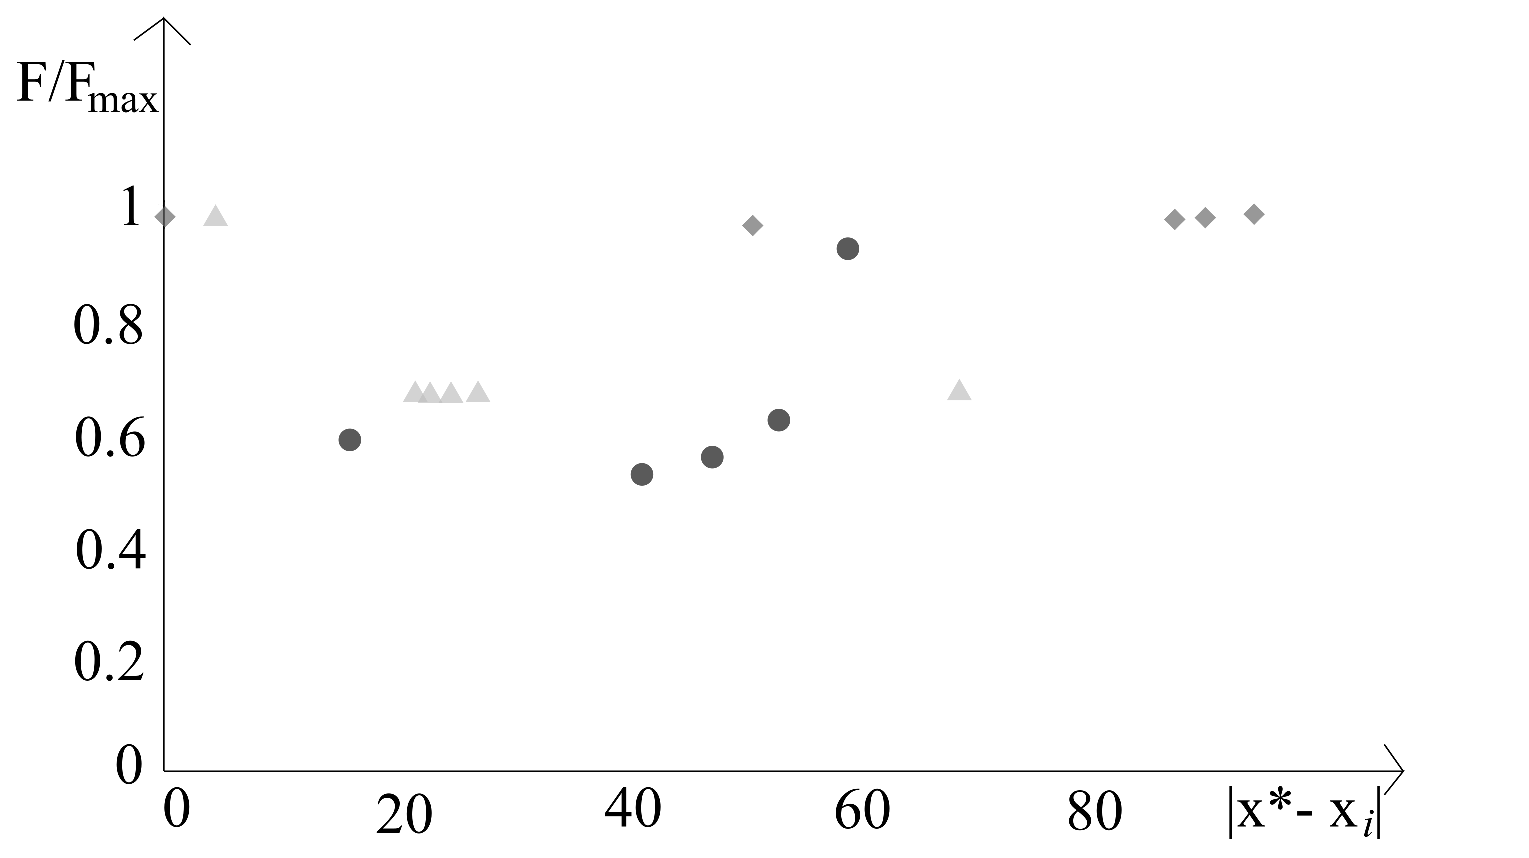
\includegraphics[width=0.9\linewidth]{fit_dist.eps}  \\ а) }
    \end{minipage}
    \begin{minipage}[h]{0.8\linewidth}
            \center{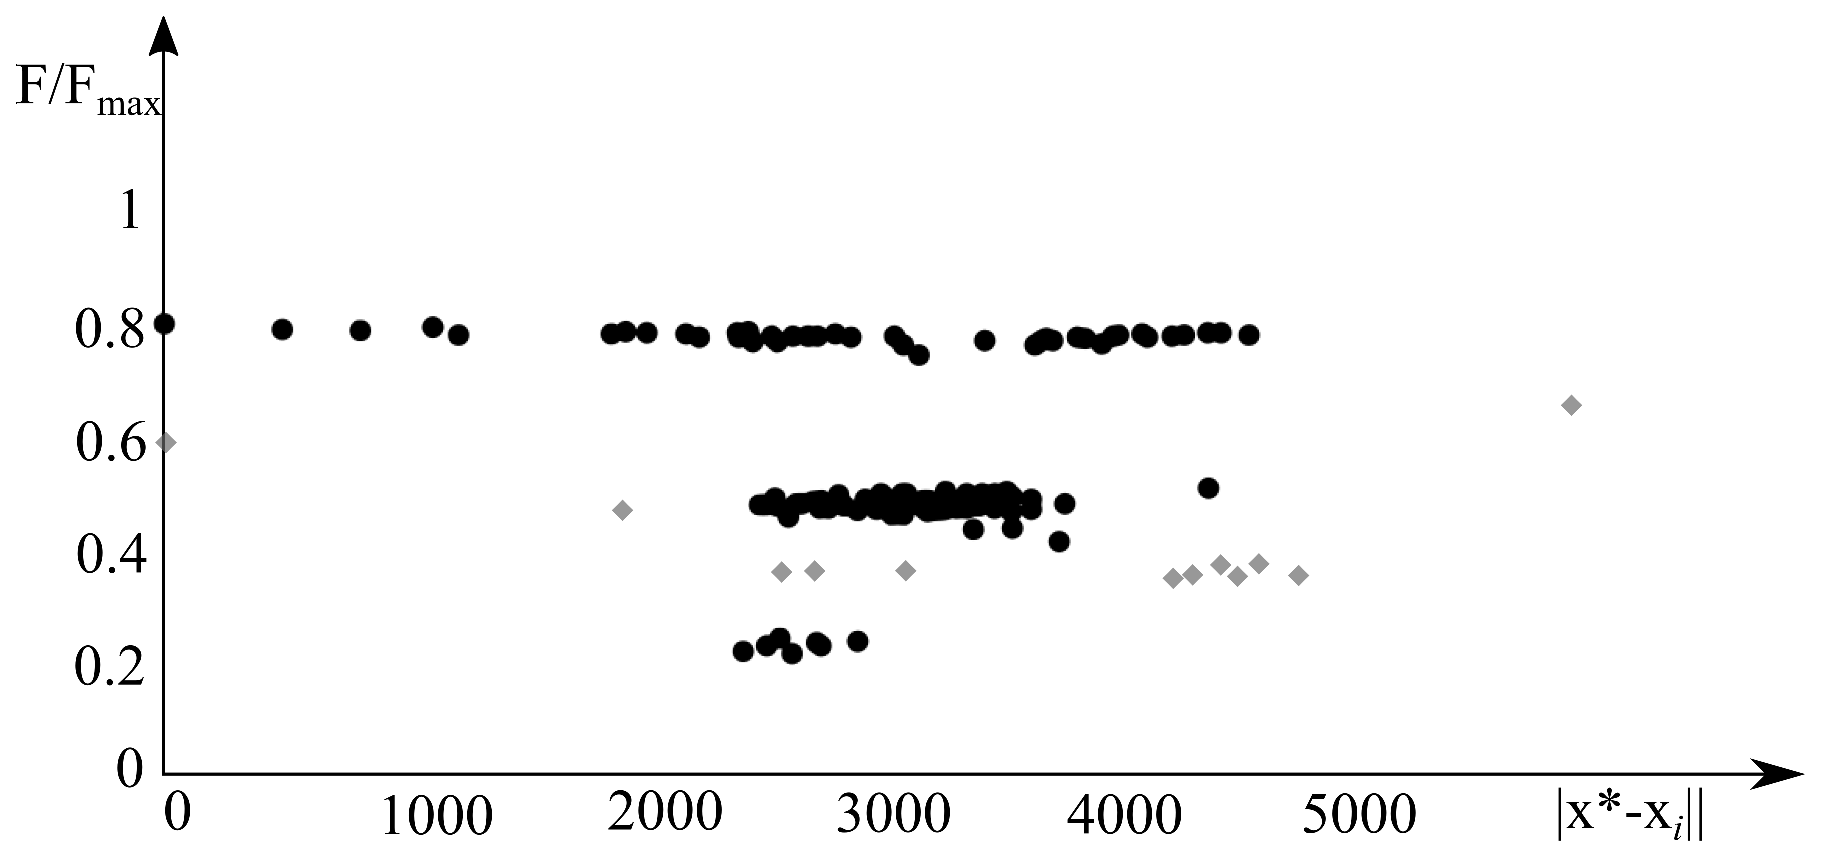
\includegraphics[width=0.9\linewidth]{fit_dist_2x2.eps}  \\ б) }
    \end{minipage}
    \vspace{0.7em}
    \caption{Структура множества найденных решений для задач ШВИ, ШВД, СВД (а) и СВД' (б)}
    \label{ris:fit_dist}
\end{figure}

Для оценки общего числа локальных оптимумов использовался метод переписи Шнабеля. Данный метод имеет применение в экологии и заключается в
выводе статистических оценок численности популяции на основе числа особей, помеченных в результате эксперимента, из популяции с неизменным
составом, где каждая особь имеет константную вероятность отлова. В~\cite{eremeev:confidence} предлагается адаптация такого метода для оценки числа локальных оптимумов. В таблице~\ref{tab:structure} приводится статистика по числу различных точек остановки (в пределах заданной точности) процедуры мультистарта в течение 1000~с. процессорного времени. Для каждого решения была применена процедура линеаризации задачи и проверки необходимых условий локальной оптимальности. Приемлемыми считались отличия целевой функции линеаризованной задачи от значения целевой функции, найденного градиентным методом менее чем на 1\%. Здесь {$M$} - число выполненных запусков за отведенное время, $M_{ne}$ - число групп решений, отличающихся не более чем на 10\% по каждой из координат, {$M_{f}$} - число групп значений целевой функции у таких неэквивалентных решений (с точностью до 10\%, приведенных в таблице~\ref{tab:results}). {$M_{y\approx0}$} - число групп решений, для которых были выполнены необходимые условия локальной оптимальности. $\mathcal{B}$ и $\mathcal{L}$ - оценка нижней границы и оценка максимального правдоподобия числа локальных оптимумов, рассчитанные по методу переписи Шнабеля. Доверительная вероятность для данного метода была выбрана равной 95\%. Оценки для числа решений с различными значениями целевой функции обозначены $\mathcal{B}_{M_f}$ и $\mathcal{L}_{M_f}$. Оценки для числа решений, для которых были выполнены необходимые условия локальной оптимальности, обозначены $\mathcal{B}_{M_{y\approx0}}$ и $\mathcal{L}_{M_{y\approx0}}$.

Как видно из таблицы, во всех экспериментах в некоторых запусках были найдены неразличимые с практической точки зрения решения.

На рис.~\ref{ris:fit_dist} приведены диаграммы локальных оптимумов, где по оси ординат отложены значения целевой функции, а по оси
абсцисс - расстояние до лучшего известного решения. В случае а) точками обозначены результаты для кольцевых решеток, состоящих из 8 излучателей, ромбами - для кольцевых решеток, состоящих из 16 излучателей, пятиугольниками - для СВД~3x3. В случае б) точками обозначены результаты для СВД'~2x2, ромбами - для СВД'~3x3. Диаграмма показывает, что значения, соответствующие одному и тому же значению целевой функции, могут находиться достаточно далеко друг от друга, что позволяет сделать предположение о наличии неучтенных симметрий задачи (о множестве линейных симметрий задачи см. в~\cite{yurkov:symmetry}).
Наличие большого количества решений, соответствующих одному и тому же значению целевой функции, приводит нас к исследованию групп симметрий. В~\cite{yurkov:symmetry} показано, что любой элемент группы непрерывных симметрий задачи~\ref{eq:task3} может быть описан в виде~\ref{eq:sunexp}.
\begin{equation}
\label{eq:sunexp}
Q=e^{\sum\limits_n a_n G_n} \, .
\end{equation}
где $a_n$ - вещественные числа, $G_n$ - генераторы. В качестве генераторов можно выбрать косо-симметричные матрицы, которые содержат над главной диагональю один единичный элемент, симметричный ему противоположный элемент и остальные нули.
Введем матрицу: $ {\textbf{H}}_{\Sigma} = \sum_{i} \textbf{H}_i,$ которая может быть представлена в виде конгруэнтного преобразования диагональной матрицы $D$:
$${\textbf{H}}_{\Sigma} = S^TDS,$$
Нахождение непрерывных групп симметрий сводится к решению задачи~\ref{eq:commutat2}.

\begin{equation}
\label{eq:commutat2}
\left\{
\begin{array}{l}
\displaystyle
\tilde{\textbf{H}}_i \left(\sum\limits_na_nG_n\right) =
\left(\sum\limits_na_nG_n\right)\tilde{\textbf{H}}_i \, , \\ \\
\displaystyle
\tilde{\textbf{G}} \left(\sum\limits_na_nG_n\right) = \left(\sum\limits_na_nG_n\right)\tilde{\textbf{G}} \, .
\end{array}
\right.
\end{equation}

\begin{equation}
\tilde{\textbf{G}}=\left(S^{-1}\right)^T \textbf{A} S^{-1} \, , \qquad
\tilde{\textbf{B}_i}=\left(S^{-1}\right)^T \textbf{B}_i S^{-1} \, , \ i=1,\dots,M.
\end{equation}

Вычислительный эксперимент состоит из следующих этапов:
\begin{enumerate}
  \item Обработка. На этом этапе возможная неточность данных нивелируется усреднением симметричных компонент матриц (матрицы $\textbf{G}$ и $\textbf{H}$ должны быть симметричны).
  \item %Normalization of matrices $B_i$.
  Преобразование $ {\textbf{H}}_{\Sigma} = \sum_{i} \textbf{H}_i$ к канонической форме используя метод Лагранжа для вычисления матриц~$S$ и $S^{-1} $.
  \item Применение метода Гаусса к системе линейных~(\ref{eq:commutat2}) для вычисления генераторов~$\hat{G}_n$.
\end{enumerate}

%\subsection{Optimization of the Excitation of Antenna Arrays}

Описанная процедура нахождения непрерывных групп симметрий применяется к примерам, описанным во второй главе. Для всех рассмотренных задач было выявлено только наличие фазовой симметрии. Возможно, множественность решений объясняется наличием дискретных симметрий. Выявление дискретных симметрий является объектом дальнейших исследований.

Как было показано выше, градиентный метод может предоставить решение, не являющийся локальным оптимумом, если целевая функция слабо изменяется в окрестности текущей точки. Алгоритм дифференциальной эволюции не подвержен такому поведению.
Эксперименты показывают, что в целом эволюция популяции соответствует динамике случайного облака точек, движущегося как целое вдоль рельефа оптимизируемой функции, повторяя его характерные особенности. В случае попадания в овраг «облако» принимает форму этого оврага и распределение точек становится таким, что математическое ожидание разности двух случайных векторов оказывается направленным вдоль длинной стороны оврага. Это обеспечивает быстрое движение вдоль узких вытянутых оврагов, тогда как для градиентных методов в аналогичных условиях характерно колебательная динамика «от стенки к стенке». Приведенные эвристические соображения иллюстрируют наиболее важную и привлекательную особенность алгоритма ДЭ — способность динамически моделировать особенности рельефа оптимизируемой функции. Именно этим объясняется замечательная способность алгоритма быстро проходить сложные овраги, обеспечивая эффективность даже в случае сложного рельефа.

Кратко опишем идею алгоритма ДЭ. В начале происходит генерация популяции. Если нет дополнительной информации, такая популяция особи популяции генерируются случайным образом с равномерным распределением. Затем, пока все особи не сойдутся в одной точке, каждая особь подвергается мутации путем присваивания ей признаков другой особи. Процедура, определяющая, в какой степени признаки других особей участвуют в эволюции конкретной особи является параметром алгоритма. Далее происходит сравнение значений целевой функции мутировавшей особи со значением целевой функции исходной особи. Выживает особь с лучшим значением целевой функции.

Данный алгоритм хорошо поддается модификации для запуска в параллельных потоках. В этом случае, на очередной итерации алгоритма выбирается некоторый набор особей, эволюция каждой из которых на данной итерации происходит независимо от эволюции другой. В данной работе был предложен вариант реализации алгоритма дифференциальной эволюции, адаптированный для запуска на графическом устройстве. Использование алгоритма ДЭ позволило достичь решения с целевой функцией $\tilde{F} = 253$ для задачи СВД'~2x2.

\underline{\textbf{Третья глава}} посвящена исследованию ФАР в различных условиях.

На практике использование высоко симметричных ФАР вызывает особый интерес из следующих соображений: измерение матрицы сопротивлений является тривиальной задачей, в то время как измерение парциальных полей требует большое количество приемников для всех возможных направлений излучения. Использование высокосимметричных ФАР позволяет выполнить расчеты для одного направления и затем легко адаптировать их для других симметричных направлений. Другой особенностью, влияющей на результаты моделирования является наличие потерь в земле (см.~\cite{yurkov:groundloss}). Чтобы ослабить этот эффект, антенные системы с противовесами подняты над землей на 2 м.

В данной главе мы изучаем, как изменяется общий коэффициент усиления с ростом радиочастоты и плотности системы противовесов. Общий коэффициент усиления является суммой частичных коэффициентов усиления в  двух ортогональных поляризациях. Плотность системы противовесов определяется числом продольных и поперечных проводов, относящихся к одному и тому же излучателю. Частота изменяется от 5 до 30 МГц. Вычисления производились на решетках ШВИ, состоящих из 8 излучателей. Для расчета матрицы сопротивлений и матрицы излучений использовался пакет моделирования антенных систем NEC2~\cite{bruke:nec2}.

Для проведения вычислительного эксперимента использовался решатель BARON в пакете GAMS, поскольку, в основном он деонстрирует лучшие результаты по сравнению с градиентным подъемом. Результаты оптимизации направленности решетки сравниваются с коэффициентом усиления одиночного излучателя, установленного в центре такой же системы противовесов. Плотность системы противовесов обозначается в формате $long:trans$, где $long$ - число продольных проводов, относящихся к одному излучателю, а $trans$ - поперечных. Высота каждого ШВИ - 15м. В качестве направления оптимизации выбирается $70^{\circ}$ полярного угла и $45^{\circ}$ азимутального угла в сферических координатах.

\begin{figure}
\center{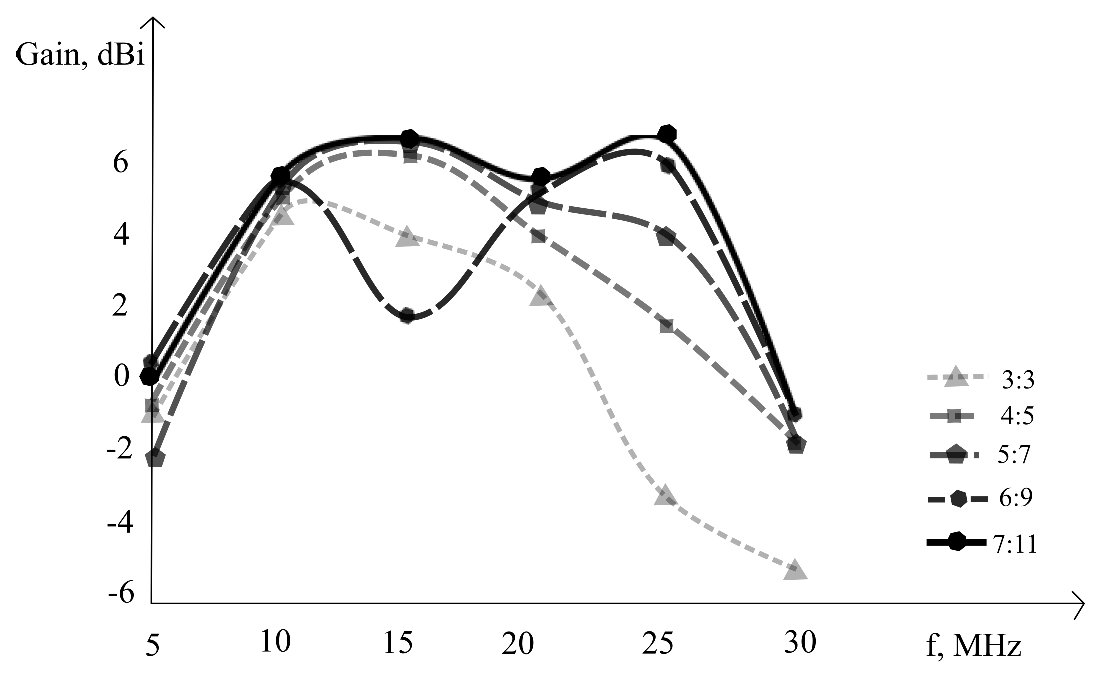
\includegraphics[width=0.8\linewidth]{ring_f__paa_gains.eps}}
\caption{Зависимость от частоты общего коэффициента усиления ФАР при оптимизации в направлении 70:45}
\label{ris:paa_gains}
\end{figure}

На рис.~\ref{ris:paa_gains} показано, как изменяется коэффициент усиления с ростом радиочастоты. Мы можем наблюдать, что при значениях частоты 5 и 30 МГц решетка оптимизируется довольно плохо. Также можно увидеть, что, в основном, увеличение плотности системы противовесов приводит к росту коэффициента усиления. Единственное исключение - решетка с плотностью системы противовесов $6:9$ на частоте 15МГц, где наблюдается неожиданное падение коэффициента усиления. Такое поведение может быть объяснено тем, что BARON не достиг глобалного оптимума.

\begin{figure}
\center{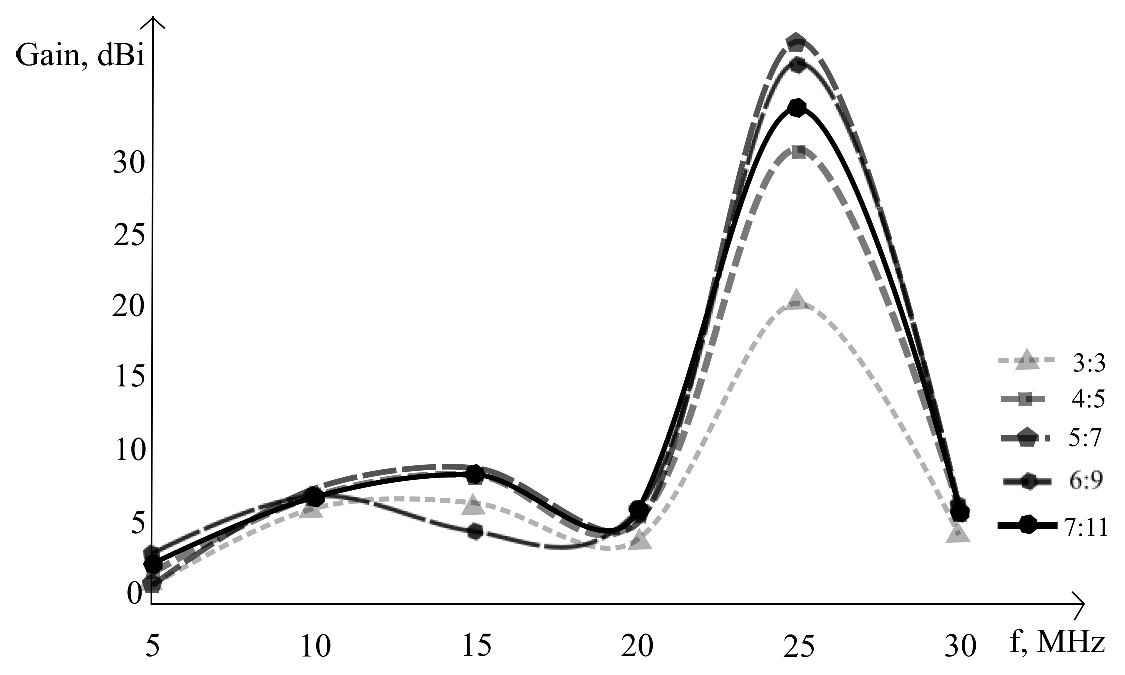
\includegraphics[width=0.8\linewidth]{ring_f_gains.eps}}
\caption{Сравнение коэффициентов усиления ФАР и одиночного излучателя}
\label{ris:all_gains}
\end{figure}

На рис.~\ref{ris:all_gains} показано, как изменяется разница коэффициентов усиления ФАР и одиночного излучателя с ростом частоты. Заметным результатом здесь является то, что на частоте 25МГц усиление ФАР существенно больше усиления одиночного излучателя. Объяснение этого эфффекта будет приведено далее при сравнении диаграмм направленности. При 5МГц усиление ФАР существенно не превосходит усиление одиночного излучателя, однако, уже на 10МГц разница возрастает до 7.53дБ. Даже при 30МГц, где ФАР не оптимизируется хорошо, разница с одиночным излучателем составляет 6.63дБ в лучшем случае и 4.84дБ в худшем.

\begin{figure}
\begin{minipage}[h]{0.49\linewidth}
\center{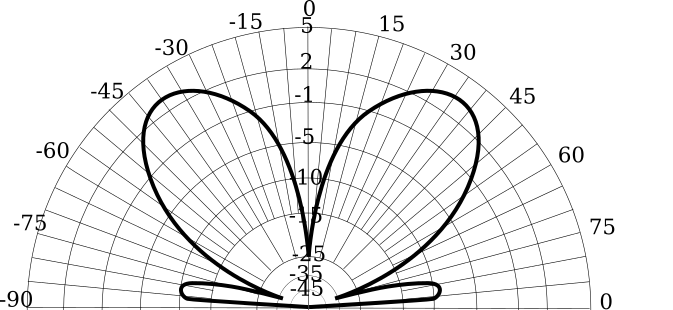
\includegraphics[width=1\linewidth]{r8_1_25_5x7.png} \\ а)}
\end{minipage}
\hfill
\begin{minipage}[h]{0.49\linewidth}
\center{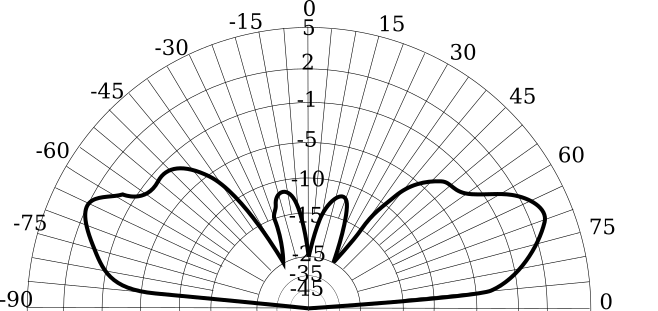
\includegraphics[width=1\linewidth]{r8_25_5x7.png} \\ б)}
\end{minipage}
\caption{Вертикальный план диаграммы направленности одиночного излучателя (а) и ФАР 5:7 (б) при 25МГц}
\label{ris:f25mhs}
\end{figure}

Интересный результат наблюдается при 25МГц (см~Рис.~\ref{ris:f25mhs}), где усиление ФАР существенно больше усиления одиночного излучателя. Сравнение их диаграмм направленности показывает, что одиночный излучатель довольно плохо излучает в направлении оптимизации, тогда как ФАР имеет максимум излучения в этом направлении. Предположительно, такой эффект был получен вследствие учета взаимного влияния. Согласно~(\ref{eq:A}), если пренебречь взаимным влиянием излучателей, плотность мощности $F$ будет максимальна тогда, когда комплексные амплитуды парциальных полей будут синфазны. Для проверки гипотезы о необходимости учета взаимного влияния в данной работе производилось сравнение диаграмм направленности решеток разных конфигураций после математической оптимизации их направленности в заданном направлении согласно модели~(\ref{eq:task3}) с соответствующими диаграммами одиночного излучателя и со случаем фазирования решетки без учета взаимного влияния (далее – простое фазирование).

Для проведения вычислительного эксперимента использовался решатель BARON в пакете GAMS, поскольку, как правило, он обеспечивает бо́льшую точность решений по сравнению с градиентным подъемом [A1]. Высота каждого ШВИ равна 15~м. Длина плеча симметричных излучателей также равна 15~м. Направление оптимизации по умолчанию было установлено на $70^{\circ}$ полярного угла и $45^{\circ}$ азимутального угла в сферических координатах. Для некоторых экспериментов было проведено дополнительное исследование при $85^{\circ}$ полярного угла.


\begin{figure}
    \begin{minipage}[h]{0.49\linewidth}
        \center{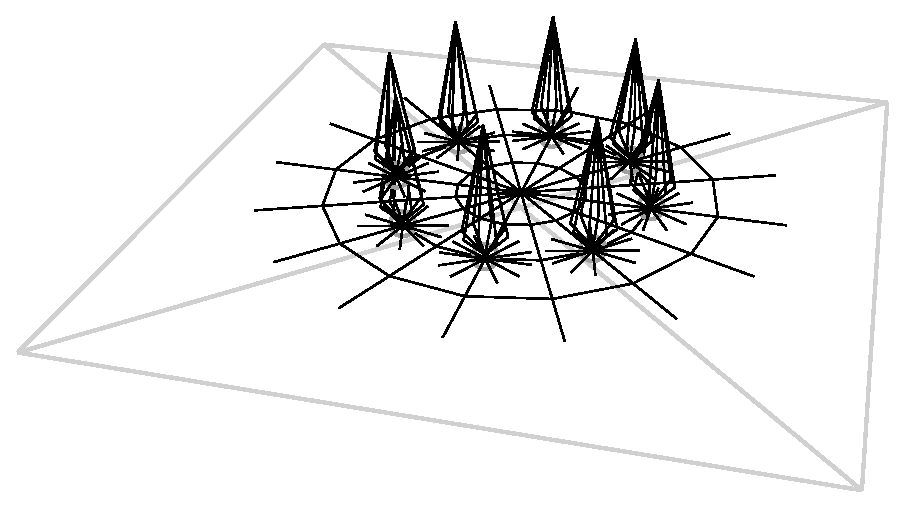
\includegraphics[width=0.8\linewidth]{r_bve_w.eps} \\ а)}
    \end{minipage}
    \hfill
    \begin{minipage}[h]{0.49\linewidth}
        \center{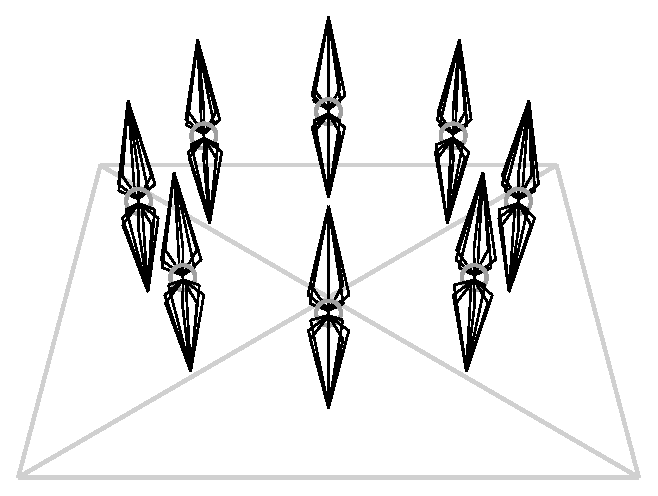
\includegraphics[width=0.6\linewidth]{r_bvd.eps} \\ б)}
    \end{minipage}
    \begin{minipage}[h]{1\linewidth}
        \center{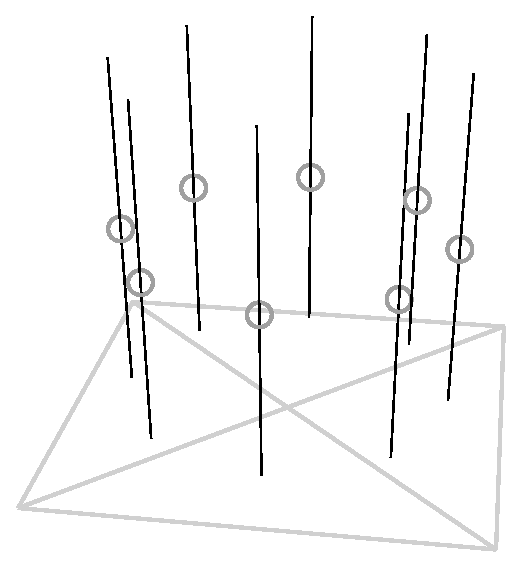
\includegraphics[width=0.25\linewidth]{r_svd.eps} \\ в)}
    \end{minipage}
    \caption{ФАР кольцевой структуры: ШВИ (а) ШВД (б) и СВД (в)}
    \label{pic:r_paas}
\end{figure}

Для решеток ШВИ~(см.~Рис.~\ref{pic:r_paas},~а.) производилось сравнение диаграмм направленности при варьировании расстояния центра излучателя до центра решетки (от~7 до 80~м.), длины радиальных противовесов (от 3 до 20 м.) и присутствия или отсутствия общей системы противовесов. Диаграммы направленности при этом имели различную форму, однако, качественно различие между коэффициентами усиления всегда сохранялось: результат оптимизации не дает значимого преимущества перед простым фазированием.

Для ШВД~(см.~Рис.~\ref{pic:r_paas},~б.) производилось исследование диаграмм направленности при варьировании расстояния центра излучателя до центра решетки от~5 до 50~м. В большинстве случаев, использование решения задачи математического программирования не давало существенного преимущества перед простым фазированием. Тем не менее, при расстоянии между центром излучателя и центром решетки равным 20~м. это различие составило около 4~дБ~(см.~Рис.~\ref{pic:r_bvd_result}).

\begin{figure}
\begin{minipage}[h]{0.49\linewidth}
\center{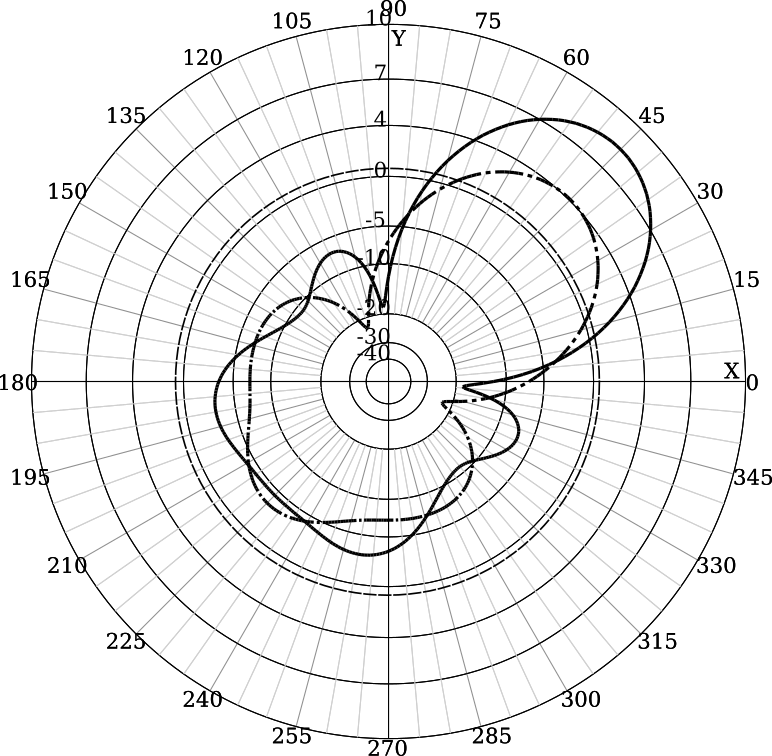
\includegraphics[width=1\linewidth]{r_bvd_20_results_h.png} \\ а)}
\end{minipage}
\hfill
\begin{minipage}[h]{0.49\linewidth}
\center{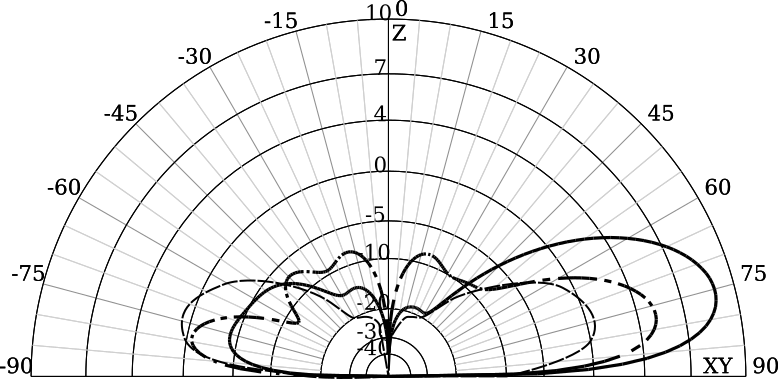
\includegraphics[width=1\linewidth]{r_bvd_20_results_v.png} \\ б)}
\end{minipage}
\caption{Горизонтальный (а) и вертикальный (б) план диаграммы направленности ШВД при расстоянии от центра излучателя до центра решетки 20 м. Пунктирной линией обозначено усиление одиночного излучателя, штрихпунктирной – простое фазирование, сплошной – решение задачи мат. программирования.}
\label{pic:r_bvd_result}
\end{figure}

Аналогичные результаты были получены и для решетки~(см.~Рис.~\ref{pic:r_paas},~в.). При оптимизации в направлении полярного угла равном $70^{\circ}$ при варьировании расстояния от центра излучателя до центра решетки от~35 до 37~м. разница между коэффициентом усиления решения задачи математического программирования и усилением простого фазирования также достигала 4~дБ.  При оптимизации в направлении полярного угла равном $85^{\circ}$ при варьировании расстояния от центра излучателя до центра решетки от 25 до 29~м. эта разница достигала 5~дБ.

В \underline{\textbf{четвертой главе}} приведено разработанного программного комплекса. Для проведения вычислительных экспериментов был разработан интерпретатор <<Expi>> и его графическая оболочка <<ExpiIDE>>.

Формат языка <<Expi>> позволяет в декларативной форме объявлять правила построения моделей и задавать параметры запуска экспериментов.
В языке <<Expi>> предоставлены возможности моделировать конфигурации проводников в зависимости от динамических параметров, объединять их в группы и применять к ним геометрические преобразования. Также имеется возможность экспорта определенных конфигураций в формат NEC. Отдельно следует отметить возможность языка выполнять серии вычислительных экспериментов. В <<Expi>> уже встроен интерфейс для работы с пакетом GAMS, а также имеется возможность интеграции любого пользовательского пакета.

Графическая оболочка <<ExpiIDE>> представляет собой файловый инспектор с возможностью редактировать и запускать файлы экспериментов exp, просматривать и экспортировать диаграммы направленности и геометрию антенных систем.

\FloatBarrier
\pdfbookmark{Заключение}{conclusion}                                  % Закладка pdf
В \underline{\textbf{заключении}} приведены основные результаты работы, которые заключаются в следующем:
%% Согласно ГОСТ Р 7.0.11-2011:
%% 5.3.3 В заключении диссертации излагают итоги выполненного исследования, рекомендации, перспективы дальнейшей разработки темы.
%% 9.2.3 В заключении автореферата диссертации излагают итоги данного исследования, рекомендации и перспективы дальнейшей разработки темы.
\begin{enumerate}
  \item В текущей работе была рассмотрена постановка задачи оптимизации направленности излучения антенной системы, представленной в виде регулярной решетки излучателей. Для данной задачи была разработана модель квадратичного программирования в вещественных числах. Произведено сравнение результатов разработанных алгоритмов в вычислительном эксперименте.
  \item Проведены вычислительные эксперименты, выявляющие наличие непрерывных групп симметрий допустимых решений. Для всех рассмотренных задач выявлено наличие только фазовой симметрии.
  \item В рамках данного исследования было выявлено наличие ситуаций, в которых коэффициент усиления, соответствующий решению задачи математического программирования, имеет существенное преимущество перед коэффициентом усиления простого фазирования. Выявлено, что, при оптимизации направленности ФАР КВ диапазона целесообразны расчеты с учетом взаимного влияния излучателей.
  \item Для генерации тестовых примеров, автоматизации вычислительных экспериментов и визуализации их результатов были разработаны интерпретатор <<Expi>> и его графическая оболочка <<ExpiIDE>>.
\end{enumerate}

    % Введение
\ifnumequal{\value{contnumfig}}{1}{\counterwithout{figure}{chapter}
}{\counterwithin{figure}{chapter}}
\ifnumequal{\value{contnumtab}}{1}{\counterwithout{table}{chapter}
}{\counterwithin{table}{chapter}}
\chapter{Задача оптимизации направленности фазированных антенных решеток}\label{ch:ch1}

\section{Основные понятия}

Как и в работах~\cite{yurkov:groundloss,yurkov:knd} мы изучаем антенные решетки КВ диапазона, состоящие из широкополосных вертикальных
излучателей (ШВИ), см. Рис.~\ref{ris:bve_bvd}~a) и широкополосных вертикальных диполей (ШВД), см. Рис.~\ref{ris:bve_bvd}~б). Кроме того, в
рассмотрение включены решетки симметричных вертикальных диполей (СВД), см. Рис.~\ref{ris:bve_bvd}~в) и решетки ШВИ кольцевой структуры, см. Рис.~\ref{ris:bve_bvd}~г).

Каждый ШВИ состоит из 8 проводов, которые составляют ``каплеобразный'' вертикальный излучатель, обеспеченный системой противовесов.
Система противовесов каждого излучателя состоит из 6 проводов, расположенных параллельно земле. ШВД спроектирован аналогично ШВИ с той
разницей, что вместо системы противовесов подключен другой ``каплеобразный'' вертикальный излучатель, направленный в противоположную сторону. СВД являются диполями стандартной конфигурации, то есть, представляют собой прямолинейный проводник, длина которого много
больше его радиуса, питаемый от генератора посередине. Решетки ШВИ кольцевой структуры представляют собой несколько ``каплеобразных''
вертикальных излучателей, расположенных по кругу с некоторым фиксированным шагом. Система противовесов для такой решетки состоит из
радиальных проводников, причем через каждый излучатель проходит один такой проводник. Кроме того, система противовесов состоит из поперечных проводников, соединяющих соседние излучали, а также параллельных ему проводников в данном секторе. В принципе, в рассмотрение могут быть включены излучатели, спроектированные любым другим образом, если для них предоставлены соответствующие входные данные задачи оптимизации ФАР. Здесь под входными данными понимаются матрицы компонент полей и матрицы проводимости, которые можно получить с помощью некоторой программы моделирования антенн.

\begin{figure}
    \begin{minipage}[h]{0.49\linewidth}
        \center{\includegraphics[width=1\linewidth]{2x2bvm.eps} \\ а)}
    \end{minipage}
    \hfill
    \begin{minipage}[h]{0.49\linewidth}
        \center{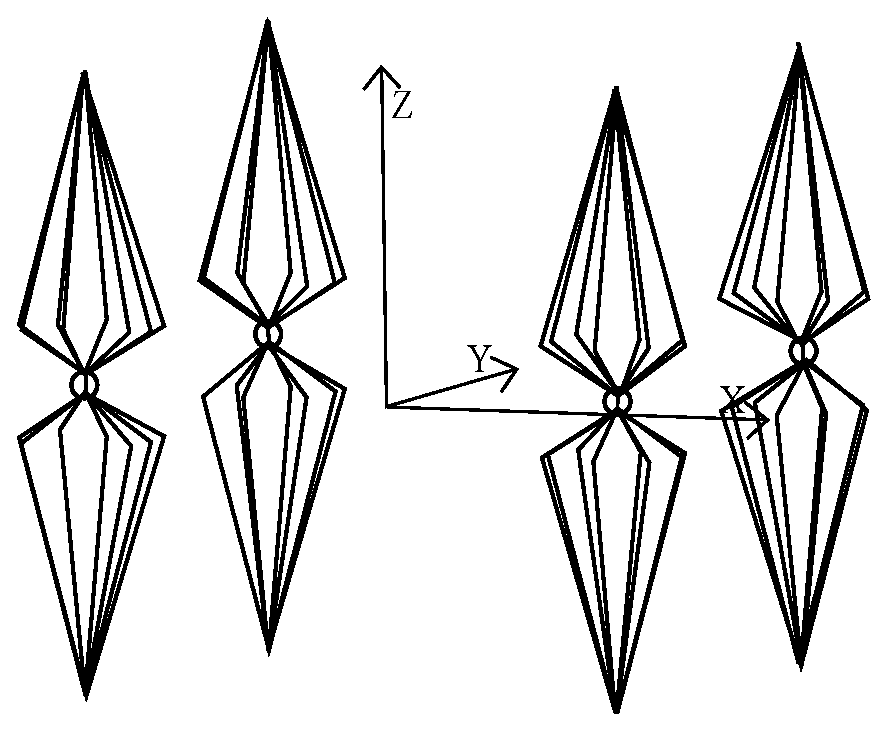
\includegraphics[width=0.6\linewidth]{2x2bvd.eps} \\ б)}
    \end{minipage}
    \begin{minipage}[h]{0.49\linewidth}
        \center{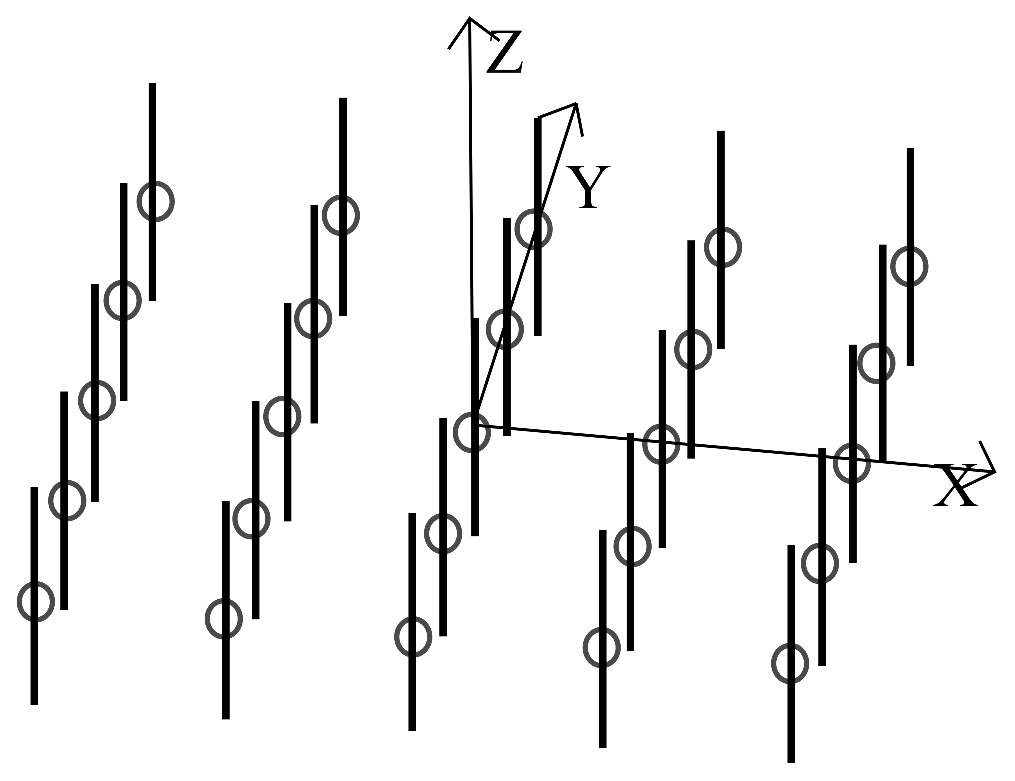
\includegraphics[width=0.6\linewidth]{5x5SVD.eps} \\ в)}
    \end{minipage}
    \hfill
    \begin{minipage}[h]{0.49\linewidth}
        \center{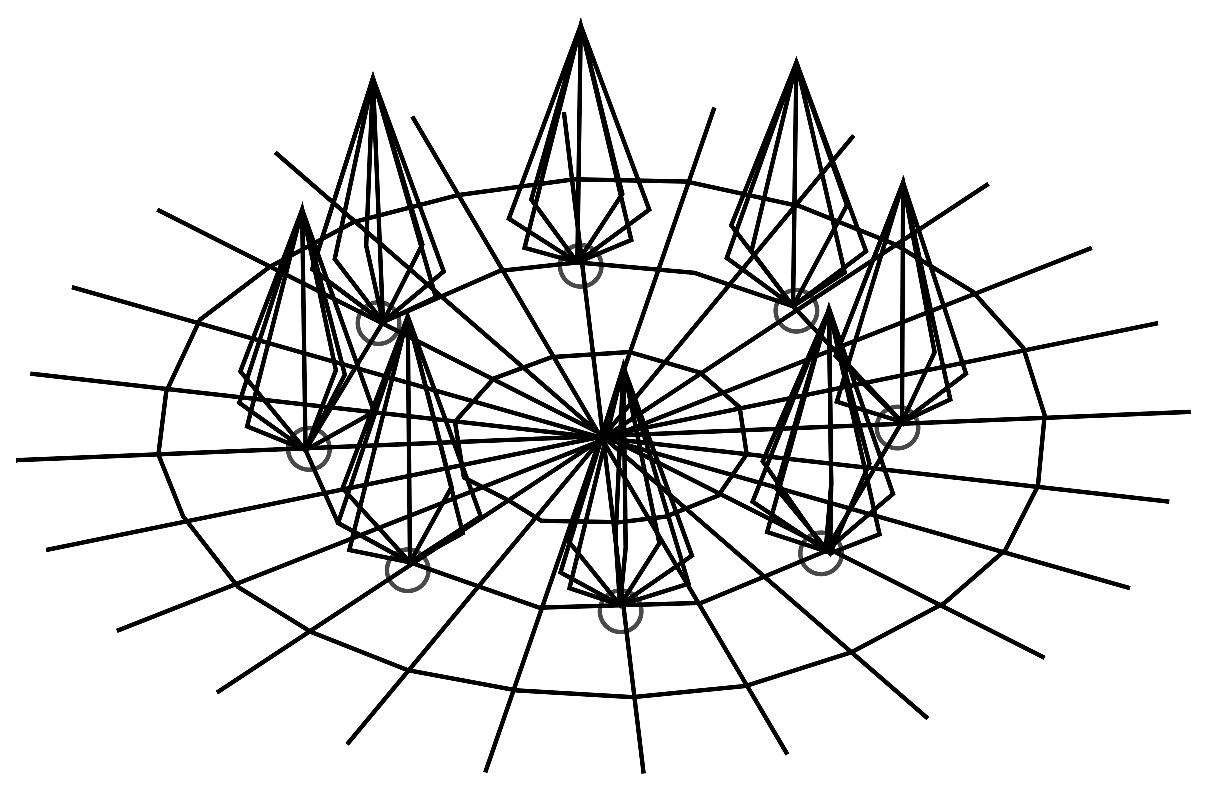
\includegraphics[width=0.9\linewidth]{r8.eps} \\ г)}
    \end{minipage}
    \caption{ФАР различных конфигураций}
    \label{ris:bve_bvd}
\end{figure}


\section{Постановка задачи}\label{sec:statement}
Нашей задачей является максимизация излучения антенной решетки в заданном направлении при ограничениях на мощность, подводимую к каждому
излучателю. В терминах комплексных токов, подводимых к излучателям, эта задача сформулирована в работах~\cite{yurkov:farkv,yurkov:knd}.
Пусть $l$ - индекс компоненты вектора направления: $l=1$ для азимутального и $l=2$ для полярного угла. Расстояние до приемника принимается во много раз превышающим размеры ФАР, поэтому индекс $l$ итерирует только эти два значения.
Суммарное электромагнитное поле $f^{(l)}_{\Sigma}$, выраженное в комплексных единицах, вводится как
%
\begin{equation}
    f^{(l)}_{\Sigma} = \sum_{i=1}^{N}I_i \tilde{f}_i^{(l)} \, ,
    \label{eq:sumfield}
\end{equation}
%
где $N$ - число точек питания антенной системы, $I_i$ - комплексный ток в $i$-й точке питания; $\tilde{f}_i^{(l)}$ - парциальное поле, то есть поле, которое излучается при подаче единичного тока на $i$-ю точку питания излучающей системы, в то время, как ток в других точках питания равен нулю. В качестве количественной меры оценки электромагнитного поля используется напряженность электрического поля. Отметим, что из определения парциального поля следует, что $\tilde{f}_i^{(l)}$ имеет размерность поля, нормированного к току. Справедливость выражения~(\ref{eq:sumfield}) следует из линейности уравнений Максвелла (более подробно см.~\cite{yurkov:farkv}). Таким образом, суммарное поле $f^{(l)}_{\Sigma}$ является суперпозицией парциальных полей от каждой точки питания излучающей системы.

Значения $f_i^{(l)}$ и $f^{(l)}_{\Sigma}$ -- функции направления и частоты, которые могут быть вычислены с помощью некоторой программы моделирования антенн (здесь мы используем NEC-2~\cite{bruke:nec2}).

За $\overline{f}$ обозначим комплексное сопряжение к $f$. Как было упомянуто выше, цель -- максимизация направленности излучения. В качестве количественной меры оценки направленности излучения понимается плотность мощности поля в заданном направлении, обозначаемая через $F$. Через компоненты электромагнитного поля величина $F$ выражается по формуле~(\ref{eq:FPrimary})
%
    \begin{equation}
        F = \sum_{l=1}^{2}\overline{f}_{\Sigma}^{(l)}f_{\Sigma}^{(l)}
        \label{eq:FPrimary}
    \end{equation}
%
и является целевой функцией задачи. При максимизации $F$ необходимо учитывать ограничения на активную мощность, которую способны выдавать усилители, питающие антенную систему. В силу закона Ома такие ограничения могут быть выражены в терминах только токов или только напряжений. Чтобы найти мощность $i$-го источника, вводятся соответствующие комплексные напряжения~$U_i$ следующим образом:
%
    \begin{equation}
        I_i = \sum_{j=1}^{N}y_{ij}U_j \, ,
        \label{eq:om}
    \end{equation}
%
где $y_{ij}$ -- элементы матрицы проводимостей $\textbf{Y} = (y_{ij})$, имеющей размерность $N \times N$.

В некоторых случаях более удобно использовать матричную нотацию. В рамках данной нотации мы вводим вектор-столбец токов $\textbf{i}$ и вектор-столбец напряжений $\textbf{u}$, состоящие из $N$ элементов. Целевая функция в таком случае формулируется следующим образом:
%
    \begin{equation}
        F = \textbf{u}^{+}\textbf{Au} \, ,
        \label{eq:F}
    \end{equation}
%
где верхний индекс $+$ означает эрмитово сопряжение, $A = (a_{ij})$,
%
     \begin{equation}
        a_{ij} = \sum_{l=1}^2\overline{f}_{i}^{(l)}f_{j}^{(l)}
        \label{eq:A} \, .
    \end{equation}
%
Соответственно, соотношение между токами и напряжениями записывается следующим образом:
%
    \begin{equation}
    \textbf{i}=\textbf{Y}\textbf{u} .
    \end{equation}
%

Существуют различные формы ограничений, которые соответствуют различным антенным системам. Например, можно ограничить суммарную мощность $P$ по всем точкам питания. В этом случае задача оптимизации формулируется так:
%
     \begin{equation}
        \begin{cases}
           \textbf{u}^{+}\textbf{Au} \rightarrow \max,\\
           \textbf{u}^{+}\textbf{Bu} = 1,
         \end{cases}
         \label{eq:task1}
    \end{equation}
%
где
%
    \begin{equation}
        \textbf{B} = \frac{1}{4P}(\textbf{Y} + \textbf{Y}^{+}).
        \label{eq:B}
    \end{equation}
%
Такая задача может быть решена аналитически~\cite{yurkov:farkv}.

Задача усложняется, когда ограничение на мощность накладывается по каждой точки питания. В этом случае задача формулируется в виде:
%
    \begin{equation}
        \begin{cases}
           \textbf{u}^{+}\textbf{Au} \rightarrow \max,\\
           0 \leq \textbf{u}^{+}\textbf{B}^{(1)}\textbf{u} \leq 1, \\
           ...\\
           0 \leq \textbf{u}^{+}\textbf{B}^{(n)}\textbf{u} \leq 1,\\
           \textbf{u} \in \mathbb{C}^N\\
         \end{cases}
         \label{eq:task2}
    \end{equation}
%
где $\mathbb{C}$ - поле комплексных чисел, $n$ - число точек питания, на которые накладываются ограничения (в общем случае $n$ может быть не равно $N$),
%
    \begin{equation}
        \textbf{B}^{(k)} = \frac{1}{4P_{max}^{(k)}}(\textbf{Y}^{+}\mathcal{P}^{(k)} + \mathcal{P}^{(k)}\textbf{Y}) \, ,
    \end{equation}
%
$P_{max}^{(k)}$ - максимально допустимая мощность в $k$-й точке питания, $\mathcal{P}^{(k)}$ - матрицы-проекторы имеющие единственный ненулевой элемент $\mathcal{P}^{(k)}_{kk}=1$. Матрицы-проекторы имеют размерность $N \times N$.

Как показано в~\cite{yurkov:farkv},
%
\begin{enumerate}
  \item Все матрицы $\textbf{B}^{(k)}$ имеют не больше чем два ненулевых собственных значения. Одно из собственных значений положительно,
  остальные отрицательные или нулевые.
  \item Матрицы $\textbf{A}$ и $\textbf{B}^{(k)}$ эрмитово-самосопряженные, то есть
  $a_{ij} = \overline{a}_{ji}$ для всех $i = \overline{1,N}, j = \overline{1,N}$.
  \item Матрица $\textbf{A}$ положительно полуопределена.
  \item Кроме того, из закона сохранения энергии, что матрица $\textbf{B}_{\sum}:= \sum_{k=1}^{n} \textbf{B}^{(k)}$
  положительно определена, так как суммарная активная мощность, поглощаемая пассивной цепью, не может быть отрицательной либо нулем,
  поскольку, часть энергии обязательно излучится~\cite{yurkov:farkv}.
\end{enumerate}

\section{Методы решения}

В данной работе мы рассматриваем подход к решению задачи максимизации направленности излучения ФАР в заданном направлении при ограничениях, накладываемых на мощность, подаваемую на каждый из излучателей. Такая задача может быть решена только численными методами~\cite{yurkov:farkv}. Для использования градиентного метода задача сводится к задаче безусловной оптимизации методом штрафных функций. Выбор градиентного алгоритма связан с тем, что отыскание даже локального оптимума в задаче невыпуклого квадратичного программирования может представлять собой NP-трудную задачу, и одним из методов, уместных в таких случаях, является градиентный алгоритм~\cite{murty:np}. Согласно~\cite{nesterov:nonconvex}, использование метода сопряженных градиентов для решения данной задачи не будет приводить к существенным улучшениям по сравнению с простым градиентным подъемом. Данное утверждение нашло согласие с результатами предварительных вычислительных экспериментов, проведенных нами для некоторых из рассматриваемых задач.

Для оценки качества результатов градиентного алгоритма производится их сравнение с решениями, полученными с помощью решателя
BARON в пакете GAMS. BARON использует алгоритм ветвей и границ, усиленные различными методами распространения ограничений и локального поиска для уменьшения диапазонов переменных в ходе работы алгоритма~\cite{ryoo:nlp}. Его использование также представляет альтернативный подход к решению данной задачи, но, поскольку BARON является коммерческим решателем, произведение расчетов требует приобретения лицензии, что не всегда приемлемо.

Вообще говоря, при использовании метода градиентного подъема не гарантируется получение глобального оптимума. Приблизиться к глобальному
оптимуму позволяет многократный запуск алгоритма из случайным образом сгенерированных точек. Кроме того, многократный запуск позволяет
оценить количество локальных оптимумов, что является некоторым критерием сложности индивидуальной задачи~\cite{eremeev:confidence}. Анализ структуры локальных оптимумов позволяет также выявить наличие нетривиальных симметрий.

Еще одним эффективным подоходом к решению невыпуклых задач квадратичного программирования являются эволюционные алгоритмы, и, в частности, методы дифференциальной эволюции (ДЭ)~\cite{storn:de,noguchi:de}. Использование методов ДЭ требует больше времени, чем использование градиентного подъема, однако, в отличие от градиентных методов, не требует вычисления производных и не подвержен преждевременному завершению в точках стационарности. Таким образом, методы ДЭ также могут быть применены при исследовании структуры локальных оптимумов задачи невыпуклого квадратичного программирования.

\section{Формулировка задачи в действительных числах} \label{subsec:statement}

Для разработки алгоритма решения задачи удобно переформулировать ее в вещественных числах. Обозначим соответствующие матрицы: $\textbf{G} \in \mathbb{R}^{(2N)^2}$ для целевой функции и $\textbf{H}^{(k)} \in \mathbb{R}^{(2N)^2}; k = \overline{1,n}$ для ограничений. Пусть $\textbf{y} \in \mathbb{C}^N$, $\textbf{A} \in \mathbb{C}^{N^2}$, и пусть $\textbf {x} \in \mathbb{R}^{2N}$ - вектор, где первые $N$
компонент являются вещественными частями соответствующих компонент вектора~$\textbf{y}$, в то время, как остальные компоненты соответствуют мнимым, то есть:
%
    $$
    \textbf{y}_i \in \mathbb{C} \longleftrightarrow (\textbf{x}_i,
    \textbf{x}_{N+i}), \ \textbf{x}_i = Re(\textbf{y}_i), \
    \textbf{x}_{N+i} = Im(\textbf{y}_i) \, i = \overline{1,N}.
    $$
%
Через $\textbf{G} \in \mathbb{R}^{(2N)^2}$ обозначим матрицу следующего вида:
%
    \begin{equation}
        \left( \begin{array}{c | c}
            Re(\textbf{A})& -Im(\textbf{A})\\
            \hline
            Im(\textbf{A})& Re(\textbf{A})\end{array}
        \right) .
    \end{equation}
%
Легко проверить, что
    \begin{equation}
        \left(\begin{array}{c} Re(\textbf{Ay}) \\ Im(\textbf{Ay})\end{array} \right) =
        \textbf{G}\left(\begin{array}{c} Re(\textbf{y}) \\ Im(\textbf{y})\end{array}\right) .
    \end{equation}
%

Из того, что матрица $\textbf{A}$ эрмитово-самосопряженная, следует, что матрица $\textbf{G}$ симметричная. Действительно, так как матрица $\textbf{A}$ эрмитово-самосопряжена, следует симметричность $Re(\textbf{A})$ и кососимметричность $Im(\textbf{A})$. Это значит, что
%
    $$
        \textbf{G}^T = \left( \begin{array}{c | c}
            Re(\textbf{A}) & (Im(\textbf{A}))^T \\
            \hline
            (-Im \textbf{A})^T & Re(\textbf{A}) \end{array}
        \right) = \left( \begin{array}{c | c}
            Re(\textbf{A}) & -Im(\textbf{A}) \\
            \hline
            Im(\textbf{A}) & Re(\textbf{A}) \end{array}
        \right)= \textbf{G} \, .
    $$
%
Таким образом, $\textbf{G}$ является симметрической матрицей. То же самое применимо к матрицам ограничений $\textbf{H}^{(k)} \in \mathbb{R}^{(2N)^2}; k=\overline{1,n}$. В вещественных числах задача~(\ref{eq:task2}) эквивалентна следующей:
    \begin{equation}
        \begin{cases}
           \textbf{x}^{T}\textbf{Gx} \rightarrow \max,\\
           0 \leq \textbf{x}^{T}\textbf{H}^{(1)}\textbf{x} \leq 1,\\
           ...\\
           0 \leq \textbf{x}^{T}\textbf{H}^{(n)}\textbf{x} \leq 1,\\
          \textbf{x} \in \mathbb{R}^{2N}.\\
         \end{cases}
         \label{eq:task3}
    \end{equation}

Задача~(\ref{eq:task3}) имеет целевую функцию, заданную квадратичной формой с положительно полуопределенной матрицей~$\textbf{G}$. Каждое ограничение формулируется квадратичной формой, определенной симметричной матрицей~$\textbf{H}^{(k)}, k=\overline{1,n}$ с двумя парами идентичных собственных значений, два из которых положительны, а другие два отрицательны или равны нулю, все остальные собственные числа равны нулю.

Следует отметить, что задача~(\ref{eq:task2}), сформулированная в комплексных числах, имеет симметрию относительно преобразования $\textbf{u} \to e^{\emph{\textbf{j}}\phi}\textbf{u}$ всех комплексных координат (по произвольному углу~$\phi$). За $\emph{\textbf{j}}$ здесь обозначена мнимая единица. В качестве доказательства рассмотрим некоторую квадратичную форму, определенную матрицей \textbf{M}: $${(\textbf{v}e^{\emph{\textbf{j}}\phi})}^{+}\textbf{M}(\textbf{v}e^{\emph{\textbf{j}}\phi}) =
\sum_{l=1}^{N}\sum_{k=1}^{N}|v_k||v_l|m_{kl}e^{\emph{\textbf{j}}(\phi_l + \phi - \phi_k - \phi)} =$$
$$ = \sum_{l=1}^{N}\sum_{k=1}^{N}|v_k||v_l|m_{kl}e^{\emph{\textbf{j}}(\phi_l - \phi_k)} .$$

Отмеченная симметрия может найти применение для уменьшения размерности области поиска на единицу. Например, фиксируя $Im(y_{N})=0$, что эквивалентно добавлению ограничения $x_{2N}=0$ к задаче~(\ref{eq:task3}).

Глобально-оптимальное решение задачи невыпуклого математического программирования вида (\ref{eq:task3}) может быть найдено методом
ветвей и границ~\cite{horst:global,tawarmalani:global} или с использованием методов DC программирования~\cite{horst:handbook,strekalovsky:global}. Локально-оптимальное решение задачи может быть найдено средствами градиентной оптимизации или методом Ньютона~\cite{himmelblau:nlp}. В случае большой размерности могут быть применены различные метаэвристики~(см.~\cite{eberhart:swarm,storn:de}).

%\section{Другие постановки задачи}
% TODO

\section{Верхняя оценка нормы допустимых решений} \label{subsec:top}

В вычислительных экспериментах бывает полезно ограничить множество допустимых решений задачи шаром или параллелепипедом, так как это позволяет более обоснованно выбрать начальное решение для итерационных методов с мультистартом или сократить перебор в методе ветвей и границ.

Кроме того, можно оценить множество допустимых решений в терминах евклидова расстояния до начала координат. Отметим, что если $\textbf{x}$ удовлетворяет всем ограничениям задачи~(\ref{eq:task3}), то
$$
\min\{\textbf{z}^T \textbf{H}_{\sum} \textbf{z} \ : \ \textbf{z}\in
\mathbb{R}^{2N}, \ ||\textbf{z}|| =1\} = \lambda_{\min},
$$
(см. например~\cite{horn:matrix}, глава~1, \S~1.0.2), мы получаем
$$
\textbf{x}^T \textbf{H}_{\sum} \textbf{x} \ge ||\textbf{x}||^2
\lambda_{\min}\ \
$$
и
\begin{equation} \label{eqn:bound}
||\textbf{x}||\le \sqrt{\frac{N}{\lambda_{\min}}}.
\end{equation}

\section{Масштабирование произвольного решения в допустимую область} \label{sec:scaling}

Для рассматриваемой задачи существует преобразование, позволяющее привести к допустимой области решение $\textbf{x}$, которое нарушает только ограничивающие неравенства задачи~(\ref{eq:task3}) вида $\textbf{x}^{T}\textbf{H}^{(k)}\textbf{x} \leq 1$:

\begin{equation}
    \textbf{x}': =\alpha(\textbf{x})^{-1/2} \textbf{x} ,
    \label{eq:scale}
\end{equation}
где $\alpha(\textbf{x}):=\max_{k=\overline{1,n}} \textbf{x}^T \textbf{H}^{(k)}\textbf{x}$. Поскольку как целевая функция, так и ограничения представлены квадратичными формами, применение такой операции приведет к пропорциональному уменьшению в~$\alpha(\textbf{x})$ раз значений каждой из квадратичных форм. Другими словами, если в некоторой точке $\textbf{x}$ значения каждой из квадратичных форм, задающих ограничения, больше 0, причем значения некоторых из них больше 1, то по формуле (\ref{eq:scale}) можно определить множитель, умножение которого на вектор $\textbf{x}$ ведет к тому, что наибольшее из значений квадратичных форм, задающих ограничения, будет равно 1. Данная процедура применяется для выбора начального решения, а также для масштабирования итогового решения.

Результаты данного раздела были представлены в~\cite{tyu:opta,tyu:daor,tyu:fmh}. 
\chapter{Алгоритм дифференциальной эволюции для задачи оптимизации фазированных антенных решеток}\label{sec:radio}

\section{Обзор}
Эволюционные алгоритмы~(ЭА) — один из наиболее широко используемых методов решения сложных задач оптимизации. Несколько вариантов этих стратегий были разработаны и применены во многих областях, таких как наука, экономика и инженерия. Среди них дифференциальная эволюция~(ДЭ)~\cite{storn:de} — одна из наиболее эффективных стратегий непрерывной оптимизации. Более того, ДЭ была признана стратегией-победителем нескольких конкурсов по оптимизации~\cite{das:de}. Подобно другим EA, DE вдохновлен естественным процессом эволюции и включает в себя применение мутаций, рекомбинаций и селекции. Основная особенность метода de заключается в том, что он учитывает различия среди векторов, присутствующих в популяции, для изучения пространства поиска. В этом смысле он похож на оптимизаторы Nelder-Mead~\cite{nelder:simplex} и Controlled Random Search~(CRS)~\cite{price:global}.

ДЭ -- стохастический алгоритм на основе популяции, поэтому он итеративно выводит несколько наборов решений-кандидатов. В ДЭ такие решения-кандидаты обычно называются векторами. В базовом варианте ДЭ для каждого члена популяции~(их называют целевыми векторами) создается новый мутантный вектор. Затем мутантный вектор комбинируют с целевым вектором для создания пробного вектора. Наконец, применяется фаза селекции для выбора выживших. Таким образом, несколько поколений эволюционируют, пока не будет достигнут критерий остановки. В поколении $G$ i-й вектор популяции обозначается как $\textbf{X}_{i,G} = [x_{1,i,G}, x_{2,i,G}, ..., x_{D,i,G}]$. Ниже приведены более подробные сведения о каждой фазе ДЭ.

Эксперименты показывают, что в целом эволюция популяции соответствует динамике случайного облака точек, движущегося как целое вдоль рельефа оптимизируемой функции, повторяя его характерные особенности. В случае попадания в овраг <<облако>> принимает форму этого оврага и распределение точек становится таким, что математическое ожидание разности двух случайных векторов оказывается направленным вдоль длинной стороны оврага. Это обеспечивает быстрое движение вдоль узких вытянутых оврагов, тогда как для градиентных методов в аналогичных условиях характерно колебательная динамика «от стенки к стенке». Приведенные эвристические соображения иллюстрируют наиболее важную и привлекательную особенность алгоритма ДЭ -- способность динамически моделировать особенности рельефа оптимизируемой функции. Именно этим объясняется замечательная способность алгоритма быстро проходить сложные овраги, обеспечивая эффективность даже в случае сложного рельефа.

\subsection{Инициализация}

ДЭ обычно начинает процесс оптимизации со случайно инициированной популяции, состоящей из $D$ векторов. Поскольку информация о производительности различных регионов обычно отсутствует, обычно применяются однородные генераторы случайных чисел. Следовательно, $j$-я компонента $i$-го вектора инициализируется как $x_{j,i,0} = a_{j} + rand_{i,j}[0, 1](b_j − a_j )$, где $rand_{i,j} [0, 1]$ — равномерно распределенное случайное число, лежащее между 0 и 1.

\subsection{Мутация}

Для каждого целевого вектора создается мутантный вектор. В настоящее время известно несколько способов выполнения этого процесса. В классическом варианте ДЭ применяется стратегия $rand/1$. В этом случае мутантный вектор $\textbf{V}_{i,G}$ создается следующим образом:

\begin{equation}\label{eq:de_mut}
  \textbf{V}_{i,G} = \textbf{X}_{r1,G} + F \times (\textbf{X}_{r2,G} − \textbf{X}_{r3,G}) r1 \neq r2 \neq r3
\end{equation}

Индексы $r1, r2, r3 \in [1, D]$ — различные целые числа, случайно выбранные из диапазона [1, D]. Кроме того, все они отличаются от индекса~$i$. Важно учитывать, что разница между векторами масштабируется числом F, которое называется силой мутации и обычно определяется в интервале [0.4, 1].

\subsection{Рекомбинация}

Для объединения информации о различных решениях-кандидатах и с целью увеличения разнообразия применяется оператор кроссинговера. В частности, каждый целевой вектор~$\textbf{X}_{i,G}$ смешивается с соответствующим ему мутантным вектором~$\textbf{V}_{i,G}$ для создания пробного вектора $\textbf{U}_{i,G} = [u_{1,i,G}, u_{2,i,G}, ..., u_{D,i,G}]$. Наиболее типичным кроссовером является биномиальный, который работает следующим образом:
\begin{equation}\label{eq:de_crossover}
  \textbf{U}_{j,i,G} = 
    \begin{cases}
     v_{j,i,G}, & \mbox{если} rand_{i,j}[0, 1] \leq CR \mbox{или} j = j_{rand} \\
     x_{j,i,G}, & \mbox{иначе}
    \end{cases},
\end{equation}
где $rand_{i,j}[0, 1]$ -- равномерно распределенное случайное число, $j_{rand}$ -- случайно выбранный индекс, который гарантирует, что $\textbf{U}_{i,G}$ наследует хотя бы одну компоненту от $\textbf{V}_{i,G}$, $CR \in [0, 1]$ -- скорость кроссовера.

\subsection{Селекция}

Наконец, выполняется жадный отбор для определения оставшихся в живых следующего поколения. Каждый пробный вектор сравнивается с соответствующим ему целевым вектором, и выживает лучший из них:

\begin{equation}\label{eq:de_sel}
  \textbf{X}_{i,G+1} =
  \begin{cases}
    \textbf{U}_{i,G}, & \mbox{если} \tilde{F}(\textbf{U}_{i,G}) \leq \tilde{F}(\textbf{X}_{i,G}) \\
    \textbf{X}_{i,G}, & \mbox{иначе}.
  \end{cases}
\end{equation}

Следовательно, каждый член популяции либо становится лучше, либо остается с одной и той же объективной ценностью в каждом поколении.

\section{Эксперимент}

\begin{table}[!h]
\centering
\caption{ Результаты оптимизации, полученные с помощью ДЭ и коммерческих решателей}
\begin{tabular}{|c|c c|c c|c c|c c|}
    \hline
    \multirow{2}{*}{\textbf{Тип}} & \multicolumn{2}{c}{\textbf{ДЭ}} & \multicolumn{2}{|c|}{\textbf{BARON}} & \multicolumn{2}{|c|}{\textbf{ANTIGONE}} & \multicolumn{2}{|c|}{\textbf{GUROBI}}\\
    & \textbf{$\tilde{F}$} & \textbf{t, c} & \textbf{$\tilde{F}$} & \textbf{t, c} & \textbf{$\tilde{F}$} & \textbf{t, c} & \textbf{$\tilde{F}$} & \textbf{t, c} \\
    \hline
    ШВИ 2х2 & 138.2 & \textbf{0.054} & \textbf{139.2} & 0.12 & - & - & - & - \\
    ШВИ 3х3 & 575.7 & 0.93 & \textbf{580.6} & \textbf{0.34} & - & - & - & -\\
    ШВД 2х2 & 459.7 & \textbf{0.13} & \textbf{463.6} & 0.27 &  - & - & - & - \\
    ШВД 3х3 & 915 & 24.4 & \textbf{925} & \textbf{0.34}  &  - & - & - & - \\
    СВД 2х2 & 357 & 1.9 & \textbf{361} & \textbf{0.16} &  - & - & - & - \\
    СВД 3х3 & 1138 & 25.6 & \textbf{1261} & \textbf{0.38} &  - & - & - & - \\
    СВД 5х5 & 5318 & 1000 & \textbf{6716} & 1000 & - & - & - & - \\
    СВД' 2х2 & 233 & 2.52 & \textbf{253} & \textbf{0.25} & - & - & - & -\\
    СВД' 3х3 & 664 & 71 & \textbf{1153} & \textbf{1.48} & - & - & - & - \\
    СВД' 5х5 & \textbf{1382.7} & 1000 & 33.5 & \textbf{217.94}  &  - & - & - & - \\
    Кольц. 8 & 217 & 8.06 & 218 & \textbf{0.23} & - & - & - & - \\
    Кольц. 16 & 727 & 90.9 & \textbf{734} & - & - & - & -\\
    \hline
\end{tabular}
\label{tab:results_de}
\end{table}

// TODO: Results


\chapter{Структурные свойства задачи оптимизации направленности фазированных антенных решеток} \label{sec:exp}

\section{Количество локальных оптимумов и их расположение}\label{subsec:analyzeloc}
\begin{table}[!h]
\centering
    \caption{Структура локальных оптимумов.}
    \label{tab:structure}
\begin{tabular}{|l | l l | c c c | c c c|}
    \hline
    \textbf{ФАР} & \textbf{$M$} & \textbf{$M_{ne}$} & \textbf{$M_{f}$} & \textbf{$\mathcal{B}_{M_f}$} & \textbf{$\mathcal{L}_{M_f}$} & \textbf{$M_{y\approx0}$} & \textbf{$\mathcal{B}_{M_{y\approx0}}$} & \textbf{$\mathcal{L}_{M_{y\approx0}}$}\\
    \hline
    ШВИ 2x2 & 18368 & 4 & 1 & 1 & 1 & 4 & 4 & 4\\
    ШВД 2x2 & 7678  & 4 & 1 & 1 & 1 & 4 & 4 & 4\\
    СВД 2x2  & 523  & 1 & 1 & 1 & 1 & 1 & 1 & 1\\
    СВД 3x3  & 39  & 9 & 2 & 2 & 2 & 5 & 5 & 5\\
    СВД' 2x2  & 396  & 370 & 3 & 3 & 3 & 338 & 1000 & 1213\\
    СВД' 3x3  & 14  & 14 & 3 & 3 & 3 & 1 & 1 & 1\\
    ШВИ 3x3 & 1070  & 3 & 1 & 1 & 1 & 3 & 3 & 3 \\
    ШВД 3x3 & 41  & 4 & 4 & 4 & 4 & 1 & 1 & 1 \\
    Кольц. 8 & 124  & 9 & 2 & 2 & 2 & 9 & 9 & 9\\
    Кольц. 16 & 11  & 6 & 1 & 1 & 1& 6 & 6 & 6\\
    \hline
\end{tabular}
\end{table}

\begin{figure}
\centering
    \begin{minipage}[h]{0.8\linewidth}
            \center{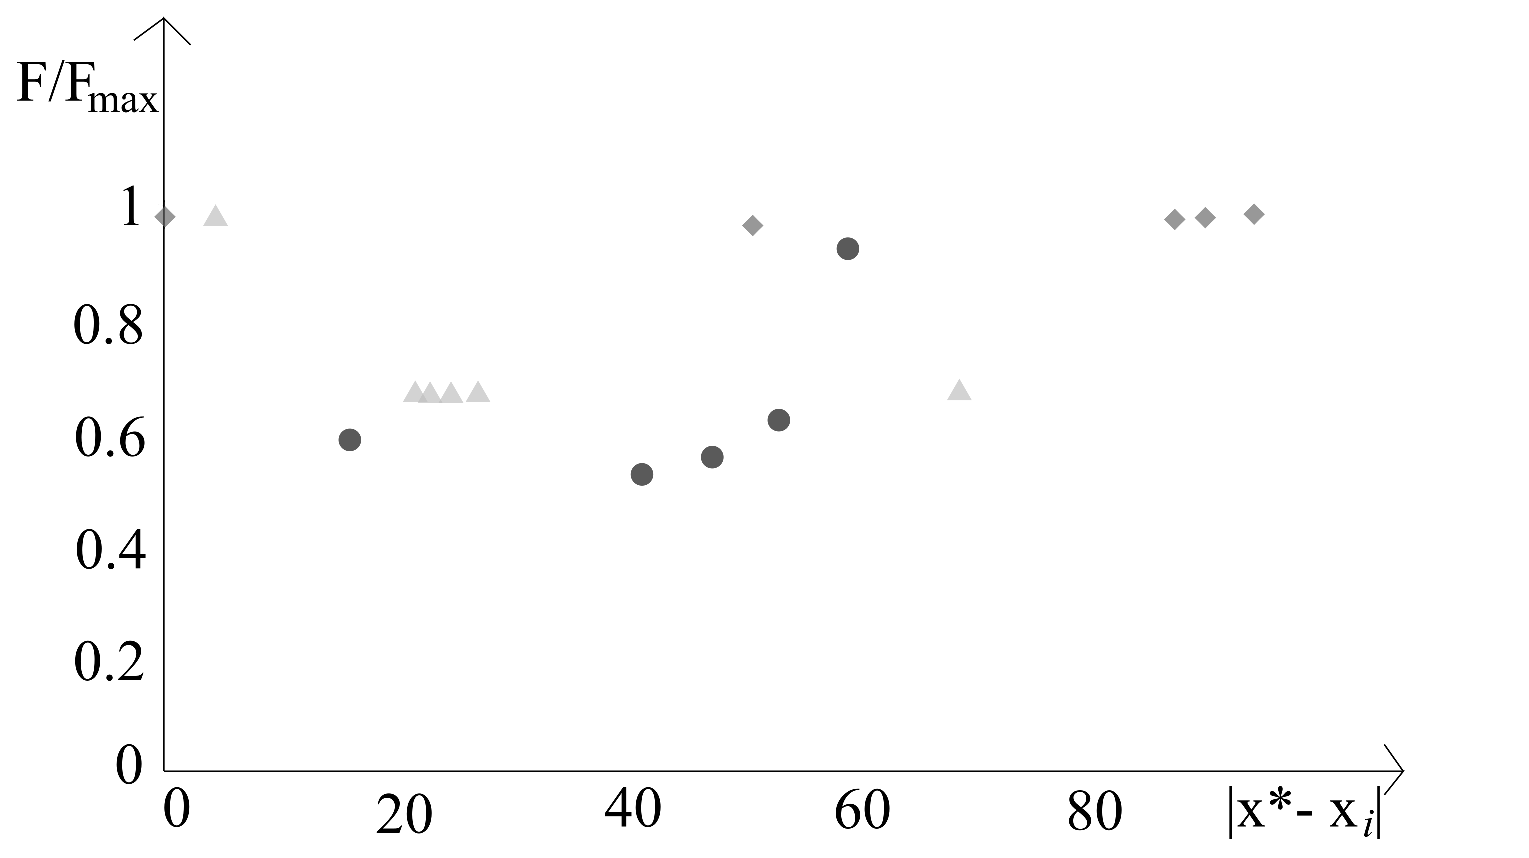
\includegraphics[width=0.9\linewidth]{fit_dist.eps}  \\ а) }
    \end{minipage}
    \begin{minipage}[h]{0.8\linewidth}
            \center{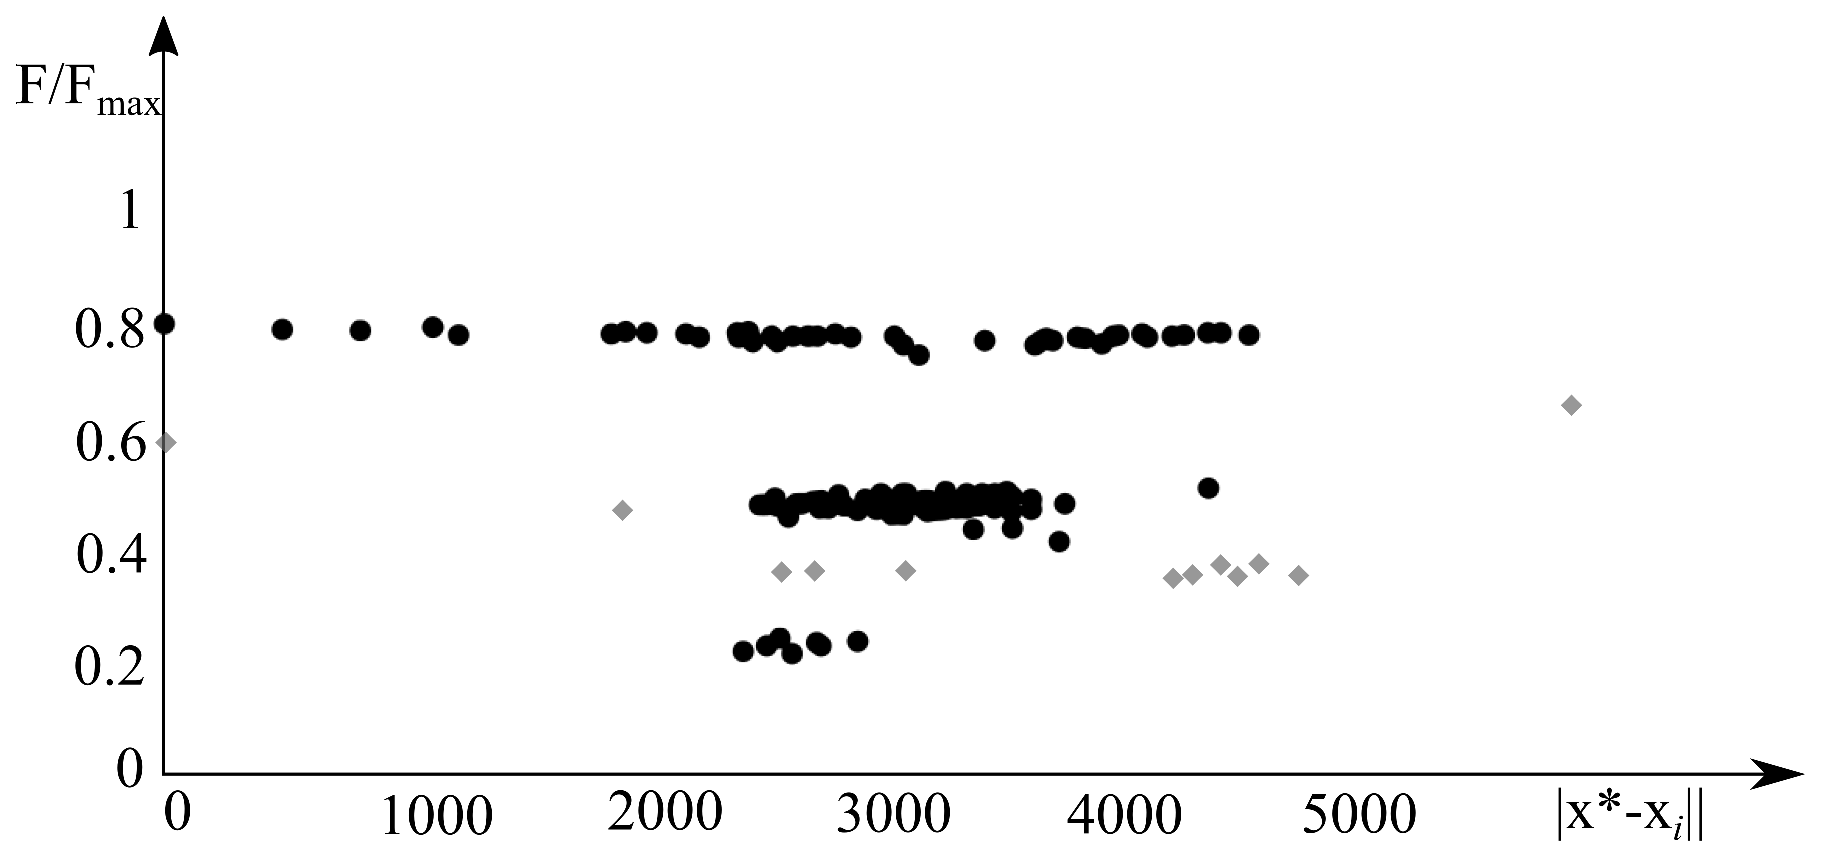
\includegraphics[width=0.9\linewidth]{fit_dist_2x2.eps}  \\ б) }
    \end{minipage}
    \vspace{0.7em}
    \caption{Структура множества найденных решений для задач ШВИ, ШВД, СВД (а) и СВД' (б)}
    \label{ris:fit_dist}
\end{figure}

Для оценки общего числа локальных оптимумов использовался метод переписи Шнабеля. Данный метод имеет применение в экологии и заключается в
выводе статистических оценок численности популяции на основе числа особей, помеченных в результате эксперимента, из популяции с неизменным
составом, где каждая особь имеет константную вероятность отлова. В~\cite{eremeev:confidence} предлагается адаптация такого метода для оценки числа локальных оптимумов. В таблице~\ref{tab:structure} приводится статистика по числу различных точек остановки (в пределах заданной точности) процедуры мультистарта в течение 1000~с. процессорного времени. Для каждого решения была применена процедура линеаризации задачи и проверки необходимых условий локальной оптимальности, описанная в разделе~(\ref{sec:loc}). Приемлемыми считались отличия целевой функции линеаризованной задачи от значения целевой функции, найденного градиентным методом менее чем на 1\%. Здесь {$M$} - число выполненных запусков за отведенное время, $M_{ne}$ - число групп решений, отличающихся не более чем на 10\% по каждой из координат, {$M_{f}$} - число групп значений целевой функции у таких неэквивалентных решений (с точностью до 10\%, приведенных в таблице~\ref{tab:results}). {$M_{y\approx0}$} - число групп решений, для которых были выполнены необходимые условия локальной оптимальности. $\mathcal{B}$ и $\mathcal{L}$ - оценка нижней границы и оценка максимального правдоподобия числа локальных оптимумов, рассчитанные по методу переписи Шнабеля. Доверительная вероятность для данного метода была выбрана равной 95\%. Оценки для числа решений с различными значениями целевой функции обозначены $\mathcal{B}_{M_f}$ и $\mathcal{L}_{M_f}$. Оценки для числа решений, для которых были выполнены необходимые условия локальной оптимальности, обозначены $\mathcal{B}_{M_{y\approx0}}$ и $\mathcal{L}_{M_{y\approx0}}$.
В случае СВД и СВД' конфигурации 5x5 в течение 1000~с градиентный метод не достиг решения, удовлетворяющего условию остановки, поэтому
данный результат не включен в таблицу~\ref{tab:structure}.

Как видно из таблицы, во всех экспериментах в некоторых запусках были найдены неразличимые с практической точки зрения решения. Для квадратных решеток ШВИ и ШВД было найдено по одному такому решению. Решетки кольцевой структуры и СВД'~2x2 имеют значительное разнообразие как по найденным векторам решений, так и по значениям целевой функции. Относительно решений, для которых были выполнены необходимые условия локальной оптимальности, можно сказать, что с большой вероятностью для задачи СВД'~2x2, были найдены далеко не все возможные решения. О решетке СВД'~3x3 известно, что градиентный подъем был остановлен в точке, не лежащей в окрестности решения, предоставляемого решателем BARON.

На рис.~\ref{ris:fit_dist} приведены диаграммы локальных оптимумов, где по оси ординат отложены значения целевой функции, а по оси
абсцисс - расстояние до лучшего известного решения. В случае а) точками обозначены результаты для кольцевых решеток, состоящих из 8 излучателей, ромбами - для кольцевых решеток, состоящих из 16 излучателей, пятиугольниками - для СВД~3x3. В случае б) точками обозначены результаты для СВД'~2x2, ромбами - для СВД'~3x3. Диаграмма показывает, что значения, соответствующие одному и тому же значению целевой функции, могут находиться достаточно далеко друг от друга, что позволяет сделать предположение о наличии неучтенных симметрий задачи (о множестве линейных симметрий задачи см. в~\cite{yurkov:symmetry}).

\section{Проверка необходимых условий локальной оптимальности} \label{sec:loc}

Как уже было отмечено, нахождение даже локального оптимума в случае решения задачи невыпуклого квадратичного программирования, вообще говоря, является NP-трудным. В связи с этим, применительно к градиентному подъему, можно ожидать ситуаций, в которых при поиске локального оптимума потребуется чрезмерно большое число итераций или произойдет преждевременная остановка вдалеке от локального оптимума. Из этого следует, что имеет смысл предусмотреть процедуру, позволяющую определить случаи, когда полученное решение не является локальным оптимумом. Для этого была применена процедура проверки необходимых условий локальной оптимальности~\cite{murty:np}. Суть данной проверки в том, что мы линеаризуем задачу вблизи точки остановки градиентного алгоритма. Для этого в окрестности решения $\textbf{x}_0$ вводим малое приращение $\textbf{у}$. При этом, каждая квадратичная форма, представленная симметричной матрицей $\textbf{M}$, преобразуется следующим образом:
$$\textbf{x}^T\textbf{M}\textbf{x} = \textbf{x}_0^T\textbf{M}\textbf{x}_0 +
\textbf{x}_0^T\textbf{M}\textbf{y} + \textbf{y}^T\textbf{M}\textbf{x}_0 +
\textbf{y}^T\textbf{M}\textbf{y}.$$ Учитывая симметричность каждой квадратичной формы и пренебрегая квадратичными по $\textbf{y}$ слагаемыми, получаем для задачи~(\ref{eq:task3}):


\begin{equation}
    \begin{cases}
       \textbf{x}_0^T\textbf{G}\textbf{x}_0 + 2\textbf{x}_0^T\textbf{G}\textbf{y} \rightarrow \max,\\
       0 \leq \textbf{x}_0^T\textbf{H}^{(1)}\textbf{x}_0 + 2\textbf{x}_0^T\textbf{H}^{(1)}\textbf{y} \leq 1,\\
       ...\\
       0 \leq \textbf{x}_0^T\textbf{H}^{(n)}\textbf{x}_0 + 2\textbf{x}_0^T\textbf{H}^{(n)}\textbf{y} \leq 1,\\
      \textbf{y} \in \mathbb{R}^{2N}.\\
     \end{cases}
     \label{eq:task5}
\end{equation}

В случае локальной оптимальности решения $\textbf{x}_0$ модуль $|\textbf{y}^T\textbf{G}\textbf{y}|$ должен быть равен нулю.

Следует отметить, что решение задачи~(\ref{eq:task5}) не подтверждает локальную оптимальность, а лишь предоставляет вспомогательную процедуру, благодаря которой из всего множества решений, найденных в результате многократного запуска из случайно сгенерированной точки
градиентного подъема, можно исключить решения, заведомо не являющиеся локальными оптимумами. Такие решения могут быть получены в результате преждевременного завершения работы градиентного метода по точности, если значения целевой функции слабо меняются за итерацию алгоритма или текущее решение оказалось в стационарной точке, не являющейся локальным оптимумом (последнее случается крайне редко).

\section{Экспериментальная проверка устойчивости решений}
\begin{figure}[h]
    \centering
    \center{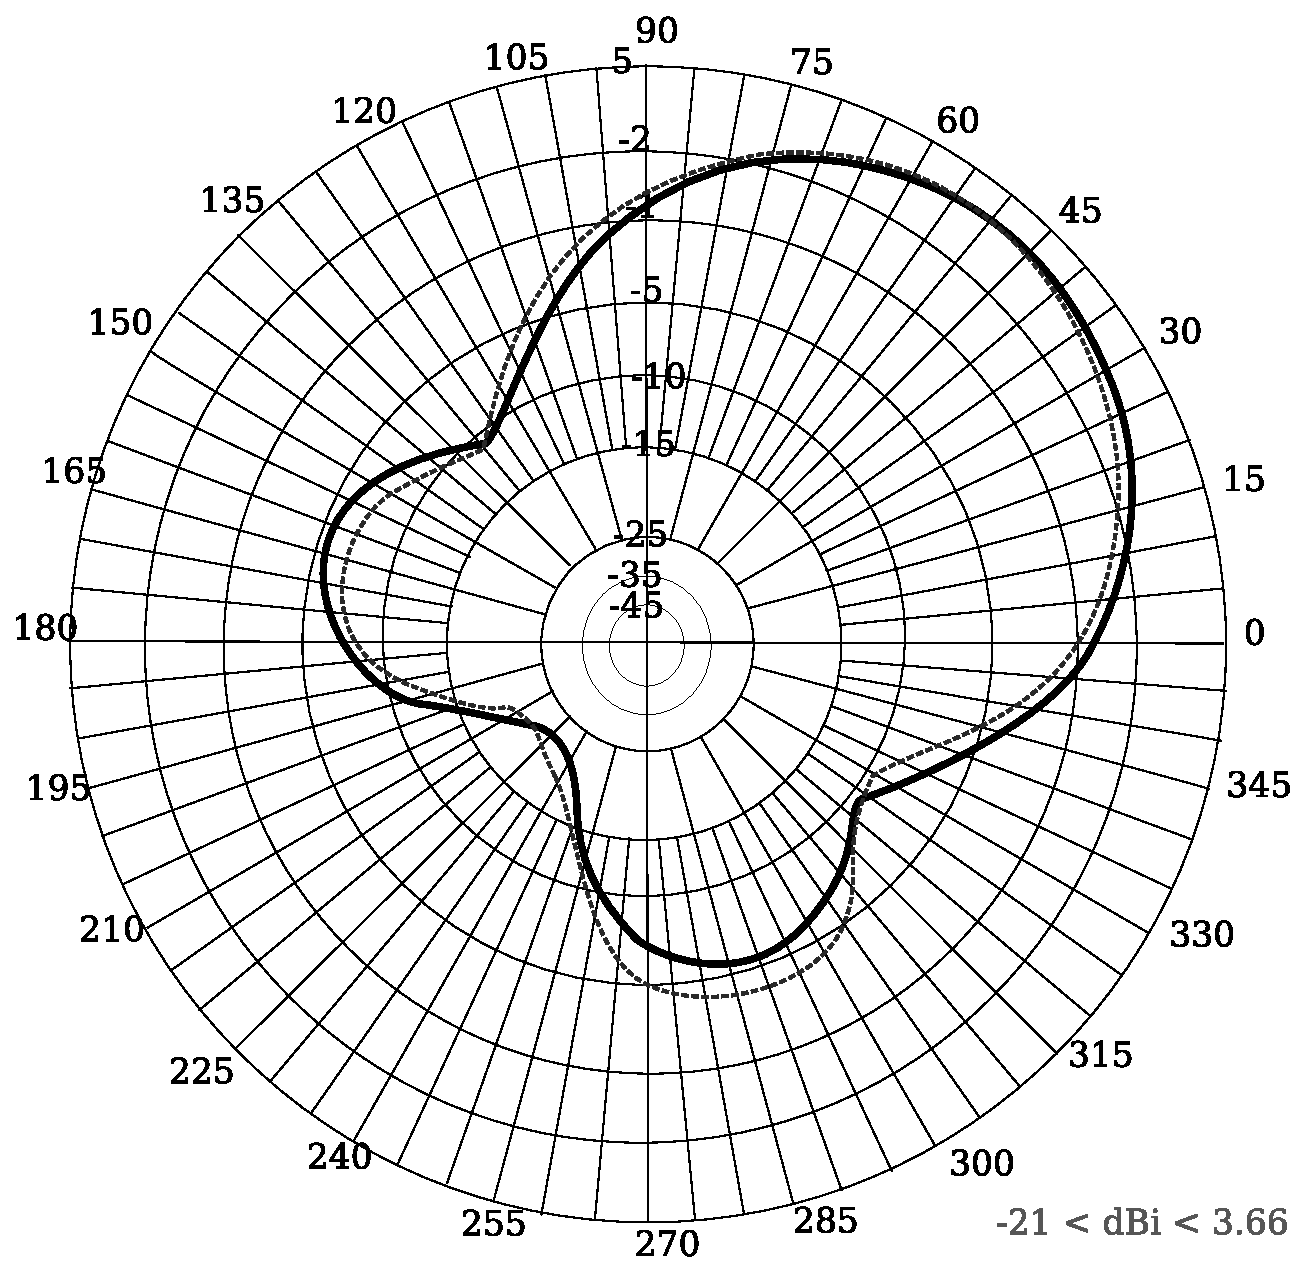
\includegraphics[width=0.5\linewidth]{stability.eps} }
    \vspace{0.7em}
    \caption{Диаграммы направленности для ШВИ~2x2 при оптимизации в направлении 70:45 (сплошная линия) и 70:50 (пунктир)}
    \label{ris:bve_comp}
\end{figure}
При анализе структуры локальных оптимумов может возникнуть вопрос об устойчивости решения по аргументу. В данной работе было проведено исследование изменения значения целевой функции при изменении оптимизируемого направления на малый угол. В рассмотрение принималось также изменение значения целевой функции при подстановки в исходную задачу решения, найденного для нового направления (для удобства вывода результата такая подстановка обозначена за P1), и наоборот - при подстановке в задачу для измененного направления решения, полученного для исходного направления (обозначается P2). Исследование проводилось на квадратных решетках, состоящих из 4-х и 9-и излучателей. Азимутальный и полярный угол менялись на $5^{\circ}$. Результаты приведены в таблице~\ref{tab:stability}
\begin{table}[!h]
\centering
\begin{tabular}{|c|c|c|c|c|c|c|c|}
    \hline
    \textbf{ФАР} & \textbf{Подстановка} & \textbf{70:45} & \textbf{75:45} & \textbf{65:45} & \textbf{70:50} & \textbf{75:40} & \textbf{65:50}\\
    \hline
    \multirow{3}{*}{ШВИ 2x2} & - & \multirow{3}{*}{138} & 125 & 138 & 137 & 137 & 125\\
    & P1 &  & 138 & 138 & 137 & 137 & 137\\
    & P2 &  & 125 & 138 & 136 & 136 & 123\\
    \hline
    \multirow{3}{*}{ШВИ 3x3} & - & \multirow{3}{*}{575} & 532 & 565 & 574 & 533 & 564\\
    & P1 &  & 574 & 572 & 560 & 558 & 557\\
    & P2 &  & 530 & 562 & 559 & 517 & 546\\
    \hline
    \multirow{3}{*}{ШВД 2x2} & - & \multirow{3}{*}{459} & 518 & 454 & 454 & 512 & 389\\
    & P1 &  & 458 & 459 & 457 & 456 & 389\\
    & P2 &  & 518 & 392 & 452 & 510 & 386\\
    \hline
    \multirow{3}{*}{ШВД 3x3} & - & \multirow{3}{*}{1501} & 1817 & 872 & 1015 & 1196 & 1198\\
    & P1 &  & 1506 & 1047 & 1000 & 1004 & 1448\\
    & P2 &  & 1774 & 1203 & 1450 & 1713 & 1162\\
    \hline
    \multirow{3}{*}{СВД 2x2} & - & \multirow{3}{*}{369} & 417 & 315 & 365 & 412 & 312\\
    & P1 &  & 368 & 369 & 367 & 366 & 367\\
    & P2 &  & 417 & 315 & 363 & 410 & 310\\
    \hline
    \multirow{3}{*}{СВД 3x3} & - & \multirow{3}{*}{1484} & 1789 & 1176 & 1459 & 1162 & 1753\\
    & P1 &  & 1475 & 1472 & 1446 & 1428 & 1444\\
    & P2 &  & 1782 & 1164 & 1427 & 1120 & 1713\\
    \hline
\end{tabular}
    \caption{Значения целевой функции при изменении оптимизируемого направления на малый угол.}
    \label{tab:stability}
\end{table}

Результаты исследования показывают, что изменение направления оптимизации на малый угол соответствуют повороту исходной диаграммы направленности на этот угол.

\section{Исследование симметрий задачи}

Для полноты изложения в разделах \ref{sec:sym_common} и \ref{sec:sym_cont} приводятся элементы теории из~\cite{yurkov:symmetry}.
\subsection{Общие положения}
\label{sec:sym_common}
Решение и анализ задач математического программирования может быть упрощен при наличии симметрий этих задач, соответствующих некоторым линейным преобразованиям. В частности, знание таких симметрий может быть использовано для уменьшения размерности задачи, ограничения пространства поиска или получения нового локального оптимума из имеющегося. Эти методы применимы в
случае непрерывной области решений~\cite{CHL13,GATERMANN200495,KWM19}, а также в целочисленном программировании~\cite{BHJ13,C99,Kolokolov2012,Margot2010,Simanchev96} и смешанном целочисленном программировании~\cite{L12,PR19}.
Хотя, в большинстве случаев, применение симметрий направлено на ускорение работы алгоритмов точной оптимизации, в некоторых случаях знание симметрий может оказаться полезным и при разработке и анализе эвристик, в частности, эволюционных алгоритмов~\cite{Doerr21,Adam2004}.

В настоящей работе исследуется случай непрерывной области решений. В то время как предыдущие исследования симметрии в математическом программировании обычно имели дело с перестановками координат пространства решений~\cite{Kolokolov2012,KWM19,L12}, в данной рассматривается большая группа обратимых линейных преобразований. Мы изучаем частный случай задачи квадратичного программирования с квадратичными ограничениями в~${\mathbb R}^N$: целевая функция и ограничения задаются квадратичными формами $\textbf{G}, $ и $\textbf{H}_1,\dots,\textbf{H}_n,$ в виде~(\ref{eq:task3}). Следует еще раз отметить, что все матрицы $\textbf{G}, $ и $\textbf{H}_1,\dots,\textbf{H}_n,$ симметричны и $\textbf{H}_\Sigma = \sum_{i=1}^{n}\textbf{H}_i$ положительно определена.
Без потери общности будем считать, что все ограничение заданы неравенствами~$\le$.
Известная задача о максимальном разрезе (которая является NP-трудной) также может быть сведена к задаче квадратичного программирования с такими свойствами~\cite{Shor1998}.

Под симметрией задачи~(\ref{eq:task3}) подразумевается набор линейных преобразований
%of the column space
\begin{equation}
\label{eq:Lin}
\textbf{x} \to \textbf{y}=\textbf{Px} \, ,
\end{equation}
%

определенный невырожденной матрицей $\textbf{P}$, такой что задача~(\ref{eq:task3}), выраженная в терминах преобразованного пространства
(т.е, через вектор-столбец $\textbf{y} $), совпадает с исходной задачей. Таким образом, в терминах вектора $\textbf{y}$ задача~(\ref{eq:task3}) формулируется в той же форме.
%
\begin{equation}
\label{eq:Tinit}
\left\{
\begin{array}{l}
\displaystyle
\textbf{y}^T \textbf{G y} \to {\max} \, , \\
\displaystyle
\textbf{y}^T\textbf{H}_1\textbf{y} \le  1 \, , \\
\displaystyle
\dots \\
\textbf{y}^T\textbf{H}_n\textbf{y} \le 1 \, ,
\end{array}
\right.
\end{equation}
%
\textit{с той же самой} матрицей $\textbf{G} $ и тем же набором матриц $\{\textbf{H}_i: i=1,\dots,n\}$. Подчеркнем, что, поскольку перестановка ограничений не меняет задачи, матрицы $\textbf{H}_i$ также могут быть пронумерованы произвольно.

Преобразования, заданные матрицами $\textbf{P}$, составляют группу обратимых линейных симметрий, которую мы обозначаем через~$\mathcal G$. Цель статьи -- проанализировать группу~$\mathcal G$ и предложить методы нахождения этой группы {в некоторых частных случаях}. Частичное решение этой проблемы, т.е. нахождение хотя бы подгруппы в~$\mathcal G$, также может иметь смысл для практических целей, если полученные симметрии позволяют упростить данную оптимизационную задачу.

В некоторых случаях также может потребоваться найти группу симметрии только набора ограничений. Обозначим эту группу через~$\mathcal G'$.
Очевидно, это мало чем отличается от поиска группы симметрии~$\mathcal G$ задачи; нужно просто исключить из рассмотрения матрицу $\textbf{G}$ (формально можно считать, что $\textbf{G}$ в этом случае нулевая матрица). Обратите внимание, что $\mathcal G$ является подгруппой в $\mathcal G'$.
{
Кроме того, набор симметрий ограничений тесно связан, но не обязательно идентичен набору тех обратимых линейных преобразований, которые биективно отображают область допустимости задачи ${\mathcal D}:=\{\textbf{x}\in {\mathbb R}^N \ : \ \textbf{x}^T B_i \textbf{x} \le 1, \ i=1,\dots,M\}$ на себя. Группа симметрии множества ограничений~$\mathcal{G}'$ может быть подгруппой в группе симметрии обратимых линейных преобразований области~${\mathcal D}$. Это происходит, например, если имеется несколько ``неактивных'' ограничений, каждое из которых определяет такое множество точек, внутри которого содержится ${\mathcal D}$. Тогда требование, чтобы набор матриц этих ``неактивных'' ограничений оставался в~(\ref{eq:Tinit}), является избыточным относительно группы преобразований области~${\mathcal D}$. В качестве простого примера рассмотрим случай $n=N+1,$ $\textbf{G}={diag}(1,\dots,1), \ \textbf{H}_1={diag}(1,0,0,\dots ,0), \dots, \textbf{H}_N={diag}(0,0,\dots,0,1), \textbf{H}_{N+1}={diag}(1,\dots,1).$ Ясно, что здесь $\textbf{H}_1,\dots,\textbf{H}_N$ определяют ``неактивные'' ограничения, группа обратимых линейных преобразований области~${\mathcal{D}}$ состоит из всех ортогональных преобразований в~${\mathbb R}^N $, а группа $\mathcal G$ — конечная группа линейных симметрий $N$-мерного гиперкуба.
}

Авторы~\cite{GATERMANN200495} объединяют последнее определение симметрии области допустимости с инвариантностью целевой функции для изучения геометрических, алгебраических и вычислительных свойств, подразумеваемых такими (дискретными) симметриями в полуопределенных программах. В этом случае с помощью симметрий получается эквивалентная задача выпуклой оптимизации с меньшим числом переменных и тем же оптимальным решением.

В~\cite{L12} группа формулировок задачи математической оптимизации была определена как множество перестановок индексов переменных, для которых целевая функция и ограничения остаются неизменными. Ясно, что эта группа является подгруппой в $\mathcal{G}$. На основе подхода из~\cite{L12}, в~\cite{KWM19} был разработан алгоритм обнаружения симметрии для задач квадратичного программирования. Этот алгоритм можно использовать для нахождения группы формулировок в нашем случае, однако мы стремимся найти всю группу~$\mathcal{G}$, если это возможно.

Обозначим множество матриц $\textbf{H}_1,\dots,\textbf{H}_n$ через ${\mathcal{H}}$.

\begin{definition} \label{def:invariance}
${\mathcal H}$ называется {\em конгруэнтным инвариантом} (или просто инвариантом, для краткости) относительно преобразования
%
\begin{equation}
\label{transform}
\textbf{H} \to \textbf{P}^T \textbf{H P} \,
\end{equation}
%
с невырожденной матрицей $P$, если $\{P^T \textbf{H} P \ : \ \textbf{H} \in {\mathcal H}\}= \{\mathcal H\}$.
\end{definition}

Множество всех матриц $P$, для которых множество ${\mathcal{Р}}$ является инвариантом, образует группу. Здесь эта группа называется {\em группа симметрий множества матриц}~${\mathcal{Р}}$ и обозначается~${\mathcal{G}}_{\mathcal{H}}$. Ясно, что относительно преобразования $\textbf{H} \to \textbf{P}^T \textbf{H P},$ некоторые матрицы из $\mathcal{H}$ могут сводится к другим, однако, не все возможные комбинации могут быть получены этим способом.

Заметим, что одним из инвариантов преобразования~(\ref{transform}) является {\em инерция} матрицы~$\textbf{H}$,
определяется как упорядоченная тройка: (i)~количество положительных собственных значений~$\textbf{H}$, (ii)~количество отрицательных собственных значений~$\textbf{H}$ и (iii)~количество нулевых собственных значений~$\textbf{H}$ (см., например,~\cite{horn:matrix}, \S~4.5). Таким образом, можно переставлять только матрицы с одинаковой инерцией, а все множество ${\mathcal{H}}$ разбивается на классы эквивалентности матриц с одинаковой инерцией. Это отражено в следующем определении.
\begin{definition}
{\em I-класс} является максимальным по включению подмножеством ${\mathcal{H}}$, состоящим из матриц с равной инерцией.
\end{definition}

Предполагается, что все I-классы ${\mathcal{H}}$ пронумерованы целым числом~$k$ и обозначены~${\mathcal{H}}^I_k$. Обозначим
%
\begin{equation}
{\mathcal{H}} = \bigcup_k {\mathcal{H}}^I_k \, .
\end{equation}
%

Кроме того, сумма \textit{всех} матриц, принадлежащих некоторому I-классу, является инвариантом любого преобразования~(\ref{transform}) из ${\mathcal{G}}_{\mathcal{H}} $

Заметим, что это не все инвариантные суммы, поскольку любая сумма нескольких классов инерции также является инвариантом. Таким образом, по множеству $ {\mathcal{H}} $ можно явно построить набор матриц, инвариантных относительно всех преобразований~(\ref {transform}), перебирая все комбинации I-классов и суммируя их элементы.

\begin{definition}
Любая матрица, являющаяся суммой всех матриц, принадлежащих одному или нескольким I-классам, называется {\em матрицей инвариантности I-типа.}
\end{definition}

%Могут существовать и другие матрицы инвариантности, однако способы их нахождения, и проверка их существования в настоящще время не выяснены.

В~\cite{yurkov:symmetry} показано, что можно упростить анализ группы $\mathcal{G}_{\mathcal{B}}$, если хотя бы одна из матриц инвариантности I-типа положительно определена, так как в этом случае мы сможем использовать известные факты о группе ортогональных преобразований~$O(N)$ (см., например,~\cite{Zhelobenko}).

Можно сказать, что

\textbf{Условие I} {\em выполняется, если по меньшей мере одна инвариантная матрица $H^I$ I-типа положительно определена.}

Следует обратить внимание, что симметричная матрица~$\textbf{H}$ может быть представлена как конгруэнтное преобразование диагональной матрицы:
%
\begin{equation}
\label{eq:BSSTDS}
\textbf{H}=\textbf{S}^T\textbf{DS} \, ,
\end{equation}
%
где $\textbf{D}$ -- диагональная матрица, которая может иметь только ``0'', ``1'', или ``-1'' на ее главной диагонали. Матрица $\textbf{S}$ Может быть получена конструктивно, например, конечным методом Лагранжа~(\cite{Lancaster},~Г.~5).

В тех случаях, когда $\textbf{H}$ положительно определена, матрица~$\textbf{D}$ будет являться единичной матрицей и может быть опущена в~(\ref{eq:BSSTDS}).

\begin{proposition} \label{prop:orthogonal} Если условие~I выполняется, тогда группа $ {\mathcal{G}}_{\mathcal{H}} $ является изоморфизмом некоторой подгруппы группы ортогональных преобразований, и этот изоморфизм определяется отображением
\begin{equation}
\label{eq:Qdef_map}
\textbf{P} \to \textbf{SPS}^{-1},
\end{equation}
Где матрица $S$ такова, что $\textbf{H}^I=\textbf{S}^T \textbf{S}.$
\end{proposition}

\begin{proof}
Если матрица $\textbf{H}^I$ положительно определена, тогда условие инвариантности~(\ref{transform}) для $\textbf{H}^I$ обращается в уравнение
%
\begin{equation}
%\label{}
\textbf{P}^T \textbf{S}^T\textbf{SP} = \textbf{S}^T\textbf{S} \,
\end{equation}
%
или
%
\begin{equation}
\label{eqn:unit_matr}
(\textbf{SP}^{-1})^T  (\textbf{SPS}^{-1}) =  E \, ,
\end{equation}
%
где $E$ -- единичная матрица. Это значит, что матрица
%
\begin{equation}
\label{eq:Qdef}
\textbf{Q}:=\textbf{SPS}^{-1}
\end{equation}
%This means that the matrix $Q = STS^{- 1} $, generally speaking, belongs to the pseudo-orthogonal group~\cite{Zhelobenko}.
является группой ортогональных преобразований в~$O(N)$ %\qed
\end{proof}

{
Инвариантность задачи~(\ref{eq:task3}) относительно преобразования~$\textbf{P}$ подразумевает, что
%
\begin{equation}
\label{eq:geninvar}
\textbf{P}^T\textbf{GP}=\textbf{G} \,  , \qquad \textbf{P}^T\textbf{H}_i \textbf{P} = \sum_{j=1}^n \textbf{L}_{ij}\textbf{P}_j , \  i=1,\dots,n,
\end{equation}
%
где $ \textbf{L}_{ij} $ элементы матрицы перестановок, т.е. матрица ${\textbf{L}=(\textbf{L}_{ij})}$ имеет одну единицу в каждом столбце и в каждой строке, остальные элементы~$\textbf{L}$ равны нулю.

Утверждение~\ref{prop:orthogonal} может быть применено для анализа симметрий задачи~(\ref{eq:task3}), если известны некоторые матрицы инвариантности I-типа $\textbf{H}^I$ для множества матриц ${\mathcal{H}}=\{\textbf{H}_1,\dots,\textbf{H}_n\},$ подразумевая, что
%
\begin{equation}
\label{eq:invBS}
\textbf{P}^T \textbf{H}^I \textbf{P} = \textbf{H}^I,
\end{equation}
и { $\textbf{H}^I$ } положительна определена.

В задаче оптимизации направленности ФАР матрица~$\textbf{H}_{\Sigma}:=\sum_i \textbf{H}_i$ положительно определена. Если выполняется~(\ref{eq:geninvar}), тогда $\textbf{H}^I=\textbf{H}_{\Sigma}$ является матрицей инвариантности I-типа для множества матриц ${\mathcal{H}}=\{\textbf{H}_1,\dots,\textbf{H}_n\}.$

Естественно, в общем случае, инвариантность матрицы $\textbf{H}^I$ не обязательно подразумевает выполнение~(\ref{eq:geninvar}), но, по крайней мере, можно говорить, что группа~$\mathcal G'$ является подгруппой ${\mathcal G}_{\mathcal{B}}$, которая, в свою очередь, является подгруппой в $O(N)$ по утверждению~\ref{prop:orthogonal}. Следовательно $\mathcal{G}$ также является подгруппой~$O(N)$.


В дальнейшем всегда будем предполагать, что существует положительно определенная инвариантная матрица $\textbf{H}^I$ I-типа для множества матриц ${\mathcal{H}}=\{\textbf{H}_1,\dots,\textbf{H}_n\},$, т.е. Условие~I выполнено, и $\textbf{Q}$ всегда будет обозначать образ~$\textbf{P}$ при изоморфизме~(\ref{eq:Qdef_map}).

Поскольку $\textbf{P}=S^{-1}\textbf{QS}$ по определению~$\textbf{Q}$, применение~(\ref{eq:geninvar}) дает

%
\begin{equation}
\begin{array}{l}
\displaystyle
(\textbf{S}^{-1}\textbf{QS})^T\textbf{G}(S^{-1}\textbf{QS})=\textbf{G} \,  , \\ \\
\displaystyle
(\textbf{S}^{-1}\textbf{QS})^T\textbf{H}_i (\textbf{S}^{-1}\textbf{QS})= \sum_{j=1}^n \textbf{L}_{ij}\textbf{H}_j \, , \ i=1,\dots,n,
\end{array}
\end{equation}
%

и, после простого преобразования, получается
%
\begin{equation}
\label{eq:invarwithQ}
\textbf{Q}^T \tilde{\textbf{G}} \textbf{Q}=\tilde{\textbf{G}} \,  , \ \ \ \
\textbf{Q}^T \tilde{\textbf{H}_i} \textbf{Q}= \sum_{i=1}^N \textbf{L}_{ij}\tilde{\textbf{H}_j} \, , \ i=1,\dots,n,
\end{equation}
%
где
%
\begin{equation}
\tilde{\textbf{G}}=\left(\textbf{S}^{-1}\right)^T \textbf{G} \textbf{S}^{-1} \, , \qquad
\tilde{\textbf{H}_i}=\left(\textbf{S}^{-1}\right)^T \textbf{H}_i \textbf{S}^{-1} \, , \ i=1,\dots,n.
\end{equation}
%
Таким образом, используя изоморфизм (\ref{eq:Qdef}), мы можем заменить уравнения (\ref{eq:geninvar}) аналогичными уравнениями (\ref{eq:invarwithQ}), но с заменой матриц
\begin{equation}
\label{eq:totilde}
\textbf{G} \to \tilde{\textbf{G}} \, , \qquad \textbf{H}_i \to \tilde{\textbf{H}_i}\, , \ i=1,\dots,n.
\end{equation}
%
и заменив $\textbf{P}$ ортогональной матрицей~$\textbf{Q}$. Эти уравнения значительно проще, так как в этом случае условие~(\ref{eq:invarwithQ}) можно сформулировать линейно в~$\textbf{Q}$:
%
\begin{equation}
\label{eq:comutatinvarwithQ}
\tilde{\textbf{G}} Q=Q\tilde{\textbf{G}} \,  , \ \ \ \
\tilde{\textbf{H}_i} Q= Q\sum_{j=1}^n \textbf{L}_{ij}\tilde{\textbf{H}_j} \, , \  i=1,\dots,n.
\end{equation}
%
Если найти все подходящие ортогональные отображения $\textbf{Q}$, то будет легко восстановить соответствующие матрицы~$\textbf{P}$. В дальнейшем группу таких подходящих матриц~$\textbf{Q}$ мы также будем обозначать через~$\mathcal{G}$, поскольку матрицы~$\textbf{P}$ и $\textbf{Q}$ просто дают разные {точные} представления одной и той же абстрактной группы.

Известно, что ортогональная группа $O(N)$ состоит из двух компонент связности, для одной из которых определитель матрицы равен~1, для другой равен~-1 (см., например,~\cite{Zhelobenko}). Первая компонента — это подгруппа в $O(N)$, обозначаемая $SO(N)$ и также называемая {\em группой вращений} из-за того, что в размерностях 2 и 3 ее элементами являются обычные вращения вокруг точки или линии соответственно. Вторая компонента не образует подгруппу в $O(N)$, так как не содержит единичного элемента. Матрицы из второго компонента могут быть представлены, например, в виде: $ {diag} \{- 1,1 \dots 1 \} \textbf{Q} $, где $ \textbf{Q} \in SO(N) $, поэтому между этими компонентами имеется взаимно однозначное соответствие (которое не является изоморфизмом в теоретико-групповом смысле, так как не сохраняет групповые операции). Искомые матрицы $\textbf{Q}$ могут принадлежать как первой компоненте, так и второй.

Из стандартных фактов теории топологических групп (см., например,~\cite{Zhelobenko},~Г.~1) вытекают следующие свойства группы симметрии~$\mathcal{G},$, наделенной стандартной топологией ${\mathbb R} ^{N^2},$ применительно к пространству $(N\times N)$-матриц. Как всякая топологическая группа, $\mathcal{G}$ состоит из компонент связности (в топологическом смысле), только одна из которых, далее обозначаемая как~$\mathcal{G}_1$, содержит единичный элемент. Эта~$\mathcal{G}_1$ является подгруппой инвариантности группы~$\mathcal{G}$, см. теорему~1 в~\cite{Zhelobenko} и в дальнейшем называется {\em непрерывной подгруппой симметрий}. Остальные компоненты связности (не являющиеся подгруппами) можно рассматривать как произведения элементов группы вне~$\mathcal G_1$ на элементы группы~$\mathcal G_1$, т.е. смежные классы группы~$\mathcal G_1$. Эти смежные классы можно идентифицировать, указав одного (любого) представителя смежного класса.

\subsection{Нахождение групп непрерывных симметрий}
\label{sec:sym_cont}
Рассмотрим более подробно случай непрерывной подгруппы симметрий~$\mathcal{G}_1$. Нетривиальные перестановки матриц $\tilde{\textbf{H}}_i$, если они все разные, не могут быть результатом преобразований, принадлежащих~$\mathcal{G}_1$, так как невозможно непрерывно двигаться от тождественного преобразования (из чего следует, что матрицы $\tilde{\textbf{H}}_i$ не переставляются) любому преобразованию~$\textbf{Q}$, дающему нетривиальную перестановку матриц $\tilde{\textbf{H}}_i$. Заметим, что любая такая~$\textbf{Q}$ имеет окрестность преобразований, не дающих тривиальной перестановки матриц~$\tilde{\textbf{H}}_i$. Поэтому, условие инвариантности~(\ref{eq:comutatinvarwithQ}) подразумевает коммутативность:
%
\begin{equation}
\label{eq:commutat}
\tilde{\textbf{G}} \textbf{Q} = \textbf{Q} \tilde{\textbf{G}}\, , \qquad \tilde{\textbf{H}}_i \textbf{Q} = \textbf{Q} \tilde{\textbf{H}}_i\, , \ i=1,\dots,n.
\end{equation}
%
Следующее утверждение является "фольклорным" фактом матричного анализа (доказательство можно найти в~\cite{yurkov:symmetry}):

\begin{proposition} \label{prop:skew_exp}
Любая матрица $\textbf{Q} \in SO(N) $ может быть представлена как матричная экспоненциальная функция кососимметричной матрицы. Верно и обратное: экспоненциальная функция любой кососимметричной матрицы является ортогональной матрицей.
\end{proposition}

Итак, с некоторой кососимметричной матрицей~$\textbf{X}$ имеем $\textbf{Q}=e^\textbf{X}$. Набор кососимметрических матриц $\textbf{X}$ составляет алгебру Ли, соответствующую этой группе Ли~\cite{Zhelobenko}. Алгебра Ли, соответствующая $SO(N)$, обычно обозначается $so(N)$. Любая алгебра Ли также является линейным пространством, любой ее элемент может быть выражен с помощью базисных элементов, называемых образующими. Таким образом, любой элемент алгебры Ли можно представить в виде:
%
\begin{equation}
\textbf{X} = \sum_n a_n G_n \, ,
\end{equation}
%
где $ a_n $ являются вещественными числами, $G_n $ являются генераторами. Пространство кососимметричных матриц имеет размерность $N(N-1)/2$, а количество коэффициентов $a_n$ будет равно количеству образующих. В качестве образующих можно выбрать матрицы, у которых над главной диагональю все элементы равны~0, кроме одного элемента, равного~1. Тогда кососимметрия однозначно определяет остальные матричные элементы этих генераторов. Итак, любой элемент $Q$ из $SO(N)$ можно представить в виде:
%
\begin{equation}
\label{eq:sunexp}
\textbf{Q}=e^{\sum_n a_n G_n} \, .
\end{equation}
%

Поскольку искомая непрерывная подгруппа симметрии~$\mathcal{G}_1$ является подгруппой в $SO(N)$, то для нее также справедливо представление~(\ref{eq:sunexp}), но, вообще говоря, параметры $ a_n$ теперь не являются независимыми. Таким образом, поиск этой подгруппы по существу сводится к нахождению ограничений на параметры $a_n$.

Совершенно очевидно, что для выполнения условий коммутативности~(\ref{eq:commutat}) достаточно выполнения следующих условий:
%
\begin{equation}
\label{eq:commutat2}
\left\{
\begin{array}{l}
\displaystyle
\tilde{\textbf{H}}_i \left(\sum\limits_na_nG_n\right) =
\left(\sum\limits_na_nG_n\right) \tilde{\textbf{H}}_i \, , \\ \\
\displaystyle
\tilde{\textbf{G}} \left(\sum\limits_na_nG_n\right) = \left(\sum\limits_na_nG_n\right) \tilde{\textbf{G}} \, .
\end{array}
\right.
\end{equation}
%

Заметим, что согласно~(\ref{eq:commutat2}), если матрица $\textbf{X}$ коммутирует со всеми матрицами $\tilde{\textbf{H}}_i$ и с матрицей $\tilde{\textbf{G}}$, то $\textbf{X}$ лежит в алгебре Ли~$ \mathcal{G}_1$.
Действительно, разлагая показательную функцию в степенной ряд, мы видим, что если матрицы $\tilde{\textbf{G}}$ и $\tilde{\textbf{H}}_i$ коммутируют с аргументом этой функции, то они коммутируют и с самой показательной функцией.

%
Условие~(\ref{eq:commutat2}) не обязательно влечет~(\ref{eq:commutat}), однако непрерывная подгруппа симметрий является связной группой Ли, поэтому она полностью определяется своей алгеброй Ли, который полностью определяется ограничительными соотношениями~(\ref{eq:commutat2}) на его элементах. Таким образом, при поиске непрерывной подгруппы симметрии~(\ref{eq:commutat}) можно заменить на~(\ref{eq:commutat2}).

Уравнения~(\ref{eq:commutat2}) представляют собой систему линейных алгебраических уравнений, определяющих параметры $a_n$. Эта система однородна, поэтому она имеет континуум ненулевых решений или одно тривиальное решение. Тривиальное нулевое решение всегда присутствует и соответствует единичной матрице $\textbf{Q}$. Некоторые из параметров $a_n$ остаются ``свободными'' (это будут параметры искомой подгруппы), а остальные из~$a_n$ могут быть линейно выражены через ``свободные''. Решение этой системы уравнений~(\ref{eq:commutat2}) может быть получено конструктивно методом Гаусса.

Условие инвариантности задачи относительно преобразования~$\textbf{Q}$ превращается в
%
\begin{equation}
\label{eq:subG1}
\textbf{Q}=e^{\sum_n a_n \hat{G}_n} \, ,
\end{equation}
%
где сумма идет по "свободным" параметрам $a_n$, а новые генераторы, обозначаемые через~$\hat{G}_n$, являются линейными комбинациями прежних генераторов~$G_n$. Множество всех $\textbf{Q}$-матриц, удовлетворяющих~(\ref{eq:subG1}), параметризуется конечным набором вещественных параметров $a_n$. Заметим, однако, что этот набор матриц не обязательно изоморфен евклидову пространству, поскольку одному и тому же~$\textbf{Q}$ может соответствовать более одного набора параметров $a_n$.

\subsection{Вычислительный эксперимент}
Вычислительный эксперимент состоит из следующих этапов:
\begin{enumerate}
  \item Обработка. На этом этапе возможная неточность данных нивелируется усреднением симметричных компонент матриц (матрицы $\textbf{G}$ и $\textbf{H}$ должны быть симметричны).
  \item %Normalization of matrices $B_i$.
  Преобразование $ {\textbf{H}}_{\Sigma} = \sum_{i} \textbf{H}_i$ к канонической форме используя метод Лагранжа для вычисления матриц~$\textbf{S}$ и $\textbf{S}^{-1} $.
  \item Применение метода Гаусса к системе линейных уравнений~(\ref{eq:commutat2}) для вычисления генераторов~$\hat{G}_n$.
\end{enumerate}

Следует отметить, что входные данные могут содержать некоторые погрешности, которые приводят к несимметричности матриц $\textbf{G}$ и $\textbf{H}$, что может существенно повлиять на поиск непрерывных групп симметрий. Таким образом, на этапе~1, мы используем известные свойства задачи чтобы нивелировать влияние погрешности.
Также, в методе Гаусса на шаге 3, любые значения принимаются за 0 если их абсолютное значение меньше определенного порогового значения~$\Delta$, который является параметром алгоритма. Причина в том, что последовательное исключение переменных из уравнений, выполняемое методом Лагранжа с представлением вещественных чисел с плавающей запятой, не может гарантировать идеальную точность.
В результате некоторые линейно зависимые строки матрицы не могут быть исключены, что может привести к неверному результату.
%To eliminate this effect, a threshold error is introduced.
Большое значение порога~$\Delta$ может привести к вырожденности задачи, тогда как слишком малое значение~$\Delta$ не позволит выявить линейные зависимости.

В данном эксперименте, $\Delta$ изменялось от $ 10^{-4} $ до $ 10^{-12} $. В данном диапазоне для каждого рассмотренного частного случая задачи, не было получено различий в полученных решениях.

%\subsection{Optimization of the Excitation of Antenna Arrays}

Описанная процедура нахождения непрерывных групп симметрий применяется к примерам, описанным в разделе~\ref{subsec:examples}. Для всех рассмотренных задач было выявлено только наличие фазовой симметрии. Возможно, множественность решений объясняется наличием дискретных симметрий. Выявление дискретных симметрий является объектом дальнейших исследований.

В качестве примера приводятся результаты для ШВИ~2x2.

В результате работы алгоритма было выявлено, что все генераторы могут быть выражены через один новый генератор вида
$$
G = \left(\begin{array}{cccccccc}
        0 & 0 & 0 & 0 & -1 & 0 & 0 & 0\\
        0 & 0 & 0 & 0 & 0 & -1 & 0 & 0\\
        0 & 0 & 0 & 0 & 0 & 0 & -1 & 0\\
        0 & 0 & 0 & 0 & 0 & 0 & 0 & -1\\
        1 & 0 & 0 & 0 & 0 & 0 & 0 & 0\\
        0 & 1 & 0 & 0 & 0 & 0 & 0 & 0\\
        0 & 0 & 1 & 0 & 0 & 0 & 0 & 0\\
        0 & 0 & 0 & 1 & 0 & 0 & 0 & 0
\end{array}\right),
$$
который соответствует фазовой симметрии. Для данного генератора при $a = 1$
$$e^{aG} = \left(\begin{array}{cccccccc}
        0.5403 & 0 & 0 & 0 & -0.8415 & 0 & 0 & 0\\
        0 & 0.5403 & 0 & 0 & 0 & -0.8415 & 0 & 0\\
        0 & 0 & 0.5403 & 0 & 0 & 0 & -0.8415 & 0\\
        0 & 0 & 0 & 0.5403 & 0 & 0 & 0 & -0.8415\\
        0.8415 & 0 & 0 & 0 & 0.5403 & 0 & 0 & 0\\
        0 & 0.8415 & 0 & 0 & 0 & 0.5403 & 0 & 0\\
        0 & 0 & 0.8415 & 0 & 0 & 0 & 0.5403 & 0\\
        0 & 0 & 0 & 0.8415 & 0 & 0 & 0 & 0.5403
\end{array}\right).
$$

Результаты данного раздела были представлены в~\cite{tyu:daor, tyu:motor}. 
\chapter{Исследование возможностей ФАР в разных условиях}\label{sec:radio}

\section{Исследование радиочастотных зависимостей}
 На практике использование высоко симметричных ФАР вызывает особый интерес из следующих соображений: измерение матрицы сопротивлений является тривиальной задачей, в то время как измерение парциальных полей требует большое количество приемников для всех возможных направлений излучения. Использование высокосимметричных ФАР позволяет выполнить расчеты для одного направления и затем легко адаптировать их для дугих симметричных направлений. Другой особенностью, влияющей на результаты моделирования является наличие потерь в земле (см.~\cite{yurkov:groundloss}). Чтобы ослабить этот эффект, антенные системы с противовесами подняты над землей на 2 м.

В данной главе мы изучаем, как изменяется общий коэффициент усиления с ростом радиочастоты и плотности системы противовесов. Общий коэффициент усиления является суммой частичных коэффициентов усиления в  двух ортогональных поляризациях. Плотность системы противовесов определяется числом продольных и поперечных проводов, относящихся к одному и тому же излучателю. Частота изменяется от 5 до 30 МГц. Вычисления производились на решетках ШВИ, состоящих из 8 излучателей. Для расчета матрицы сопротивлений и матрицы излучений использовался пакет моделирования антенных систем NEC2~\cite{bruke:nec2}.

Для проведения вычислительного эксперимента использовался решатель BARON в пакете GAMS, поскольку, в основном он деонстрирует лучшие результаты по сравнению с градиентным подъемом. Результаты оптимизации направленности решетки сравниваются с коэффициентом усиления одиночного излучателя, установленного в центре такой же системы противовесов. Плотность системы противовесов обозначается в формате $long:trans$, где $long$ - число продольных проводов, относящихся к одному излучателю, а $trans$ - поперечных. Высота каждого ШВИ - 15м. В качестве направления оптимизации выбирается $70^{\circ}$ полярного угла и $45^{\circ}$ азимутального угла в сферических координатах.

\begin{figure}
\center{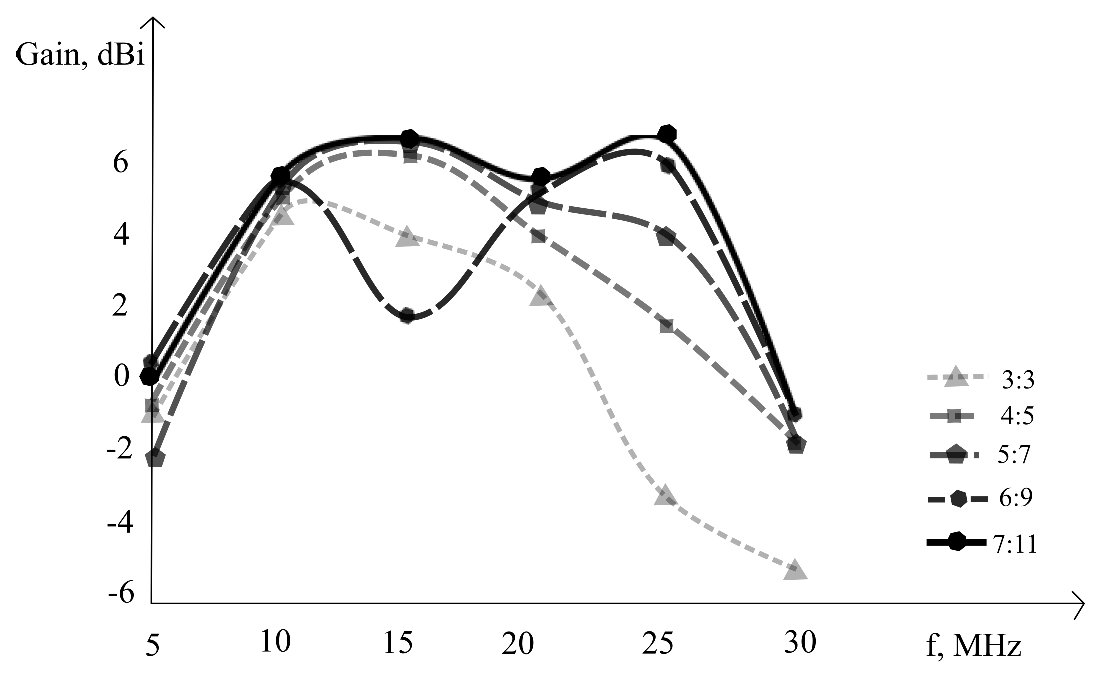
\includegraphics[width=0.8\linewidth]{ring_f__paa_gains.eps}}
\caption{Зависимость от частоты общего коэффициента усиления ФАР при оптимизации в направлении 70:45}
\label{ris:paa_gains}
\end{figure}

На рис.~\ref{ris:paa_gains} показано, как изменяется коэффициент усиления с ростом радиочастоты. Мы можем наблюдать, что при значениях частоты 5 и 30 МГц решетка оптимизируется довольно плохо. Также можно увидеть, что, в основном, увеличение плотности системы противовесов приводит к росту коэффициента усиления. Единственное исключение - решетка с плотностью системы противовесов $6:9$ на частоте 15МГц, где наблюдается неожиданное падение коэффициента усиления. Такое поведение может быть объяснено тем, что BARON не достиг глобалного оптимума.

\begin{figure}
\center{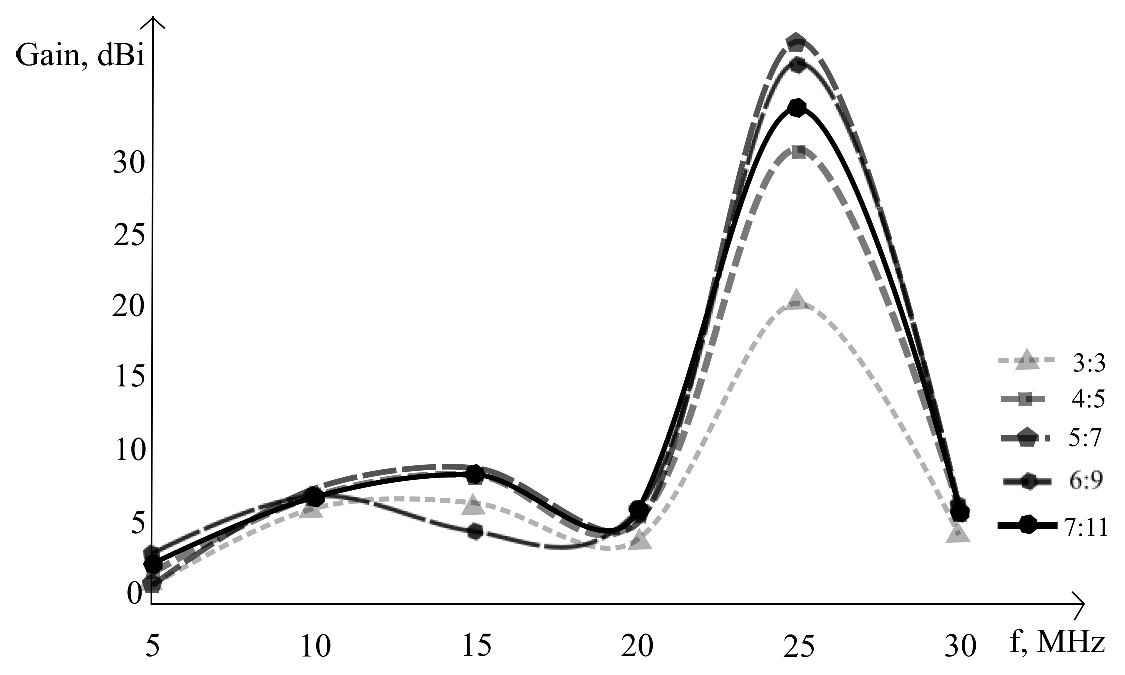
\includegraphics[width=0.8\linewidth]{ring_f_gains.eps}}
\caption{Сравнение коэффициентов усиления ФАР и одиночного излучателя}
\label{ris:all_gains}
\end{figure}

На рис.~\ref{ris:all_gains} показано, как изменяется разница коэффициентов усиления ФАР и одиночного излучателя с ростом частоты. Заметным результатом здесь является то, что на частоте 25МГц усиление ФАР существенно больше усиления одиночного излучателя. Объяснение этого эфффекта будет приведено далее при сравнении диаграмм направленности. При 5МГц усиление ФАР существенно не превосходит усиление одиночного излучателя, однако, уже на 10МГц разница возрастает до 7.53дБ. Даже при 30МГц, где ФАР не оптимизируется хорошо, разница с одиночным излучателем составляет 6.63дБ в лучшем случае и 4.84дБ в худшем.

Далее будут рассмотрены диаграммы направленности ФАР с плотностью противовесов $5:7$ как один из наиболее типичных результатов.

\begin{figure}
\begin{minipage}[h]{0.49\linewidth}
\center{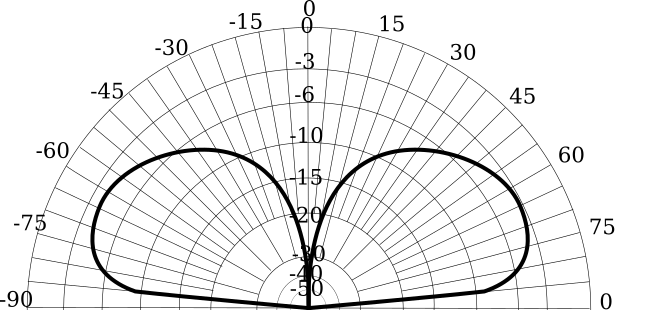
\includegraphics[width=1\linewidth]{r8_1_5_5x7.png} \\ a)}
\end{minipage}
\hfill
\begin{minipage}[h]{0.49\linewidth}
\center{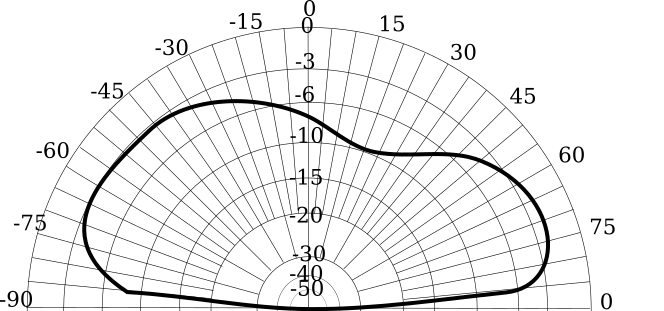
\includegraphics[width=1\linewidth]{r8_5_5x7.png} \\ b)}
\end{minipage}
\caption{Вертикальный план диаграммы направленности одиночного излучателя (a) и ФАР 5:7 (b) при 5МГц}
\label{ris:5MHz}
\end{figure}

При частоте 5МГц (см Рис.~\ref{ris:5MHz}) мы можем наблюдать, что максимум усиления в случае ФАР приходится на $70^{\circ}$ и превосходит соответствующее значение одиночного излучателя на 1.33~дБ. Использование ФАР с плотностью системы противовесов 6:9 позволяет увеличить этот параметр до 3.14~дБ.

\begin{figure}
\begin{minipage}[h]{0.49\linewidth}
\center{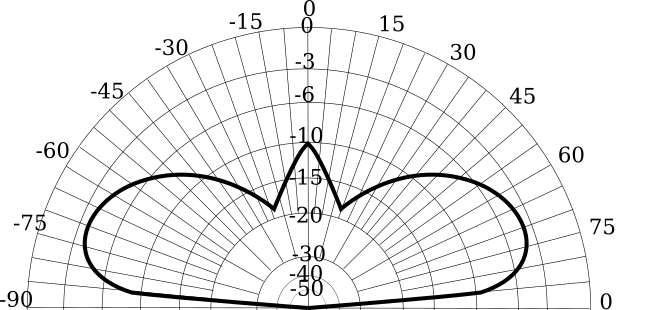
\includegraphics[width=1\linewidth]{r8_1_10_5x7.png} \\ a)}
\end{minipage}
\hfill
\begin{minipage}[h]{0.49\linewidth}
\center{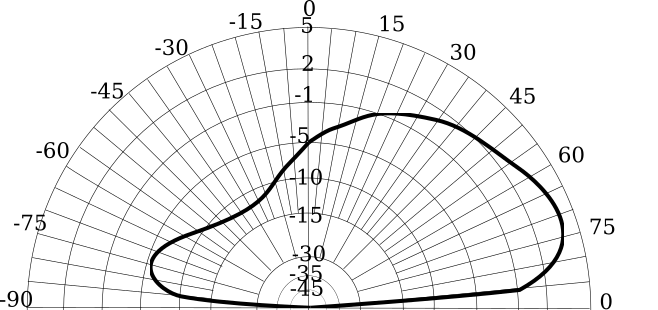
\includegraphics[width=1\linewidth]{r8_10_5x7.png} \\ b)}
\end{minipage}
\caption{Вертикальный план диаграммы направленности одиночного излучателя (a) и ФАР 5:7 (b) при 10МГц}
\label{ris:10MHz}
\end{figure}

Результат оптимизации более заметен при частоте 10МГц~(см~Рис.~\ref{ris:10MHz}): задний лепесток существенно меньше и разница усиления к одиночному излучателю достигает примерно~8~дБ. Похожие результаты наблюдаются при частоте~15МГц.

\begin{figure}
\begin{minipage}[h]{0.49\linewidth}
\center{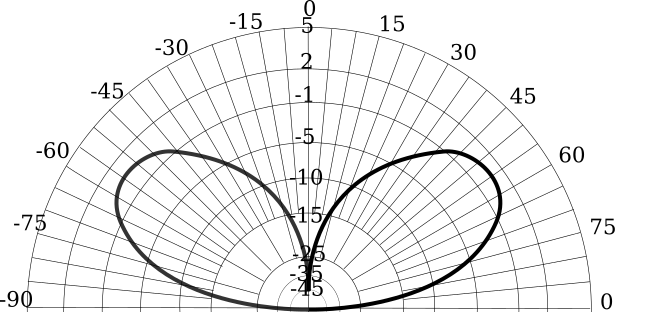
\includegraphics[width=1\linewidth]{r8_1_20_5x7.png} \\ a)}
\end{minipage}
\hfill
\begin{minipage}[h]{0.49\linewidth}
\center{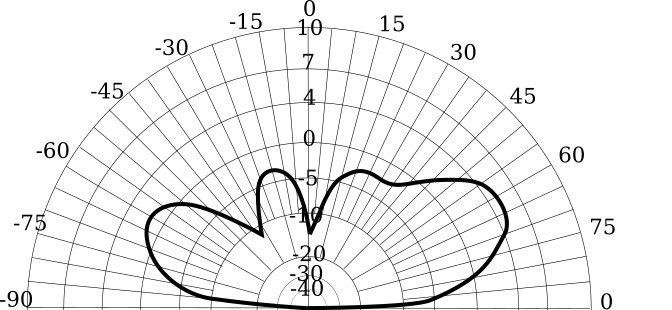
\includegraphics[width=1\linewidth]{r8_20_5x7.png} \\ b)}
\end{minipage}
\caption{Вертикальный план диаграммы направленности одиночного излучателя (a) и ФАР 5:7 (b) при 20МГц}
\label{ris:f20mhs}
\end{figure}

При 20МГц мы можем наблюдать, что как в случае одиночного излучателя, так и в случае ФАР, коэффициент усиления падает по отношению к результату при 15МГц~(см~Рис.~\ref{ris:paa_gains}). Диаграмма направленности изображена на рис.~\ref{ris:f20mhs}.

\begin{figure}
\begin{minipage}[h]{0.49\linewidth}
\center{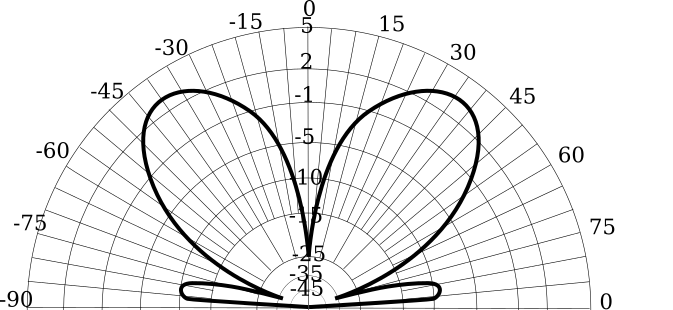
\includegraphics[width=1\linewidth]{r8_1_25_5x7.png} \\ a)}
\end{minipage}
\hfill
\begin{minipage}[h]{0.49\linewidth}
\center{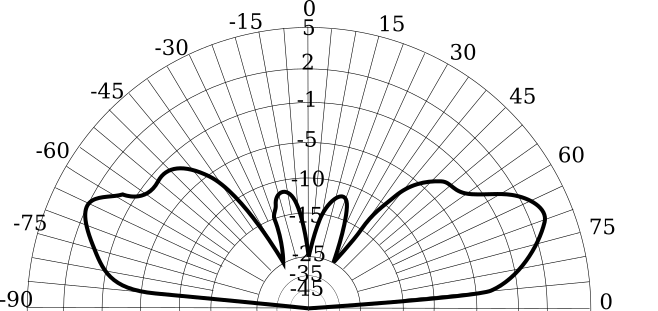
\includegraphics[width=1\linewidth]{r8_25_5x7.png} \\ b)}
\end{minipage}
\caption{Вертикальный план диаграммы направленности одиночного излучателя (a) и ФАР 5:7 (b) при 25МГц}
\label{ris:f25mhs}
\end{figure}

Интересный результат наблюдается при 25МГц (см~Рис.~\ref{ris:f25mhs}), где усиление ФАР существенно больше усиления одиночного излучателя. Сравнение их диаграмм направленности показывает, что одиночный излучатель довольно плохо излучает в направлении оптимизации, тогда как ФАР имеет максимум излучения в этом направлении. Невозможно было бы достигнуть такого явления без учета взаимного влияния. Отсюда следует, что при оптимизации направленности ФАР КВ диапазона не следует пренебрегать взаимным влиянием, поскольку это может существенно изменить вид диаграммы направленности.

Далее рассмотрим как горизонтальный план диаграммы направленности меняется с ростом частоты~(см. рис.~\ref{ris:horizontal}). Направление оптимизации - $45^{\circ}$. Здесь мы можем наблюдать, что при частоте, равной 5МГц, диаграмма направленности представляется почти овальной формой. Дальнейшее увеличение частоты до 15МГц приводит диаграмму направленности к очень направленной форме. Затем увеличение частоты ведет к довольно сложной форме, при которой максимум излучения становится менее ярко выражен.

\begin{figure}
\begin{minipage}[h]{0.49\linewidth}
\center{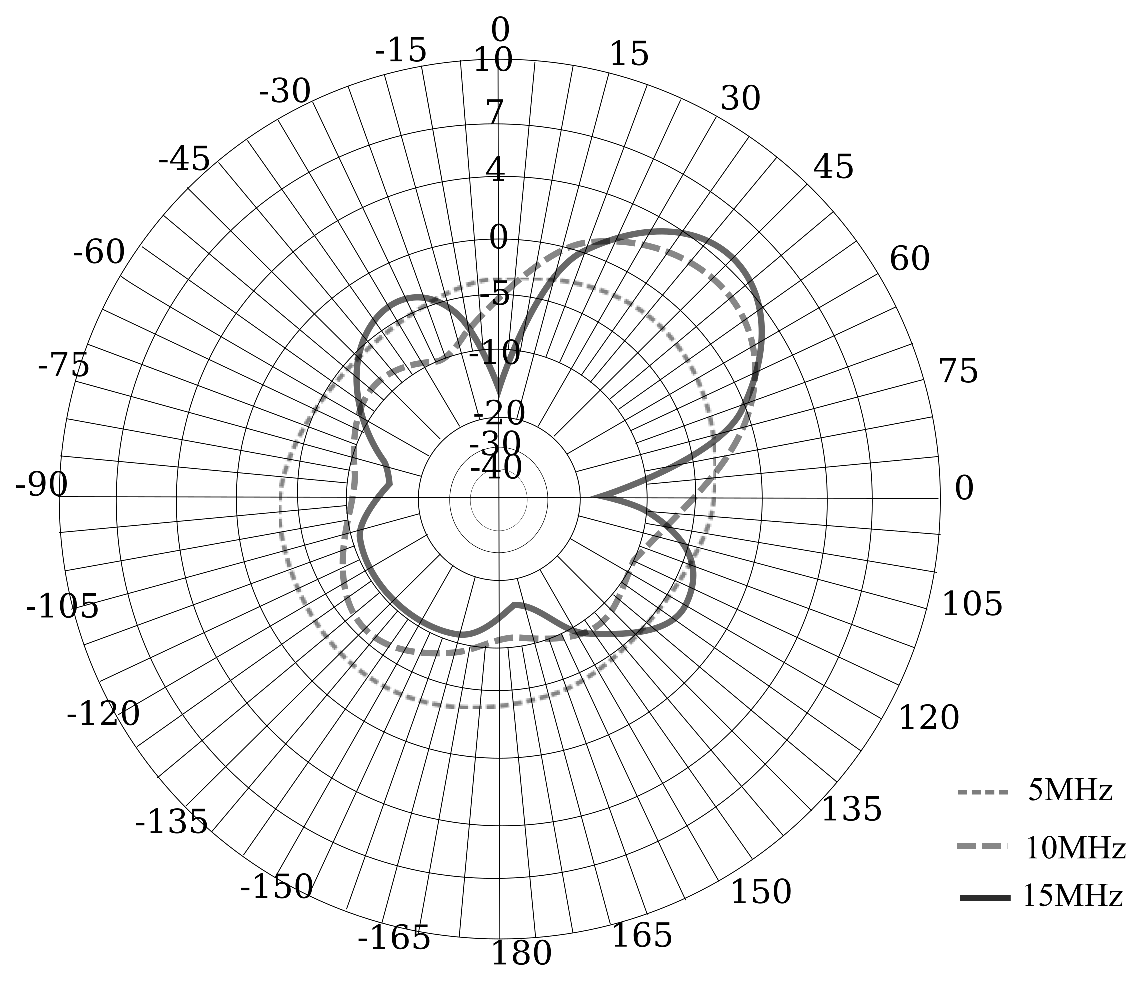
\includegraphics[width=1\linewidth]{r8_horizontal_5x7.eps} \\ a)}
\end{minipage}
\hfill
\begin{minipage}[h]{0.49\linewidth}
\center{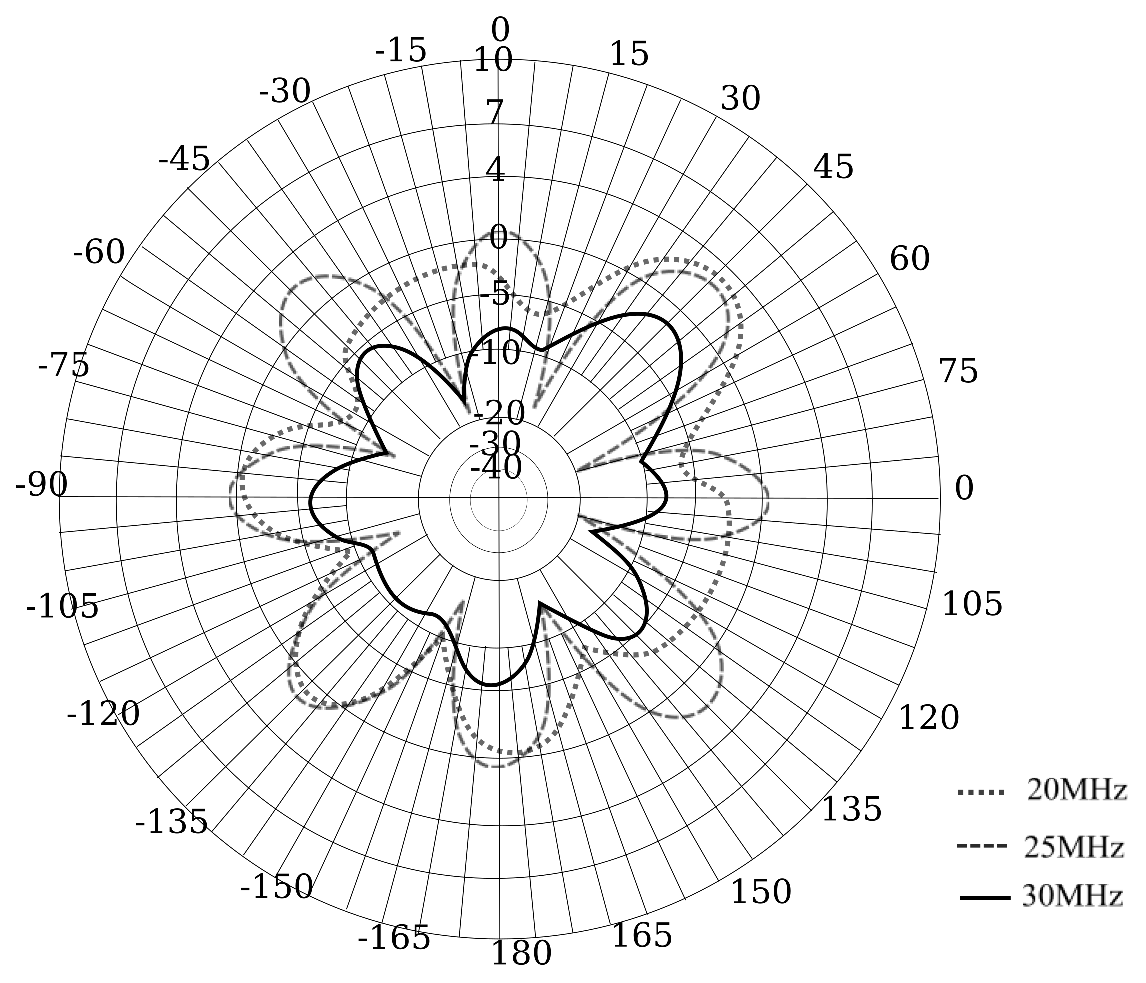
\includegraphics[width=1\linewidth]{r8_horizontal_5x7_2.eps} \\ b)}
\end{minipage}
\caption{Горизонтальный план диаграммы направленности для ФАР 5:7 5-15МГц (a) и 20-30МГц (b)}
\label{ris:horizontal}
\end{figure}

\section{Исследование взаимного влияния излучателей} 

Все эксперименты проводились при реальной земле, рассчитанной по методу Зоммерфельда-Нортона пакетом NEC-2. Для проведения эксперимента было выбрано несколько частот в рабочем диапазоне, однако, все приведенные в данной статье результаты приходятся на 5 МГц, поскольку именно эти результаты носят наиболее иллюстративный характер.
Рассмотрим случай фазирования решетки без учета взаимного влияния ее элементов. Для этого обратимся к формуле~(\ref{eq:A}). Если пренебречь взаимным влиянием излучателей, плотность мощности $F$ будет максимальна тогда, когда комплексные амплитуды парциальных полей будут синфазны. В данной работе производилось сравнение диаграмм направленности решеток разных конфигураций после математической оптимизации их направленности в заданном направлении согласно модели~(\ref{eq:task3}) с соответствующими диаграммами одиночного излучателя и со случаем фазирования решетки без учета взаимного влияния (далее – простое фазирование).
Для проведения вычислительного эксперимента использовался решатель BARON в пакете GAMS, поскольку, как правило, он обеспечивает бо́льшую точность решений по сравнению с градиентным подъемом. Высота каждого ШВИ равна 15 м. Длина плеча симметричных излучателей также равна 15 м.
Каждая кольцевая решетка состоит из восьми излучателей. Направление оптимизации по умолчанию было установлено на $70^{\circ}$ полярного угла и $45^\circ$ азимутального угла в сферических координатах. Для некоторых экспериментов было проведено дополнительное исследование при $85^\circ$ полярного угла.


\subsection{Широкополосные вертикальные излучатели} 
В рамках данного эксперимента производилось сравнение диаграмм направленности при варьировании расстояния центра излучателя до центра решетки (от 7 до 80 м.), длины радиальных противовесов (от 3 до 20 м.) и присутствия или отсутствия общей системы противовесов. Диаграммы направленности при этом имели различную форму, однако, качественно различие между коэффициентами усиления всегда сохранялось (см.~рис.~\ref{ris:bve_mut}): результат оптимизации не дает значимого преимущества перед простым фазированием.  Модули диагональных и недиагональных элементов матрицы проводимостей в указанном примере не превосходили 0.002 и 0.0003 См соответственно.

\begin{figure}
\begin{minipage}[h]{0.49\linewidth}
\center{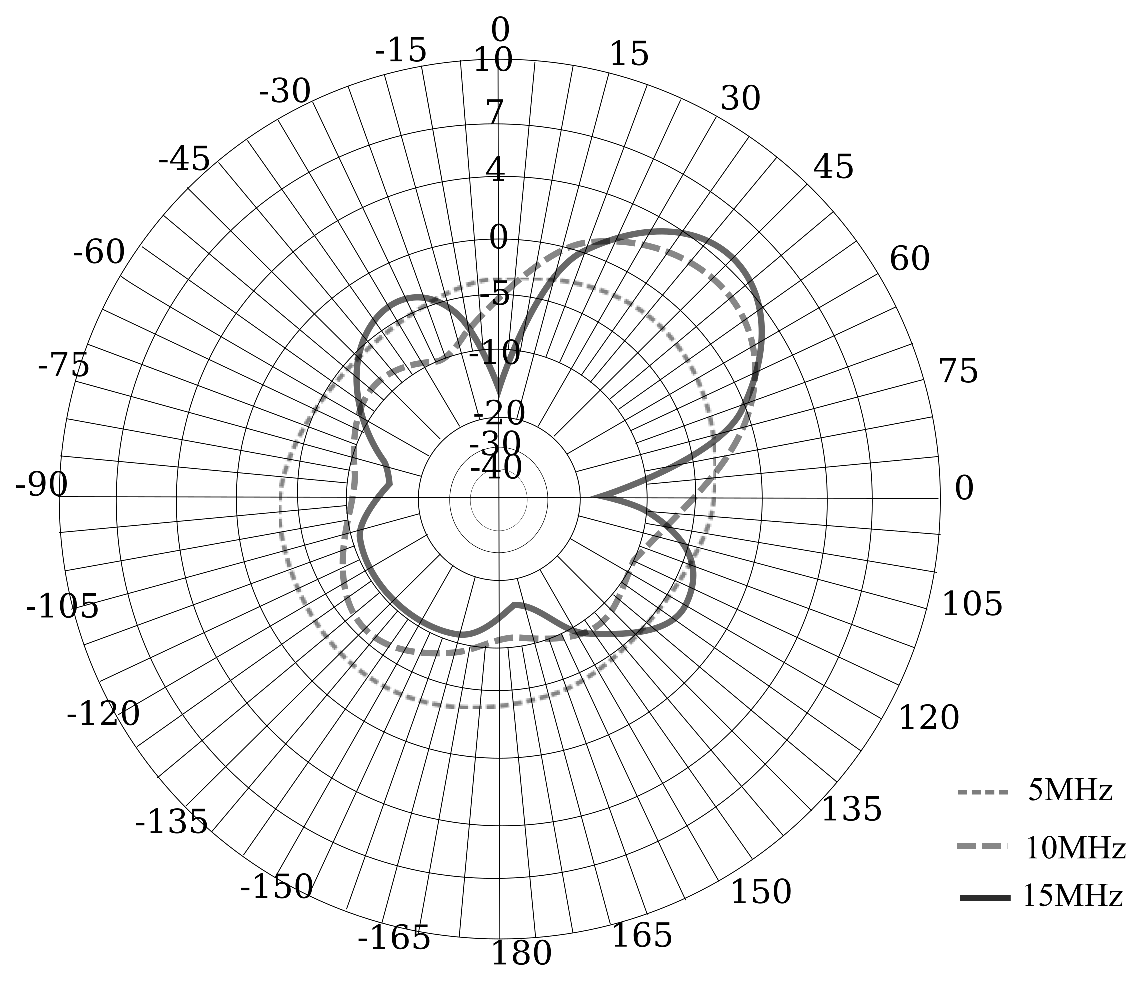
\includegraphics[width=1\linewidth]{r8_horizontal_5x7.eps} \\ a)}
\end{minipage}
\hfill
\begin{minipage}[h]{0.49\linewidth}
\center{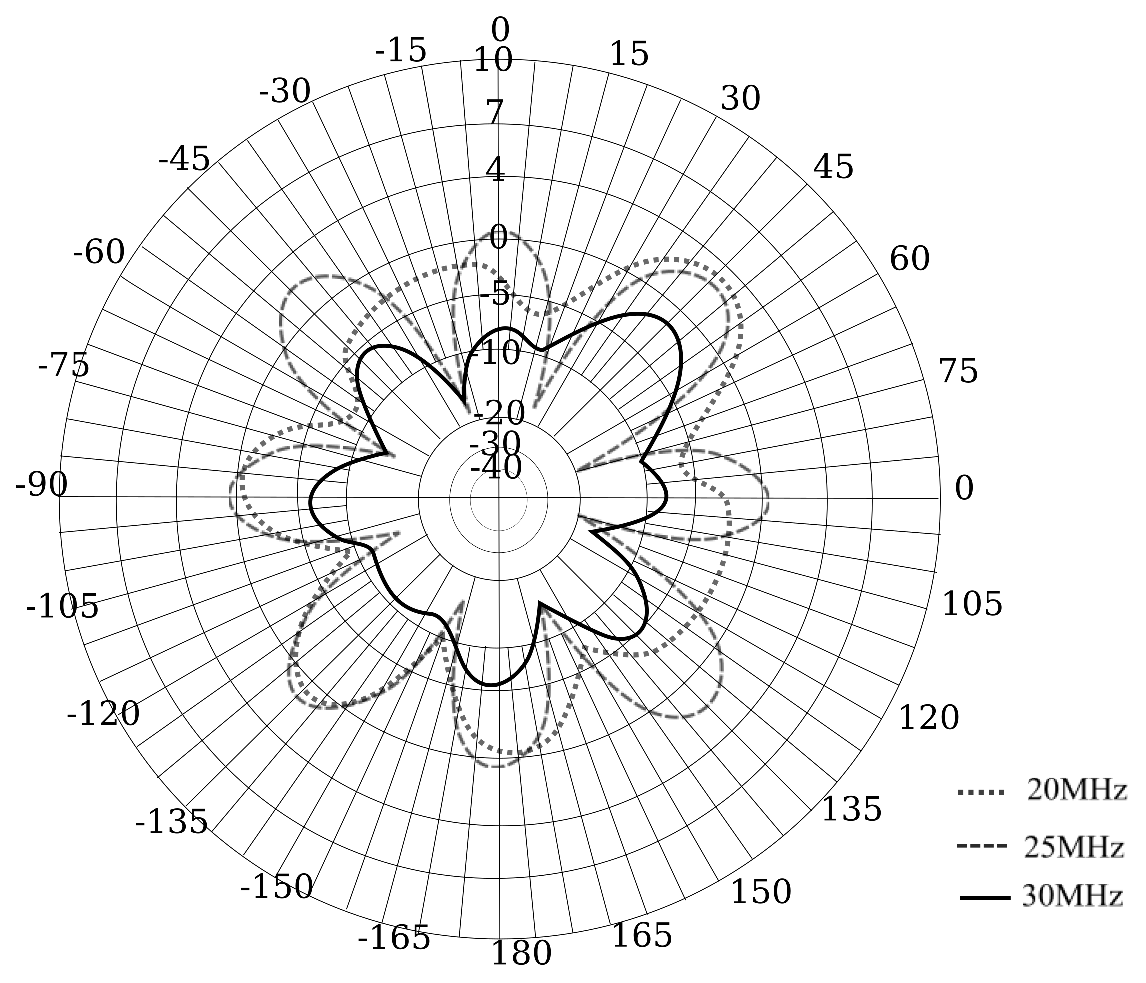
\includegraphics[width=1\linewidth]{r8_horizontal_5x7_2.eps} \\ b)}
\end{minipage}
\caption{Горизонтальная (a) и вертикальная (b) плоскость диаграммы направленности ШВИ при расстоянии от центра излучателя до центра решетки 15 м. и длиной радиальных противовесов 5 м. Пунктирной линией обозначено усиление одиночного излучателя, штрихпунктирной--простое фазирование, сплошной--решение задачи мат. программирования.}
\label{ris:bve_mut}
\end{figure}

\subsection{Симметричные излучатели}
Для ШВД производилось исследование диаграмм направленности при варьировании расстояния центра излучателя до центра решетки от 5 до 50 м. В большинстве случаев, использование решения задачи математического программирования не давало существенного преимущества перед простым фазированием (см. рис. 4). Модули диагонального и недиагонального элементов матрицы проводимостей в приведенном примере не превосходили 0.016 и 0.006 См соответственно.   Тем не менее, при расстоянии между центром излучателя и центром решетки равным 20 м. это различие составило около 4 дБ (см. рис. 5). Здесь модули диагональных и недиагональных элементов матрицы проводимостей не превосходили 0.013 и 0.008 См соответственно.

\begin{figure}
\begin{minipage}[h]{0.49\linewidth}
\center{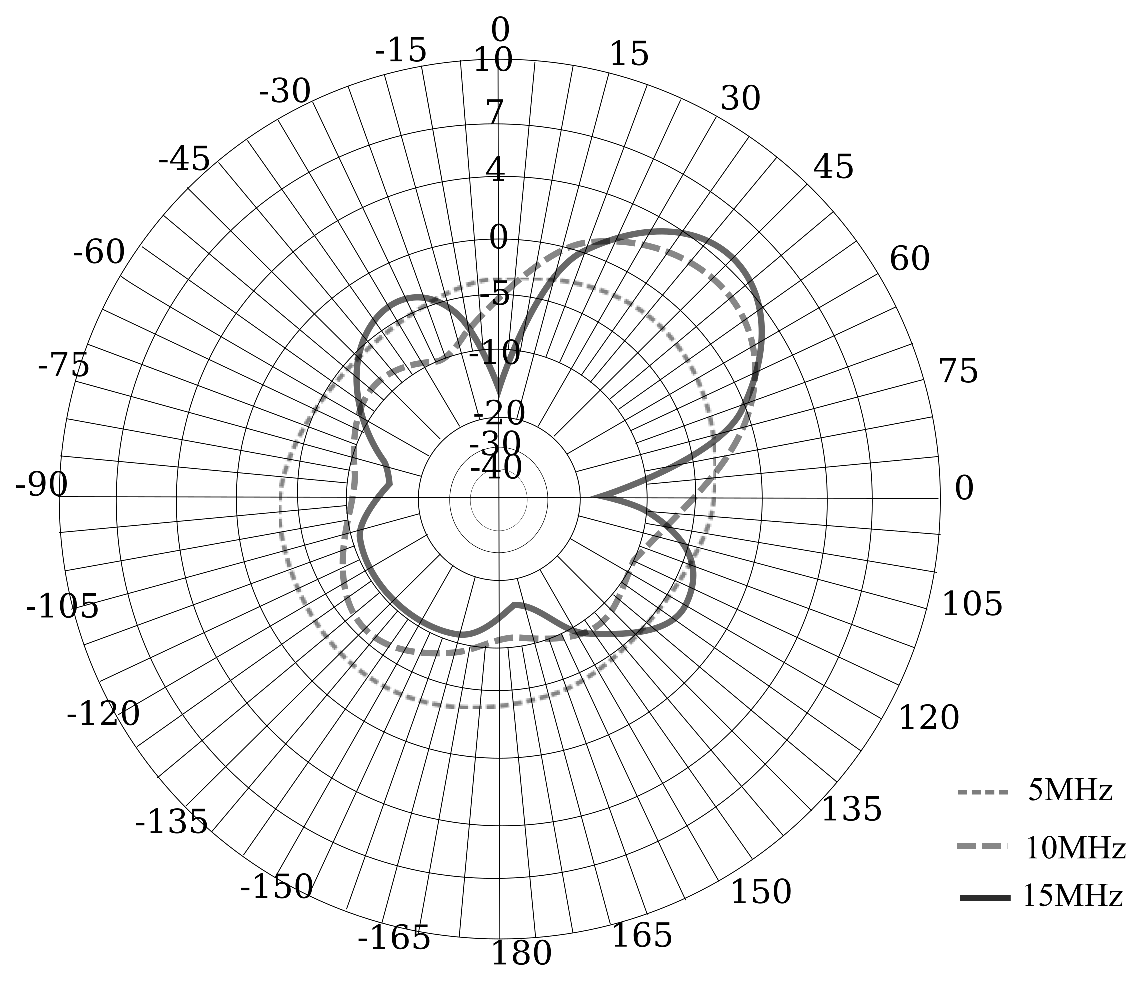
\includegraphics[width=1\linewidth]{r8_horizontal_5x7.eps} \\ a)}
\end{minipage}
\hfill
\begin{minipage}[h]{0.49\linewidth}
\center{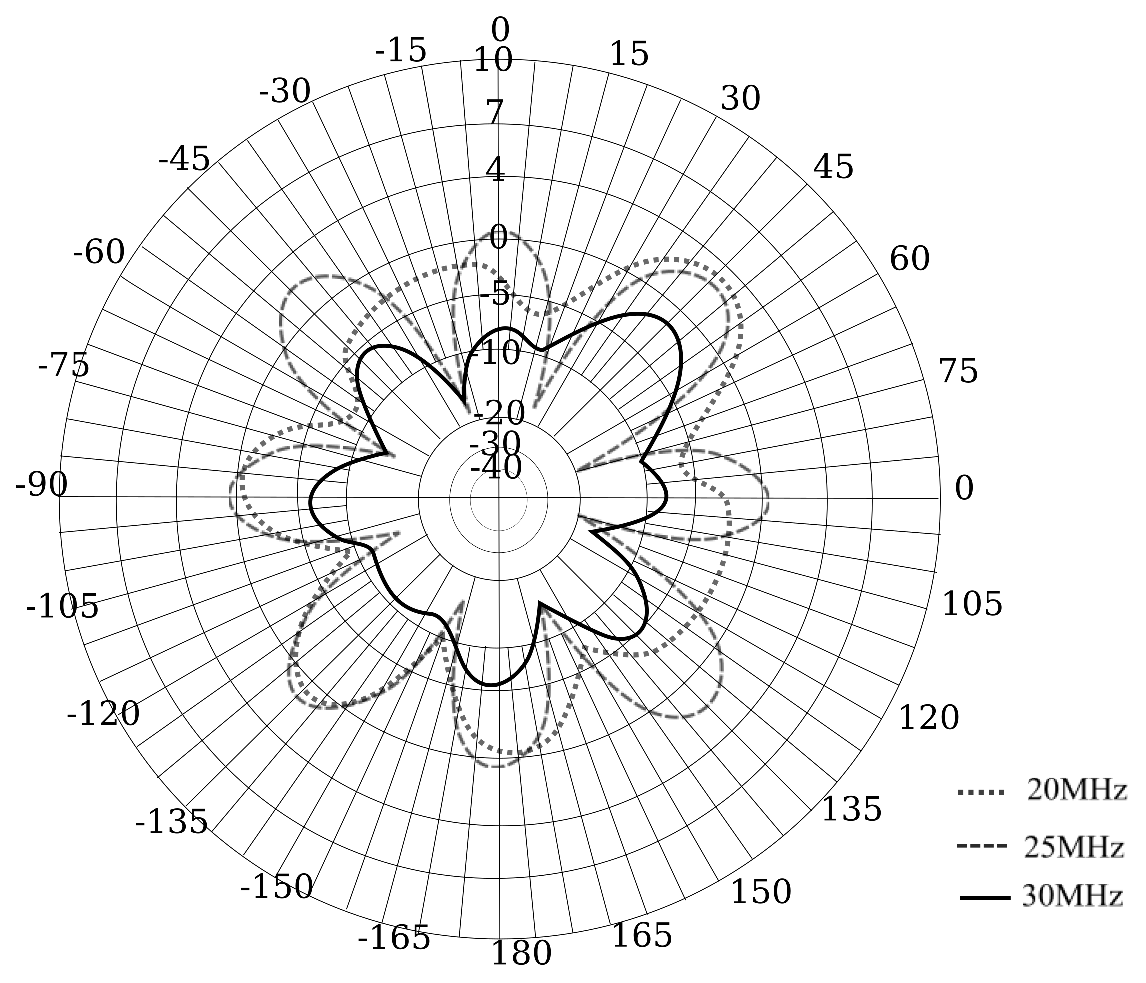
\includegraphics[width=1\linewidth]{r8_horizontal_5x7_2.eps} \\ b)}
\end{minipage}
\caption{Горизонтальная (a) и вертикальная (b) плоскость диаграммы направленности ШВД при расстоянии от центра излучателя до центра решетки 30 м. Пунктирной линией обозначено усиление одиночного излучателя, штрихпунктирной--простое фазирование, сплошной--решение задачи мат. программирования.}
\label{ris:bve_mut}
\end{figure}

\begin{figure}
\begin{minipage}[h]{0.49\linewidth}
\center{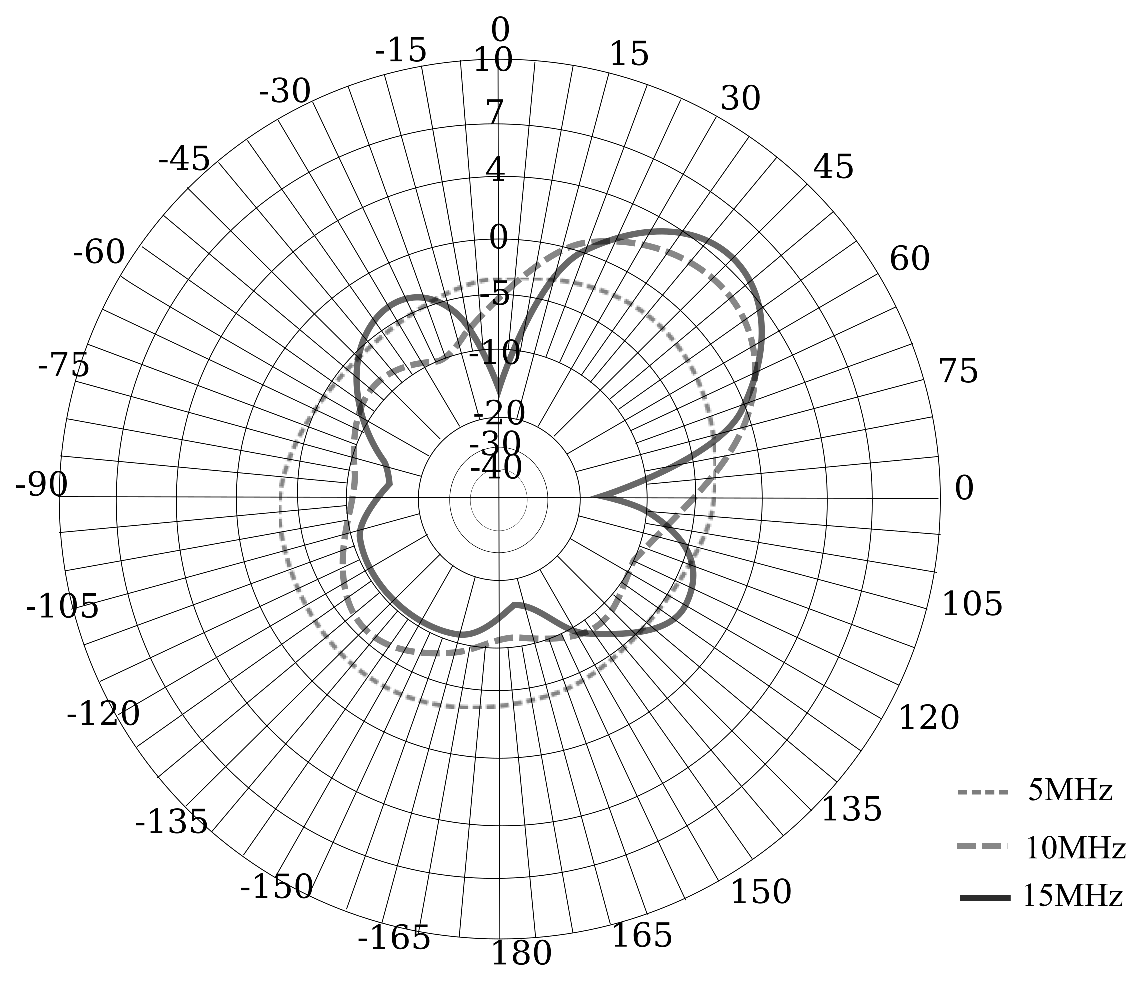
\includegraphics[width=1\linewidth]{r8_horizontal_5x7.eps} \\ a)}
\end{minipage}
\hfill
\begin{minipage}[h]{0.49\linewidth}
\center{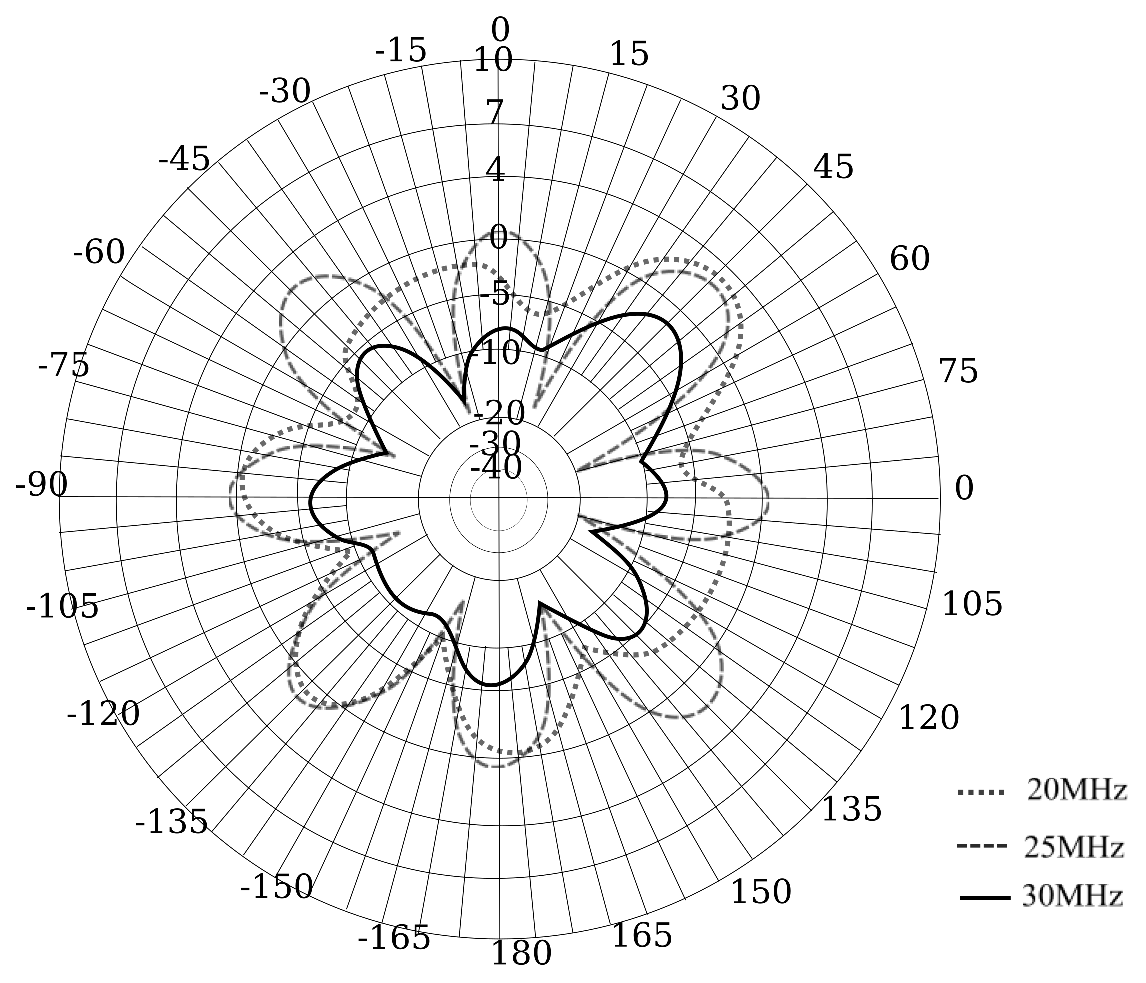
\includegraphics[width=1\linewidth]{r8_horizontal_5x7_2.eps} \\ b)}
\end{minipage}
\caption{Горизонтальная (a) и вертикальная (b) плоскость диаграммы направленности ШВД при расстоянии от центра излучателя до центра решетки 20 м. Пунктирной линией обозначено усиление одиночного излучателя, штрихпунктирной--простое фазирование, сплошной--решение задачи мат. программирования.}
\label{ris:bve_mut}
\end{figure}

Аналогичные результаты были получены и для решетки СВД (см. рис. 5). При оптимизации в направлении полярного угла равном $70^{\circ}$ при варьировании расстояния от центра излучателя до центра решетки от 35 до 37 м. разница между коэффициентом усиления решения задачи математического программирования и усилением простого фазирования также достигала 4 дБ. При этом модули диагональных и недиагональных элементов матрицы проводимостей не превосходили 0.033 и 0.021 См соответственно.  При оптимизации в направлении полярного угла равном $85^{\circ}$ при варьировании расстояния от центра излучателя до центра решетки от 25 до 29 м. эта разница достигала 5 дБ.(см. рис. 6). Здесь модули диагональных и недиагональных элементов матрицы проводимостей примере не превосходили 0.015 и 0.009 См соответственно.

\begin{figure}
\begin{minipage}[h]{0.49\linewidth}
\center{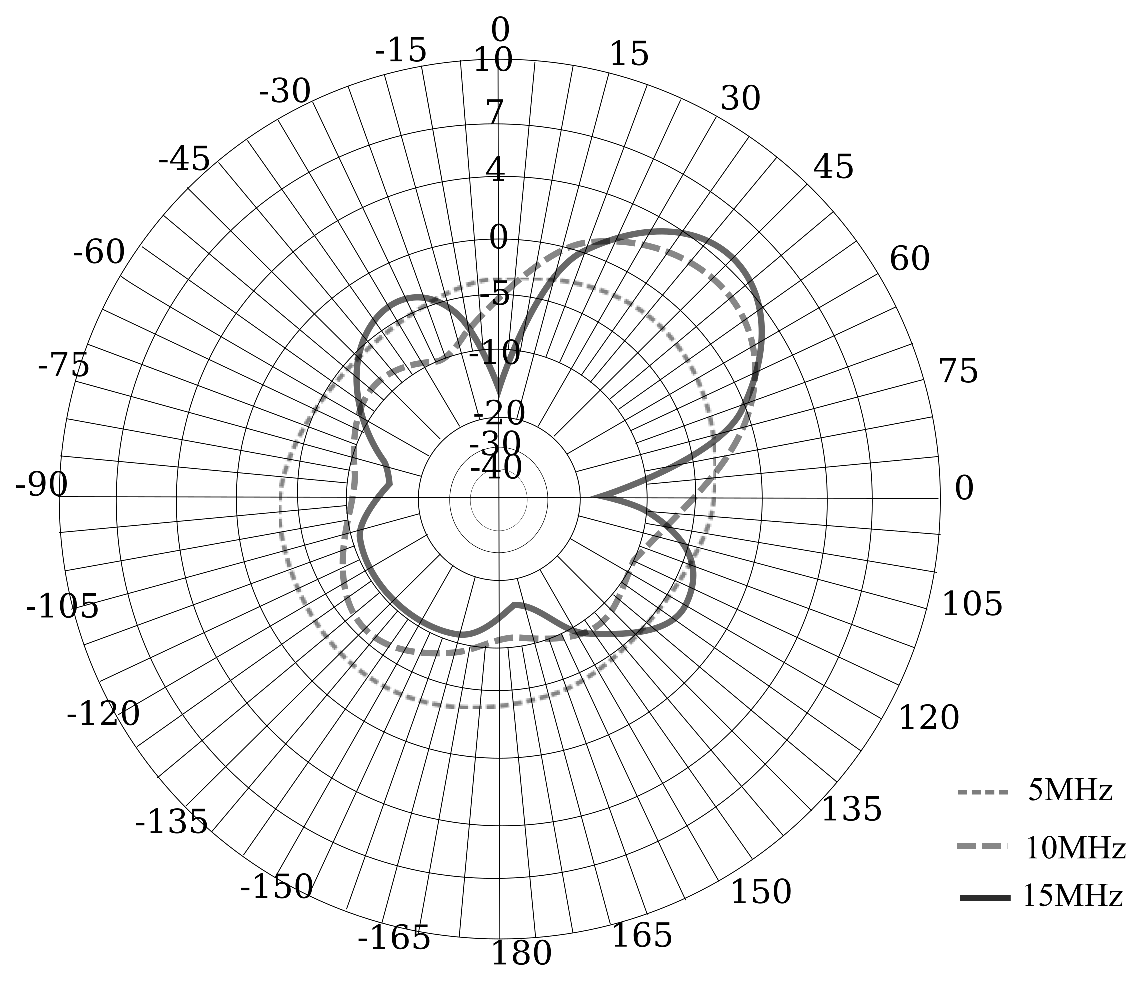
\includegraphics[width=1\linewidth]{r8_horizontal_5x7.eps} \\ a)}
\end{minipage}
\hfill
\begin{minipage}[h]{0.49\linewidth}
\center{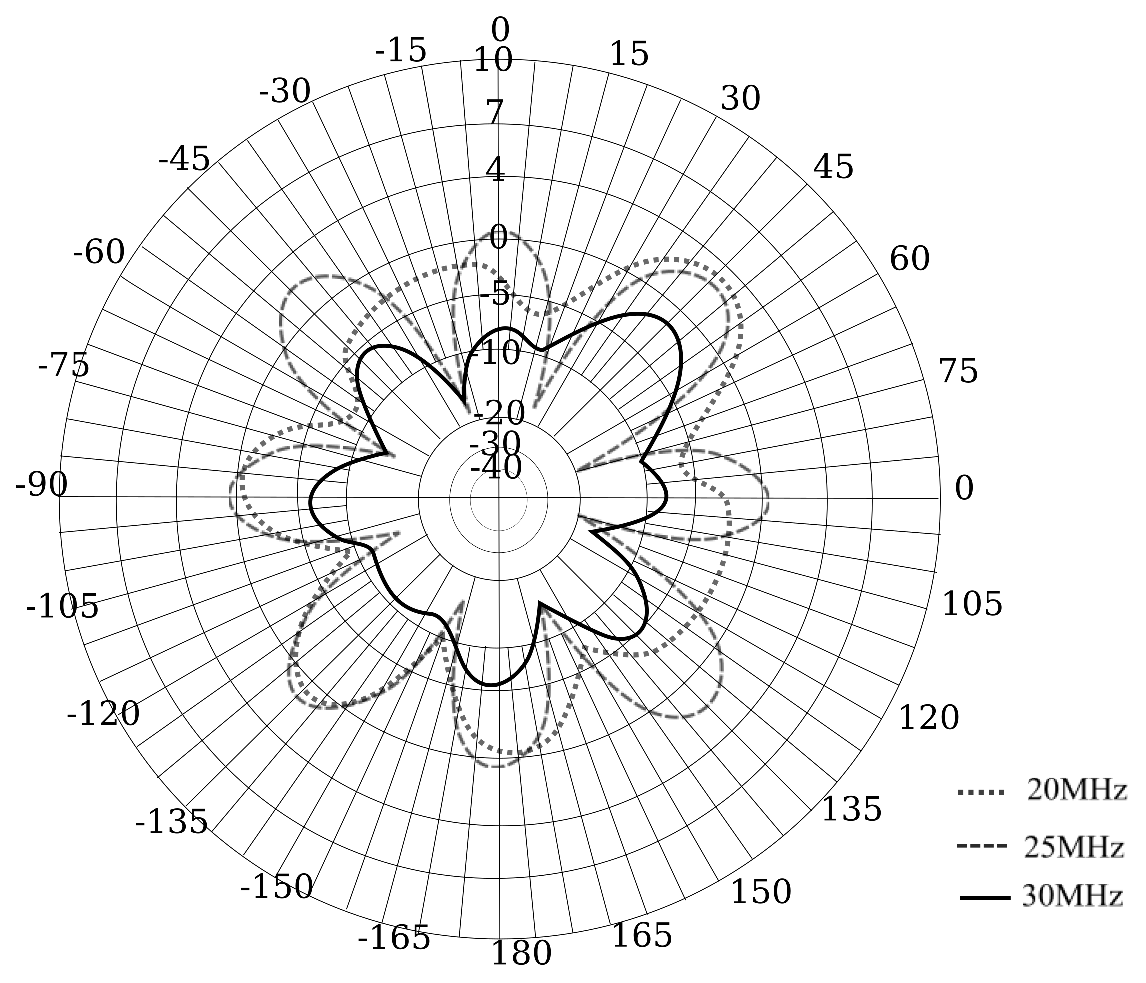
\includegraphics[width=1\linewidth]{r8_horizontal_5x7_2.eps} \\ b)}
\end{minipage}
\caption{Горизонтальная (a) и вертикальная (b) плоскость диаграммы направленности СВД при расстоянии от центра излучателя до центра решетки 37 м. Пунктирной линией обозначено усиление одиночного излучателя, штрихпунктирной--простое фазирование, сплошной--решение задачи мат. программирования.}
\label{ris:bve_mut}
\end{figure}

\begin{figure}
\begin{minipage}[h]{0.49\linewidth}
\center{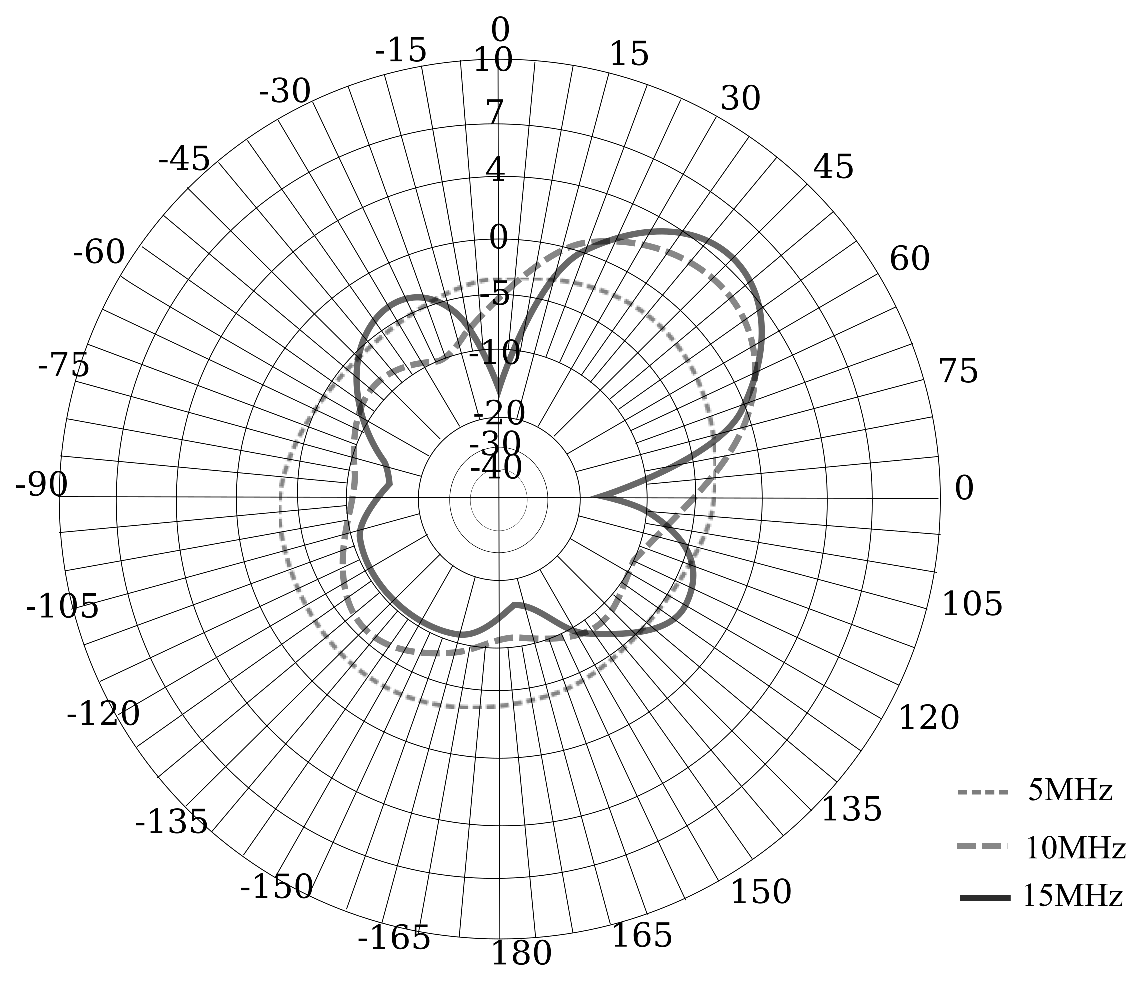
\includegraphics[width=1\linewidth]{r8_horizontal_5x7.eps} \\ a)}
\end{minipage}
\hfill
\begin{minipage}[h]{0.49\linewidth}
\center{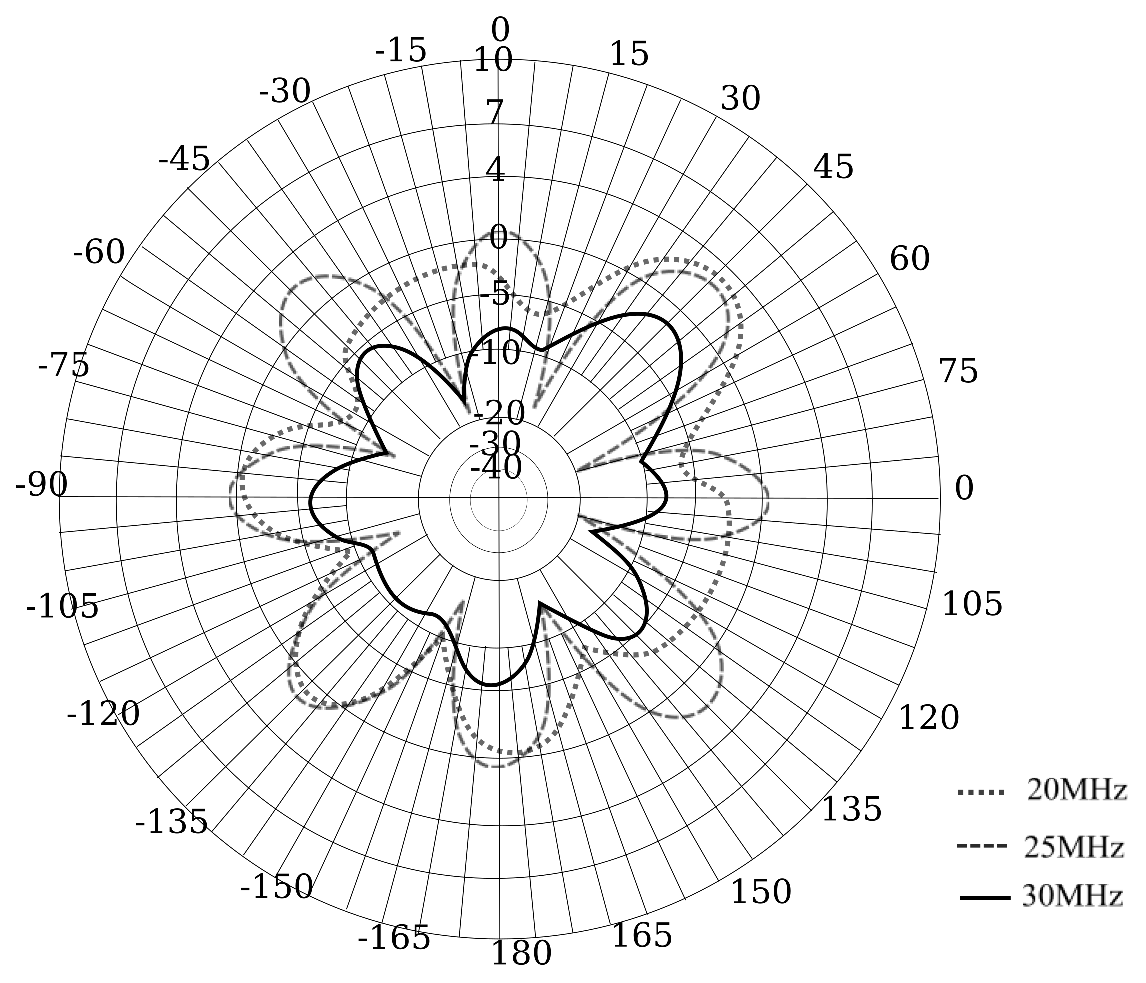
\includegraphics[width=1\linewidth]{r8_horizontal_5x7_2.eps} \\ b)}
\end{minipage}
\caption{Горизонтальная (a) и вертикальная (b) плоскость диаграммы направленности СВД при расстоянии от центра излучателя до центра решетки 25 м, полученные для $85^{\circ}$ полярного угла. Пунктирной линией обозначено усиление одиночного излучателя, штрихпунктирной--простое фазирование, сплошной – решение задачи мат. программирования.}
\label{ris:bve_mut}
\end{figure}

\subsection{Интерпретация результатов экспериментов по исследованию взаимного влияния излучателей}
В рамках данного исследования было выявлено наличие ситуаций, в которых коэффициент усиления, соответствующий решению задачи математического программирования, имеет существенное преимущество перед коэффициентом усиления простого фазирования. Например, при оптимизации в направлении ($70^{\circ}$, $45^\circ$) в случае ШВД при расстоянии излучателя до центра решетки равном 20 м. и СВД при расстоянии излучателя до центра решетки равном 37 м. разница составляет порядка 4 дБ. При оптимизации в направлении ($85^\circ$, $45^{\circ}$) в случае СВД  при расстоянии излучателя до центра решетки равном 25 м. эта разница достигает 5 дБ. Следовательно, при оптимизации направленности ФАР КВ диапазона целесообразны расчеты с учетом взаимного влияния излучателей. В то же время, отмечены случаи, когда результат решения задачи математического программирования не дает существенного прироста усиления по сравнению с фазированием без учета взаимного влияния.
Использование ШВИ в качестве излучателей ФАР КВ диапазона выглядит малоприменимым, поскольку требуют чрезмерно сложной системы противовесов.

\chapter*{Заключение}                       % Заголовок
\addcontentsline{toc}{chapter}{Заключение}  % Добавляем его в оглавление

%% Согласно ГОСТ Р 7.0.11-2011:
%% 5.3.3 В заключении диссертации излагают итоги выполненного исследования, рекомендации, перспективы дальнейшей разработки темы.
%% 9.2.3 В заключении автореферата диссертации излагают итоги данного исследования, рекомендации и перспективы дальнейшей разработки темы.
%% Поэтому имеет смысл сделать эту часть общей и загрузить из одного файла в автореферат и в диссертацию:

Основные результаты работы заключаются в следующем.
%% Согласно ГОСТ Р 7.0.11-2011:
%% 5.3.3 В заключении диссертации излагают итоги выполненного исследования, рекомендации, перспективы дальнейшей разработки темы.
%% 9.2.3 В заключении автореферата диссертации излагают итоги данного исследования, рекомендации и перспективы дальнейшей разработки темы.
\begin{enumerate}
  \item В текущей работе была рассмотрена постановка задачи оптимизации направленности излучения антенной системы, представленной в виде регулярной решетки излучателей. Для данной задачи была разработана модель квадратичного программирования в вещественных числах. Произведено сравнение результатов разработанных алгоритмов в вычислительном эксперименте.
  \item Проведены вычислительные эксперименты, выявляющие наличие непрерывных групп симметрий допустимых решений. Для всех рассмотренных задач выявлено наличие только фазовой симметрии.
  \item В рамках данного исследования было выявлено наличие ситуаций, в которых коэффициент усиления, соответствующий решению задачи математического программирования, имеет существенное преимущество перед коэффициентом усиления простого фазирования. Выявлено, что, при оптимизации направленности ФАР КВ диапазона целесообразны расчеты с учетом взаимного влияния излучателей.
  \item Для генерации тестовых примеров, автоматизации вычислительных экспериментов и визуализации их результатов были разработаны интерпретатор <<Expi>> и его графическая оболочка <<ExpiIDE>>.
\end{enumerate}


В заключение автор выражает благодарность и большую признательность научному руководителю
Еремееву~А.\,В. за поддержку, помощь, обсуждение результатов и~научное
руководство. Особую благодарность автор выражает Юркову~А.\,С. за консультации по радиотехническим аспектам работы, помощь в организации вычислительных экспериментов и интерпретации полученных результатов. Также автор благодарит авторов шаблона
*Russian-Phd-LaTeX-Dissertation-Template* за~помощь в оформлении
диссертации.

Исследование выполнено при финансовой поддержке Российского фонда фундаментальных исследований (проект №~19--37--90066/19)      % Заключение
\printnomenclature[3.5cm] % Значение ширины столбца с обозначениями стоит подбирать вручную
        % Список сокращений и условных обозначений
\chapter*{Словарь терминов}             % Заголовок
\addcontentsline{toc}{chapter}{Словарь терминов}  % Добавляем его в оглавление

\textbf{Фазированная антенная решетка (ФАР)} : антенная система, представляющая собой регулярную решетку излучателей, соединенных со специальными устройствами, обеспечивающими распределение фаз и амплитуд в излучателях для получения направленного излучения

\textbf{ВЧ (КВ) диапазон} : диапазон радиоволн с частотой от 3 МГц (длина волны 100 м) до 30 МГц (длина волны 10 м)
\textbf{СВЧ (УКВ) диапазон} : диапазон радиоволн с частотой от 30 МГц (длина волны 10 м) до 3000 ГГц (длина волны 0.1 мм)
      % Словарь терминов
\clearpage                                  % В том числе гарантирует, что список литературы в оглавлении будет с правильным номером страницы
%\hypersetup{ urlcolor=black }               % Ссылки делаем чёрными
%\providecommand*{\BibDash}{}                % В стилях ugost2008 отключаем использование тире как разделителя
\urlstyle{rm}                               % ссылки URL обычным шрифтом
\ifdefmacro{\microtypesetup}{\microtypesetup{protrusion=false}}{} % не рекомендуется применять пакет микротипографики к автоматически генерируемому списку литературы
\insertbibliofull                           % Подключаем Bib-базы: все статьи единым списком
% Режим с подсписками
%\insertbiblioexternal                      % Подключаем Bib-базы: статьи, не являющиеся статьями автора по теме диссертации
% Для вывода выберите и расскомментируйте одно из двух
%\insertbiblioauthor                        % Подключаем Bib-базы: работы автора единым списком 
%\insertbiblioauthorgrouped                 % Подключаем Bib-базы: работы автора сгруппированные (ВАК, WoS, Scopus и т.д.)
\ifdefmacro{\microtypesetup}{\microtypesetup{protrusion=true}}{}
\urlstyle{tt}                               % возвращаем установки шрифта ссылок URL
%\hypersetup{ urlcolor={urlcolor} }          % Восстанавливаем цвет ссылок
      % Список литературы
\chapter*{ПРИЛОЖЕНИЯ}
\addcontentsline{toc}{chapter}{ПРИЛОЖЕНИЯ}
\section*{Приложение А}\label{sec:applic_a}
\addcontentsline{toc}{section}{Приложение A}
Здесь приводится подробное описание алгоритма исследования структуры локальных оптимумов. Для удобства изложения, алгоритм разбит
на процедуры: <<Одномерный поиск>>, <<Градиентный подъем>> и <<Исследование локальных оптимумов>>.
\\ \\
\noindent{\textbf{ 1. Одномерный поиск.}}

\noindent{\textbf{ Дано:}}
\begin{itemize}
  \item вектор начального решения $\textbf{x}$ размерности $2N$,
  \item вектор направления одномерного поиска $\textbf{d}$ размерности $2N$,
  \item точность вычислений $\epsilon_{1dim}$.
\end{itemize}
\noindent{\textbf{ Требуется:}} найти вектор $\textbf{x}' = \textbf{x} + \gamma \textbf{d}$ такой, что
\begin{itemize}
  \item $\tilde{F}(\textbf{x}) < \tilde{F}(\textbf{x}'),$
  \item $\tilde{F}(\textbf{x} + (\gamma + \epsilon_{1dim}) \textbf{d}) < \tilde{F}(\textbf{x}').$
\end{itemize}
\begin{enumerate}
  \item Инициализировать параметр одномерного поиска $\beta := 1$, вектор $\textbf{x}' := \textbf{x}$, счетчик итераций $j := 1$.
  \item Если $\tilde{F}(\textbf{x}' + \beta \textbf{d}) < \tilde{F}(\textbf{x}')$, то уменьшить $\beta := \beta / 2$.
  В противном случае, в зависимости от значения счетчика:\\
  при $j = 1$ положить $\textbf{x}_a := \textbf{x}'$,\\
  при $j = 2$ положить $\textbf{x}_b := \textbf{x}'$,\\
  при $j = 3$ положить $\textbf{x}_c := \textbf{x}'$,\\
  при $j > 3$ положить $\textbf{x}_a := \textbf{x}_b$, $\textbf{x}_b := \textbf{x}_c$, $\textbf{x}_c := \textbf{x}'$.\\
  При этом, вне зависимости от значений счетчика, $\beta := 2\beta$,\\
  $\textbf{x}' := \textbf{x}' + \beta \textbf{d}.$
  \item Если $\beta < \epsilon_{1dim}$ и $j < 3$, вернуть $\textbf{x}'$.
  \item Если $\beta < \epsilon_{1dim}$ и $j \geq 3$, то переходим к шагу 5, иначе - на шаг 2.
  \item По точкам $\textbf{x}_a, \textbf{x}_b, \textbf{x}_c$ строим квадратичную аппроксимацию:
   $$\textbf{x}^{*} := (\textbf{x}_b - 3 \beta \textbf{d}) +
   \left(\beta\left(1 + \frac{\tilde{F}(\textbf{x}_a) - \tilde{F}(\textbf{x}_c)}{2(\tilde{F}(\textbf{x}_a) -
   2\tilde{F}(\textbf{x}_b) + \tilde{F}(\textbf{x}_c))}\right)\right)\textbf{d}.$$\\
\end{enumerate}
{ \textbf{2. Градиентный подъем.}}
\\ \\
\noindent{\textbf{Дано:}}
\begin{itemize}
  \item вектор начального решения $\textbf{x}_0$ размерности $2N$,
  \item точность вычислений $\epsilon_{grad}$,
  \item точность вычислений одномерного поиска $\epsilon_{1dim}$,
  \item время принудительного завершения работы алгоритма $time_{finish}.$\\
\end{itemize}
\noindent{\textbf{Требуется:}} найти вектор $\textbf{x}$ такой, что
для всех $$\textbf{d}, |\textbf{d}| = 1 \text{~выполняется~} \tilde{F}(\textbf{x} + (\epsilon_{grad})\textbf{d}) < \tilde{F}(\textbf{x})$$.\\
\begin{enumerate}
  \item $\textbf{x} := \textbf{x}_0.$
  \item Вычислить и нормировать градиент целевой функции:
   $$\textbf{d} := \frac{\nabla \tilde{F}(\textbf{x})}{|\nabla \tilde{F}(\textbf{x})|}.$$
  \item Вычислить $\textbf{x}^{*}$ алгоритмом одномерного поиска~1 с параметрами $\textbf{x}, \textbf{d}, \epsilon_{1dim}.$
  \item Записать в $time$ текущее время. Если $time \geq time_{finish}$, вернуть $\textbf{x}^{*}$.
  \item Если $|\tilde{F}(\textbf{x}) - \tilde{F}(\textbf{x}^{*})| < \epsilon_{grad}$, вернуть $\textbf{x}^{*}$, иначе положить $\textbf{x} = \textbf{x}^{*}$ и повторить~шаги~2-5.\\ \\
\end{enumerate}

\noindent{\textbf{ 3. Исследование локальных оптимумов.}}
\\ \\
\noindent{\textbf{Дано:}}
\begin{itemize}
  \item $x_{\max}$ как верхняя оценка нормы допустимой области,
  \item точность вычислений $\epsilon_{grad}$,
  \item точность вычислений одномерного поиска $\epsilon_{1dim}$,
  \item время принудительного завершения работы алгоритма $time_{finish}$,
  \item максимально допустимая норма вектора ${\textbf{y}}$, обозначаемая за ${\textbf{y}}_{\max}$.\\
\end{itemize}

\noindent{\textbf{Требуется:}} провести исследование структуры локальных оптимумов, как описано в разделе~\ref{sec:exp}.\\

\begin{enumerate}
  \item Инициализировать каждую компоненту начального вектора $x_{0,i = \overline{1,2N}}$ равномерно распределенной в интервале $[-x_{\max}, x_{\max}]$
  величиной.
  \item Вычисляем допустимый вектор $\textbf{x}$ путем масштабирования $\textbf{x}_0$ в допустимую область:
  $$\textbf{x} := (\max_{k=\overline{1,n}} {\textbf{x}_0}^T \textbf{H}^{(k)}{\textbf{x}_0})^{-1/2} {\textbf{x}_0}.$$
  \item Вычислить ${\textbf{x}^{*}}$ алгоритмом градиентного подъема~(2) с параметрами ${\textbf{x}}, \epsilon_{grad}, \epsilon_{1dim}, time_{finish}.$
  \item Записать в $time$ текущее время. Если $time$ < $time_{finish}$, перейти на шаг~1.
  \item Для каждого найденного решения установить ${\textbf{x}_0^{*}} = {\textbf{x}^{*}}$, составить линеаризованную задачу~(\ref{eq:task5}) и найти
  ее решение ${\textbf{x}_{lp}^{*}}$.
  \item Исключить решения, для которых $|{\textbf{x}_0^{*}} - {\textbf{x}_{lp}^{*}}| > {\textbf{y}_{\max}}$. В случае оставшихся решений установить
  $\textbf{x} = {\textbf{x}_{lp}^{*}}$ и повторить шаги~2-3. Оценить норму разницы $|{\textbf{x}_0^{*}} - {\textbf{x}^{*}}|$. Вернуть ${\textbf{x}_0^{*}}$ с
  лучшим значением $\tilde{F}({\textbf{x}_0^{*}})$ в качестве результата.
\end{enumerate}

\section*{Приложение Б}
\addcontentsline{toc}{section}{Приложение Б}
\label{sec:applic_b}
Комплекс моделирования и решения задач оптимизации направленности ФАР КВ диапазона <<Expi>> предназначен для моделирования антенных систем и вычисления управляющих параметров фазированных антенных решеток (ФАР).Регистрируемая программа для ЭВМ применима в радиотехнике
при оптимизации направленного излучения ФАР КВ диапазона.Программа позволяет запускать файлы заданного формата с инструкциями по организации вычислительного эксперимента, редактировать их, визуализировать результаты.
Здесь приводится графический интерфейс и функциональные возможности разработанного в рамках текущей работы программного комплекса <<Expi>>.

\subsection*{Графический интерфейс}
  Программное окно разделено на три части: обозреватель текущей директории, окно вывода и рабочая область. Содержимое рабочей области меняется, в зависимости от выбранного файла. В случае, если выбран файл эксперимента~(.exp), оно представляет собой редактор текстового файла~(рис.~(\ref{ic:applic_b_edit})). Для файла формата .nec будет представлен обозреватель геометрии антенной системы~(рис.~(\ref{ic:applic_b_preview})), Для файлов формата .svg, в которые производится запись диаграмм направленности, приводится предпросмотр данного графического формата~(рис.~(\ref{ic:applic_b_results})).

\begin{figure}[h!]
  \centering
  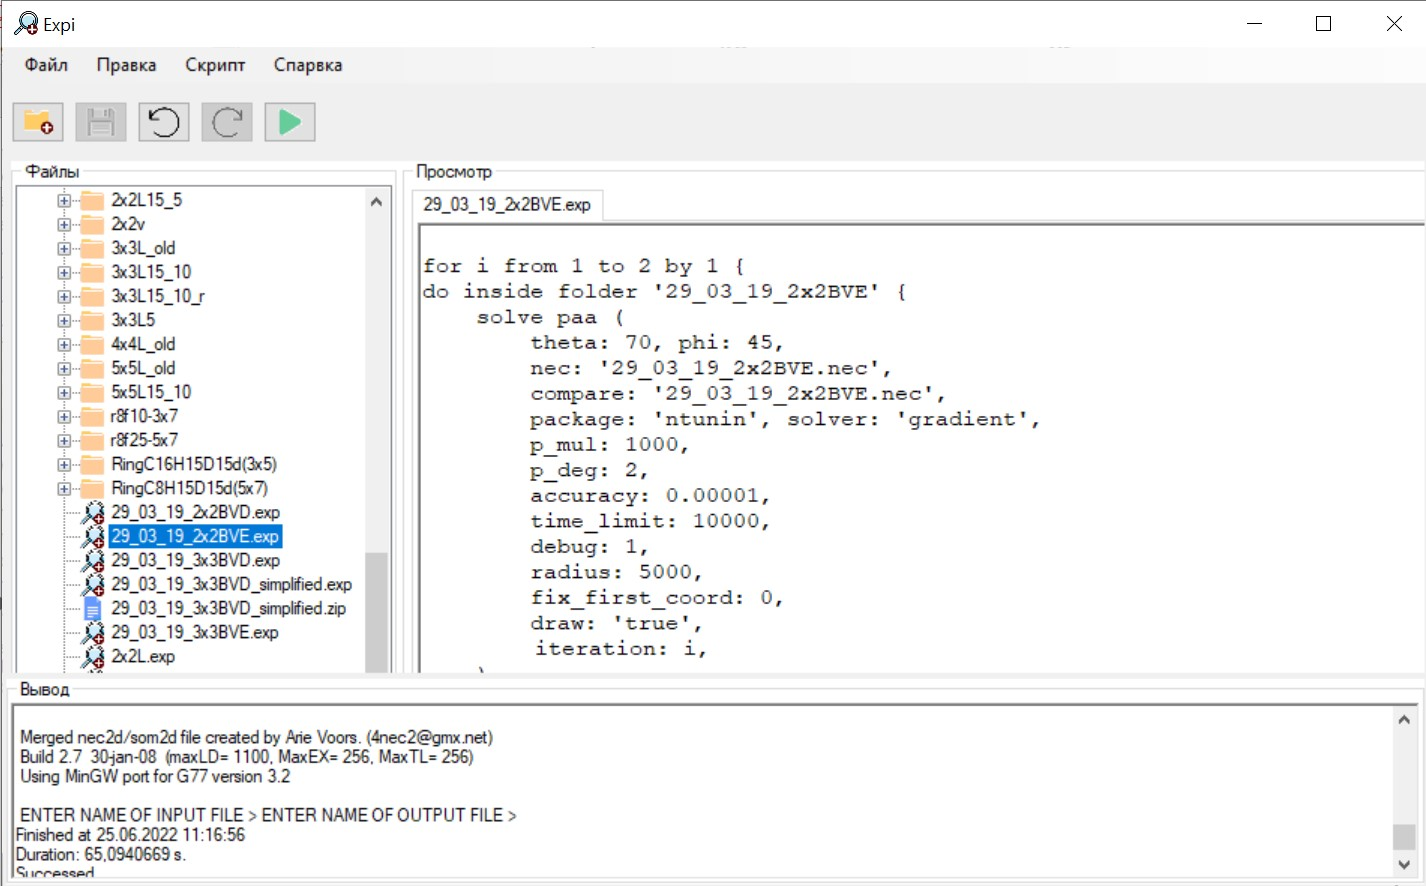
\includegraphics[width=\linewidth]{expi_script.jpeg}
  \caption{Редактор исполняемых файлов}
  \label{ic:applic_b_edit}
\end{figure}

\begin{figure}[h!]
  \centering
  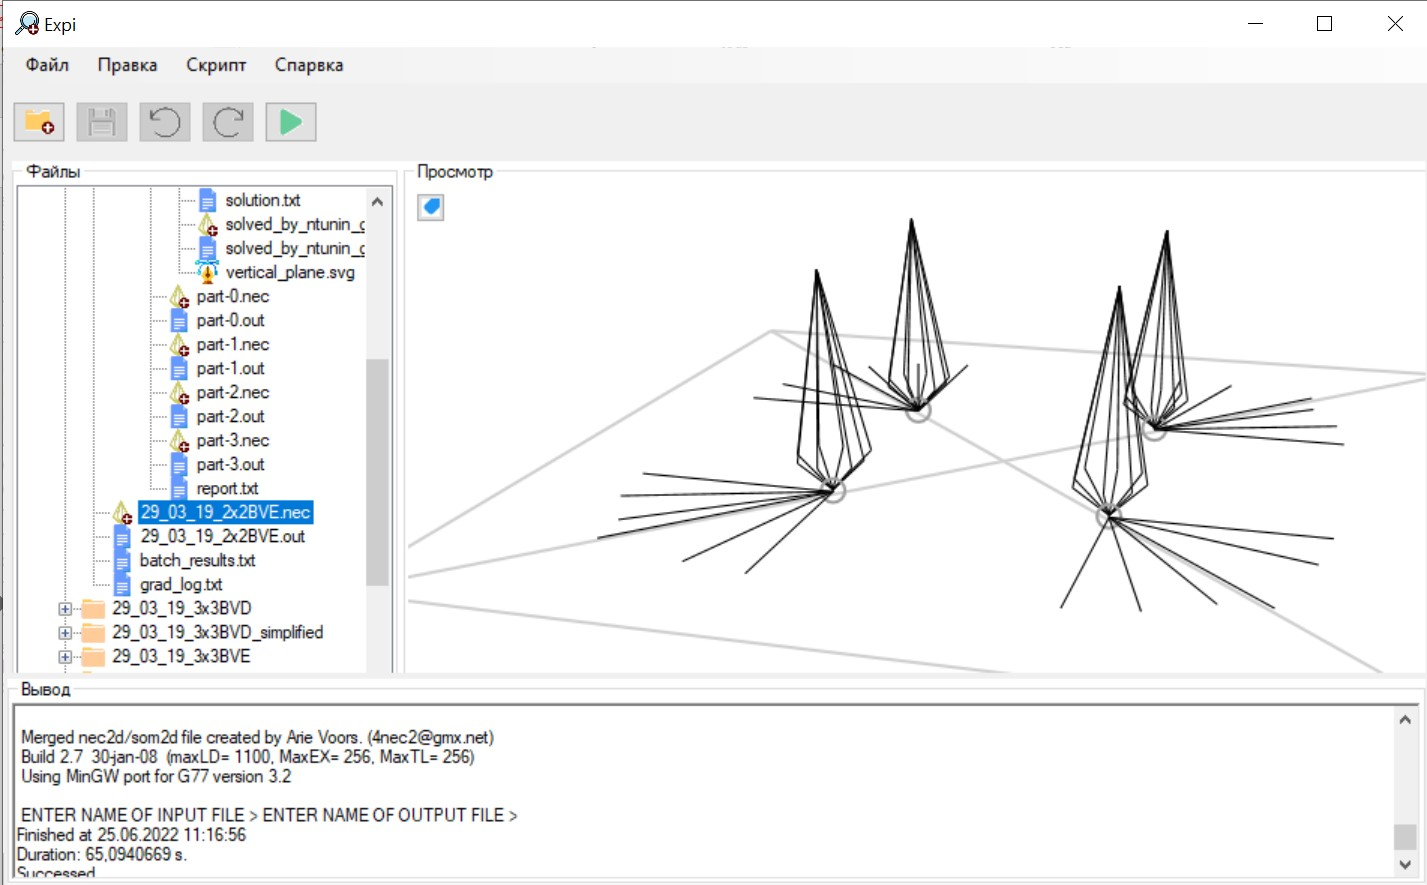
\includegraphics[width=\linewidth]{expi_paa.jpeg}
  \caption{Предпросмотр геометрии}
  \label{ic:applic_b_preview}
\end{figure}

\begin{figure}[h!]
  \centering
  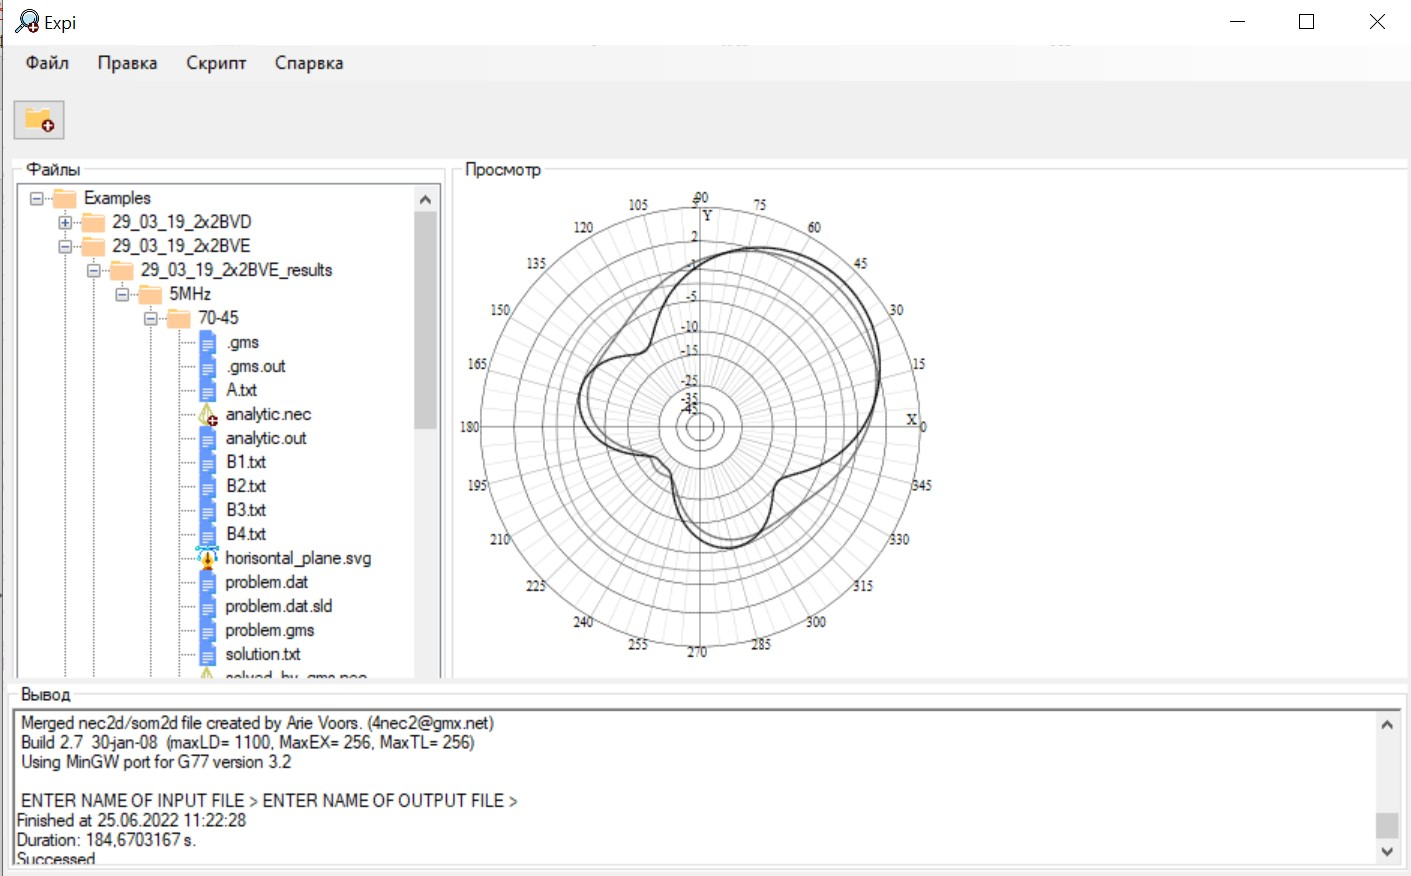
\includegraphics[width=\linewidth]{expi_results.jpeg}
  \caption{Предпросмотр результатов}
  \label{ic:applic_b_results}
\end{figure}

\subsection*{Языковые конструкции}
Комплекс <<Expi>> является, по сути, скриптовым интерпретатором одноименного языка, также разработанного автором в рамках текущей работы. Далее приводятся основные синтаксические конструкции.

\begin{lstlisting}[caption={Переменные}, label={experiment}]
def x = 1
def point = (0, 0, 1)
\end{lstlisting}

\begin{lstlisting}[caption={Сегментированный провод}, label={experiment}]
(0, 0, 0) -> (1, 0, 1) -> (0, 0, 5)
(0, 0, 0) -> (1, 0, 1) ~1v~ (0, 0, 5)
(0, 0, 0) -> (1, 0, 1) ~1+0.5iA~ (0, 0, 5)
\end{lstlisting}

\begin{lstlisting}[caption={Линейные преобразования}, label={experiment}]
translate x to 0.5
translate to (0, 0, 1)
rotate around z by pi/2
\end{lstlisting}

\begin{lstlisting}[caption={Циклы}, label={experiment}]

for angle from 0 to 2 * pi by pi/8 {
   rotate around z by angle
   (0, 0, 0) -> (1, 0, 0)
}

for angle from 0 up to 2 * pi by pi/8 {
   rotate around z by angle
   (0, 0, 0) -> (1, 0, 0)
}

\end{lstlisting}


\begin{lstlisting}[caption={Группы команд}, label={experiment}]
def Emitter {
    for angle from 0 to 2 * pi by pi/8 {
       rotate around z by angle
       (0, 0, 0) -> (1, 0, 0)
    }
}

translate x to -5
Emitter
translate x to 5
Emitter
\end{lstlisting}

\begin{lstlisting}[caption={Оптимизация направленности ФАР}, label={experiment}]
solve paa (
    n: 'bve_2x2.nec',
    theta: 70,
    phi: 45,
    p: 'ntunin',
    s: 'grad',
    c: 'bve.nec',
    p_mul: 1000000,
    p_deg: 4,
    time_limit: 1000,
    accuracy: 0.000001
)
\end{lstlisting}



\begin{lstlisting}[caption={Полный текст примера вычислительного эксперимента}, label={experiment}]

def knees = 8
def height = 15
def kneeWidth = 2.5
def base = 0.5
def rize = 2
def radialsCount = 6
def radialLength = 15
def size = 2
def distance = 20

def Drop {
   def step = 2 * pi / knees
   for angle from 0 to 2 * pi by step {
      rotate around z by angle
      (0, 0, 0) -> (kneeWidth, 0, kneeWidth) -> (0, 0, height)
   }
}

def BVE {
   (0, 0, 0) ~1v~ (0, 0, base)
   def step = pi / 2 / (radialsCount - 1)
   for i from 0 to  radialsCount  by 1 {
       rotate around z by i * step
       (0, 0, 0) -> (radialLength, 0, 0)
   }
   translate z to base
   Drop
}

def PlaceBVE {
   translate to (x, y, 0)
   rotate around z by angle
   BVE
}

def PAA {
   def width = (size - 1) * distance
   def left = -width/2
   def right = width/2
   def top = width/2
   def bottom = -width/2

   PlaceBVE(x: left, y: top, angle: pi / 2)
   PlaceBVE(x: right, y: top, angle: 0)
   PlaceBVE(x: right, y: bottom, angle: -pi / 2)
   PlaceBVE(x: left, y: bottom, angle: pi)
}

def ExportPAA {
    export nec (n: 'bve_${size}x${size}.nec', f: 5, g: 'real') {
        translate z to rize
        PAA
    }
}

def One {
    (0, 0, 0) ~1v~ (0, 0, base)
    def oneRadialsCount = (radialsCount - 1) * 4
    def step = 2 * pi / (oneRadialsCount - 1)
    for i from 0 to  oneRadialsCount by 1 {
        rotate around z by i * step
        (0, 0, 0) -> (radialLength, 0, 0)
    }
    translate z to base
    Drop
}

def ExportOne {
    export nec (n: 'bve.nec', f: 5, g: 'real') {
        translate z to rize
        One
    }
}

do inside folder '05.04.22' {
    ExportOne
    ExportPAA

    solve paa (
        n: 'bve_${size}x${size}.nec',
        theta: 70,
        phi: 45,
        p: 'ntunin',
        s: 'grad',
        c: 'bve.nec',
        p_mul: 1000000,
        p_deg: 4,
        time_limit: 1000,
        accuracy: 0.000001
    )
    solve paa (
        n: 'old_bve_${size}x${size}.nec',
        theta: 70,
        phi: 45,
        p: 'ntunin',
        s: 'grad',
        c: 'bve.nec',
        p_mul: 1000000,
        p_deg: 4,
        time_limit: 1000,
        accuracy: 0.000001
    )
}

\end{lstlisting}

\subsection*{Свидетельство о государственной регистрации}

\begin{figure}
\center{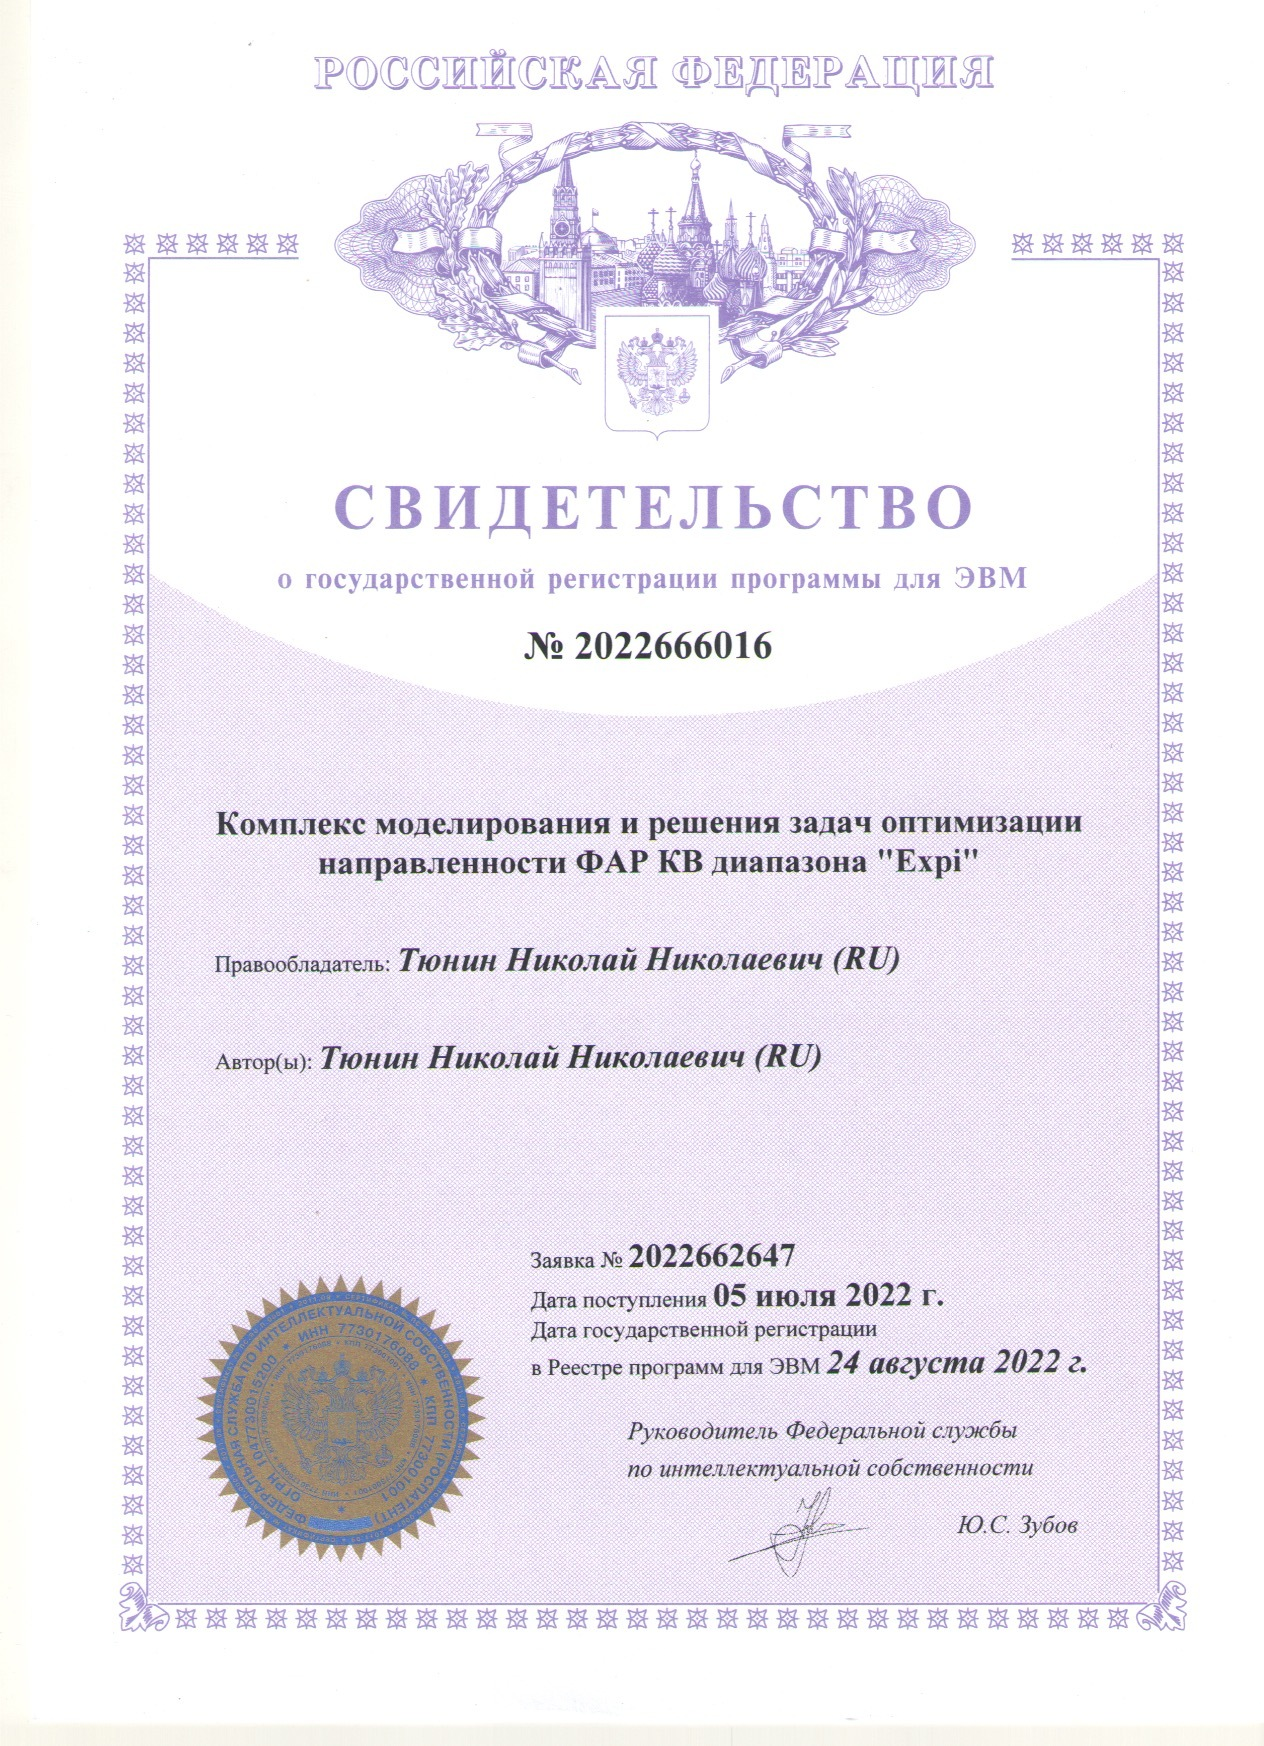
\includegraphics[width=0.95\linewidth]{expi_reg.jpeg}}
\caption{Свидетельство о государственной регистрации}
\label{ris:expi_reg}
\end{figure}       % Приложения
%\clearpage
\ifdefmacro{\microtypesetup}{\microtypesetup{protrusion=false}}{} % не рекомендуется применять пакет микротипографики к автоматически генерируемым спискам
\listoffigures  % Список изображений

%%% Список таблиц %%%
% (ГОСТ Р 7.0.11-2011, 5.3.10)
\clearpage
\listoftables   % Список таблиц
\ifdefmacro{\microtypesetup}{\microtypesetup{protrusion=true}}{}
\newpage           % Списки таблиц и изображений (иллюстративный материал)

\setcounter{totalchapter}{\value{chapter}} % Подсчёт количества глав

%%% Настройки для приложений
\appendix
% Оформление заголовков приложений ближе к ГОСТ:
\setlength{\midchapskip}{20pt}
\renewcommand*{\afterchapternum}{\par\nobreak\vskip \midchapskip}
\renewcommand\thechapter{\Asbuk{chapter}} % Чтобы приложения русскими буквами нумеровались

%\chapter*{ПРИЛОЖЕНИЯ}
\addcontentsline{toc}{chapter}{ПРИЛОЖЕНИЯ}
\section*{Приложение А}\label{sec:applic_a}
\addcontentsline{toc}{section}{Приложение A}
Здесь приводится подробное описание алгоритма исследования структуры локальных оптимумов. Для удобства изложения, алгоритм разбит
на процедуры: <<Одномерный поиск>>, <<Градиентный подъем>> и <<Исследование локальных оптимумов>>.
\\ \\
\noindent{\textbf{ 1. Одномерный поиск.}}

\noindent{\textbf{ Дано:}}
\begin{itemize}
  \item вектор начального решения $\textbf{x}$ размерности $2N$,
  \item вектор направления одномерного поиска $\textbf{d}$ размерности $2N$,
  \item точность вычислений $\epsilon_{1dim}$.
\end{itemize}
\noindent{\textbf{ Требуется:}} найти вектор $\textbf{x}' = \textbf{x} + \gamma \textbf{d}$ такой, что
\begin{itemize}
  \item $\tilde{F}(\textbf{x}) < \tilde{F}(\textbf{x}'),$
  \item $\tilde{F}(\textbf{x} + (\gamma + \epsilon_{1dim}) \textbf{d}) < \tilde{F}(\textbf{x}').$
\end{itemize}
\begin{enumerate}
  \item Инициализировать параметр одномерного поиска $\beta := 1$, вектор $\textbf{x}' := \textbf{x}$, счетчик итераций $j := 1$.
  \item Если $\tilde{F}(\textbf{x}' + \beta \textbf{d}) < \tilde{F}(\textbf{x}')$, то уменьшить $\beta := \beta / 2$.
  В противном случае, в зависимости от значения счетчика:\\
  при $j = 1$ положить $\textbf{x}_a := \textbf{x}'$,\\
  при $j = 2$ положить $\textbf{x}_b := \textbf{x}'$,\\
  при $j = 3$ положить $\textbf{x}_c := \textbf{x}'$,\\
  при $j > 3$ положить $\textbf{x}_a := \textbf{x}_b$, $\textbf{x}_b := \textbf{x}_c$, $\textbf{x}_c := \textbf{x}'$.\\
  При этом, вне зависимости от значений счетчика, $\beta := 2\beta$,\\
  $\textbf{x}' := \textbf{x}' + \beta \textbf{d}.$
  \item Если $\beta < \epsilon_{1dim}$ и $j < 3$, вернуть $\textbf{x}'$.
  \item Если $\beta < \epsilon_{1dim}$ и $j \geq 3$, то переходим к шагу 5, иначе - на шаг 2.
  \item По точкам $\textbf{x}_a, \textbf{x}_b, \textbf{x}_c$ строим квадратичную аппроксимацию:
   $$\textbf{x}^{*} := (\textbf{x}_b - 3 \beta \textbf{d}) +
   \left(\beta\left(1 + \frac{\tilde{F}(\textbf{x}_a) - \tilde{F}(\textbf{x}_c)}{2(\tilde{F}(\textbf{x}_a) -
   2\tilde{F}(\textbf{x}_b) + \tilde{F}(\textbf{x}_c))}\right)\right)\textbf{d}.$$\\
\end{enumerate}
{ \textbf{2. Градиентный подъем.}}
\\ \\
\noindent{\textbf{Дано:}}
\begin{itemize}
  \item вектор начального решения $\textbf{x}_0$ размерности $2N$,
  \item точность вычислений $\epsilon_{grad}$,
  \item точность вычислений одномерного поиска $\epsilon_{1dim}$,
  \item время принудительного завершения работы алгоритма $time_{finish}.$\\
\end{itemize}
\noindent{\textbf{Требуется:}} найти вектор $\textbf{x}$ такой, что
для всех $$\textbf{d}, |\textbf{d}| = 1 \text{~выполняется~} \tilde{F}(\textbf{x} + (\epsilon_{grad})\textbf{d}) < \tilde{F}(\textbf{x})$$.\\
\begin{enumerate}
  \item $\textbf{x} := \textbf{x}_0.$
  \item Вычислить и нормировать градиент целевой функции:
   $$\textbf{d} := \frac{\nabla \tilde{F}(\textbf{x})}{|\nabla \tilde{F}(\textbf{x})|}.$$
  \item Вычислить $\textbf{x}^{*}$ алгоритмом одномерного поиска~1 с параметрами $\textbf{x}, \textbf{d}, \epsilon_{1dim}.$
  \item Записать в $time$ текущее время. Если $time \geq time_{finish}$, вернуть $\textbf{x}^{*}$.
  \item Если $|\tilde{F}(\textbf{x}) - \tilde{F}(\textbf{x}^{*})| < \epsilon_{grad}$, вернуть $\textbf{x}^{*}$, иначе положить $\textbf{x} = \textbf{x}^{*}$ и повторить~шаги~2-5.\\ \\
\end{enumerate}

\noindent{\textbf{ 3. Исследование локальных оптимумов.}}
\\ \\
\noindent{\textbf{Дано:}}
\begin{itemize}
  \item $x_{\max}$ как верхняя оценка нормы допустимой области,
  \item точность вычислений $\epsilon_{grad}$,
  \item точность вычислений одномерного поиска $\epsilon_{1dim}$,
  \item время принудительного завершения работы алгоритма $time_{finish}$,
  \item максимально допустимая норма вектора ${\textbf{y}}$, обозначаемая за ${\textbf{y}}_{\max}$.\\
\end{itemize}

\noindent{\textbf{Требуется:}} провести исследование структуры локальных оптимумов, как описано в разделе~\ref{sec:exp}.\\

\begin{enumerate}
  \item Инициализировать каждую компоненту начального вектора $x_{0,i = \overline{1,2N}}$ равномерно распределенной в интервале $[-x_{\max}, x_{\max}]$
  величиной.
  \item Вычисляем допустимый вектор $\textbf{x}$ путем масштабирования $\textbf{x}_0$ в допустимую область:
  $$\textbf{x} := (\max_{k=\overline{1,n}} {\textbf{x}_0}^T \textbf{H}^{(k)}{\textbf{x}_0})^{-1/2} {\textbf{x}_0}.$$
  \item Вычислить ${\textbf{x}^{*}}$ алгоритмом градиентного подъема~(2) с параметрами ${\textbf{x}}, \epsilon_{grad}, \epsilon_{1dim}, time_{finish}.$
  \item Записать в $time$ текущее время. Если $time$ < $time_{finish}$, перейти на шаг~1.
  \item Для каждого найденного решения установить ${\textbf{x}_0^{*}} = {\textbf{x}^{*}}$, составить линеаризованную задачу~(\ref{eq:task5}) и найти
  ее решение ${\textbf{x}_{lp}^{*}}$.
  \item Исключить решения, для которых $|{\textbf{x}_0^{*}} - {\textbf{x}_{lp}^{*}}| > {\textbf{y}_{\max}}$. В случае оставшихся решений установить
  $\textbf{x} = {\textbf{x}_{lp}^{*}}$ и повторить шаги~2-3. Оценить норму разницы $|{\textbf{x}_0^{*}} - {\textbf{x}^{*}}|$. Вернуть ${\textbf{x}_0^{*}}$ с
  лучшим значением $\tilde{F}({\textbf{x}_0^{*}})$ в качестве результата.
\end{enumerate}

\section*{Приложение Б}
\addcontentsline{toc}{section}{Приложение Б}
\label{sec:applic_b}
Комплекс моделирования и решения задач оптимизации направленности ФАР КВ диапазона <<Expi>> предназначен для моделирования антенных систем и вычисления управляющих параметров фазированных антенных решеток (ФАР).Регистрируемая программа для ЭВМ применима в радиотехнике
при оптимизации направленного излучения ФАР КВ диапазона.Программа позволяет запускать файлы заданного формата с инструкциями по организации вычислительного эксперимента, редактировать их, визуализировать результаты.
Здесь приводится графический интерфейс и функциональные возможности разработанного в рамках текущей работы программного комплекса <<Expi>>.

\subsection*{Графический интерфейс}
  Программное окно разделено на три части: обозреватель текущей директории, окно вывода и рабочая область. Содержимое рабочей области меняется, в зависимости от выбранного файла. В случае, если выбран файл эксперимента~(.exp), оно представляет собой редактор текстового файла~(рис.~(\ref{ic:applic_b_edit})). Для файла формата .nec будет представлен обозреватель геометрии антенной системы~(рис.~(\ref{ic:applic_b_preview})), Для файлов формата .svg, в которые производится запись диаграмм направленности, приводится предпросмотр данного графического формата~(рис.~(\ref{ic:applic_b_results})).

\begin{figure}[h!]
  \centering
  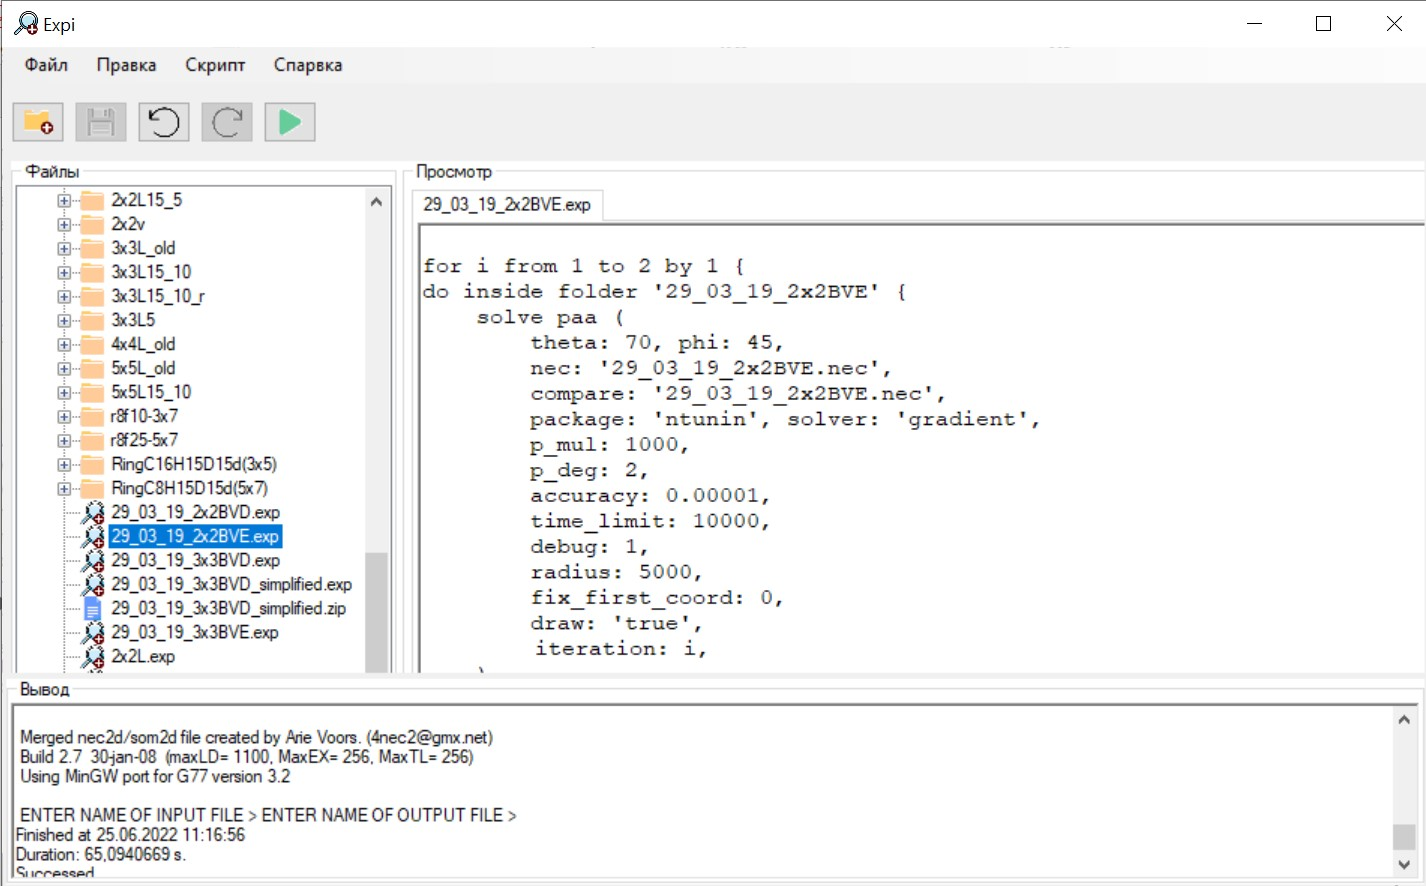
\includegraphics[width=\linewidth]{expi_script.jpeg}
  \caption{Редактор исполняемых файлов}
  \label{ic:applic_b_edit}
\end{figure}

\begin{figure}[h!]
  \centering
  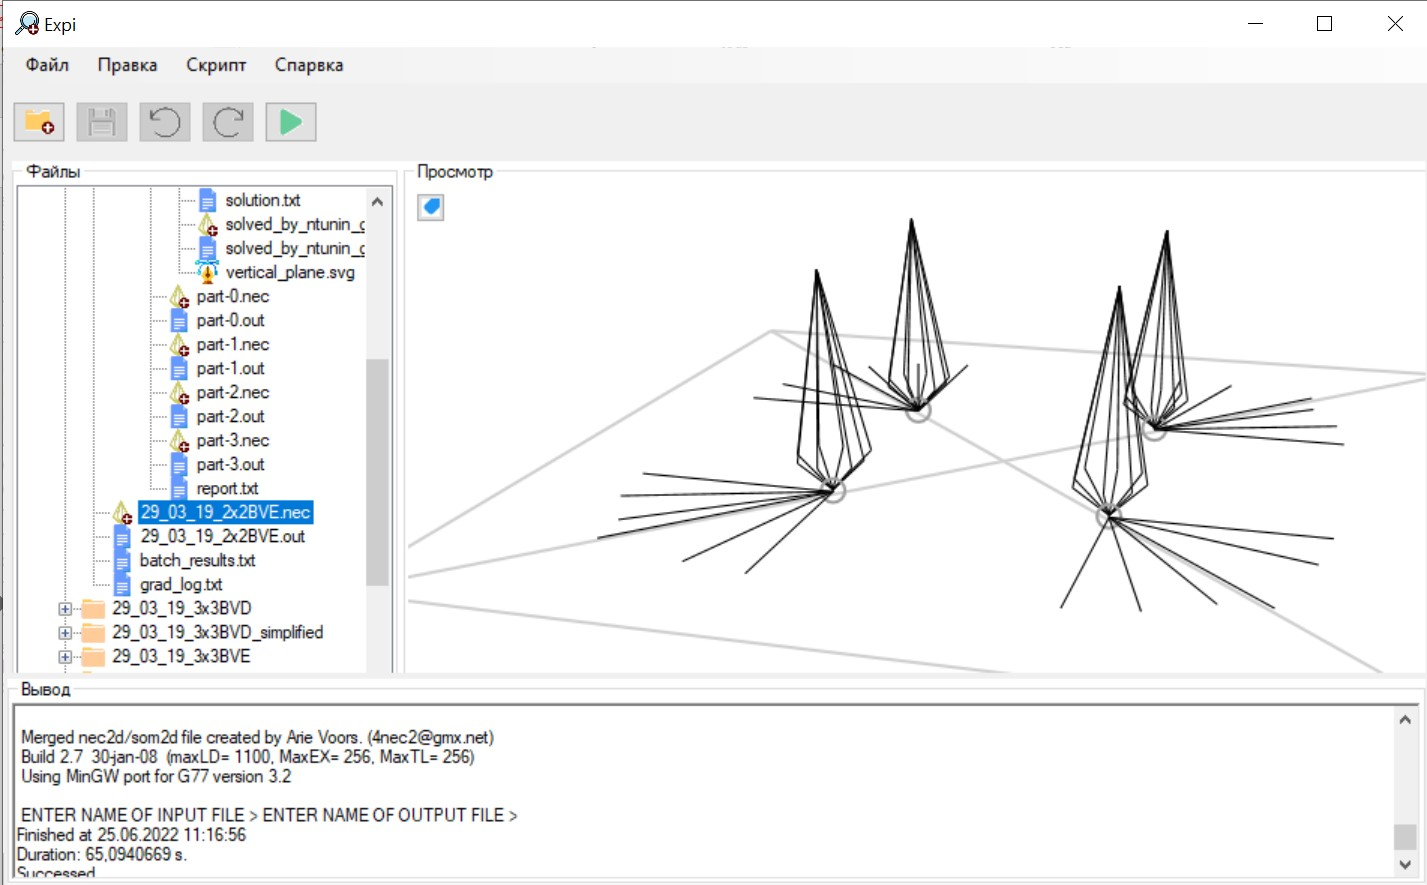
\includegraphics[width=\linewidth]{expi_paa.jpeg}
  \caption{Предпросмотр геометрии}
  \label{ic:applic_b_preview}
\end{figure}

\begin{figure}[h!]
  \centering
  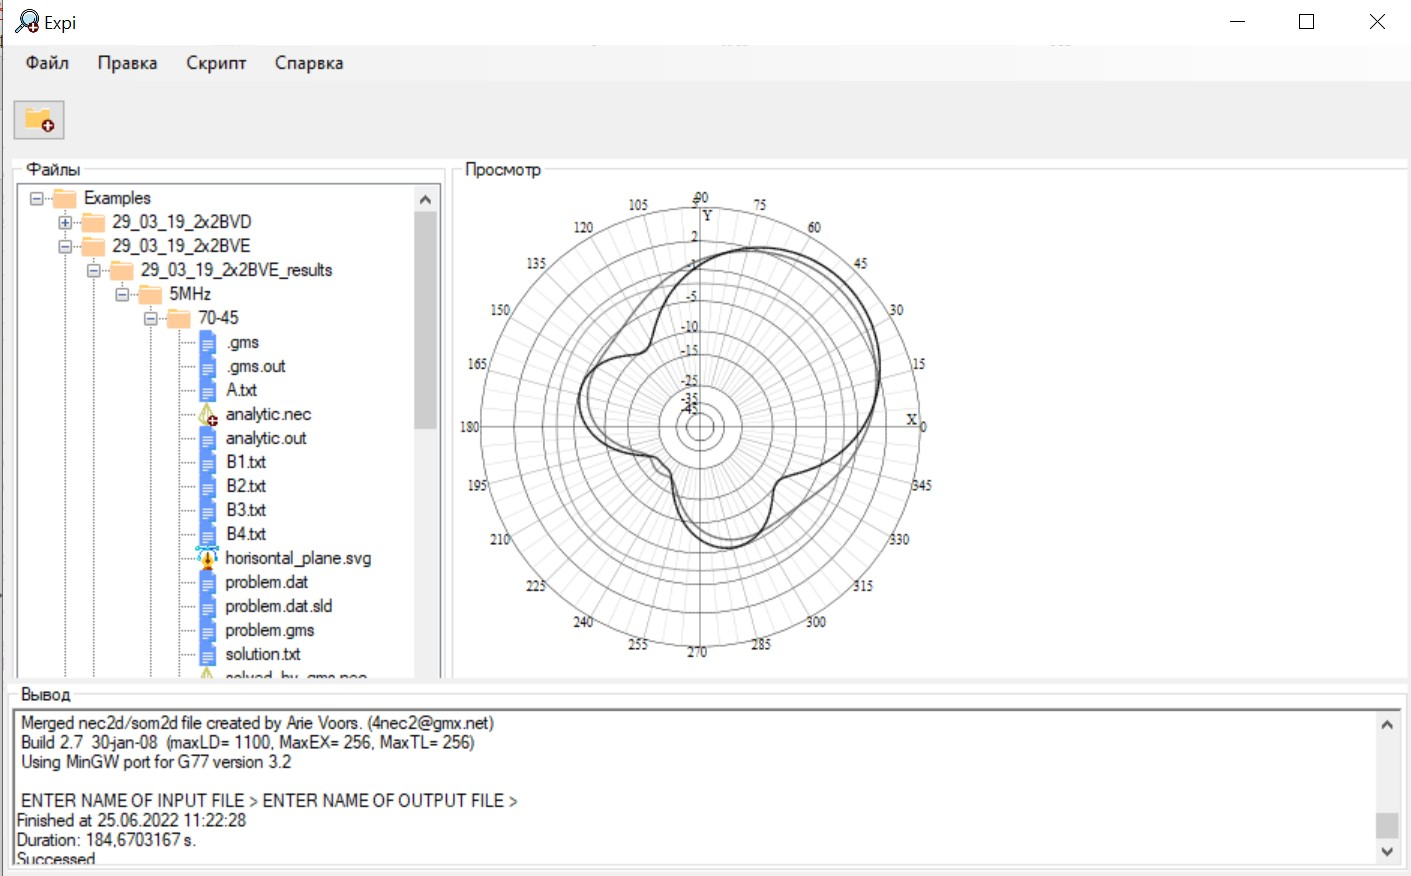
\includegraphics[width=\linewidth]{expi_results.jpeg}
  \caption{Предпросмотр результатов}
  \label{ic:applic_b_results}
\end{figure}

\subsection*{Языковые конструкции}
Комплекс <<Expi>> является, по сути, скриптовым интерпретатором одноименного языка, также разработанного автором в рамках текущей работы. Далее приводятся основные синтаксические конструкции.

\begin{lstlisting}[caption={Переменные}, label={experiment}]
def x = 1
def point = (0, 0, 1)
\end{lstlisting}

\begin{lstlisting}[caption={Сегментированный провод}, label={experiment}]
(0, 0, 0) -> (1, 0, 1) -> (0, 0, 5)
(0, 0, 0) -> (1, 0, 1) ~1v~ (0, 0, 5)
(0, 0, 0) -> (1, 0, 1) ~1+0.5iA~ (0, 0, 5)
\end{lstlisting}

\begin{lstlisting}[caption={Линейные преобразования}, label={experiment}]
translate x to 0.5
translate to (0, 0, 1)
rotate around z by pi/2
\end{lstlisting}

\begin{lstlisting}[caption={Циклы}, label={experiment}]

for angle from 0 to 2 * pi by pi/8 {
   rotate around z by angle
   (0, 0, 0) -> (1, 0, 0)
}

for angle from 0 up to 2 * pi by pi/8 {
   rotate around z by angle
   (0, 0, 0) -> (1, 0, 0)
}

\end{lstlisting}


\begin{lstlisting}[caption={Группы команд}, label={experiment}]
def Emitter {
    for angle from 0 to 2 * pi by pi/8 {
       rotate around z by angle
       (0, 0, 0) -> (1, 0, 0)
    }
}

translate x to -5
Emitter
translate x to 5
Emitter
\end{lstlisting}

\begin{lstlisting}[caption={Оптимизация направленности ФАР}, label={experiment}]
solve paa (
    n: 'bve_2x2.nec',
    theta: 70,
    phi: 45,
    p: 'ntunin',
    s: 'grad',
    c: 'bve.nec',
    p_mul: 1000000,
    p_deg: 4,
    time_limit: 1000,
    accuracy: 0.000001
)
\end{lstlisting}



\begin{lstlisting}[caption={Полный текст примера вычислительного эксперимента}, label={experiment}]

def knees = 8
def height = 15
def kneeWidth = 2.5
def base = 0.5
def rize = 2
def radialsCount = 6
def radialLength = 15
def size = 2
def distance = 20

def Drop {
   def step = 2 * pi / knees
   for angle from 0 to 2 * pi by step {
      rotate around z by angle
      (0, 0, 0) -> (kneeWidth, 0, kneeWidth) -> (0, 0, height)
   }
}

def BVE {
   (0, 0, 0) ~1v~ (0, 0, base)
   def step = pi / 2 / (radialsCount - 1)
   for i from 0 to  radialsCount  by 1 {
       rotate around z by i * step
       (0, 0, 0) -> (radialLength, 0, 0)
   }
   translate z to base
   Drop
}

def PlaceBVE {
   translate to (x, y, 0)
   rotate around z by angle
   BVE
}

def PAA {
   def width = (size - 1) * distance
   def left = -width/2
   def right = width/2
   def top = width/2
   def bottom = -width/2

   PlaceBVE(x: left, y: top, angle: pi / 2)
   PlaceBVE(x: right, y: top, angle: 0)
   PlaceBVE(x: right, y: bottom, angle: -pi / 2)
   PlaceBVE(x: left, y: bottom, angle: pi)
}

def ExportPAA {
    export nec (n: 'bve_${size}x${size}.nec', f: 5, g: 'real') {
        translate z to rize
        PAA
    }
}

def One {
    (0, 0, 0) ~1v~ (0, 0, base)
    def oneRadialsCount = (radialsCount - 1) * 4
    def step = 2 * pi / (oneRadialsCount - 1)
    for i from 0 to  oneRadialsCount by 1 {
        rotate around z by i * step
        (0, 0, 0) -> (radialLength, 0, 0)
    }
    translate z to base
    Drop
}

def ExportOne {
    export nec (n: 'bve.nec', f: 5, g: 'real') {
        translate z to rize
        One
    }
}

do inside folder '05.04.22' {
    ExportOne
    ExportPAA

    solve paa (
        n: 'bve_${size}x${size}.nec',
        theta: 70,
        phi: 45,
        p: 'ntunin',
        s: 'grad',
        c: 'bve.nec',
        p_mul: 1000000,
        p_deg: 4,
        time_limit: 1000,
        accuracy: 0.000001
    )
    solve paa (
        n: 'old_bve_${size}x${size}.nec',
        theta: 70,
        phi: 45,
        p: 'ntunin',
        s: 'grad',
        c: 'bve.nec',
        p_mul: 1000000,
        p_deg: 4,
        time_limit: 1000,
        accuracy: 0.000001
    )
}

\end{lstlisting}

\subsection*{Свидетельство о государственной регистрации}

\begin{figure}
\center{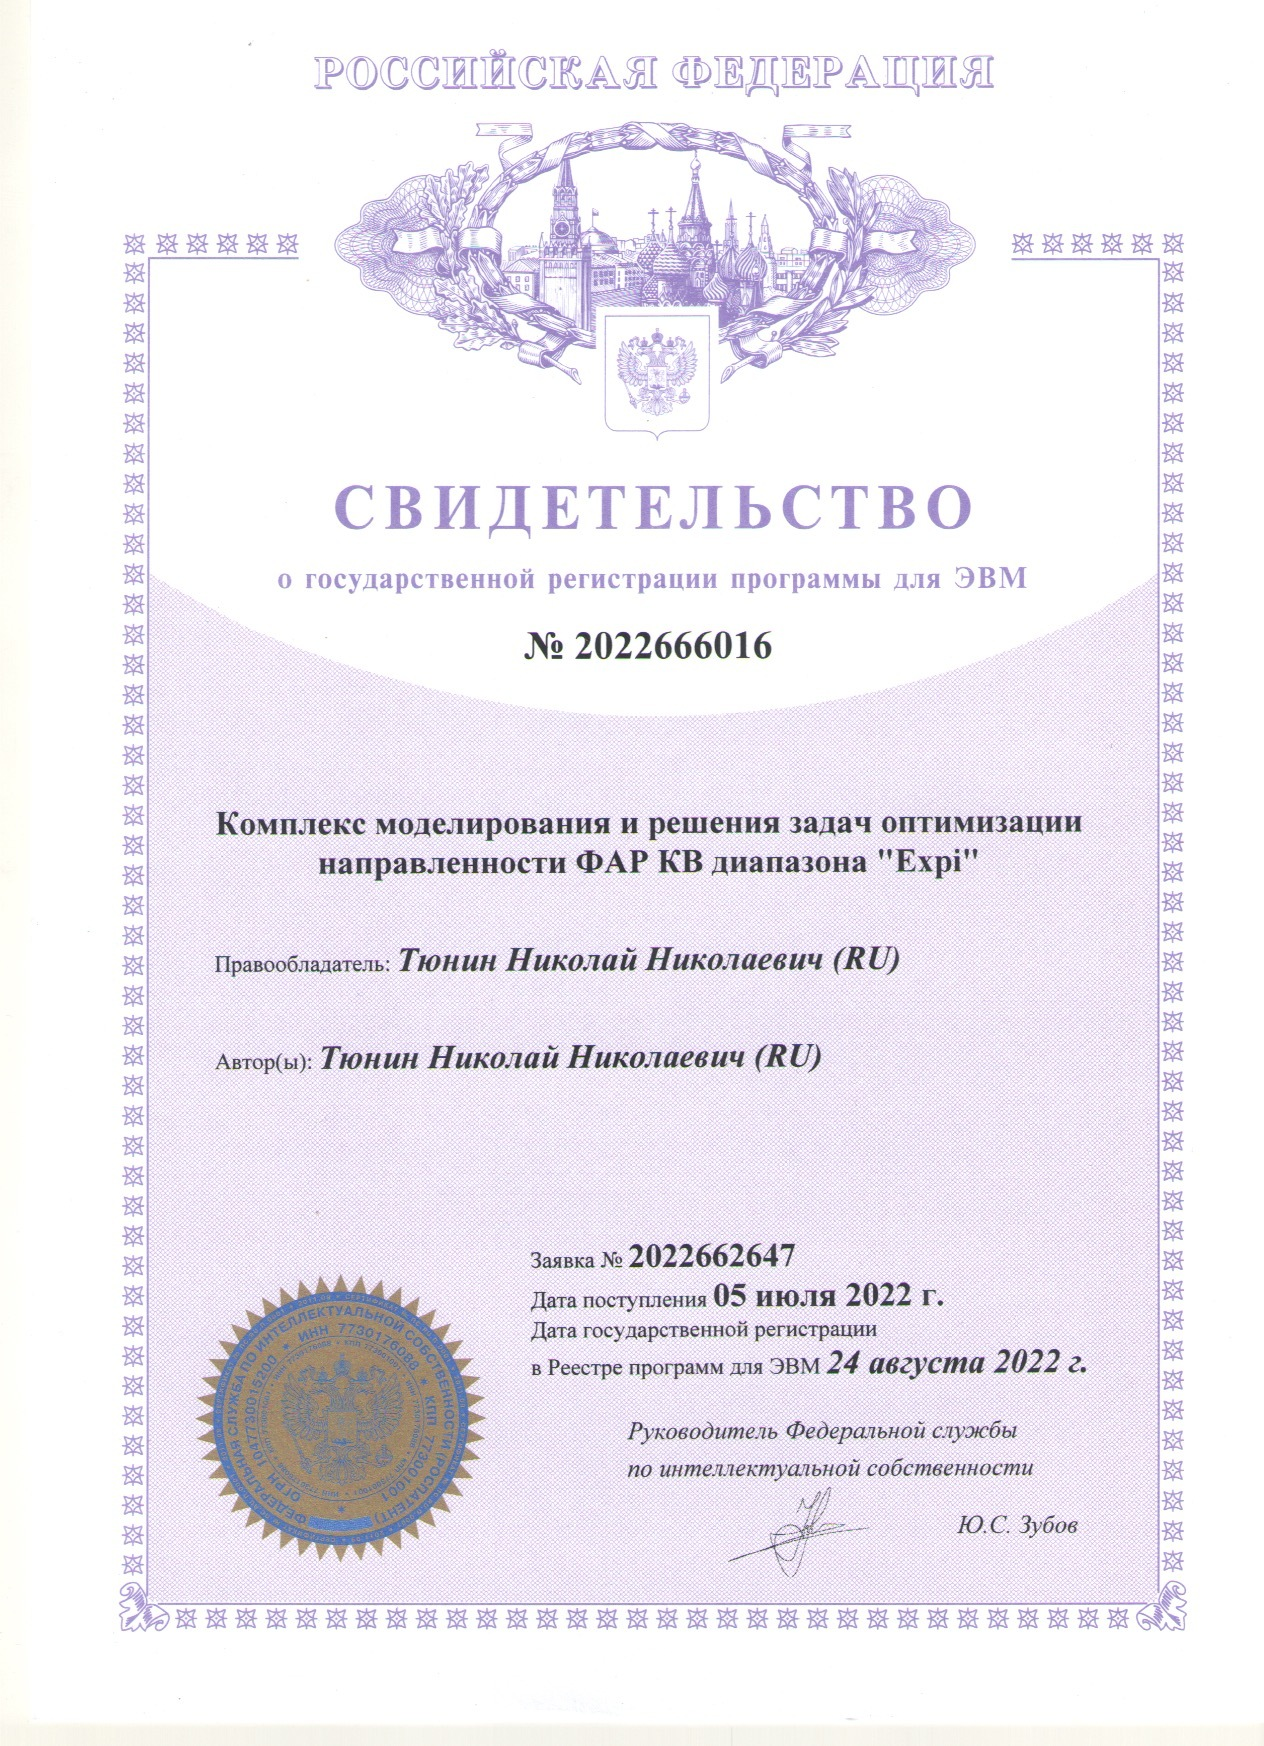
\includegraphics[width=0.95\linewidth]{expi_reg.jpeg}}
\caption{Свидетельство о государственной регистрации}
\label{ris:expi_reg}
\end{figure}         % Приложения

\setcounter{totalappendix}{\value{chapter}} % Подсчёт количества приложений

\end{document}
